% Options for packages loaded elsewhere
\PassOptionsToPackage{unicode}{hyperref}
\PassOptionsToPackage{hyphens}{url}
%
\documentclass[
]{book}
\usepackage{amsmath,amssymb}
\usepackage{lmodern}
\usepackage{iftex}
\ifPDFTeX
  \usepackage[T1]{fontenc}
  \usepackage[utf8]{inputenc}
  \usepackage{textcomp} % provide euro and other symbols
\else % if luatex or xetex
  \usepackage{unicode-math}
  \defaultfontfeatures{Scale=MatchLowercase}
  \defaultfontfeatures[\rmfamily]{Ligatures=TeX,Scale=1}
\fi
% Use upquote if available, for straight quotes in verbatim environments
\IfFileExists{upquote.sty}{\usepackage{upquote}}{}
\IfFileExists{microtype.sty}{% use microtype if available
  \usepackage[]{microtype}
  \UseMicrotypeSet[protrusion]{basicmath} % disable protrusion for tt fonts
}{}
\makeatletter
\@ifundefined{KOMAClassName}{% if non-KOMA class
  \IfFileExists{parskip.sty}{%
    \usepackage{parskip}
  }{% else
    \setlength{\parindent}{0pt}
    \setlength{\parskip}{6pt plus 2pt minus 1pt}}
}{% if KOMA class
  \KOMAoptions{parskip=half}}
\makeatother
\usepackage{xcolor}
\usepackage{color}
\usepackage{fancyvrb}
\newcommand{\VerbBar}{|}
\newcommand{\VERB}{\Verb[commandchars=\\\{\}]}
\DefineVerbatimEnvironment{Highlighting}{Verbatim}{commandchars=\\\{\}}
% Add ',fontsize=\small' for more characters per line
\usepackage{framed}
\definecolor{shadecolor}{RGB}{248,248,248}
\newenvironment{Shaded}{\begin{snugshade}}{\end{snugshade}}
\newcommand{\AlertTok}[1]{\textcolor[rgb]{0.94,0.16,0.16}{#1}}
\newcommand{\AnnotationTok}[1]{\textcolor[rgb]{0.56,0.35,0.01}{\textbf{\textit{#1}}}}
\newcommand{\AttributeTok}[1]{\textcolor[rgb]{0.77,0.63,0.00}{#1}}
\newcommand{\BaseNTok}[1]{\textcolor[rgb]{0.00,0.00,0.81}{#1}}
\newcommand{\BuiltInTok}[1]{#1}
\newcommand{\CharTok}[1]{\textcolor[rgb]{0.31,0.60,0.02}{#1}}
\newcommand{\CommentTok}[1]{\textcolor[rgb]{0.56,0.35,0.01}{\textit{#1}}}
\newcommand{\CommentVarTok}[1]{\textcolor[rgb]{0.56,0.35,0.01}{\textbf{\textit{#1}}}}
\newcommand{\ConstantTok}[1]{\textcolor[rgb]{0.00,0.00,0.00}{#1}}
\newcommand{\ControlFlowTok}[1]{\textcolor[rgb]{0.13,0.29,0.53}{\textbf{#1}}}
\newcommand{\DataTypeTok}[1]{\textcolor[rgb]{0.13,0.29,0.53}{#1}}
\newcommand{\DecValTok}[1]{\textcolor[rgb]{0.00,0.00,0.81}{#1}}
\newcommand{\DocumentationTok}[1]{\textcolor[rgb]{0.56,0.35,0.01}{\textbf{\textit{#1}}}}
\newcommand{\ErrorTok}[1]{\textcolor[rgb]{0.64,0.00,0.00}{\textbf{#1}}}
\newcommand{\ExtensionTok}[1]{#1}
\newcommand{\FloatTok}[1]{\textcolor[rgb]{0.00,0.00,0.81}{#1}}
\newcommand{\FunctionTok}[1]{\textcolor[rgb]{0.00,0.00,0.00}{#1}}
\newcommand{\ImportTok}[1]{#1}
\newcommand{\InformationTok}[1]{\textcolor[rgb]{0.56,0.35,0.01}{\textbf{\textit{#1}}}}
\newcommand{\KeywordTok}[1]{\textcolor[rgb]{0.13,0.29,0.53}{\textbf{#1}}}
\newcommand{\NormalTok}[1]{#1}
\newcommand{\OperatorTok}[1]{\textcolor[rgb]{0.81,0.36,0.00}{\textbf{#1}}}
\newcommand{\OtherTok}[1]{\textcolor[rgb]{0.56,0.35,0.01}{#1}}
\newcommand{\PreprocessorTok}[1]{\textcolor[rgb]{0.56,0.35,0.01}{\textit{#1}}}
\newcommand{\RegionMarkerTok}[1]{#1}
\newcommand{\SpecialCharTok}[1]{\textcolor[rgb]{0.00,0.00,0.00}{#1}}
\newcommand{\SpecialStringTok}[1]{\textcolor[rgb]{0.31,0.60,0.02}{#1}}
\newcommand{\StringTok}[1]{\textcolor[rgb]{0.31,0.60,0.02}{#1}}
\newcommand{\VariableTok}[1]{\textcolor[rgb]{0.00,0.00,0.00}{#1}}
\newcommand{\VerbatimStringTok}[1]{\textcolor[rgb]{0.31,0.60,0.02}{#1}}
\newcommand{\WarningTok}[1]{\textcolor[rgb]{0.56,0.35,0.01}{\textbf{\textit{#1}}}}
\usepackage{longtable,booktabs,array}
\usepackage{calc} % for calculating minipage widths
% Correct order of tables after \paragraph or \subparagraph
\usepackage{etoolbox}
\makeatletter
\patchcmd\longtable{\par}{\if@noskipsec\mbox{}\fi\par}{}{}
\makeatother
% Allow footnotes in longtable head/foot
\IfFileExists{footnotehyper.sty}{\usepackage{footnotehyper}}{\usepackage{footnote}}
\makesavenoteenv{longtable}
\usepackage{graphicx}
\makeatletter
\def\maxwidth{\ifdim\Gin@nat@width>\linewidth\linewidth\else\Gin@nat@width\fi}
\def\maxheight{\ifdim\Gin@nat@height>\textheight\textheight\else\Gin@nat@height\fi}
\makeatother
% Scale images if necessary, so that they will not overflow the page
% margins by default, and it is still possible to overwrite the defaults
% using explicit options in \includegraphics[width, height, ...]{}
\setkeys{Gin}{width=\maxwidth,height=\maxheight,keepaspectratio}
% Set default figure placement to htbp
\makeatletter
\def\fps@figure{htbp}
\makeatother
\setlength{\emergencystretch}{3em} % prevent overfull lines
\providecommand{\tightlist}{%
  \setlength{\itemsep}{0pt}\setlength{\parskip}{0pt}}
\setcounter{secnumdepth}{5}
\usepackage{booktabs}
\usepackage{amsthm}
\usepackage[utf8]{inputenc}

\makeatletter
\def\thm@space@setup{%
  \thm@preskip=8pt plus 2pt minus 4pt
  \thm@postskip=\thm@preskip
}
\makeatother

\usepackage[spanish]{babel} % nuestro  
\graphicspath{{_bookdown_files/}}

\addto\captionsspanish{%
\renewcommand\chaptername{Lección}}
\addto\captionsspanish{%
\renewcommand\tablename{Tabla}}

\renewcommand\chaptername{Lección}
\renewcommand{\leq}{\leqslant}
\renewcommand{\geq}{\geqslant}
\usepackage{booktabs}
\usepackage{longtable}
\usepackage{array}
\usepackage{multirow}
\usepackage{wrapfig}
\usepackage{float}
\usepackage{colortbl}
\usepackage{pdflscape}
\usepackage{tabu}
\usepackage{threeparttable}
\usepackage{threeparttablex}
\usepackage[normalem]{ulem}
\usepackage{makecell}
\usepackage{xcolor}
\ifLuaTeX
  \usepackage{selnolig}  % disable illegal ligatures
\fi
\usepackage[]{natbib}
\bibliographystyle{apalike}
\IfFileExists{bookmark.sty}{\usepackage{bookmark}}{\usepackage{hyperref}}
\IfFileExists{xurl.sty}{\usepackage{xurl}}{} % add URL line breaks if available
\urlstyle{same} % disable monospaced font for URLs
\hypersetup{
  pdftitle={Bioestadística (Medicina UIB)},
  pdfauthor={Irene García, Francesc Rosselló},
  hidelinks,
  pdfcreator={LaTeX via pandoc}}

\title{Bioestadística (Medicina UIB)}
\author{Irene García, Francesc Rosselló}
\date{2023-06-05}

\usepackage{amsthm}
\newtheorem{theorem}{Teorema}[chapter]
\newtheorem{lemma}{Lema}[chapter]
\newtheorem{corollary}{Corolario}[chapter]
\newtheorem{proposition}{Proposition}[chapter]
\newtheorem{conjecture}{Conjecture}[chapter]
\theoremstyle{definition}
\newtheorem{definition}{Definición}[chapter]
\theoremstyle{definition}
\newtheorem{example}{Ejemplo}[chapter]
\theoremstyle{definition}
\newtheorem{exercise}{Ejercicio}[chapter]
\theoremstyle{definition}
\newtheorem{hypothesis}{Hypothesis}[chapter]
\theoremstyle{remark}
\newtheorem*{remark}{Nota}
\newtheorem*{solution}{Solución}
\begin{document}
\maketitle

{
\setcounter{tocdepth}{1}
\tableofcontents
}
\hypertarget{presentaciuxf3n}{%
\chapter*{Presentación}\label{presentaciuxf3n}}
\addcontentsline{toc}{chapter}{Presentación}

Esto es una edición en línea de los apuntes de \emph{Introducción a la Investigación en Salud y Bioestadística} del grado de Medicina de la UIB. El libro está escrito en \emph{R Markdown}, usando \emph{RStudio} como editor de textos y el paquete \textbf{bookdown} para convertir los ficheros \emph{markdown} en un libro. Este trabajo se publica bajo licencia \href{https://creativecommons.org/licenses/by-nc-nd/4.0/}{Atribución-No Comercial-SinDerivados 4.0}.

\textbf{Significado de algunas cajas}:

\begin{rmdimportant}
Material muy importante.
\end{rmdimportant}

\begin{rmdcaution}
¡Cuidado!
\end{rmdcaution}

\begin{rmdexercici}
Ejercicio.
\end{rmdexercici}

\begin{rmdcorbes}
Detalles matemáticos que os pueden interesar, pero que podéis obviar sin ningún problema.
\end{rmdcorbes}

\begin{rmdnote}
Comentario que queremos enfatizar.
\end{rmdnote}

\begin{rmdrecordau}
Comentario que queremos que recordéis
\end{rmdrecordau}

\begin{rmdromans}
Cuestión en la que queremos que caigáis en la cuenta.
\end{rmdromans}

\begin{rmderrorpetit}
Acabamos de matar un gatito
\end{rmderrorpetit}

\hypertarget{part-tema-i-introducciuxf3n-a-los-estudios-muxe9dicos-y-la-estaduxedstica}{%
\part*{Tema I: Introducción a los estudios médicos y la estadística}\label{part-tema-i-introducciuxf3n-a-los-estudios-muxe9dicos-y-la-estaduxedstica}}
\addcontentsline{toc}{part}{Tema I: Introducción a los estudios médicos y la estadística}

\hypertarget{introducciuxf3n}{%
\chapter{Introducción}\label{introducciuxf3n}}

Imaginad que se ha realizado un estudio clínico sobre una muestra de individuos para determinar:

\begin{itemize}
\tightlist
\item
  si una nueva vacuna es efectiva para prevenir una cierta enfermedad;
\end{itemize}

\begin{center}
\includegraphics[width=0.6\linewidth]{INREMDN_files/figure-html/covidintro1} \end{center}

\begin{itemize}
\tightlist
\item
  o si un grupo de riesgo concreto tiene una mayor probabilidad de complicaciones en la evolución de una enfermedad;
\end{itemize}

\begin{center}
\includegraphics[width=0.6\linewidth]{INREMDN_files/figure-html/covidintro2} \end{center}

\begin{itemize}
\tightlist
\item
  o si un determinado comportamiento es efectivo en la prevención de una enfermedad;
\end{itemize}

\begin{center}
\includegraphics[width=0.6\linewidth]{INREMDN_files/figure-html/covidintro5} \end{center}

\begin{itemize}
\tightlist
\item
  o si una nueva terapia es más efectiva, o tiene menos efectos secundarios adversos, que las terapias anteriores;
\end{itemize}

\begin{center}
\includegraphics[width=0.6\linewidth]{INREMDN_files/figure-html/covidintro3} \end{center}

\begin{itemize}
\tightlist
\item
  o si una nueva técnica diagnóstica para una determinada enfermedad es más precisa que las anteriores, o igual de precisa pero más barata, o más rápida, o menos intrusiva\ldots{}
\end{itemize}

\begin{center}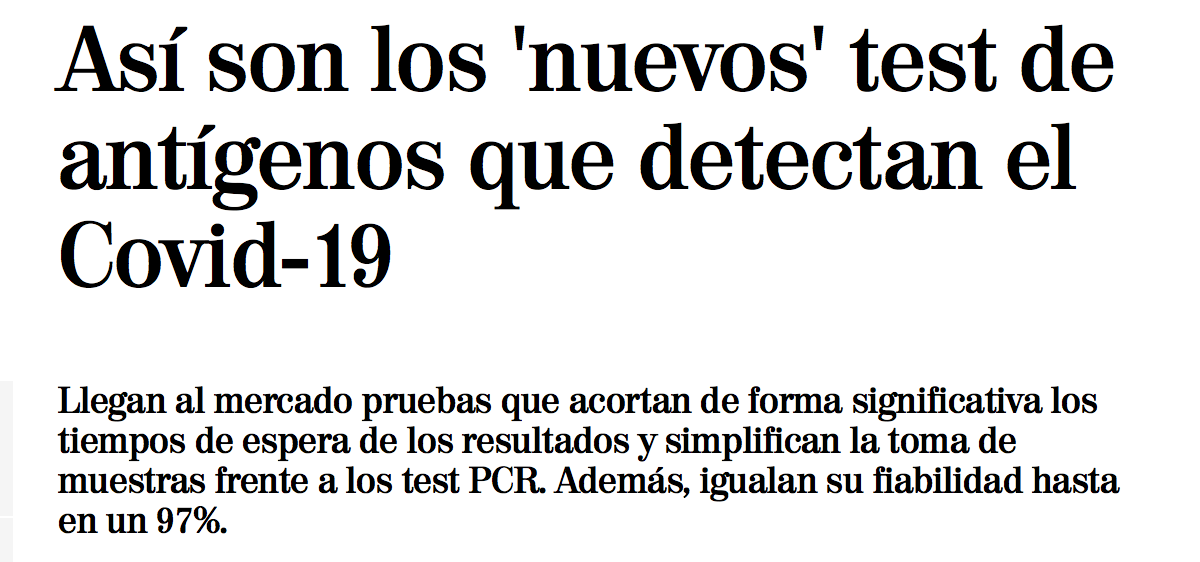
\includegraphics[width=0.6\linewidth]{INREMDN_files/figure-html/covidintro4} \end{center}

Estamos seguros de que aunque seáis recién llegados al grado de Medicina, con la que nos cayó encima en el 2020 este tipo de situaciones os es familiar, ¿verdad?

Por norma general, la información obtenida en este estudio clínico se habrá recogido sobre un conjunto más o menos pequeño de individuos, y se quiere determinar hasta qué punto se puede generalizar al total de la población mundial, o al menos a la población de nuestro entorno. La estadística es la que nos permite responder a esta cuestión.

Se ha definido estadística de muchas maneras. La que más nos gusta, y que entronca con la situación que acabamos de explicar, es que

\begin{quote}
La \textbf{estadística} es la ciencia que permite adquirir conocimiento generalizable a partir de datos.
\end{quote}

Una definición en la que apenas sobran palabras:

\begin{itemize}
\tightlist
\item
  En estadística, siempre se empieza obteniendo unos \textbf{datos} sobre un grupo (relativamente pequeño) de individuos de una población. Bueno, en realidad, no se empieza obteniendo los datos, sino planificando cuidadosamente cómo se van a obtener, pero todo forma parte de la ``obtención'' de los datos.
\item
  Se \textbf{generaliza la información} que se ha obtenido sobre este grupo de personas al total de la población.
\item
  Y no se trata de trucos de magia adivinatoria, sino de una \textbf{ciencia} cuya metodología ha sido validada por medio de demostraciones matemáticas o, en el peor de los casos, mediante simulaciones numéricas (el equivalente en matemáticas de los experimentos en las otras ciencias).
\end{itemize}

\begin{figure}

{\centering 
\includegraphics[width=0.8\linewidth]{INREMDN_files/figure-html/gaturro} 

}

\caption{Gaturro ((c) Nick) y la estadística.}\label{fig:gaturro}
\end{figure}

Así pues, la situación de partida a la hora de aplicar técnicas estadísticas es que disponemos de un conjunto de datos que describen algunas características de un grupo de individuos. El análisis estadístico de estos datos puede ser entonces de dos tipos básicos:

\begin{itemize}
\item
  \textbf{Análisis descriptivo}, cuando nuestro objetivo sea simplemente resumir, representar y explicar los datos concretos de los que disponemos. La \textbf{estadística descriptiva} es el conjunto de técnicas que se usan con este fin.
\item
  \textbf{Análisis inferencial}, si nuestro objetivo es deducir (\textbf{inferir}), a partir de estos datos, información significativa sobre el total de la población de interés. Las técnicas que se usan en este caso forman la \textbf{estadística inferencial}.
\end{itemize}

\begin{figure}

{\centering 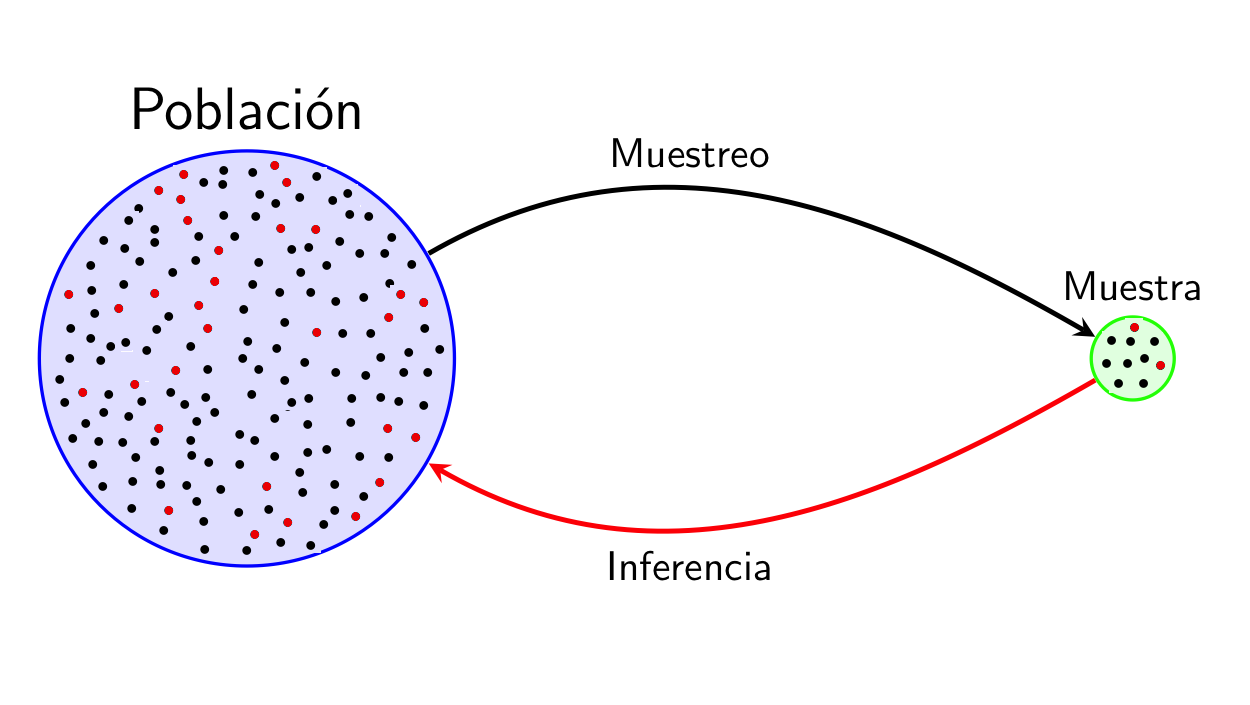
\includegraphics[width=0.8\linewidth]{INREMDN_files/figure-html/EstInf} 

}

\caption{Estadística inferencial.}\label{fig:estinf}
\end{figure}

Ambos tipos de análisis están relacionados. Por un lado, porque es conveniente (obligatorio, en nuestra opinión) empezar cualquier análisis inferencial dando un vistazo a los datos que se usarán. Por otro, porque muchas técnicas descriptivas permiten estimar propiedades de la población de la que se ha extraído la muestra. Por citar un ejemplo, la media aritmética de las alturas de un grupo de individuos nos da un valor más o menos representativo de sus alturas, pero también sirve para \emph{estimar} la altura media de los individuos de la población total.

La estadística inferencial entra en juego cuando se quiere obtener información sobre una población y no se puede acceder a todos sus integrantes. Si por ejemplo queremos conocer la altura media de los estudiantes matriculados en esta asignatura de la UIB en este curso, en principio no necesitamos para nada la estadística inferencial. Sois pocos, os mediríamos a todos y calcularíamos la media. En todo caso, usaríamos técnicas de estadística descriptiva para arropar este valor representando la distribución de vuestras alturas de manera adecuada.

Pero si quisiéramos conocer la altura media de los mallorquines de 18 años, sería muy complicado medirlos a todos. Entonces, lo que haríamos sería tomar una muestra representativa de esta población, medirlos y a partir de sus alturas estimar dicha altura media. Naturalmente, lo más seguro es que de esta manera no obtuviéramos el valor exacto de la altura media de los mallorquines de 18 años, nos tendríamos que conformar con obtener una aproximación dentro de un cierto margen de error y determinar la probabilidad de acertar con nuestra estimación y este margen de error. La estadística inferencial es la que nos permite acotar el error que podamos haber cometido y calcular la probabilidad de cometerlo, incluyendo la metodología que tendríamos que haber usado para tomar la muestra en primer lugar.

Hace más de 80 años, la prestigiosa revista médica \emph{The Lancet} ya avisaba en \href{https://www.sciencedirect.com/science/article/abs/pii/S0140673600865708}{un editorial titulado ``Matemáticas y medicina''} que muchos de los problemas en medicina son de estadística. Nos encanta la frase (a partir de la segunda línea del fragmento mostrado en la Figura \ref{fig:lancet2}): ``Los métodos estadísticos sencillos son mucho más de nuestra incumbencia que muchas de las cosas que nos obligan a estudiar en los seis largos años del currículo de Medicina''.

\begin{figure}

{\centering 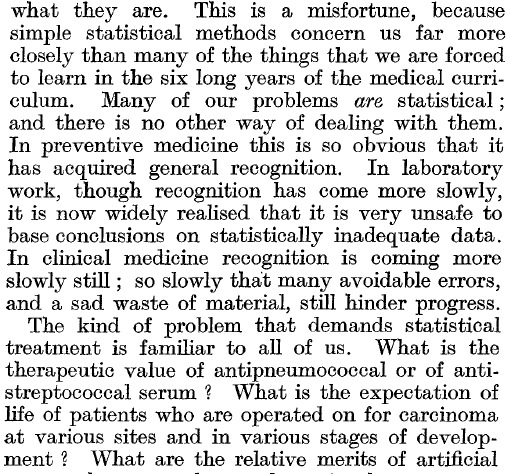
\includegraphics[width=0.5\linewidth]{INREMDN_files/figure-html/lancet2} 

}

\caption{Fragmento del editorial "Matemáticas y medicina" de *The Lancet* (2 de enero de 1937).}\label{fig:lancet2}
\end{figure}

En los últimos años, la necesidad de su conocimiento se ha reforzado con el auge de la \textbf{Medicina Basada en la Evidencia}. No vamos ahora a entrar en detalle sobre este enfoque de la medicina, porque seguro que os lo van a explicar en otras asignaturas mucho mejor de lo que lo haríamos aquí. Pero al menos hay que tener presente que su objetivo es \textbf{tomar decisiones médicas en base a la mejor evidencia científica disponible}. La evaluación de la evidencia disponible se tiene que basar en dos Es: en la \textbf{E}xperiencia del médico y en la \textbf{E}stadística. La segunda \textbf{E} se debe a que la mayoría de estudios médicos fundamentan sus conclusiones por medio de la estadística. Ya sabéis, usan la estadística para generalizar lo observado sobre los sujetos de una muestra a toda una población. Por tanto, para evaluar la fuerza de la evidencia obtenida en los estudios que consultéis a la hora de tomar una decisión, os serán necesarios unos mínimos conocimientos de estadística. Tendréis que ser capaces, por ejemplo, de discernir si el estudio se ha llevado a cabo correctamente, si el análisis de los datos se ha realizado de manera correcta, si las conclusiones a las que han llegado sus autores están bien fundamentadas y hasta qué punto son válidas en el caso clínico concreto que os ocupe.

Pues eso, el objetivo de esta asignatura es que adquiráis algunos de estos mínimos conocimientos de estadística.

\hypertarget{estudios-muxe9dicos}{%
\chapter{Estudios médicos}\label{estudios-muxe9dicos}}

Un \textbf{estudio} es un proceso cuyo objetivo es obtener evidencia empírica sobre alguna cuestión. En el caso de los estudios \textbf{médicos} que nos ocupan en este curso, esta cuestión es, naturalmente, sobre algún aspecto de la salud de las personas: la efectividad de un tratamiento, la precisión de un test diagnóstico, las causas de una enfermedad, algún tema de salud pública\ldots{}

\begin{figure}

{\centering 
\includegraphics[width=0.8\linewidth]{INREMDN_files/figure-html/anuncis} 

}

\caption{Estudios médicos.}\label{fig:anuncis}
\end{figure}

\hypertarget{sec:pasos}{%
\section{Pasos de un estudio médico}\label{sec:pasos}}

Para ir calentando motores, vamos a describir brevemente la estructura habitual de un estudio médico, y lo ilustraremos con el artículo \href{https://www.sciencedirect.com/science/article/pii/S0025775316305024}{``Marcha nórdica para prevención cardiovascular en pacientes con cardiopatía isquémica crónica o síndrome metabólico''} (C. Vehí \emph{et al},\footnote{Este \emph{et al} significa ``y otros'' y se utiliza para no dar toda la lista de autores de un artículo.} \emph{Medicina Clínica} 147 (2016), pp.~537-539) que convendría que fuerais consultando en paralelo a esta sección.

En un estudio médico por norma general se llevan a cabo los pasos siguientes:

\begin{enumerate}
\def\labelenumi{\arabic{enumi}.}
\item
  Se definen los \textbf{objetivos} de la investigación. En este primer paso,

  \begin{itemize}
  \tightlist
  \item
    Se describe la hipótesis general que se quiere investigar.
  \item
    Se concretan los objetivos específicos dentro de este marco general.
  \end{itemize}

  En el artículo que estamos siguiendo a modo de ejemplo:

  \begin{itemize}
  \tightlist
  \item
    La hipótesis general es que el ejercicio físico es efectivo en la prevención de riesgos cardiovasculares.
  \item
    El objetivo específico es determinar si la marcha nórdica reduce los factores de riesgo cardiovascular en los individuos del área sanitaria mediterránea.
  \end{itemize}
\item
  Se investigan los \textbf{antecedentes} sobre los objetivos específicos: ¿Qué se sabe sobre el tema?

  En nuestro ejemplo, los autores recogen algunos beneficios generales de la marcha nórdica y luego afirman que ``no hay datos de esta modalidad de ejercicio en el ámbito médico de la población mediterránea''.
\item
  Se \textbf{planifica} cómo se van a recoger los datos.

  En nuestro ejemplo, encontraréis el detalle de este punto en el apartado ``Material y métodos'' del artículo: diseño del estudio, criterios de inclusión de los participantes, actividad que tenían que realizar los participantes y cómo se recogieron los datos.
\item
  Se ejecuta el plan trazado y se \textbf{recogen} los datos.
\item
  Se \textbf{analizan} los datos.

  En nuestro ejemplo, los resultados de este análisis se recogen básicamente en la Tabla 2 del artículo.
\item
  Se extraen \textbf{conclusiones}.

  En nuestro ejemplo, las encontraréis en el apartado ``Discusión y conclusiones'' del artículo. Básicamente, los autores concluyen que ``Un programa de marcha nórdica es factible en el sistema sanitario público y puede ser útil para mejorar el control de los factores de riesgo cardiovascular''.
\item
  Se \textbf{publican} los resultados.

  Pues eso, los resultados del estudio de nuestro ejemplo se publicaron en el artículo que estamos comentando.
\end{enumerate}

Es un buen momento para que volváis al artículo y observéis su estructura, típica de los artículos en ciencias experimentales. Se trata de la estructura \textbf{IMRyD}, acrónimo de:

\begin{enumerate}
\def\labelenumi{\arabic{enumi}.}
\item
  \textbf{Introducción}, donde se recogen los pasos 1 y 2 del proceso anterior.
\item
  \textbf{Metodología} (``Material y métodos'', en este artículo concreto), donde se detallan los pasos 3 y 4.
\item
  \textbf{Resultados}, donde se explica el análisis de los datos y los resultados ``numéricos'' del mismo, sin extraer conclusiones aún (en plan ``obtuvimos esto, esto, esto y esto'').
\item
  \textbf{Discusión} (``Discusión y conclusiones'', en este artículo concreto), donde se completa el análisis de los datos, se extraen las conclusiones y se discute su alcance.
\end{enumerate}

El artículo científico además tiene otras dos partes muy importantes:

\begin{itemize}
\item
  El \textbf{Resumen} (\emph{Abstract}) al principio, describiendo lo más relevante de cada una de las cuatro partes centrales del artículo. Este resumen está relacionado con el último paso del proceso de investigación, la publicación de resultados, ya que en la mayoría de los casos es lo único que leemos, entrando solo en el detalle del artículo si, tras la lectura del resumen, decidimos que nos interesa de verdad.
\item
  La \textbf{Bibliografía} al final, relacionada en parte con el paso 2 (los antecedentes).
\end{itemize}

\begin{figure}

{\centering 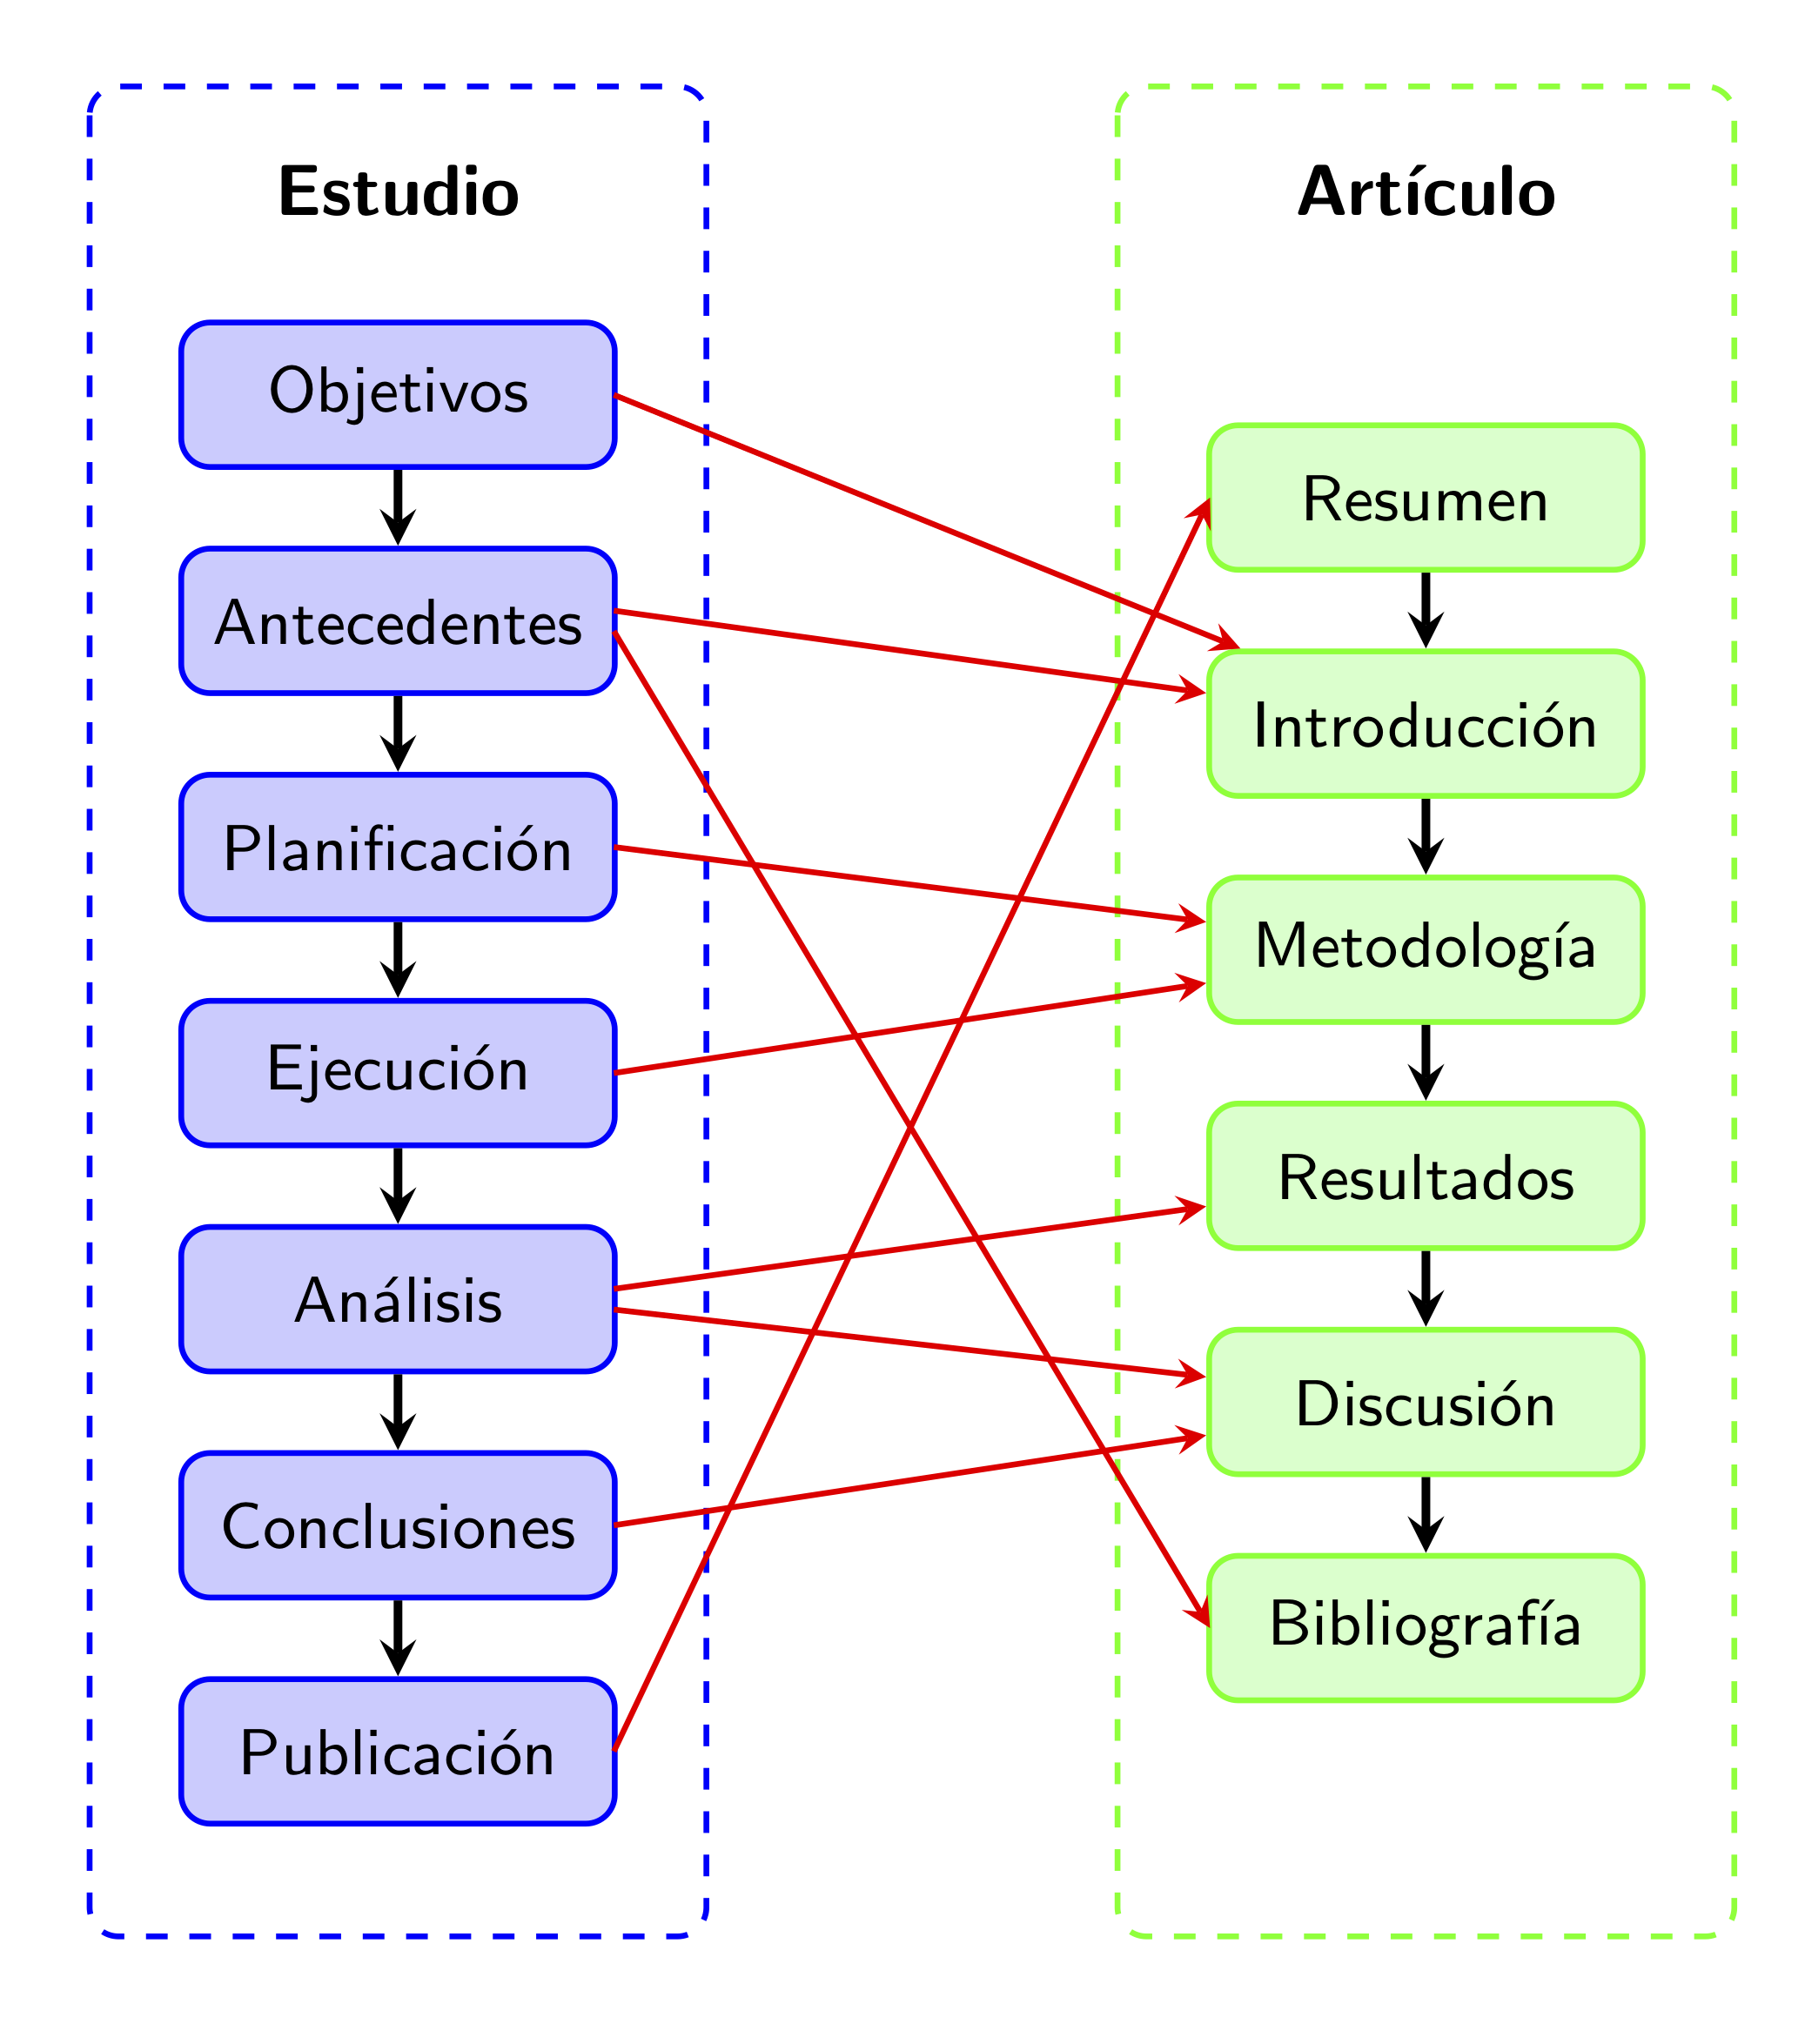
\includegraphics[width=0.8\linewidth]{INREMDN_files/figure-html/pasosvsarticle} 

}

\caption{Correspondencia entre los pasos de un estudio y la estructura IMRyD de un artículo científico.}\label{fig:pasosvsarticle}
\end{figure}

\hypertarget{algunos-calificativos-para-los-estudios-muxe9dicos}{%
\section{Algunos calificativos para los estudios médicos}\label{algunos-calificativos-para-los-estudios-muxe9dicos}}

Podemos clasificar los estudios médicos de diferentes maneras:

\begin{itemize}
\item
  Según su \textbf{alcance}:

  \begin{itemize}
  \item
    \textbf{Descriptivos}: Se limitan a describir las características de un grupo de individuos.
  \item
    \textbf{Analíticos}: Intentan inferir asociaciones para el total de la población (de tipo causa/efecto, antecedente/desenlace, \ldots).
  \end{itemize}

  Por ejemplo:

  \begin{itemize}
  \tightlist
  \item
    ``A cinco pacientes con la enfermedad X les hemos administrado el tratamiento A y tres estaban curados a los 8 días de iniciar el tratamiento. Y punto.'': \textbf{Descriptivo}.
  \item
    ``Hemos dividido un grupo de pacientes con la enfermedad X en dos grupos. A unos les hemos administrado el tratamiento A y a los otros el tratamiento B. Los tratados con A han tenido una tasa de curación a 8 días vista mucho más alta que los tratados con B. Llegamos a la conclusión que el tratamiento A es más efectivo que el B para los enfermos de X.'': \textbf{Analítico}.
  \end{itemize}
\item
  Según el \textbf{papel jugado por el investigador}:

  \begin{itemize}
  \item
    \textbf{Observacionales}: El investigador se limita a recoger datos, sin ejercer ninguna influencia planificada sobre los acontecimientos que generan estos datos.
  \item
    \textbf{Intervencionista}: El investigador influye de manera planificada en los acontecimientos que generan los datos que recoge.
  \end{itemize}

  Por ejemplo:

  \begin{itemize}
  \tightlist
  \item
    ``Hemos recogido datos de todos los pacientes con la enfermedad X en nuestro hospital durante un año y anotado qué tratamiento se les ha administrado. Los tratados con A han presentado una tasa de curación a 8 días vista más alta que los tratados con B.'': \textbf{Observacional}.
  \item
    ``Hemos dividido al azar un grupo de pacientes con la enfermedad X en dos grupos del mismo tamaño. A unos les hemos administrado el tratamiento A y a los otros el tratamiento B. Los tratados con A han tenido una tasa de curación a 8 días vista más alta que los tratados con B.'': \textbf{Intervencionista}.
  \end{itemize}
\item
  Según el \textbf{lapso de tiempo} sobre el que se recoge la información:

  \begin{itemize}
  \item
    \textbf{Transversales}: Se recoge información sobre un solo momento.
  \item
    \textbf{Longitudinales}: Se recoge información sobre varios momentos de tiempo y se estudian los cambios producidos entre los mismos.

    A su vez, estos últimos suelen dividirse en:

    \begin{itemize}
    \item
      \textbf{Prospectivos}: Se recoge información en un momento concreto (normalmente, al inicio del estudio) y en momentos posteriores.
    \item
      \textbf{Retrospectivos}: Se recoge información en un momento concreto (de nuevo, normalmente, al inicio del estudio) y sobre momentos anteriores.
    \end{itemize}
  \end{itemize}

  Por ejemplo:

  \begin{itemize}
  \tightlist
  \item
    ``Hoy hemos tomado una muestra de 100 estudiantes de la UIB y les hemos hecho un test de COVID-19.'' \textbf{Transversal}.
  \item
    ``Hoy hemos tomado un grupo de enfermos de COVID-19 y les vamos a hacer un seguimiento para estudiar si la evolución de la enfermedad depende del Índice de Masa Corporal del enfermo en el momento del diagnóstico.'' \textbf{Longitudinal prospectivo}.
  \item
    ``Hoy hemos tomado un grupo de enfermos de COVID-19 con síntomas leves y un grupo con síntomas muy graves, y les hemos preguntado por su hábito de uso de mascarilla en las últimas semanas.'' \textbf{Longitudinal retrospectivo}.
  \end{itemize}
\end{itemize}

\begin{example}
\protect\hypertarget{exm:unnamed-chunk-15}{}\label{exm:unnamed-chunk-15}

El estudio sobre la marcha nórdica de la sección anterior es:

\begin{itemize}
\item
  \textbf{Analítico}, puesto que su objetivo es inferir los efectos de la marcha nórdica en los factores de riesgo cardiovascular para las personas del área sanitaria mediterránea, no solo describir qué les pasó a los 23 individuos que participaron en el estudio.
\item
  \textbf{Longitudinal prospectivo}, puesto que se compararon datos tomados en el momento de iniciar el estudio y al cabo de un año.
\item
  \textbf{Intervencionista}, puesto que los investigadores influyeron en el comportamiento de los participantes al hacerles realizar unas sesiones semanales de marcha nórdica con el fin de estudiar su efecto.
\end{itemize}

\end{example}

\begin{rmdnote}
Si los investigadores hubieran recetado una terapia de marcha nórdica a los participantes porque, según su criterio médico, lo necesitaban y no porque participaban en un estudio, este no hubiera sido intervencionista, sino observacional. Para que sea intervencionista la ``intervención'' del investigador ha de estar motivada por el estudio.
\end{rmdnote}

\begin{rmdexercici}
``Para estudiar si la vacunación reduce el riesgo de síntomas graves en la COVID-19, hemos tomado un grupo de infectados y hemos anotado por un lado la gravedad de sus síntomas y por otro lado si están vacunados con la pauta completa, vacunados a medias o no vacunados.'' ¿Longitudinal o transversal?
\end{rmdexercici}

\begin{rmdexercici}
Combinando los tipos de estudio según el papel jugado por el investigador y según el lapso de tiempo sobre el que se recoge la información, tenemos estudios:

\begin{itemize}
\tightlist
\item
  Observacionales transversales
\item
  Observacionales prospectivos
\item
  Observacionales retrospectivos
\item
  Intervencionistas transversales
\item
  Intervencionistas prospectivos
\item
  Intervencionistas retrospectivos
\end{itemize}

Acabamos de ver que hay estudios intervencionistas prospectivos. ¿Los hay de las otras cinco clases de estudios de esta lista, o hay algún par de características que es imposible que se den simultáneamente?
\end{rmdexercici}

En las siguientes secciones discutimos con más detalle los tipos más básicos de estudios médicos, anotados en la Figura \ref{fig:estudisgraf}.

\begin{figure}

{\centering 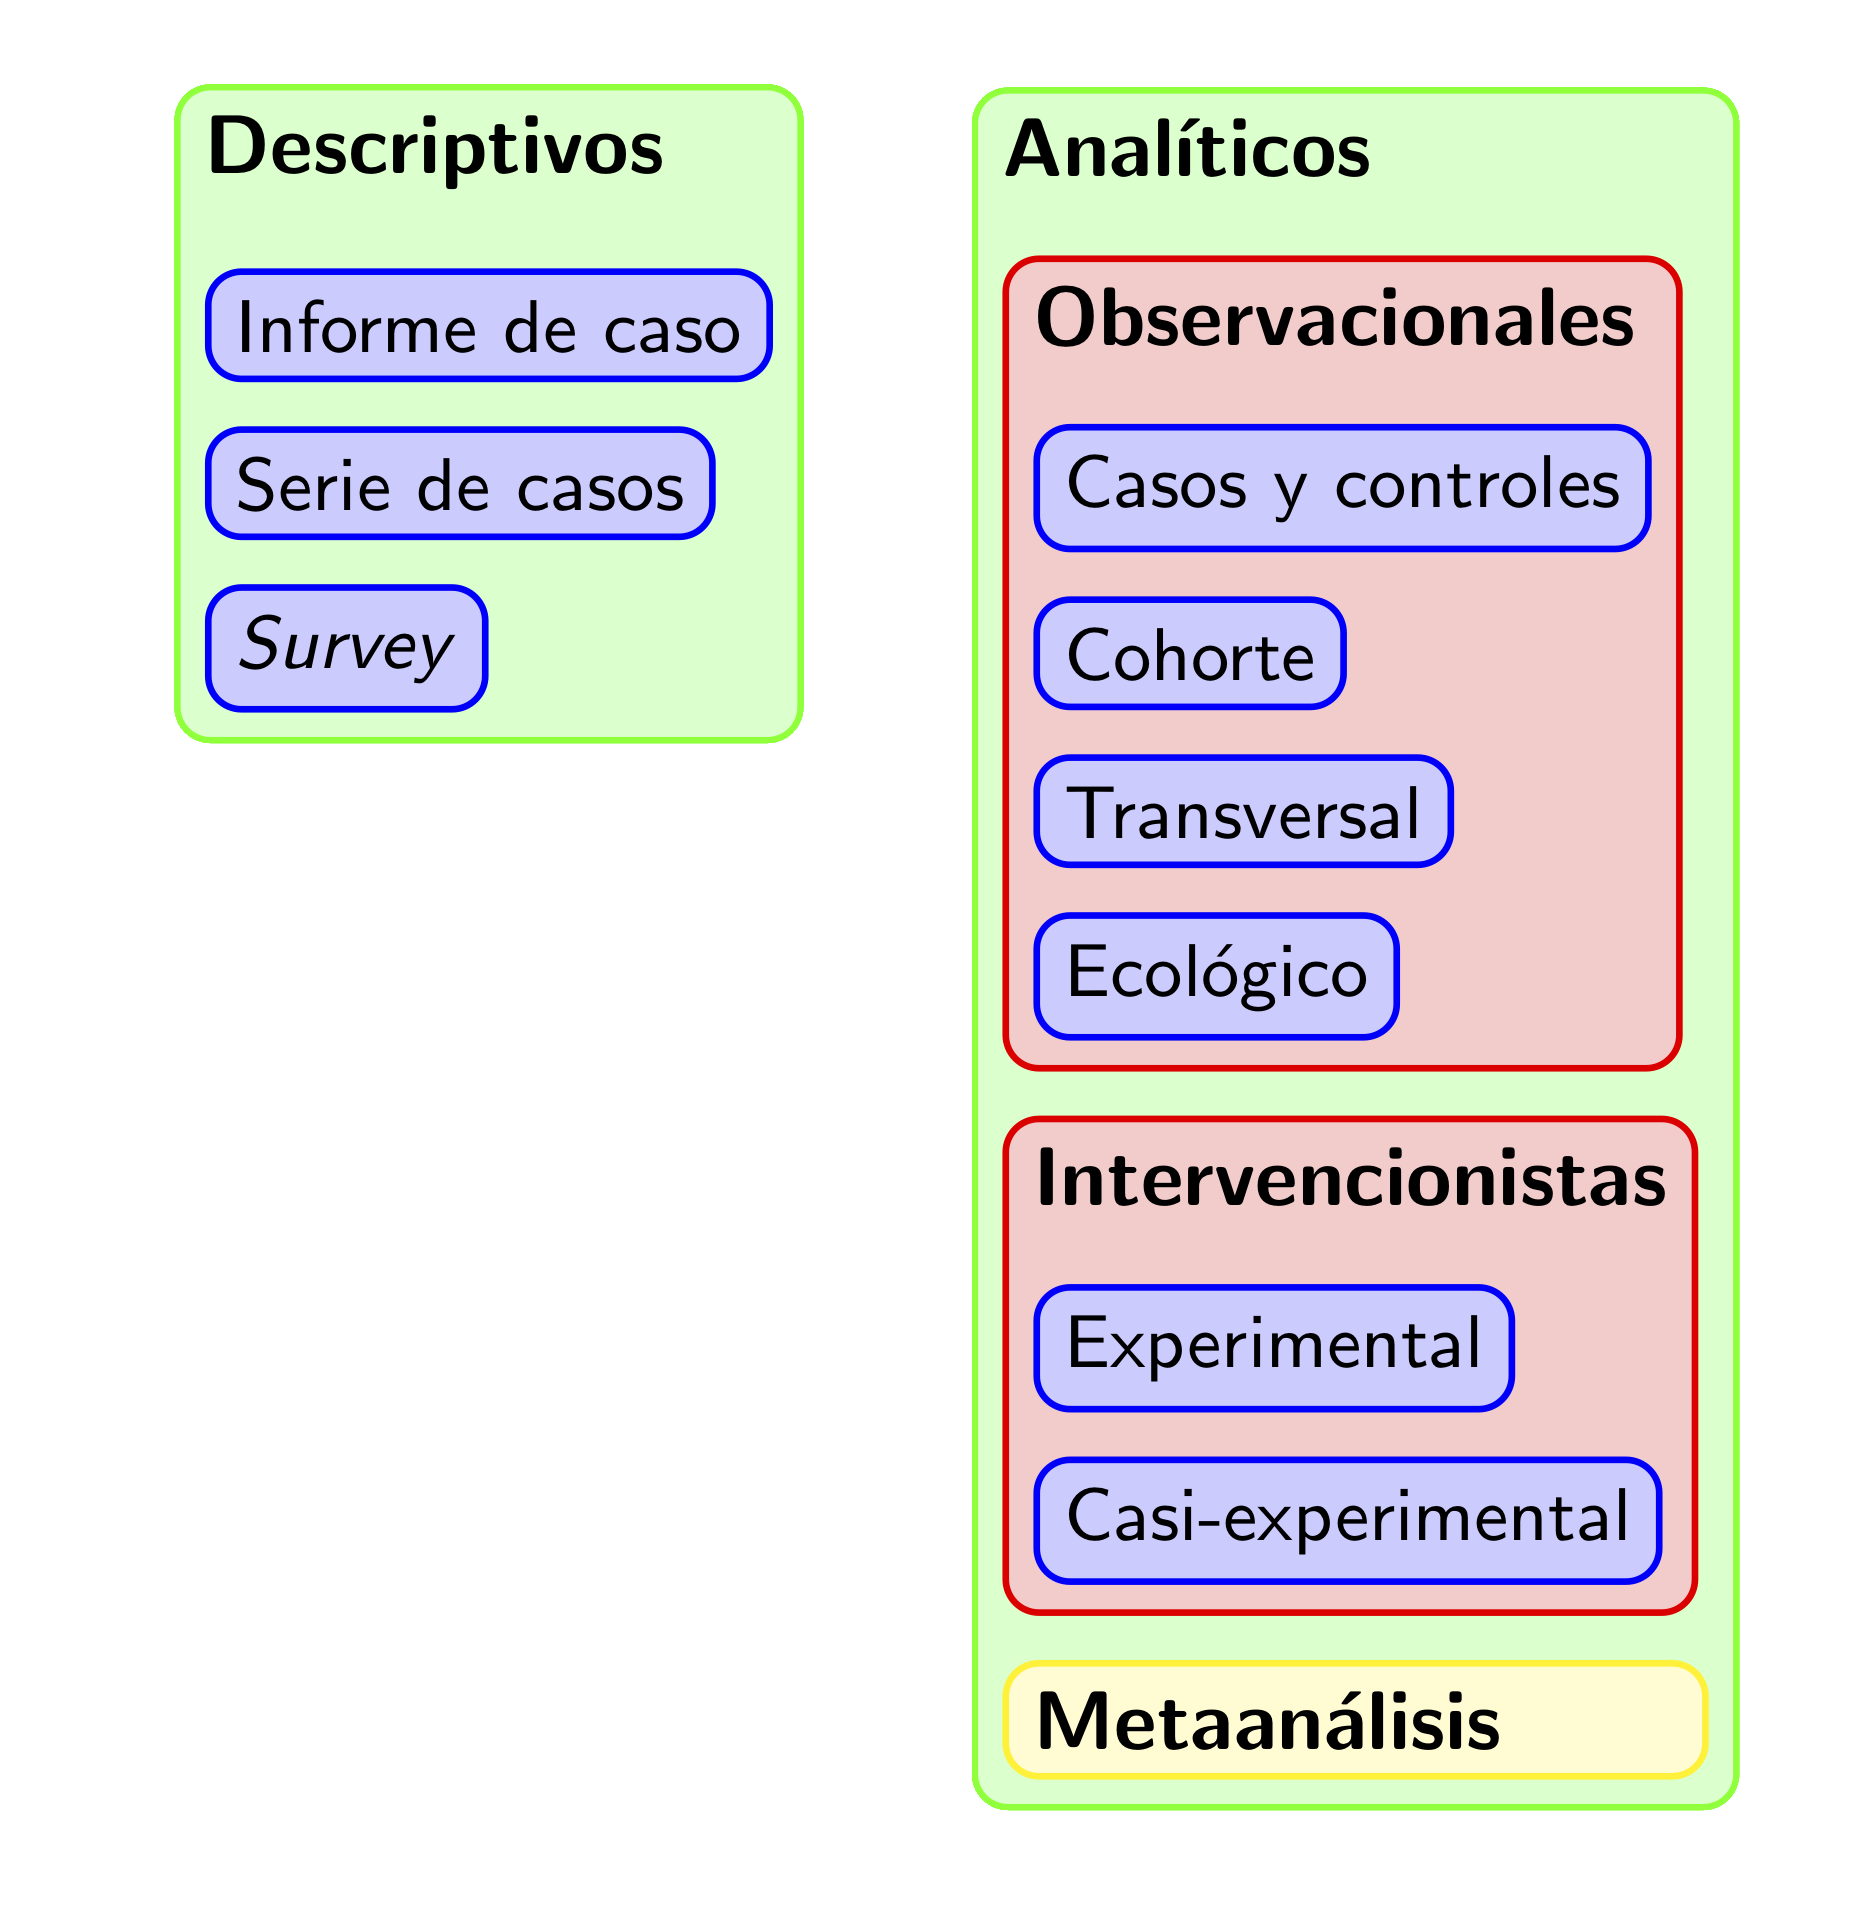
\includegraphics[width=0.8\linewidth]{INREMDN_files/figure-html/estudis} 

}

\caption{Tipos básicos de estudios médicos.}\label{fig:estudisgraf}
\end{figure}

\hypertarget{estudios-descriptivos}{%
\section{Estudios descriptivos}\label{estudios-descriptivos}}

Los tres tipos principales de estudios descriptivos son:

\begin{itemize}
\item
  \textbf{Informe de caso}: La descripción detallada de un paciente.
\item
  \textbf{Serie de casos}: Descripción detallada de un conjunto pequeño de pacientes (pero más de uno, o sería un informe de \emph{un} caso) con algún problema de salud en común. La información se recoge por medio de sus historias clínicas y entrevistas clínicas.
\end{itemize}

\begin{rmdrecordau}
En el contexto de los estudios médicos, el término \textbf{casos} siempre refiere a sujetos enfermos, o con algún problema de salud.
\end{rmdrecordau}

\begin{itemize}
\tightlist
\item
  \textbf{Encuesta} (\emph{Survey}): Descripción de un conjunto ``grande'' de individuos con alguna característica en común. La información se recoge por medio de cuestionarios o entrevistas.
\end{itemize}

Recordad que los estudios descriptivos solo \textbf{describen} un sujeto o un conjunto de sujetos, sin pretender ir más allá. Aparte de su utilidad como anécdota (``¡Mira, a este esto le funcionó, vamos a probar a ver!'') y para alertar de nuevas enfermedades, sirven principalmente para identificar observaciones interesantes que merezcan ser investigadas.

\begin{example}
\protect\hypertarget{exm:origenesHIV}{}\label{exm:origenesHIV}Lo que más tarde se reconocería como la epidemia de SIDA se presentó en sociedad en unas primeras series de casos publicadas a principios de los años 1980. En ellos se describían casos de jóvenes homosexuales sanos que habían desarrollado enfermedades relacionadas con una deficiencia grave del sistema inmunitario, como por ejemplo infecciones oportunistas o el sarcoma de Kaposi (un tipo de cáncer de piel asociado a una infección vírica que hasta entonces solo se había detectado básicamente en ancianos de ascendencia judía o mediterránea y en jóvenes en África). Cuando el número de publicaciones de casos similares fue abrumador, se llevó a cabo un \href{https://www.acpjournals.org/doi/abs/10.7326/0003-4819-99-2-145}{estudio de casos y controles} (\emph{casos}: enfermos de lo que fuera esa enfermedad; \emph{controles}: personas sanas de características similares a los casos; explicaremos los estudios de casos y controles en la próxima sección) para determinar cuáles eran las características, hábitos, comportamientos etc. que tenían en común los enfermos y no compartían con los sanos.
\end{example}

\begin{example}
\protect\hypertarget{exm:diabetesSC}{}\label{exm:diabetesSC}El artículo \href{http://www.scielo.org.pe/pdf/rmh/v26n1/a02v26n1.pdf}{``Diabetes tipo 2 en niños. Serie de casos''} (H. Manrique-Hurtado \emph{et al}, \emph{Revista Médica Herediana} 26 (2015), pp.~5-9) es, como indica su título, un ejemplo típico de serie de casos. Se trata de una descripción detallada de las características de todos los niños y adolescentes diagnosticados de diabetes tipo 2 (DM2) en dos hospitales de Lima (Perú) entre 2008 y 2013. En total, se describen 32 sujetos de entre 8 y 19 años.

Entre otras características, se observó que, en el momento del diagnóstico, el 85\% de ellos presentaban acantosis pigmentaria (un transtorno de la piel); que un 17\% tenían cetoacidosis diabética (CAD), que suele ir asociada a diabetes tipo 1 y no 2; y que estos últimos presentaban todos una serie de características comunes, por ejemplo todos tenían acantosis pigmentaria.

Todas estas observaciones sirven para confirmar, o contradecir, observaciones realizadas en otros momentos u otros países sobre enfermos de DM2 en esta franja de edad. Además, plantean cuestiones sobre la DM2 en niños y adolescentes que pueden ser susceptibles de responderse mediante estudios analíticos. Por ejemplo: ¿Es la acantosis pigmentaria un síntoma frecuente de DM2 entre niños y adolescentes? ¿Presentar CAD y acantosis pigmentaria es más síntoma de DM2 que de DM1 entre niños y adolescentes?
\end{example}

\begin{example}
\protect\hypertarget{exm:surveycovid}{}\label{exm:surveycovid}En el estudio \href{https://journals.lww.com/jbjsjournal/Fulltext/2020/05200/Survey_of_COVID_19_Disease_Among_Orthopaedic.1.aspx}{``Survey of COVID-19 Disease Among Orthopaedic Surgeons in Wuhan, People's Republic of China''} (X. Guo \emph{et al}, \emph{The Journal of Bone and Joint Surgery} 102 (2020), pp.~847-854), se pasó un cuestionario a todos los cirujanos ortopédicos del área urbana de Wuhan (China) que no habían sido destinados específicamente a tratar enfermos de COVID-19. El objetivo era identificar cuántos habían tenido COVID-19 antes de finales de febrero de 2020 y recoger una serie de características de interés sobre ellos: sus síntomas, a cuánta gente contagiaron, su estado de salud previo al contagio, la distancia de su hospital al mercado mayorista de mariscos de Huanan (donde se cree que se inició la pandemia) etc. Se encontraron en total 24 infectados, y sus características se describen en el artículo mencionado.

Esta parte del estudio es descriptiva: una descripción de todos los casos de COVID-19 en un colectivo concreto. El estudio luego tuvo una segunda parte analítica que clasificaremos como \textbf{de casos y controles} en la próxima sección.
\end{example}

\begin{rmdromans}
Hemos dicho que una serie de casos describe un grupo pequeño de individuos, y que un \emph{survey} describe un grupo grande. En la serie de casos del Ejemplo \ref{exm:diabetesSC} se describieron 32 pacientes, y en el \emph{survey} (así es como lo clasifican sus autores en el título) del Ejemplo \ref{exm:surveycovid} solo 24 infectados. ¿32 es pequeño y 24 es grande?

¡Claro que no! La diferencia aquí está en cómo se obtuvo la información: por medio de historias clínicas en el estudio peruano y por medio de un cuestionario en el estudio chino. Además, en este segundo caso el cuestionario se pasó a 428 médicos, por lo que el número de pacientes ``descritos'' podría haber sido mucho mayor.
\end{rmdromans}

\hypertarget{sec:cyc}{%
\section{Estudios de casos y controles}\label{sec:cyc}}

En un \textbf{estudio de casos y controles}:

\begin{itemize}
\item
  Se toma un grupo de individuos con una enfermedad (los \textbf{casos}) y un grupo de individuos sin esta enfermedad (los \textbf{controles})
\item
  Se les compara \textbf{retrospectivamente} para encontrar diferencias en su exposición a factores de riesgo en el pasado.
\item
  Se determinan qué factores de riesgo fueron más frecuentes entre los casos que entre los controles.
\item
  Se infiere (mejor dicho, se estudia si se puede inferir) que, en la población general, la exposición a dichos factores está asociada a una mayor probabilidad de enfermar.
\end{itemize}

\begin{figure}

{\centering 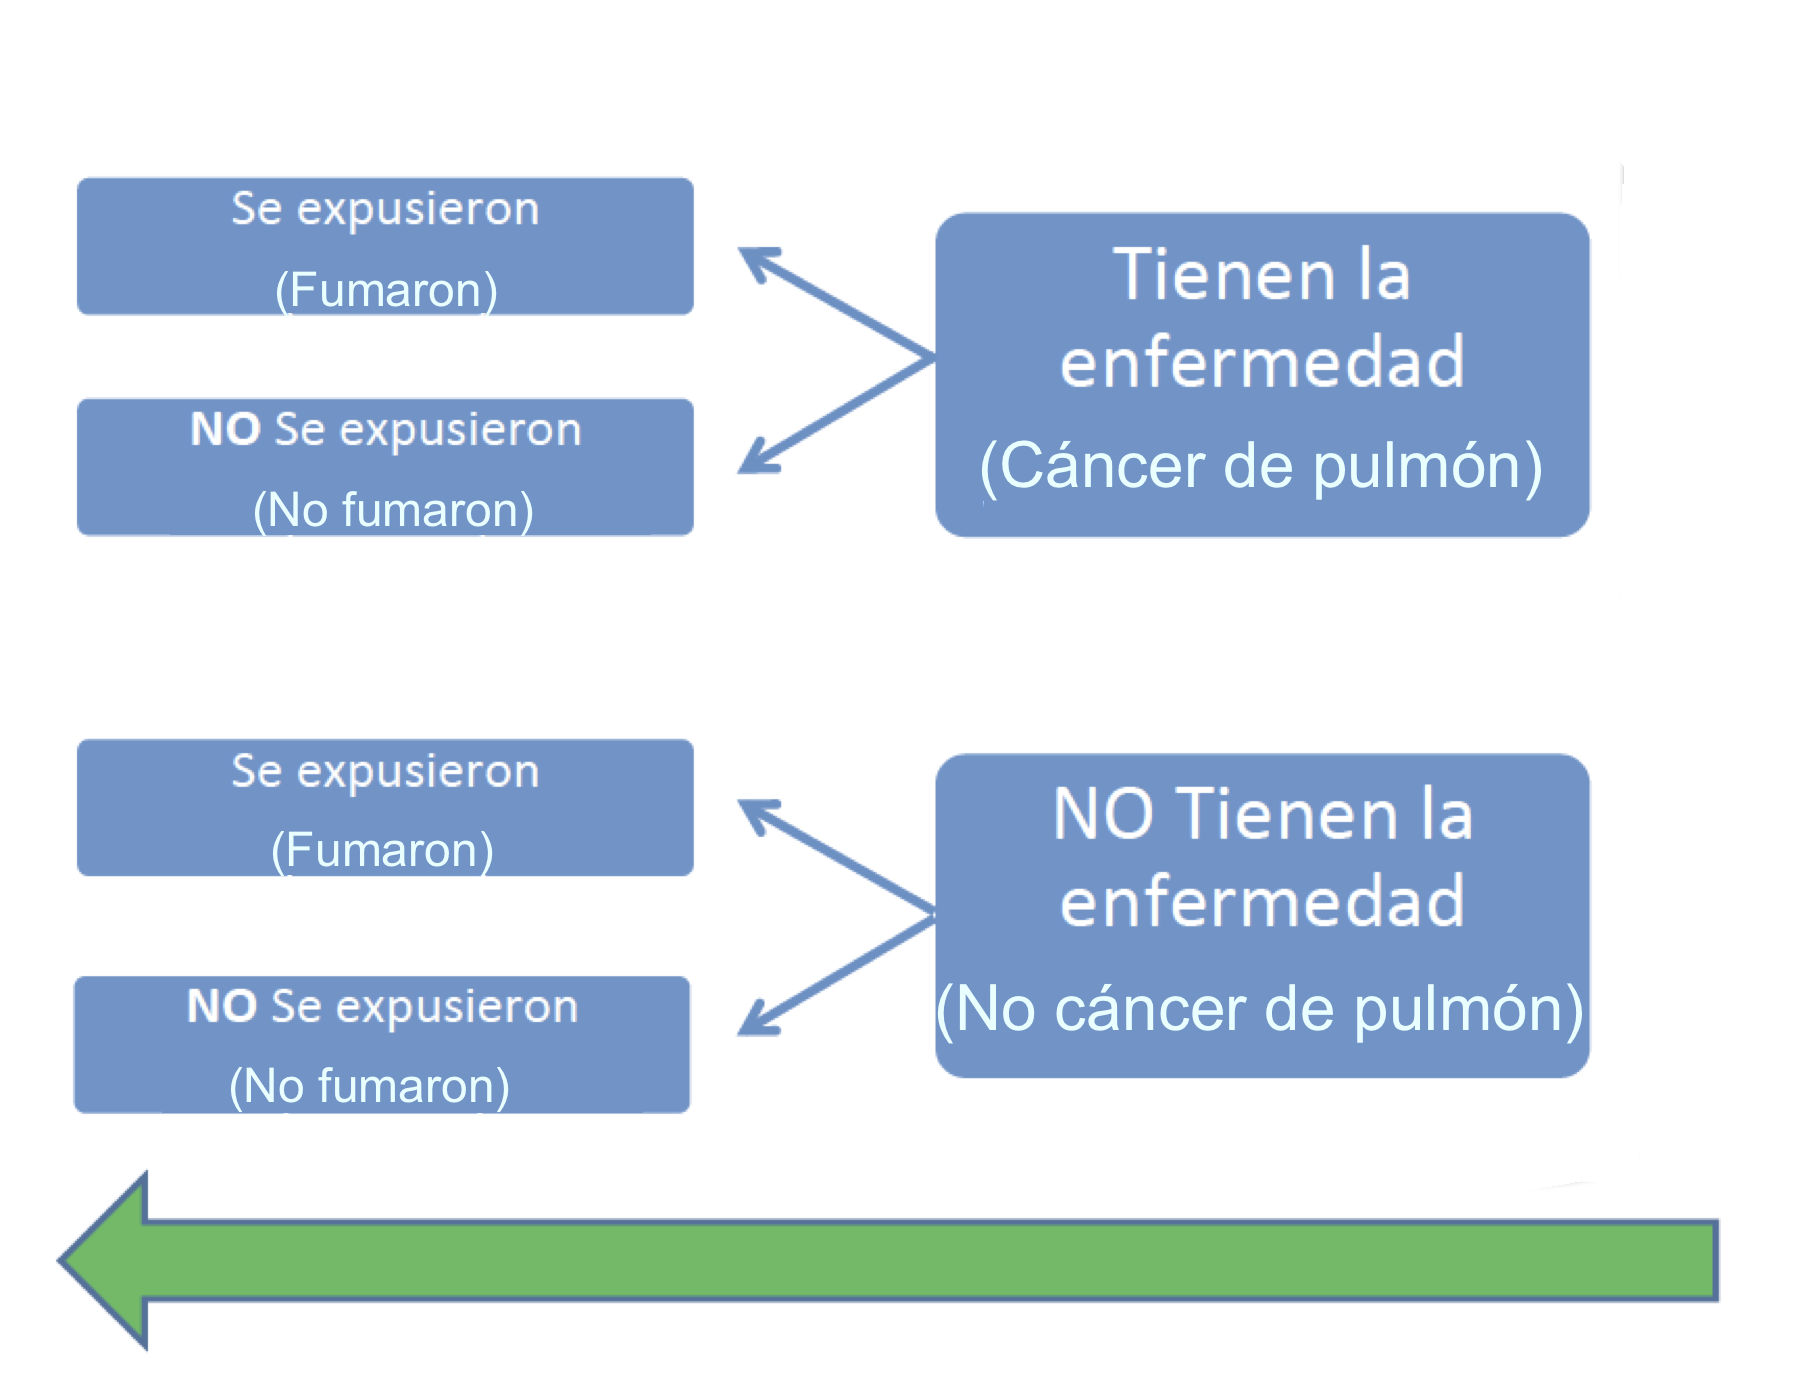
\includegraphics[width=0.8\linewidth]{INREMDN_files/figure-html/cataratas} 

}

\caption{Esquema del estudio de casos y controles del Ejemplo \\ref{exm:rubeola}.}\label{fig:cataratas}
\end{figure}

\begin{example}
\protect\hypertarget{exm:unnamed-chunk-21}{}\label{exm:unnamed-chunk-21}En \href{https://www.ncbi.nlm.nih.gov/pmc/articles/PMC2022425/}{uno de los primeros estudios de casos y controles}, R. Doll y A. Bradford Hill tomaron 1357 \textbf{casos} de hombres con cáncer de pulmón y 1357 \textbf{controles}, hombres con cáncer de otros tipos. Les preguntaron por el número medio diario de cigarrillos que habían fumado durante los 10 años anteriores al diagnóstico. Los resultados fueron los de la Figura \ref{fig:doll}, donde se observa una clara tendencia a ser más fumador entre los casos que entre los controles.
\end{example}

\begin{figure}

{\centering 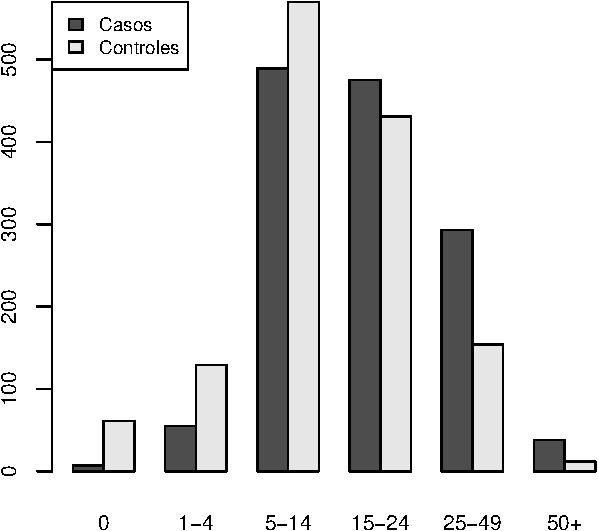
\includegraphics[width=0.5\linewidth]{INREMDN_files/figure-latex/doll-1} 

}

\caption{Consumo de tabaco en la muestra analizada por R. Doll y R. Bradford Hill en "Study of the Aetiology of Carcinoma of the Lung", *British Medical Journal* 2 (1952), pp. 1271–1286.}\label{fig:doll}
\end{figure}

Los estudios de casos y controles son:

\begin{itemize}
\item
  \textbf{Observacionales}, porque se recogen datos y se analizan sin influir en las características que se han medido.
\item
  \textbf{Analíticos}, puesto que el objetivo es deducir la asociación entre los factores de riesgo y la enfermedad a nivel poblacional.
\item
  \textbf{Longitudinales}, puesto que se analiza información sobre un período de tiempo, que va desde el momento en que los sujetos son declarados casos o controles hacia el pasado. Por lo tanto, son además \textbf{retrospectivos}.
\end{itemize}

Veamos un estudio de casos y controles más reciente.

\begin{example}
\protect\hypertarget{exm:tuberculosisCC}{}\label{exm:tuberculosisCC}En el estudio \href{https://www.scielo.br/scielo.php?pid=S1806-37132019000200205\&script=sci_arttext\&tlng=es}{``Tabaquismo y fracaso del tratamiento de la tuberculosis pulmonar. Un estudio de casos y controles''} (J. P. Aguilar \emph{et al}, \emph{Jornal Brasileiro de Pneumologia} 45.2 (2019), e20180359) se tomaron todos los pacientes que recibieron tratamiento contra la tuberculosis en una institución brasileña concreta entre 2007 y 2015 y que además satisfacían algunas restricciones extra (mayores de 15 años, sin diabetes ni SIDA\ldots). Se definieron como \textbf{casos} aquellos pacientes en los que el tratamiento fracasó (según unos criterios precisos) y como \textbf{controles} aquellos pacientes en los que tuvo éxito. En total fueron 50 casos y 234 controles.
\end{example}

\begin{center}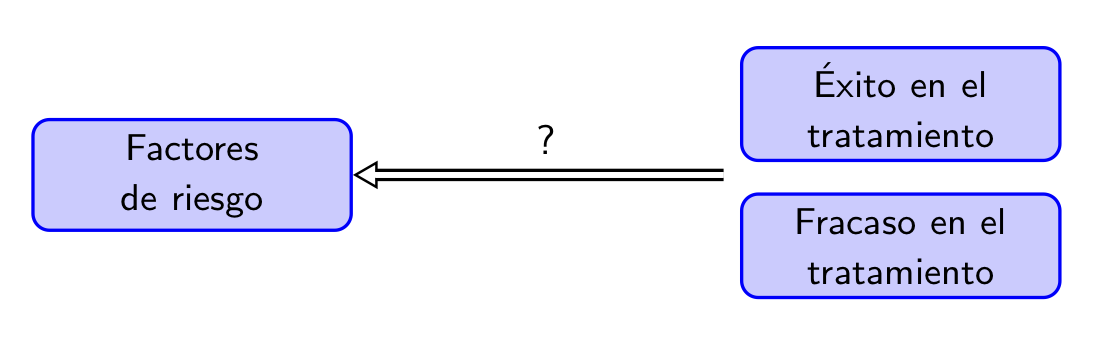
\includegraphics[width=0.8\linewidth]{INREMDN_files/figure-html/TB} \end{center}

Se analizaron un buen número de antecedentes que pudieran influir en el desenlace del tratamiento de la tuberculosis: sexo, edad, historial de fumador, historial de consumo de alcohol, salario etc. La única diferencia ``significativa'' que encontraron fue en el fumar: un 52\% de los casos eran fumadores en el momento del diagnóstico de la tuberculosis o lo habían sido antes, contra solo un 30\% de los controles. En cambio, por ejemplo, eran consumidores frecuentes de alcohol en el momento del diagnóstico de la tuberculosis o lo habían sido antes un 59\% de los casos y un 52\% de los controles, una diferencia que no fue lo suficientemente grande como para poder considerarla ``significativa''.

El adjetivo \textbf{significativo} (en realidad, \textbf{estadísticamente significativo}, pero por ahora omitiremos el adverbio ``estadísticamente'' para abreviar), que ha salido dos veces y hemos entrecomillado en el párrafo anterior, tiene un significado muy concreto en estadística, sobre el que volveremos más adelante en el curso. Por ahora lo tomaremos en el sentido intuitivo de \textbf{tan grande que sería muy raro que fuera casualidad, lo que nos hace sospechar que también hay diferencia en la población en general}. Por ejemplo:

\begin{itemize}
\item
  La diferencia entre el 52\% de fumadores entre los casos y el 30\% de fumadores entre los controles fue tan grande, que hubiera sido muy improbable si, en la población general, la proporción de fumadores entre los pacientes en los que el tratamiento fracasa fuera la misma que en los que tiene éxito.

  Esto nos lleva a concluir que la proporción de fumadores entre los individuos en los que el tratamiento de tuberculosis fracasa es mayor que entre aquellos en los que tiene éxito.
\item
  La diferencia entre el 59\% de consumidores frecuentes de alcohol entre los casos y el 52\% entre los controles no fue lo bastante grande como para ser muy improbable si, en la población general, la proporción de consumidores frecuentes de alcohol entre los casos fuera la misma que entre los controles.

  En este caso, no tenemos base para concluir que la proporción de consumidores frecuentes de alcohol entre los individuos en los que el tratamiento de tuberculosis fracasa sea mayor que entre aquellos en los que tiene éxito.
\end{itemize}

En este estudio, los números de casos y controles no se prefijaron en su diseño, sino que se tomaron ``los que encontraron'' en un grupo de individuos. Por lo tanto, en principio, su composición en casos y controles refleja la de la población. Diremos en casos como este que el grupo de sujetos analizados forman una \textbf{muestra transversal} de la población.

\begin{rmdcaution}
Id con cuidado, que el adjetivo transversal ya ha salido con dos significados diferentes (y aún habrá un tercero):

\begin{itemize}
\tightlist
\item
  Estudio \textbf{transversal} en el tiempo: Se recogen datos sobre un solo momento.
\item
  Muestra \textbf{transversal}: Una muestra cuya composición en diferentes clases (por ejemplo, en casos y controles) no está prefijada de ninguna manera, y por lo tanto esperamos que sea representativa de la población.
\end{itemize}
\end{rmdcaution}

Esto no siempre es así, y a veces se toman números concretos, o al menos relacionados entre si, de casos y controles: tantos casos como controles, el doble de controles que de casos\ldots{} Llamaremos a una muestra de este estilo \textbf{estratificada} (Sección \ref{sec:estr}). Es importante distinguir las muestras transversales de las estratificadas, porque en un estudio de casos y controles hay que tener en cuenta el tipo de muestra que se ha tomado a la hora de realizar el análisis estadístico de los datos y extraer conclusiones.

Por ejemplo, tal y como se tomó la muestra en el estudio anterior, tiene sentido calcular la proporción de tuberculosos de la muestra sobre los que el tratamiento tuvo éxito y usar esta proporción para estimar la tasa de éxito del tratamiento entre los tuberculosos en general. En cambio, imaginad que se hubieran tomado a propósito el mismo número de casos que de controles. Ahora la proporción de tuberculosos tratados con éxito en la muestra sería ``artificial'', y no se podría usar para inferir información sobre la tasa de éxito del tratamiento.

Veamos dos ejemplos de estudios de casos y controles con muestras estratificadas.

\begin{example}
\protect\hypertarget{exm:CAPUA}{}\label{exm:CAPUA}Considerad el estudio \href{https://www.sciencedirect.com/science/article/pii/S0025775317300362}{``Efecto del alcohol y sus metabolitos en el cáncer de pulmón: estudio CAPUA''} (S. M. Álvarez-Avellón \emph{et al}, \emph{Medicina Clínica} 148 (2017), pp.~531-538). En él se incluyeron 876 \textbf{casos}, enfermos de cáncer de pulmón ingresados en una serie de hospitales asturianos entre 2000 y 2010, y 840 \textbf{controles}, pacientes que fueron atendidos en los mismos hospitales que los casos por patologías no relacionadas con ningún factor de riesgo conocido de cáncer de pulmón. Se les entrevistó para conocer sus hábitos alimentarios y de consumo de alcohol y tabaco y se les realizó un análisis genético de los polimorfismos de algunos genes que codifican enzimas participantes en el metabolismo del alcohol y el folato (un tipo de vitamina B). Copiamos algunas conclusiones:
\end{example}

\begin{itemize}
\item
  Un consumo de alcohol de 0.1-9.9 g/día disminuye el riesgo de cáncer de pulmón, aunque la diferencia no es significativa.
\item
  Un consumo de alcohol de ≥ 30 g/día y de tabaco de ≥ 36 paquetes/año aumenta significativamente el riesgo de cáncer de pulmón.
\item
  Un consumo de alcohol de 10-29.9 g/día en individuos portadores del alelo \emph{ADH1B 48His} aumenta de manera significativa el riesgo de cáncer de pulmón.
\end{itemize}

\begin{example}
\protect\hypertarget{exm:surveycovid2}{}\label{exm:surveycovid2}Volvamos al Ejemplo \ref{exm:surveycovid}. Una vez identificados los 24 cirujanos que habían tenido la COVID-19, se escogieron al azar 48 cirujanos (dos por cada enfermo) que \textbf{no} habían tenido (aún) la COVID-19 de entre los que habían respondido el cuestionario. Se compararon entonces los datos sobre la exposición previa a algunos factores de riesgo entre ambos grupos: grado de fatiga, horas de sueño, uso de mascarilla al tratar con pacientes, etc. Esta segunda parte del estudio es claramente de \textbf{casos} (cirujanos que habían tenido COVID-19) y \textbf{controles} (cirujanos que no habían tenido COVID-19).
\end{example}

En este estudio chino se puede observar la gran ventaja de un estudio de casos y controles sobre un estudio descriptivo: el disponer del grupo de control para poder comparar. Por ejemplo, resultó que un 58.7\% de los cirujanos que habían tenido COVID-19 no habían recibido formación específica reciente sobre control de infecciones. Son muchos, pero esta cifra aislada no sirve para concluir que no haber recibido formación específica reciente sobre control de infecciones aumenta el riesgo de contraer la COVID-19. A lo mejor el porcentaje global de cirujanos ortopédicos de Wuhan que no habían recibido este tipo de formación era también el 58.7\%, en cuyo caso no habría diferencia entre haber tenido o no COVID-19 en este aspecto.

El grupo de control es el que nos sirve de referencia y permite comparar este porcentaje con la población ``sana''. El porcentaje de controles que no habían recibido formación específica reciente sobre control de infecciones fue solo del 33\%. Ahora sí vemos que la proporción de ``expuestos al factor de riesgo'' (no recibir este tipo de formación) entre los casos es mucho mayor que entre los controles.

\begin{rmdnote}
Al problema de conocer de la proporción de expuestos solo en el grupo de enfermos, sin saber esta proporción en un grupo de control (sea de sanos, sea una muestra transversal representativa de la población) se lo suele denominar \textbf{problema de falta de denominador}. Cuando más adelante hablemos de riesgos relativos y \emph{odds ratios} (Sección \ref{sec:probaplic2}) se entenderá qué hace aquí la palabra ``denominador''.
\end{rmdnote}

\begin{rmdcaution}
Hemos dicho que la diferencia entre casos y controles es la presencia o no de una ``enfermedad'' y que se analiza su exposición previa a ``factores de riesgo''. Aquí tanto ``enfermedad'' como ``factores de riesgo'' se han de tomar en un sentido metafórico. Los casos son individuos a los que ``ahora'' (en un momento determinado) les pasa ``algo'', que puede ser una enfermedad pero también puede ser un embarazo o suspender una asignatura o cualquier otro \textbf{desenlace} (su nombre técnico), y se estudia ``qué les ha ocurrido'' antes del desenlace (la \textbf{exposición}) para intentar establecer una posible relación de causa-efecto. El motivo final de abusar del lenguaje y usar ``enfermedad'' en vez de ``desenlace'' en la descripción de los casos es si usáramos desenlace, entonces tendríamos de sustituir en la descripción de los estudios de casos y controles ``mayor probabilidad de enfermar'' por ``mayor probabilidad de \ldots{} ¿desenlazar?''.

Por ejemplo, en el Ejemplo \ref{exm:tuberculosisCC}, tanto los casos como los controles estaban ``enfermos'': eran tuberculosos. El \textbf{desenlace} que los distinguía era el éxito (\textbf{controles}) o fracaso (\textbf{casos}) de un tratamiento para la tuberculosis.
\end{rmdcaution}

Por ejemplo:

\begin{itemize}
\item
  Podemos querer determinar mediante un estudio de casos y controles si los fumadores tienen una mayor probabilidad de fracaso escolar. Entonces, tomamos como casos un grupo de personas que no llegaron a terminar la ESO y como controles un grupo de universitarios, y les pedimos cuánto fumaban en Secundaria.
\item
  Podemos querer determinar mediante un estudio de casos y controles si las personas con fracaso escolar tienen una mayor probabilidad de volverse fumadores. Entonces, tomamos como casos un grupo de fumadores y como controles un grupo de no fumadores, y consultamos su historial académico.
\end{itemize}

\begin{rmdcaution}
Observad cómo hemos evitado usar, ni siquiera sugerir, la palabra ``causa'' en los objetivos de los dos puntos anteriores, aun a riesgo de complicar la redacción. Nada de ``el fracaso escolar aumenta la probabilidad de fumar'' o ``fumar aumenta la probabilidad de fracaso escolar''. Volveremos sobre este punto dentro de un rato.
\end{rmdcaution}

Por otro lado, tened presente que una exposición puede ser perjudicial en algún aspecto y beneficiosa en otro. Por ejemplo, tomar el sol está asociado a un incremento del riesgo de cáncer de piel y en este sentido es perjudicial. Pero también está asociado (vía la producción de vitamina D) a una disminución del riesgo de cáncer de colon, por lo que en este sentido es beneficioso.

Algunas \textbf{ventajas} de los estudios de casos y controles:

\begin{itemize}
\item
  Suelen ser fáciles de llevar a cabo y rápidos (todos los datos se pueden recoger sin tener que hacer un seguimiento a los sujetos) y por lo tanto relativamente baratos; también en los estudios médicos el tiempo es oro.
\item
  Son adecuados para estudiar enfermedades raras, poco frecuentes o de desarrollo muy corto, ya que podemos partir de un grupo de enfermos que tengamos identificados previamente y un grupo de sanos, sin tener necesidad de buscar enfermos en una muestra transversal de individuos. Fijaos en que si los enfermos son muy escasos, para encontrar un número razonablemente grande de ellos en una muestra transversal, muy probablemente tendríamos que tomar una muestra enorme. Esto dificultaría la ejecución del estudio.
\item
  Podemos estudiar de golpe la asociación entre la exposición a muchos factores de riesgo y la enfermedad que nos ocupa.
\end{itemize}

Y ahora algunos inconvenientes.

El primero ya lo hemos advertido hace un instante. \textbf{Un estudio de casos y controles no puede ``demostrar'' que la exposición a un riesgo ``cause'' un desenlace}. Ni un estudio de casos y controles, ni ningún otro tipo de estudio observacional. En realidad, si nos apuráis, \textbf{ningún tipo de estudio médico puede demostrar con total seguridad que la exposición a un riesgo causa un desenlace}. Hablaremos un poco sobre cómo detectar causalidad en la Sección \ref{sec:causalidad}.

Por ejemplo, en el estudio de casos y controles sobre consumo de alcohol y cáncer de pulmón del Ejemplo \ref{exm:CAPUA} observaron que entre los enfermos de cáncer de pulmón había una mayor frecuencia de sujetos que consumían al menos 30 gramos diarios de alcohol y 36 paquetes de tabaco anuales, y de aquí concluyen que ``\emph{un consumo de alcohol de ≥ 30 g/día y de tabaco de ≥ 36 paquetes/año aumenta significativamente el riesgo de cáncer de pulmón}''.

Pero esta afirmación hay que entenderla. De ninguna manera están afirmando que un consumo de alcohol de ≥ 30 g/día y de tabaco de ≥ 36 paquetes/año ``cause un aumento'' del riesgo de cáncer de pulmón. Lo que quieren decir es simplemente que los individuos con estos malos hábitos tienen una mayor probabilidad (en el sentido de que es más frecuente) de cáncer de pulmón que el resto de la población. Esta mayor probabilidad puede ser debida a fumar y beber en exceso, pero también a alguna otra causa desconocida relacionada por un lado con el consumo de tabaco y alcohol y por otro con el cáncer de pulmón. Se trataría de un \textbf{confundidor}, una característica asociada con la exposición que puede causar la enfermedad.

Por ejemplo, podríamos encontrar una asociación entre tomar café y tener cáncer de pulmón que fuera debida a que los consumidores de café tienden a ser fumadores y el fumar aumenta la probabilidad de cáncer de pulmón, sin que el café por si mismo aumente dicha probabilidad.

\begin{figure}

{\centering 
\includegraphics[width=0.8\linewidth]{INREMDN_files/figure-html/benigni} 

}

\caption{"-Do you smoke? -Only when I drink [pausa] coffee." Roberto Benigni en  *Strange to meet you* de Jim Jarmusch; https://www.youtube.com/watch?v=pBa-2nXCc7g }\label{fig:benigni}
\end{figure}

Los estudios de casos y controles (y en general todos los estudios observacionales) son muy susceptibles al efecto de confundidores. Veamos un ejemplo famoso.

\begin{example}
\protect\hypertarget{exm:fumarDownCC}{}\label{exm:fumarDownCC}En el estudio de casos y controles \href{https://onlinelibrary.wiley.com/doi/abs/10.1002/tera.1420340109}{``Congenital malformations and maternal smoking during pregnancy''} (P. Shiono \emph{et al}, \emph{Teratology} 34 (1986), pp.~65-71) se observó que las madres fumadoras tenían una frecuencia menor de hijos con síndrome de Down. ¿Se había encontrado por fin un efecto beneficioso del tabaco?
\end{example}

\begin{center}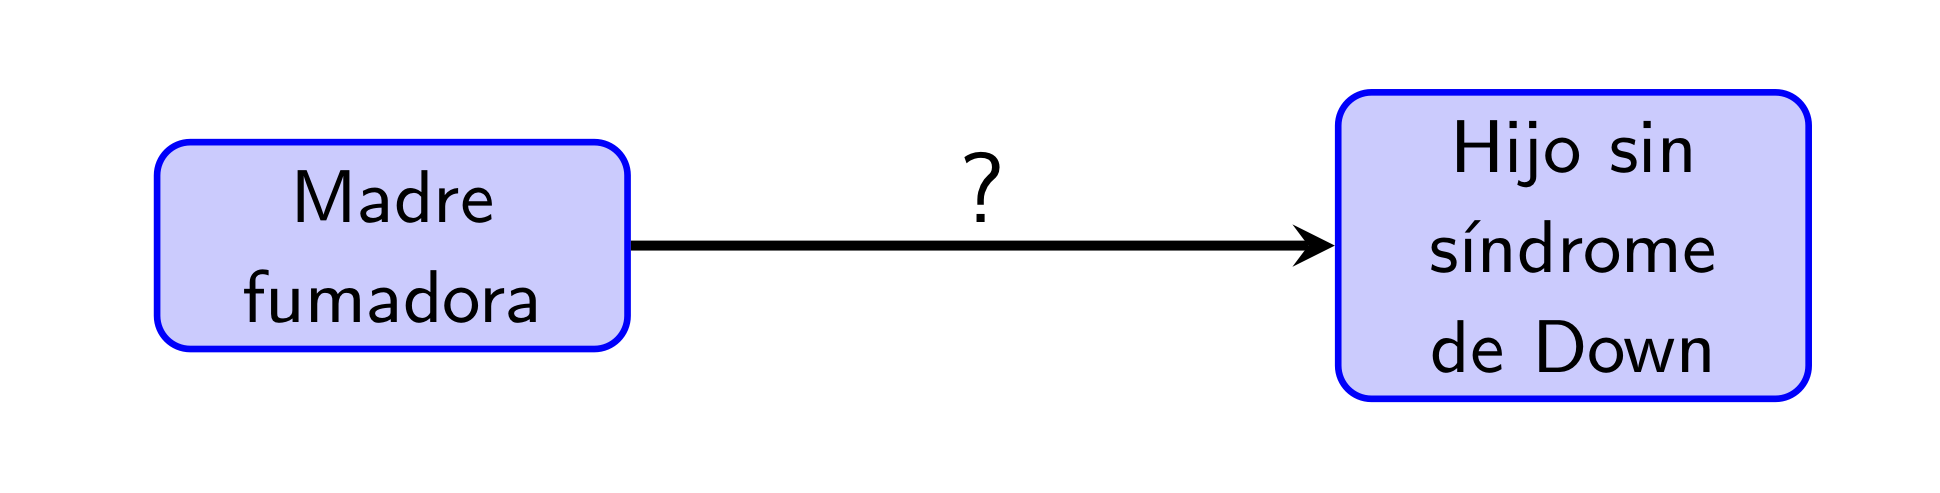
\includegraphics[width=0.8\linewidth]{INREMDN_files/figure-html/Down1} \end{center}

No, ¡qué va! Más tarde, en el artículo \href{https://academic.oup.com/aje/article/149/5/442/135974}{``Maternal smoking and Down syndrome: the confounding effect of maternal age''} (C. L Chen \emph{et al}, \emph{American Journal of Epidemiology} 149 (1999), pp.~442-446) se observó que no se había tenido en cuenta la edad de las madres. Las madres jóvenes suelen ser fumadoras con mayor frecuencia que las no tan jóvenes, y las madres de más de 40 años tienen una mayor frecuencia de hijos con síndrome de Down. Aquí la edad es el factor confundidor que hace que parezca que las mujeres fumadoras tienen menor probabilidad de tener hijos con síndrome de Down, cuando en realidad son las madres jóvenes las que son más fumadores y tienen menos hijos con síndrome de Down.

\begin{center}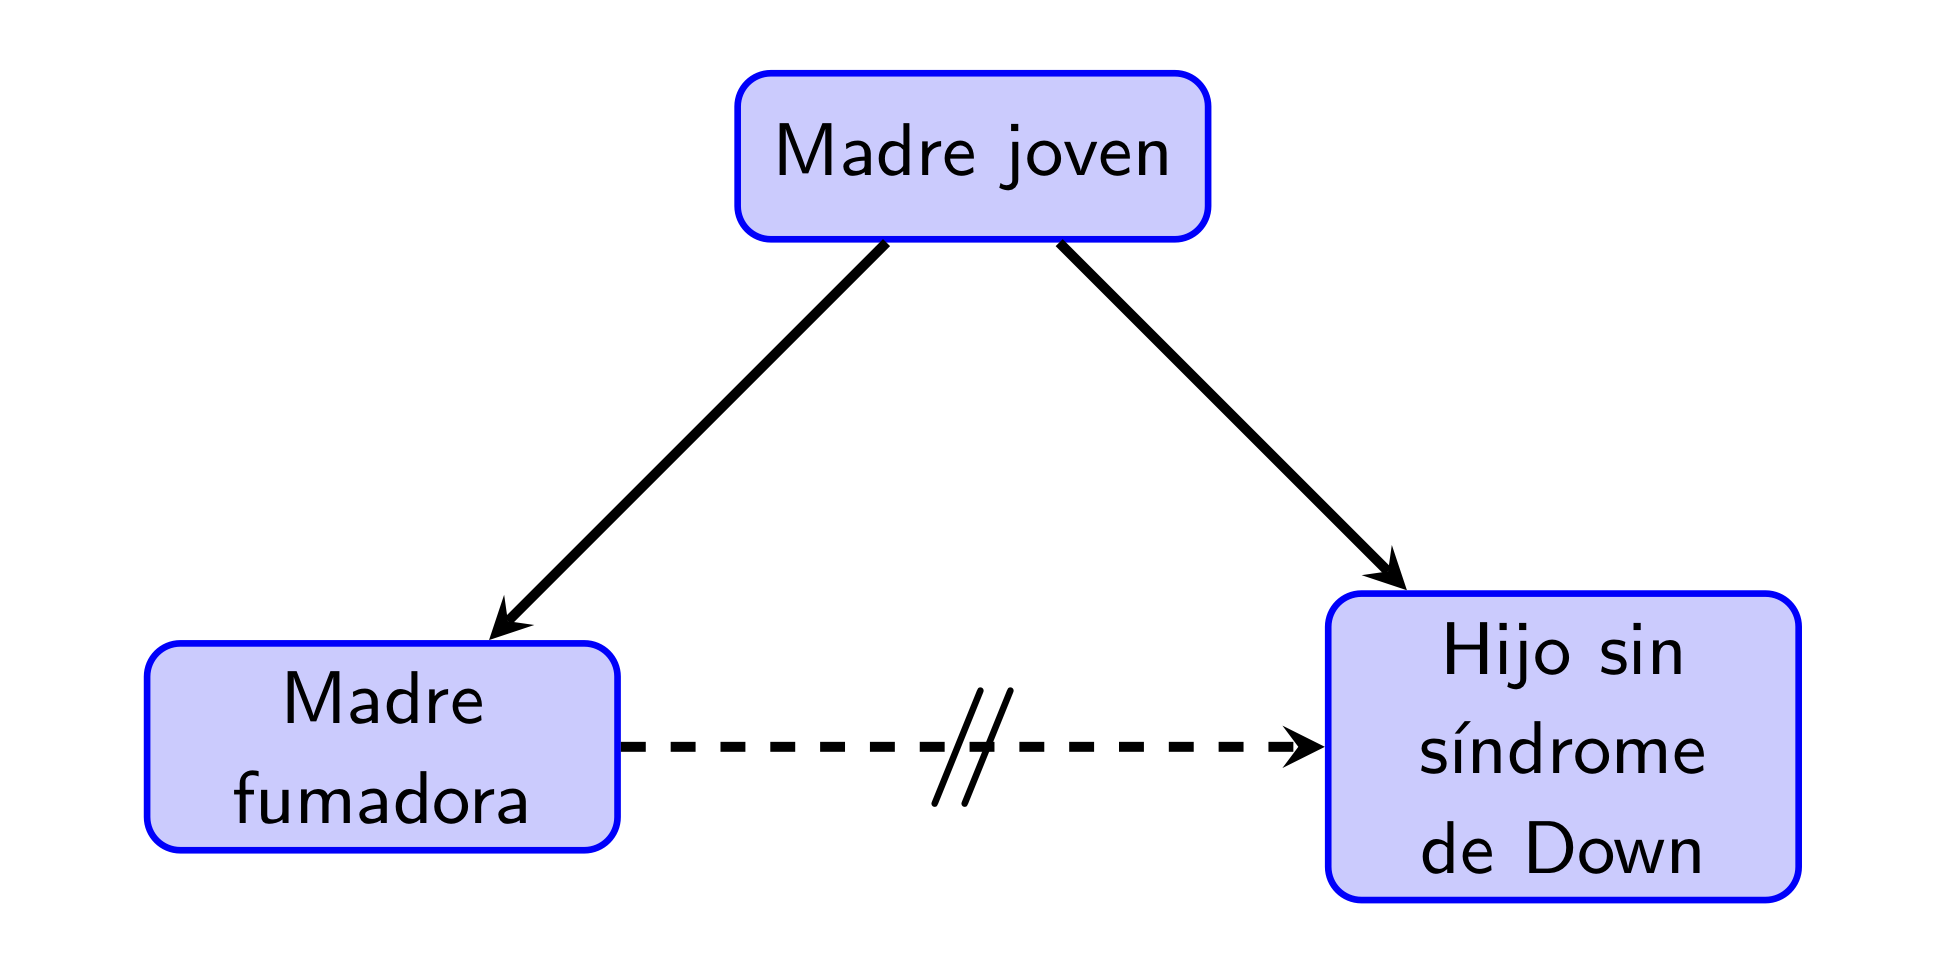
\includegraphics[width=0.8\linewidth]{INREMDN_files/figure-html/Down2} \end{center}

Seguimos con los inconvenientes. \textbf{Los estudios de casos y controles son muy susceptibles a algunos tipos de sesgos concretos} relacionados con la manera cómo se recogen los datos. Un \textbf{sesgo} en un estudio es un error sistemático que afecte a los datos recogidos y pueda perjudicar la corrección de las conclusiones obtenidas. Estudiaremos el tema de los sesgos en general con más detalle en la Sección \ref{sec:sesgos}. Por ahora, vamos a anotar varios sesgos típicos que pueden darse en estudios de casos y controles.

\begin{itemize}
\tightlist
\item
  Si los datos sobre la exposición a riesgos se recogen mediante entrevistas o cuestionarios, los sujetos pueden mentir (recordad la máxima ``Todo el mundo miente'' del Dr.~G. House y los internistas en general), consciente (para ocultar comportamientos de los que se avergüencen, para contentar el entrevistador,\ldots) o inconscientemente (por haber olvidado detalles relevantes). O al menos puede que no recuerden bien los detalles. En ambos casos diremos que se produce un \textbf{sesgo de recuerdo}.
\end{itemize}

\begin{rmdromans}
Hay \href{https://academic.oup.com/jnci/article-abstract/21/4/713/869173}{un estudio famoso} en el que se preguntó a un grupo de hombres si estaban circuncidados: un 34\% de los que contestaron que sí, en realidad no lo estaban, y un 34.6\% de los que contestaron que no, en realidad sí que lo estaban.
\end{rmdromans}

\begin{itemize}
\item
  En particular, se puede dar un \textbf{sesgo de recuerdo diferencial}, ya que los casos y los controles pueden recordar datos relevantes de manera diferente. Si uno tiene un percance, suele recordar con más frecuencia los detalles previos al mismo para buscar ``qué hizo mal'' que una persona que no lo haya tenido.
\item
  También se puede dar un \textbf{sesgo de supervivencia}, si solo se estudian individuos ``vivos''. Por ejemplo, si queremos llevar a cabo un estudio de casos y controles para una enfermedad rara con una tasa de mortalidad a corto plazo muy alta y tomamos como casos enfermos diagnosticados que estén vivos, puede que bastantes de ellos hayan sobrevivido más tiempo de lo normal a la enfermedad y por lo tanto no sean casos representativos.

  Pero si se quiere incluir casos ya fallecidos, seguramente habrá que entrevistar a familiares para conocer detalles de su exposición a factores de riesgo y aumenta el peligro de sesgo de recuerdo. Si uno ya ha difuminado en su memoria los riesgos que corría hace 10 años, mucho menos los recordarán sus familiares.
\end{itemize}

\begin{rmdnote}
En estudios de casos y controles para enfermedades raras con tasa de mortalidad a corto plazo muy alta, lo adecuado es tomar como casos enfermos recién diagnosticados y esperar que sean representativos del conjunto de todos los enfermos.
\end{rmdnote}

Por otro lado, hay que tener mucho cuidado en la \textbf{selección de controles}. En teoría, para poder concluir que hay asociación entre la exposición y la enfermedad, sería necesario que:

\begin{itemize}
\tightlist
\item
  Los controles fueran similares a los casos en todos los aspectos salvo en la exposición.
\item
  Los controles fueran representativos de la población de sanos.
\end{itemize}

En la práctica es muy difícil conseguir ambas condiciones, sobre todo si la población de sanos no está bien definida.

Así por ejemplo, en el estudio sobre alcoholismo y cáncer de pulmón del Ejemplo \ref{exm:CAPUA}, la elección de los controles entre individuos hospitalizados podría haber sesgado este grupo. La ingesta desmesurada de alcohol aumenta el riesgo de patologías que no sean cáncer de pulmón pero que impliquen ingreso hospitalario. Por lo tanto, podría ser que el alcoholismo fuera más frecuente entre personas hospitalizadas que en la población en general. Los autores tuvieron que tener mucho cuidado en este aspecto, eligiendo hospitalizados de algo que \emph{a priori} no tuviera nada que ver con el consumo de alcohol.

O en el ejemplo sobre el fracaso del tratamiento de la tuberculosis del Ejemplo \ref{exm:tuberculosisCC}, hubiera sido un error tomar como controles pacientes tratados con éxito de otras clínicas, que pudieran seguir protocolos de tratamiento diferentes, ya que entonces los controles no serían comparables a los casos.

El siguiente es un ejemplo famoso de la importancia de elegir bien los controles:

\begin{example}
\protect\hypertarget{exm:krunkamp}{}\label{exm:krunkamp}En el artículo \href{https://academic.oup.com/cid/article/62/suppl_1/S83/2566657}{``Association Between Malaria and Invasive Nontyphoidal Salmonella Infection in a Hospital Study: Accounting for Berkson's Bias''} (R. Krumkamp \emph{et al}, \emph{Clinical Infectious Diseases} 62 (2016), pp.~S83--S89), se explica un estudio de casos y controles que en realidad fueron dos. El objetivo era determinar si la malaria es un factor de riesgo para la salmonelosis. Bueno, no, de hecho ese era un objetivo secundario: el principal era estudiar si tomar un grupo de controles no adecuado podía cambiar las conclusiones.
\end{example}

Se tomaron como casos todos los niños ingresados en dos hospitales de Ghana con salmonelosis no-tifóidea invasiva (INTS). Entonces:

\begin{itemize}
\item
  En primer lugar, los controles fueron un grupo de niños sin ninguna enfermedad bacteriana. Se obtuvo que la frecuencia de infecciones previas de malaria entre los \textbf{controles} fue significativamente mayor que entre los casos.
\item
  En segundo lugar, los controles fueron todos los niños hospitalizados en los mismos hospitales con otras enfermedades bacterianas. Se obtuvo que la frecuencia de infecciones previas de malaria entre los \textbf{casos} fue significativamente mayor que entre los controles.
\end{itemize}

Naturalmente, el enfoque correcto es el primero, o mejor aún, tomar como controles un grupo de niños sin INTS, sin distinguir si tenían o no otras enfermedades bacterianas. Los autores concluyen que:

\begin{quote}
``El estudio muestra cómo un sesgo de selección puede revertir los resultados si se utiliza un grupo de control inadecuado y añade evidencia sobre la asociación entre la malaria y la INTS.''
\end{quote}

\begin{rmdimportant}
En todo caso, es conveniente siempre preguntarse si la exposición observada en los controles es la esperada en la población sana, o si por el contrario hay algún motivo por el que no tenga por qué serlo.
\end{rmdimportant}

Hemos dejado para el final un inconveniente muy específico de los estudios de casos y controles en el que igual ya habéis caído.

Fijaos en que el objetivo de un estudio de casos y controles es determinar si la exposición a un factor de riesgo aumenta la probabilidad de padecer una enfermedad y estimar en cuánto la aumenta. Por tanto, lo que se querría comparar son las proporciones de enfermos entre los expuestos y entre los no expuestos, para ver si la primera es mayor que la segunda y cuánto mayor es. Pero las proporciones que se observan son justamente las contrarias de las que nos interesan. En un estudio de casos y controles, medimos \textbf{las proporciones de expuestos y no expuestos entre enfermos y sanos}:

\begin{itemize}
\item
  En el estudio sobre consumo de alcohol y cáncer de pulmón, en realidad se observó que entre los enfermos de cáncer de pulmón hubo una mayor frecuencia de consumo de 30 gramos diarios o más de alcohol y 36 paquetes de tabaco anuales o más. Pero lo que queremos saber es si se da más frecuentemente el cáncer de pulmón entre las personas con estos malos hábitos que en el resto de la población.
\item
  En la parte de casos y controles del estudio chino sobre cirujanos ortopédicos y COVID-19, se observó que la proporción de sujetos que no recibieron formación específica reciente sobre control de infecciones fue superior entre los enfermos de COVID-19 que entre los sanos. Pero lo que queremos saber es si la proporción de infectados entre los que no reciben esta formación es superior a la de infectados entre los que sí la reciben.
\end{itemize}

\begin{center}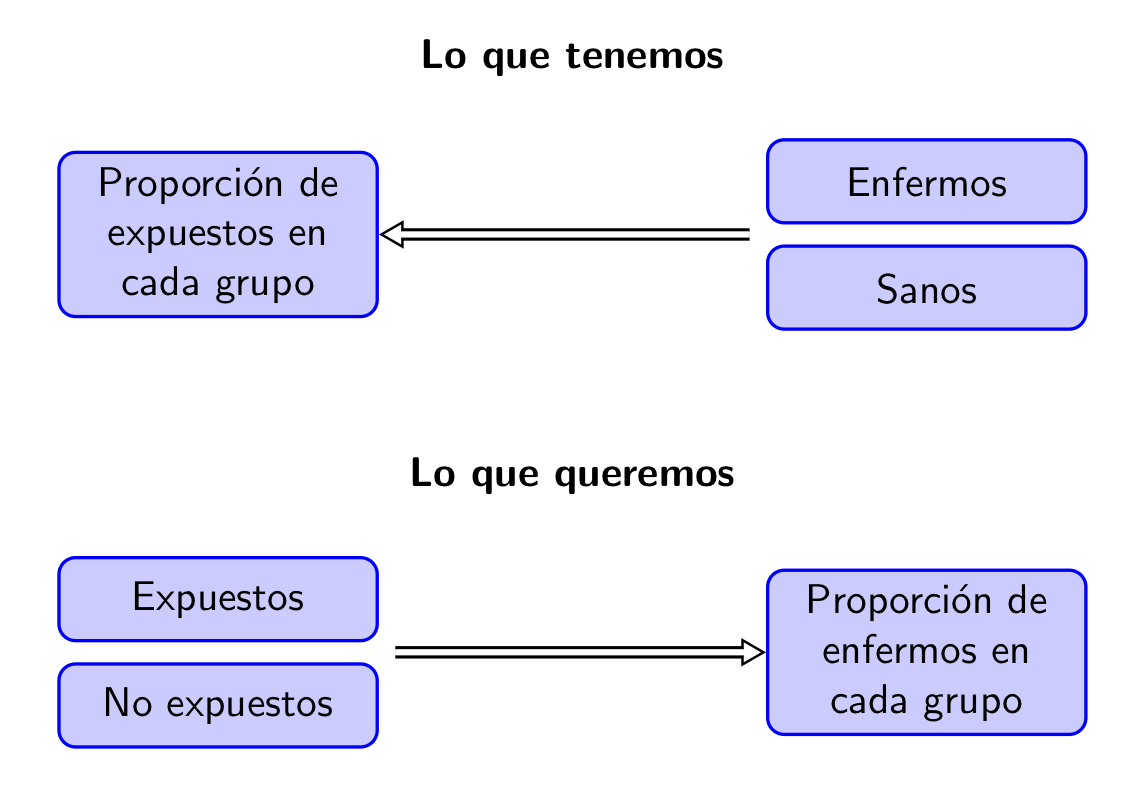
\includegraphics[width=0.8\linewidth]{INREMDN_files/figure-html/queremos} \end{center}

Pues bien, por un lado estamos de suerte: la conclusión global es correcta.

\begin{theorem}
\protect\hypertarget{thm:buensentido}{}\label{thm:buensentido}Si la proporción de expuestos entre los casos es mayor que entre los controles, la proporción de casos entre los expuestos es mayor que entre los no expuestos.
\end{theorem}

Hagamos los cálculos. Supongamos que en nuestra muestra hay \(N\) casos y \(M\) controles. De los \(N\) casos, \(n_1\) estuvieron expuestos al factor de riesgo y \(n_0\) no. Entre los \(M\) controles, sean estos números \(m_1\) y \(m_0\), respectivamente. Llamemos \(E_1=n_1+m_1\) al total de expuestos en la muestra y \(E_0=n_0+m_0\) al de no expuestos. Estos números se resumen en la tabla siguiente:
\[
\begin{array}{r|c|c|c}
& \text{Casos} & \text{Controles} & \text{Total} \\ \hline
\text{Expuestos} & n_1 & m_1 & E_1\\ \hline
\text{No expuestos} & n_0 & m_0 & E_0\\ \hline
\text{Total} & N & M & N+M
\end{array}
\]

Ahora, en términos de estos valores:

\begin{itemize}
\item
  Que haya una mayor proporción de expuestos entre los casos que entre los controles significa que
  \[
  \begin{array}{rl}
  \displaystyle \frac{n_1}{N}>\frac{m_1}{M} & \Longleftrightarrow \displaystyle
  \frac{n_1}{n_1+n_0}>\frac{m_1}{m_1+m_0}\\
  & \Longleftrightarrow n_1(m_1+m_0)>m_1(n_1+n_0)
  \\
  & \Longleftrightarrow n_1m_0>m_1n_0
  \end{array}
  \]
\item
  Que haya una mayor proporción de casos entre los expuestos que entre los no expuestos significa que
  \[
  \begin{array}{rl}
  \displaystyle \frac{n_1}{E_1}>\frac{n_0}{E_0} & \Longleftrightarrow \displaystyle
  \frac{n_1}{n_1+m_1}>\frac{n_0}{n_0+m_0}\\
  & \Longleftrightarrow n_1(n_0+m_0)>n_0(n_1+m_1)
  \\
  & \Longleftrightarrow n_1m_0>n_0m_1
  \end{array}
  \]
\end{itemize}

Como podemos ver, ambas condiciones son equivalentes.

Pero aquí se acaba nuestra suerte.

\begin{rmdcaution}
En un estudio de casos y controles, saber cuántas veces es mayor la fracción de expuestos entre los casos que entre los controles, no nos permite saber \textbf{en general} cuántas veces es mayor la fracción de enfermos entre los expuestos que entre los no expuestos.
\end{rmdcaution}

\begin{example}
\protect\hypertarget{exm:fumadorescancer1}{}\label{exm:fumadorescancer1}Supongamos que tomamos un grupo de 100 enfermos de cáncer de pulmón (casos) y un grupo de 100 no enfermos de cáncer de pulmón (controles), y que entre los casos hay el triple de fumadores que entre los controles.
\end{example}

Supongamos en primer lugar que entre los casos hay 30 fumadores y entre los controles 10. La tabla de frecuencias es
\[
\begin{array}{r|c|c|c}
& \text{Casos} & \text{Controles} & \text{Total} \\ \hline
\text{Fumadores} & 30 & 10 & 40\\ \hline
\text{No fumadores} & 70 & 90 & 160\\ \hline
\text{Total} & 100 & 100 & 200
\end{array}
\]
Entonces, la proporción de enfermos entre los fumadores es de 3/4, es decir, el 75\%, y entre los no fumadores es de 7/16, es decir, el 43.80\%: la primera es 1.71 veces la segunda.

Supongamos ahora que entre los casos hay 90 fumadores y entre los controles 30; observad que sigue habiendo el triple de fumadores entre los casos que entre los controles.

La tabla de frecuencias ahora es
\[
\begin{array}{r|c|c|c}
& \text{Casos} & \text{Controles} & \text{Total} \\ \hline
\text{Fumadores} & 90 & 30 & 120\\ \hline
\text{No fumadores} & 10 & 70 & 80\\ \hline
\text{Total} & 100 & 100 & 200
\end{array}
\]

La proporción de enfermos entre los fumadores sigue siendo del 75\% (3 fumadores por cada no fumador), pero ahora entre los no fumadores es de 1/8, es decir, el 12.5\%: la primera es 6 veces la segunda.

En ambos casos había el triple de fumadores entre los casos que entre los controles, pero al invertir las proporciones, han dado cocientes diferentes de las proporciones de enfermos entre fumadores y no fumadores.

Por suerte, como veremos más adelante (Sección \ref{sec:odds}), una pequeña trampa nos permitirá capear este escollo.

\begin{rmdimportant}
El problema que no nos permitía estimar las fracciones de enfermos entre expuestos y no expuestos en el ejemplo anterior era que tomábamos la muestra de casos y controles \textbf{estratificada}, con números ``artificiales'' de casos y controles. Si hubiéramos tomado la muestra transversal, esperaríamos que fuera representativa de la población y en particular esperaríamos que las proporciones observadas de enfermos entre expuestos y no expuestos fueran representativas de la población y las usuaríamos para estimar estas últimas.
\end{rmdimportant}

\begin{rmdcaution}
Si tomamos una muestra estratificada de casos y controles, con unos números prefijados de casos y de controles que no representen las proporciones de enfermos y sanos en la población,

\begin{itemize}
\tightlist
\item
  ni las proporciones de casos entre los expuestos y no expuestos en nuestra muestra
\item
  ni la proporción de expuestos en nuestra muestra
\end{itemize}

no tienen por qué ser representativas de estas proporciones en el total de la población.
\end{rmdcaution}

\begin{example}
\protect\hypertarget{exm:fumadorescancer2}{}\label{exm:fumadorescancer2}Supongamos de nuevo que tomamos un grupo de 100 enfermos de cáncer de pulmón (casos) y un grupo de 100 no enfermos de cáncer de pulmón (controles). Esta muestra no es representativa de la población, contiene muchos más enfermos de cáncer de pulmón de lo que cabría esperar en una muestra representativa de 200 personas (no es cierto que la mitad de la población tenga cáncer de pulmón, ¿verdad?).
\end{example}

Por lo tanto, es de esperar que las proporciones de casos entre los expuestos y los no expuestos no sean representativas de la población, ya que en la muestra hay más casos de los que ``tocaría''.

Y también es de esperar que la proporción de fumadores en la muestra tampoco sea representativa de la población, porque hay más casos de lo que tocaría, y la proporción de fumadores entre los casos es mayor, por lo que la cantidad de fumadores es seguramente mayor de lo que cabría esperar en una muestra transversal de 200 personas.

\hypertarget{estudios-de-cohorte}{%
\section{Estudios de cohorte}\label{estudios-de-cohorte}}

En un \textbf{estudio de cohorte}:

\begin{itemize}
\item
  Se toma un grupo de individuos expuestos a un factor de riesgo y un grupo de individuos no expuestos a dicho factor de riesgo, o más en general, varios grupos de individuos expuestos a diferentes factores de riesgo.
\item
  Se les realiza un seguimiento durante un período de tiempo para comparar \textbf{prospectivamente} (en el futuro) la aparición de una enfermedad en ambos grupos.
\item
  Se determina si es significativamente más frecuente la aparición de la enfermedad entre los expuestos que entre los no expuestos.
\item
  En caso afirmativo, se infiere que, en la población general, la exposición a dichos factores está asociada a una mayor probabilidad de sufrir la enfermedad.
\item
  Como el objetivo es estudiar la aparición de la enfermedad tras la exposición, los individuos participantes han de estar \textbf{sanos} (es decir, sin la enfermedad de interés) en el momento de iniciar su seguimiento.
\end{itemize}

\begin{rmdnote}
El término ``cohorte'' del nombre refiere al grupo completo de individuos al que se realiza el seguimiento, aunque también a veces se llama ``cohortes'' a los subgrupos de la cohorte global definidos por las diferentes exposiciones a factores de riesgo. Por este motivo, a veces se habla de \textbf{estudio de cohortes}, en plural. A nosotros se nos escapará más de una vez, no nos lo tengáis en cuenta.
\end{rmdnote}

\begin{figure}

{\centering 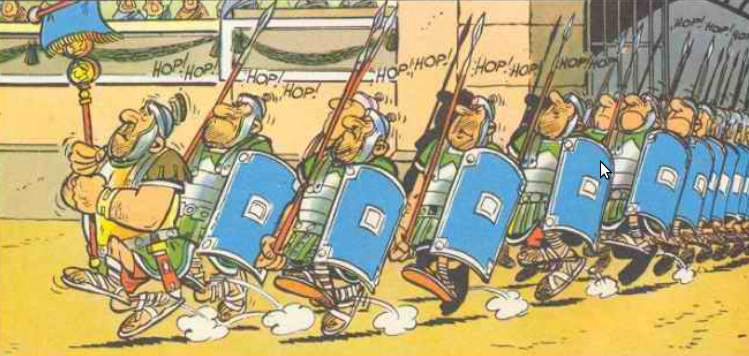
\includegraphics[width=0.8\linewidth]{INREMDN_files/figure-html/cohorteasterix} 

}

\caption{No, esto no es una cohorte en el sentido de esta sección.}\label{fig:cohorteAsterix}
\end{figure}

\begin{rmdcaution}
De nuevo, los términos ``factores de riesgo'' y ``enfermedad'' se han de tomar en un sentido metafórico. Por ejemplo, podríamos comparar grupos de pacientes con una cierta enfermedad bajo diferentes tratamientos para comparar las tasas de curación. En este caso, los ``factores de riesgo'' son los tratamientos, y la ``enfermedad'' la curación.
\end{rmdcaution}

\begin{example}
\protect\hypertarget{exm:EPCOCoh}{}\label{exm:EPCOCoh}Se han llevado a cabo muchos estudios de cohorte para analizar la asociación entre el hábito tabáquico y el desarrollo de enfermedades pulmonares como la EPOC (Enfermedad Pulmonar Obstructiva Crónica). Por ejemplo, el realizado en el marco del \emph{estudio de Rotterdam} (\href{https://link.springer.com/article/10.1007/s10654-016-0132-z}{``Prevalence and incidence of COPD in smokers and non-smokers: the Rotterdam Study''}; N. Terzikhan \emph{et al}, \emph{European Journal of Epidemiology} 31 (2016), pp.~785--792). En este estudio se realizó un seguimiento entre 1989 y 2009 a un grupo (variable, puesto que en algunos momentos se amplió la cohorte, pero vamos a expicar solo la idea general) de unos 14000 sujetos. De ellos, en el momento de incorporarse al estudio un 21.7\% eran fumadores, un 43\% habían sido fumadores pero ya no lo eran, y un 35.3\% nunca habían fumado. En el primer grupo, un 26\% desarrolló EPOC durante el seguimiento; entre el segundo grupo, un 13.6\%, y en el tercero, un 6.4\%. Las diferencias fueron significativas.
\end{example}

\begin{figure}

{\centering 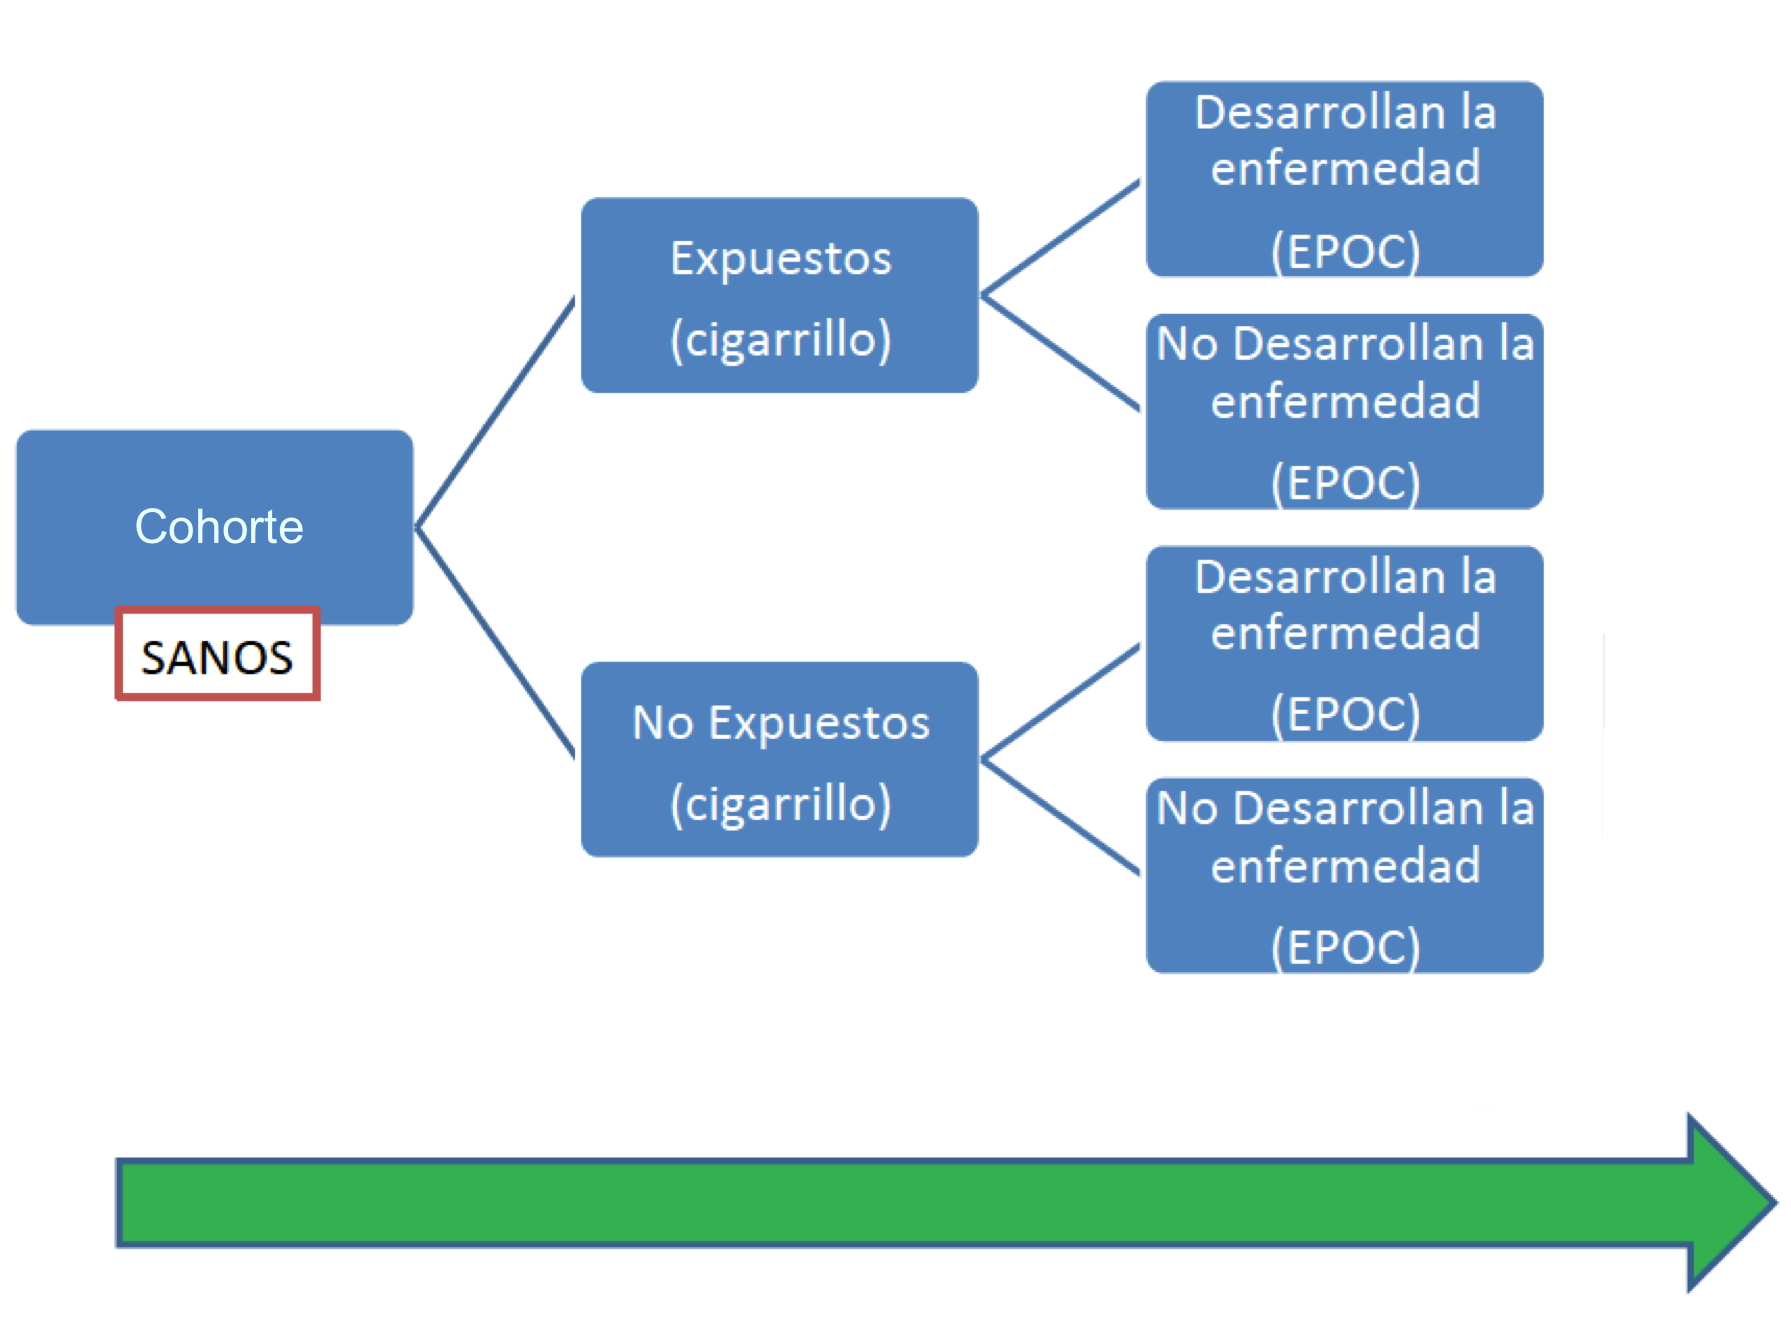
\includegraphics[width=0.8\linewidth]{INREMDN_files/figure-html/epoc} 

}

\caption{Esquema de un estudio de cohorte.}\label{fig:epoc}
\end{figure}

Los estudios de cohorte son también \textbf{observacionales}, \textbf{analíticos} y \textbf{longitudinales}, por exactamente los mismos motivos que los de casos y controles. La información que se analiza va desde el momento en que los sujetos son clasificados según su exposición a factores de riesgo hacia adelante, para ver si desarrollan la enfermedad, y por tanto siempre es prospectiva. Sin embargo, se suele distinguir entre estudios de cohorte \textbf{prospectivos} y \textbf{retrospectivos} según el momento (presente o pasado) en que se realiza la clasificación en expuestos y no expuestos:

\begin{itemize}
\tightlist
\item
  Estudios de cohorte \textbf{prospectivos}: se toman los expuestos y no expuestos a día de hoy, y se estudia su evolución futura (por tanto, esperando a que pase un cierto período de tiempo).
\end{itemize}

El estudio de Rotterdam fue prospectivo. Veamos otro ejemplo de estudio de cohorte prospectivo.

\begin{example}
\protect\hypertarget{exm:IBScohorte}{}\label{exm:IBScohorte}Como su título indica, en el artículo \href{https://www.ncbi.nlm.nih.gov/pmc/articles/PMC27756/}{``Increased risk of irritable bowel syndrome after bacterial gastroenteritis: cohort study''} (L. A. García Rodríguez y A Ruigómez, \emph{British Medical Journal} 318 (1999), 565-566) se publican los resultados de un estudio de cohorte destinado a determinar si tener una gastroenteritis bacteriana aumenta el riesgo de padecer posteriormente síndrome de colon irritable (SCI). Para ello, los autores realizaron un seguimiento a un grupo de pacientes que sufrieron un episodio de gastroenteritis bacteriana y a un grupo de individuos sin gastroenteritis bacteriana. De ambos grupos se excluyeron los pacientes que ya tenían un historial de SCI; recordad que en el inicio del estudio los sujetos han de estar libres de la enfermedad que se quiere ver aparecer. Además también se excluyeron los que tenían algún factor de riesgo conocido del SCI (cáncer de colon, alcoholismo\ldots), para poder ``garantizar'' que su riesgo de aparición del SCI fuera similar, salvo por la gastroenteritis.

Se realizó un seguimiento a ambos grupos durante un año, al cabo del cual un 0.3\% de la cohorte sana y un 4.4\% de la cohorte con gastroenteritis habían sido diagnosticados de SCI.
\end{example}

\begin{itemize}
\tightlist
\item
  Estudios de cohorte \textbf{retrospectivos} o \textbf{históricos}: se toman los expuestos y no expuestos en un cierto momento del pasado, y se estudia su evolución hasta el día de hoy (sin tener que esperar nada de tiempo).
\end{itemize}

\begin{figure}

{\centering 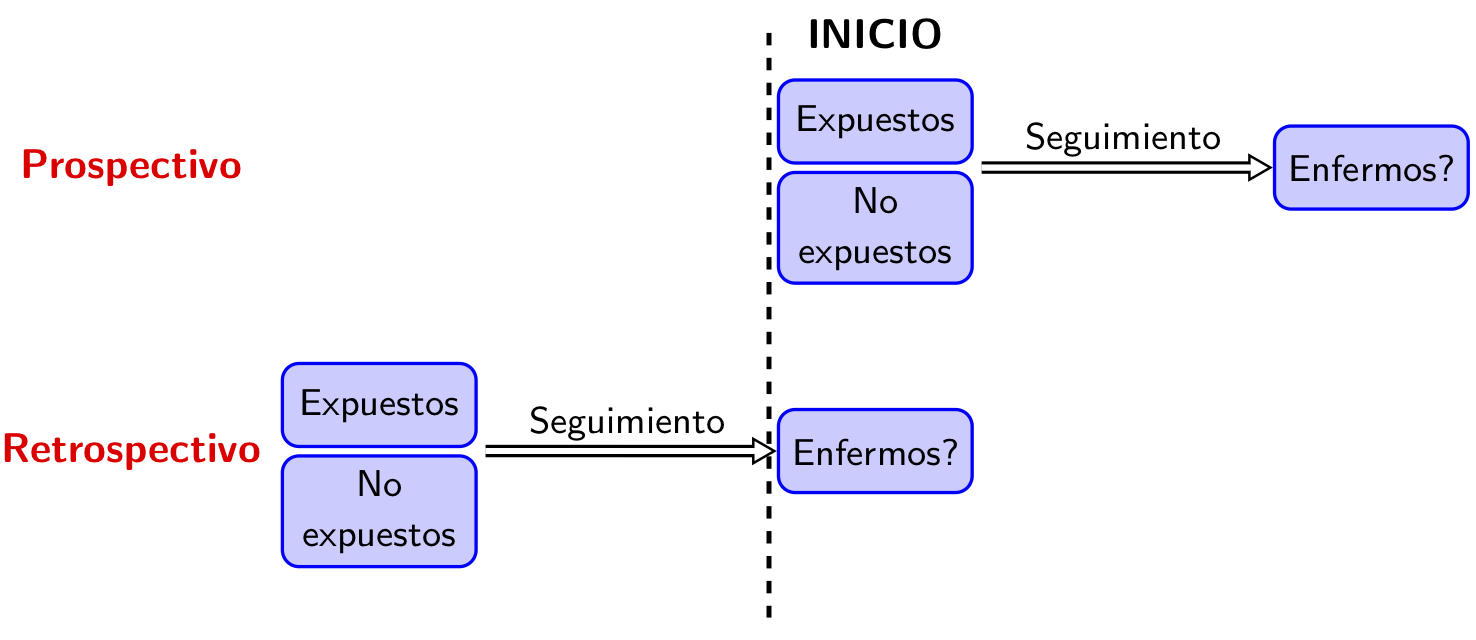
\includegraphics[width=1\linewidth]{INREMDN_files/figure-html/INICIO} 

}

\caption{Estudios de cohorte prospectivos y retrospectivos.}\label{fig:INICIO}
\end{figure}

Veamos un ejemplo de estudio de cohorte retrospectivo.

\begin{example}
\protect\hypertarget{exm:psoriasis}{}\label{exm:psoriasis}En el estudio \href{https://www.sciencedirect.com/science/article/pii/S0025775316306832}{``Mortalidad en pacientes con psoriasis. Análisis de una cohorte retrospectiva''} (W. Masson \emph{et al}, \emph{Medicina Clínica} 148 (2017), pp.~483-488), llevado a cabo en 2016, se tomó una cohorte formada, por un lado, por todos los pacientes del Sistema de Salud de Buenos Aires que a día 1/1/2010 tenían diagnóstico activo de psoriasis, en total 1500, y por otro, por un grupo \emph{de control} formado por 1500 pacientes elegidos al azar entre el resto de sujetos del mismo Sistema de Salud. Se anotaron los sujetos de ambos grupos que fallecieron antes del 30/6/2015. La tasa de mortalidad en el grupo de enfermos de psoriasis fue significativamente más alta que en el grupo de control. La conclusión fue, por lo tanto, que los enfermos de psoriaris tienen un mayor riesgo de defunción a 5 años vista.
\end{example}

Observad las diferencia entre un estudio de casos y controles y un estudio de cohorte. Aunque ambos sean observacionales, analíticos y longitudinales:

\begin{itemize}
\tightlist
\item
  En un estudio de \textbf{casos y controles}, se clasifica el grupo de sujetos en sanos y enfermos y se estudia su exposición \textbf{anterior a esta clasificación} a los factores de riesgo objeto de estudio.
\end{itemize}

\begin{center}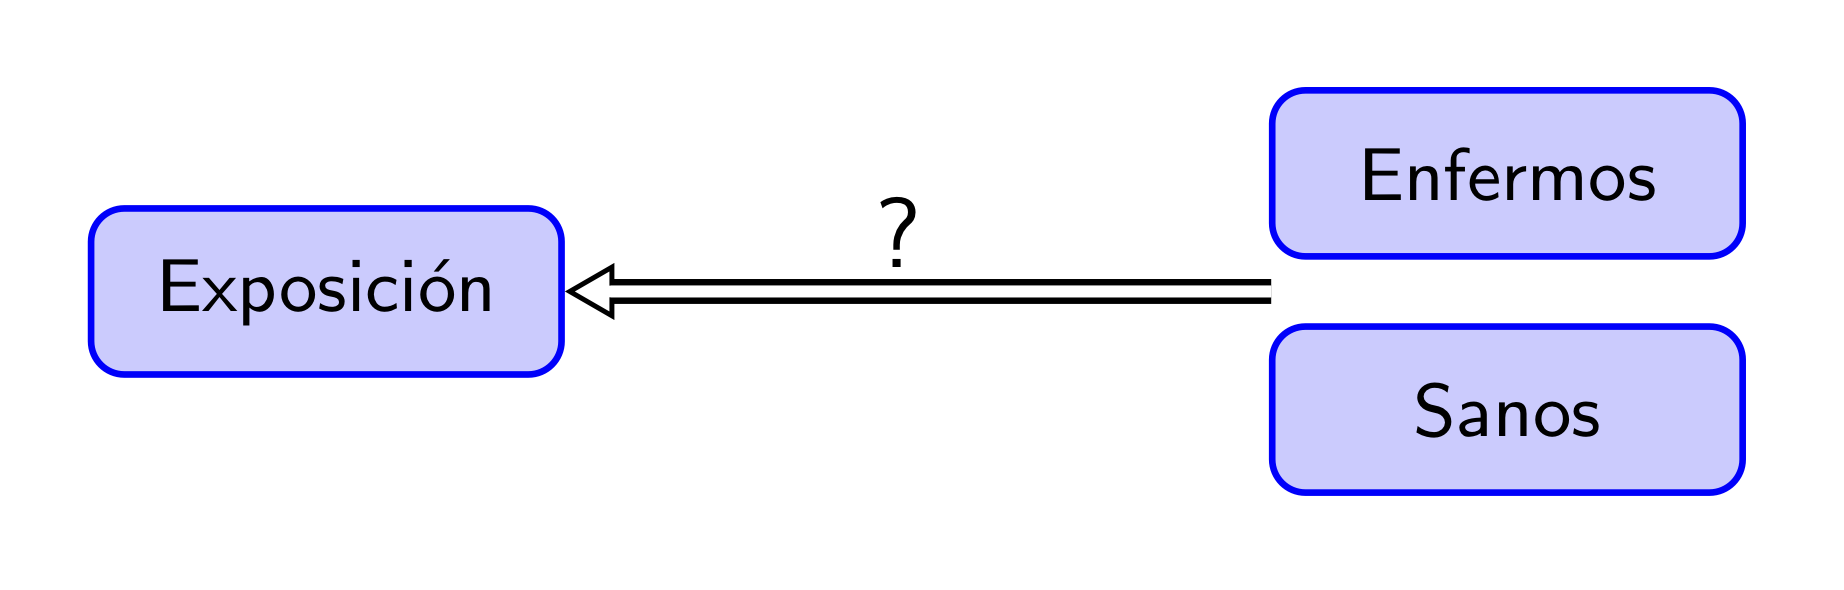
\includegraphics[width=0.8\linewidth]{INREMDN_files/figure-html/CyC} \end{center}

\begin{itemize}
\tightlist
\item
  En un estudio de \textbf{cohorte}, se clasifica el grupo de sujetos \textbf{sanos} en expuestos y no expuestos y se estudia el desarrollo \textbf{posterior a esta clasificación} de la enfermedad objeto de estudio. Si el estudio es de cohorte retrospectivo, la clasificación se realiza en el pasado, pero igualmente se determina si la enfermedad aparece en algún momento posterior a dicha clasificación.
\end{itemize}

\begin{center}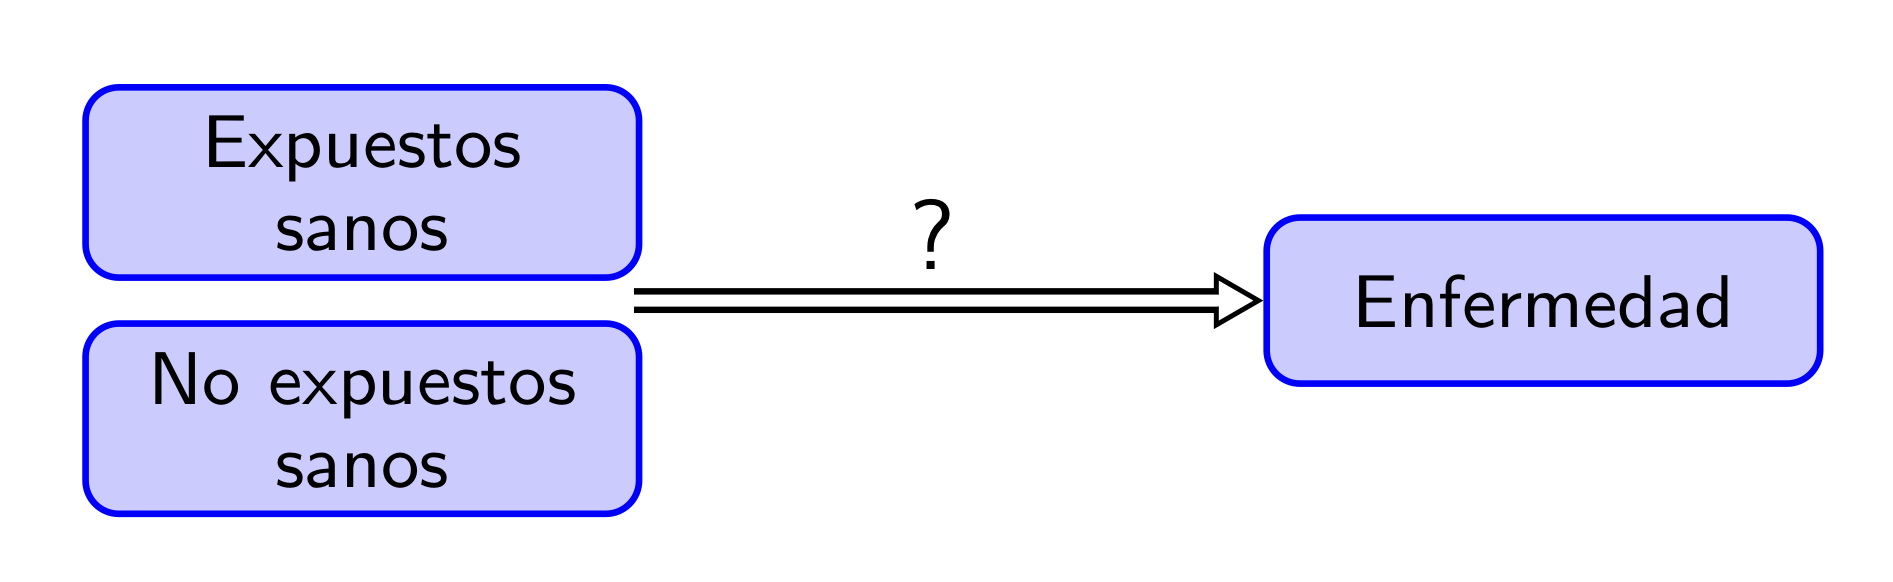
\includegraphics[width=0.8\linewidth]{INREMDN_files/figure-html/Coh} \end{center}

\begin{rmdexercici}
En una \href{http://ns.umich.edu/new/releases/5882}{nota de prensa de la Universidad de Michigan} podemos leer:

\begin{quote}
El peso al nacer tiene efectos importantes y duraderos, según revela un estudio difundido por la Universidad de Michigan. Pesar menos de 2.5 kg al nacer aumenta en un tercio las posibilidades de abandonar la escuela secundaria, reduce las ganancias anuales en alrededor de un 15\% {[}\ldots{]}.
\end{quote}

Considerad la pregunta de investigación siguiente: Las personas con bajo peso al nacer, ¿tienen una mayor probabilidad de fracaso académico?

\begin{itemize}
\item
  Diseñad un estudio de casos y controles cuyo objetivo sea responder a esta pregunta.
\item
  Diseñad un estudio de cohorte prospectivo cuyo objetivo sea responder a esta pregunta.
\item
  Diseñad un estudio de cohorte retrospectivo cuyo objetivo sea responder a esta pregunta.
\item
  ¿Cuál de los tres escogeríais llevar a cabo? ¿Por qué?
\item
  Leed la nota de prensa y decidid qué calificativo describe mejor el estudio realizado por los científicos de la Universidad de Michigan: casos y controles, cohorte prospectivo, cohorte retrospectivo o ninguno de los anteriores.
\end{itemize}
\end{rmdexercici}

Algunas \textbf{ventajas} de los estudios de cohorte:

\begin{itemize}
\item
  Los estudios de cohorte son adecuados para estudiar factores de riesgo raros, por el mismo motivo que los de casos y controles lo son para estudiar enfermedades raras,
\item
  Permiten estimar las probabilidades en el sentido que nos interesa: siempre tiene sentido calcular las proporciones de expuestos y no expuestos que desarrollan una enfermedad, mientras que en un estudio de casos y controles en principio solo tiene sentido calcular las proporciones de enfermos y sanos que previamente estuvieron expuestos al factor de riesgo.
\item
  Los estudios de cohorte retrospectivos suelen ser, como los de casos y controles, relativamente fáciles de llevar a cabo, rápidos y baratos.
\item
  Al hacer un seguimiento desde el momento de la exposición en adelante, son útiles no solo para estimar la proporción de expuestos y no expuestos que desarrollan la enfermedad, sino también la \textbf{incidencia} de la enfermedad en ambos grupos.
\end{itemize}

La \textbf{incidencia} de una enfermedad en una población mide el número de casos \textbf{nuevos} de dicha enfermedad en un período de tiempo. ``Nuevos'' quiere decir que no se cuentan en la incidencia los sujetos que ya estaban enfermos en el momento de iniciar el período de tiempo, pero las recaídas de un mismo individuo sí que cuentan como casos nuevos en la incidencia.

Hay un poco de jaleo con la terminología precisa relacionada con la incidencia, de manera que si consultáis fuentes diferentes encontraréis definiciones ligeramente diferentes. Para fijar el lenguaje, en este curso vamos a distinguir entre \textbf{incidencia acumulada} y \textbf{densidad de incidencia}.

La \textbf{incidencia acumulada}, o simplemente \textbf{incidencia} a secas, es el \textbf{número, o la proporción, de casos nuevos} de la enfermedad durante un período de tiempo concreto.

Por ejemplo, las siguientes frases refieren a la incidencia acumulada:

\begin{itemize}
\item
  ``En los últimos siete días las Islas Baleares han contabilizado 1970 contagios de COVID-19.''
\item
  ``En los últimos 14 días se han detectado en las Islas Baleares 249 casos por cada cien mil habitantes.''
\end{itemize}

\begin{rmderror}
Para ser precisos, al calcular la incidencia acumulada como proporción, el denominador no tendría que ser el total de la población, sino el número de individuos sanos en la población al principio del período de tiempo considerado. Como podéis imaginar, no es lo mismo que en una población de cien mil personas, todas sin COVID, una la coja, que en una población de cien mil personas, de las que 99,999 tienen COVID, la última que queda sana la coja.

Por lo tanto, tendríamos que hablar del número de casos de COVID-19 detectados en los últimos 14 días en las Islas Baleares \textbf{por cada cien mil habitantes sin COVID-19}''.
\end{rmderror}

Naturalmente, si el número de enfermos en la población es relativamente pequeño y solo conocemos una aproximación del número de habitantes en ese momento y además vamos a dar el resultado sin mucha precisión, no hay mucha diferencia entre dividir por el total de habitantes y dividir por el número de habitantes sanos. Pero la manera correcta de calcularla es la primera.

Por ejemplo, a la hora de calcular en septiembre de 2020 que ``en los últimos 14 días se han detectado en las Islas Baleares 249 casos por cada cien mil habitantes'':

\begin{itemize}
\item
  Se conoce la población de las Baleares solo aproximadamente. En realidad, se maneja una estimación de su población a 1 de enero de 2020. Esta estimación era de 1,149,460 habitantes según el \href{https://www.caib.es/ibestat/estadistiques/poblacio/padro/2acef6cf-175a-4826-b71e-8302b13c1262}{padrón de la CAIB}.
\item
  El número de casos activos diagnosticados de COVID-19 (su \textbf{prevalencia}, concepto que trataremos en detalle en la próxima sección) era de algo menos de 2500 enfermos.
\end{itemize}

Está claro que no va a haber mucha diferencia entre dividir el número de casos nuevos por 11.4946 (para obtener el número aproximado de casos nuevos por cien mil habitantes) o por 11.4696 (para obtener el número aproximado de casos nuevos por cien mil habitantes sanos). Sobre todo si no estamos seguros de la exactitud del denominador en ninguno de los dos casos.

Por otro lado, la \textbf{densidad de incidencia} es el \textbf{número medio de casos nuevos} de la enfermedad por unidad de tiempo (durante un cierto período de tiempo).

Por ejemplo:

\begin{itemize}
\tightlist
\item
  ``La densidad de incidencia de la COVID-19 en las Baleares durante la última semana ha sido de 461 contagios diarios.''
\end{itemize}

Por lo tanto,

\begin{itemize}
\item
  La \textbf{incidencia acumulada} mide el número de casos nuevos durante un cierto período de tiempo
\item
  La \textbf{densidad de incidencia} mide la \emph{velocidad media} con la que han aparecido casos nuevos durante un cierto período de tiempo
\end{itemize}

Volviendo a los estudios de cohorte, algunos de sus \textbf{inconvenientes} son:

\begin{itemize}
\item
  Se puede dar el mismo problema con los \textbf{confundidores} que en los estudios de casos y controles.

  Por ejemplo, en el estudio de la mortalidad y la psoriasis del Ejemplo \ref{exm:psoriasis}, se especula con que la causa del aumento de mortalidad sea que ``las modificaciones inmunológicas e inflamatorias observadas en la psoriasis podrían favorecer el desarrollo de la aterosclerosis'', pero no está claro si la causa de las modificaciones inmunológicas e inflamatorias es la psoriasis misma, o si la psoriasis y estas modificaciones se deben a una tercera causa.
\item
  Son poco adecuados para estudiar enfermedades raras, ya que entonces habrá que tomar una cohorte muy grande o realizar el seguimiento durante un período muy largo de tiempo para poder observar una cantidad razonable de enfermos. Por el mismo motivo, los estudios de cohorte prospectivos son poco adecuados para estudiar enfermedades de desarrollo lento.
\item
  Hay que tener en cuenta los \textbf{abandonos}: sujetos de la cohorte inicial a los que se les pierde la pista durante el seguimiento (en los estudios prospectivos) o sobre los que no se tiene información en el momento final del período de tiempo estudiado (en los estudios retrospectivos). Hay técnicas estadísticas específicas para tratarlos.
\end{itemize}

Además, los estudios de cohorte prospectivos tienen los siguientes inconvenientes específicos:

\begin{itemize}
\item
  Puede ser difícil, o al menos costoso, realizar el seguimiento durante un período largo de tiempo de un grupo grande de sujetos
\item
  Se puede dar entre los sujetos seguidos un \textbf{sesgo de conocimiento}, que sucede cuando los individuos modifican su comportamiento habitual al saber que son observados (si los sujetos de la cohorte saben que se les realiza un seguimiento).
\end{itemize}

Los estudios de cohorte retrospectivos resuelven estos inconvenientes, pero presentan uno de propio:

\begin{itemize}
\tightlist
\item
  Se usan datos históricos sobre la exposición, que casi siempre fueron anotados por personas diferentes a las que realizan el estudio y con otros fines (historias clínicas, otros estudios médicos). Esto puede hacer que esos datos no se recogieran de la manera más adecuada para los intereses del estudio presente.
\end{itemize}

\hypertarget{estudios-transversales}{%
\section{Estudios transversales}\label{estudios-transversales}}

En un \textbf{estudio transversal} se toma un grupo de individuos en principio representativo de una población (una \textbf{muestra transversal} de la población) y se miden en un momento concreto varias características de todos ellos: por ejemplo, una enfermedad y los factores de riesgo \emph{presentes en ese momento}. El objetivo es inferir qué asociación hay entre estas condiciones en la población general.

\begin{center}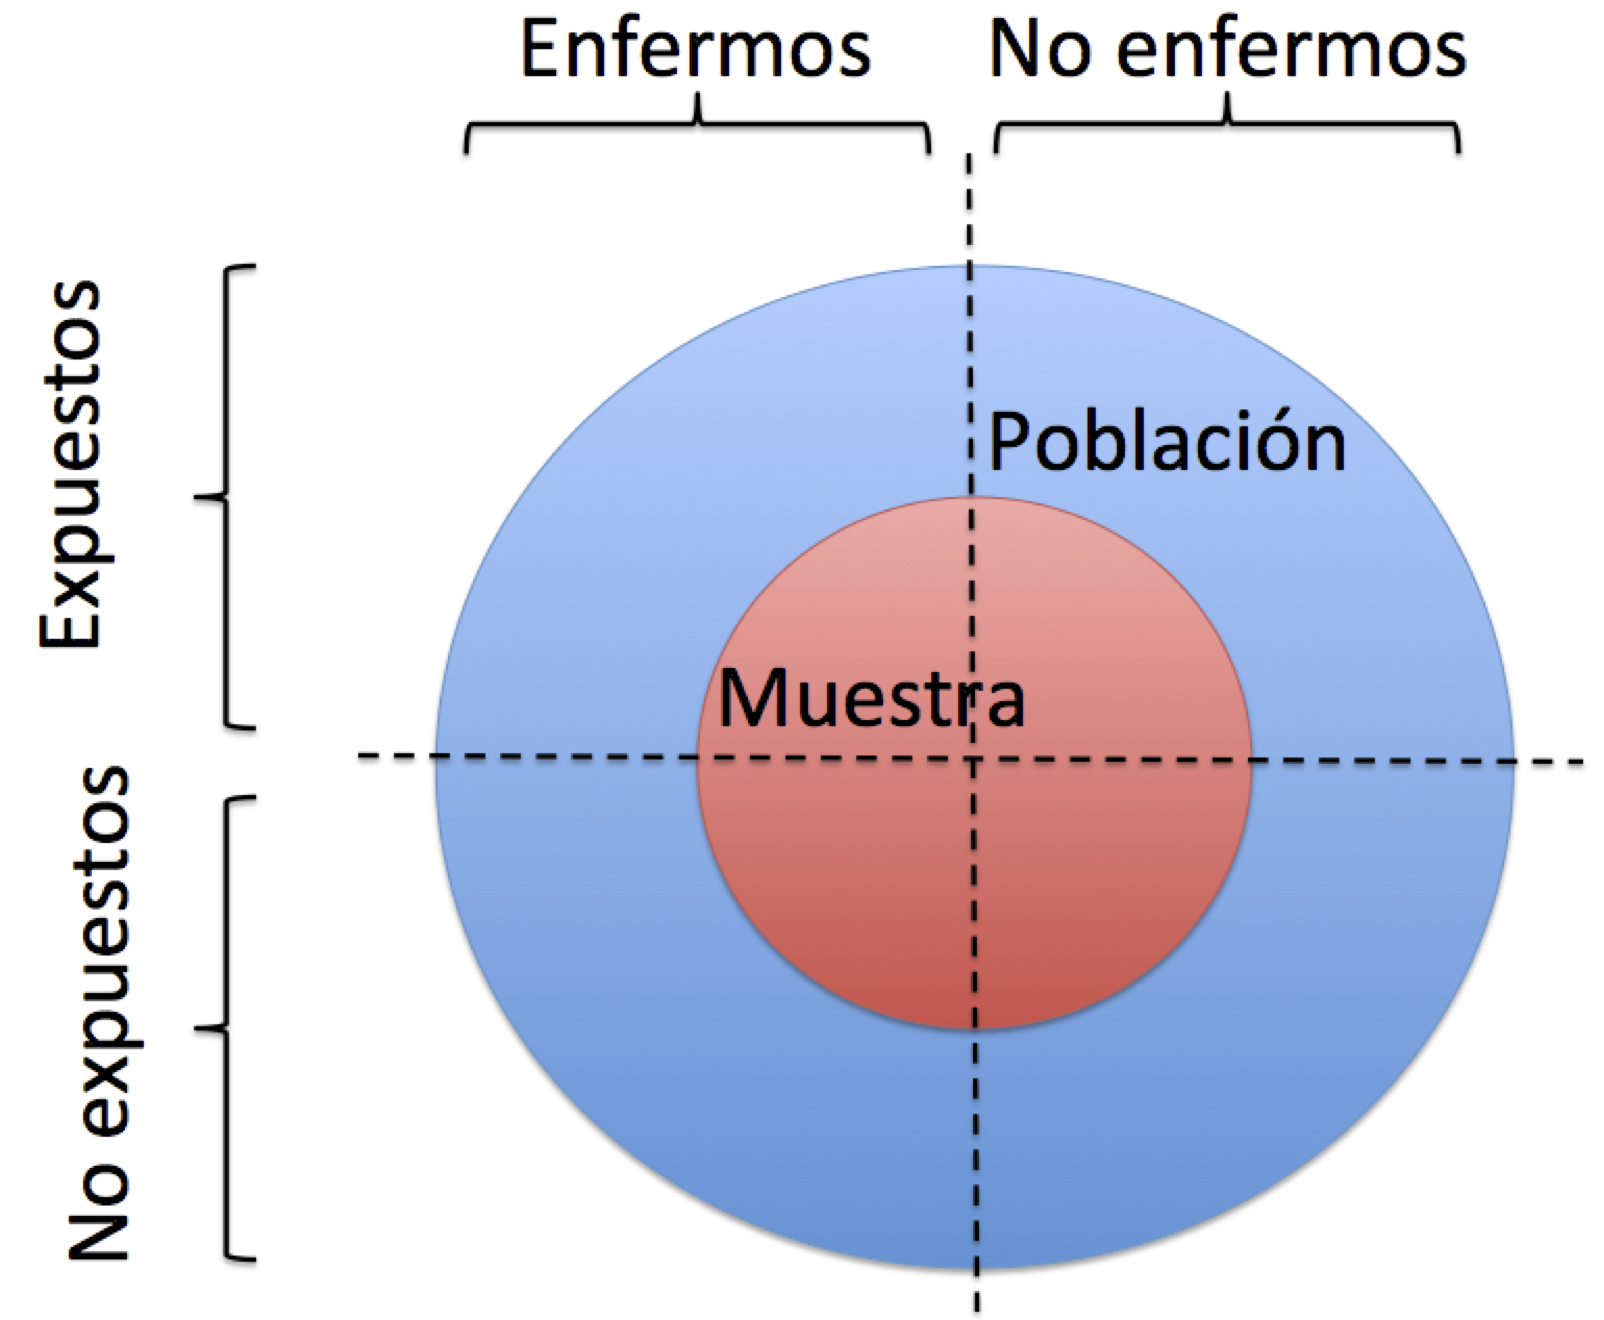
\includegraphics[width=0.6\linewidth]{INREMDN_files/figure-html/transversal} \end{center}

\begin{rmdimportant}
Para que un estudio sea \textbf{transversal} en el sentido de esta sección, es necesario que:

\begin{itemize}
\tightlist
\item
  Sea \textbf{transversal} en el tiempo: la información refiera a un solo momento.
\item
  La muestra sea \textbf{transversal}: sin composición prefijada en clases definidas por las características que se quiere estudiar.
\end{itemize}
\end{rmdimportant}

Una de las utilidades de los estudios transversales es poder estimar la \textbf{prevalencia} de una enfermedad (o de cualquier otra característica): \textbf{la proporción}, o \textbf{el número}, \textbf{de individuos con la enfermedad} en una población en un momento determinado.

\begin{rmdcaution}
No confundáis la prevalencia con la incidencia:

\begin{itemize}
\tightlist
\item
  La \textbf{prevalencia} representa el número \textbf{total} de enfermos en una población en un momento determinado
\item
  La \textbf{incidencia} representa el número de enfermos \textbf{nuevos} en una población en un período de tiempo determinado
\end{itemize}
\end{rmdcaution}

\begin{example}
\protect\hypertarget{exm:unnamed-chunk-40}{}\label{exm:unnamed-chunk-40}En \href{https://www.sciencedirect.com/science/article/pii/S235230181630087X}{``Estimates of global, regional, and national incidence, prevalence, and mortality of HIV, 1980-2015: the Global Burden of Disease Study 2015''} (H. Wang \emph{et al}, \emph{The Lancet. HIV} 3 (2016), e361-87) se afirma que:

\begin{quote}
Desde 2005, la incidencia global del VIH se ha mantenido relativamente constante alrededor de 2.6 millones por año. La prevalencia global del VIH en 2015 era de 38.8 millones.
\end{quote}

Estos 38.8 millones son el total de personas que estuvieron infectadas con VIH en algún momento de 2015, contando los que ya venían infectados de 2014 y los que se infectaron en 2015.
\end{example}

\begin{example}
\protect\hypertarget{exm:corsaib}{}\label{exm:corsaib}En el estudio \href{https://www.revespcardiol.org/es-prevalencia-factores-riesgo-cardiovascular-islas-articulo-13082539}{``Prevalencia de factores de riesgo cardiovascular en las Islas Baleares (estudio CORSAIB)''} (F. Rigo Carratalà \emph{et al}, \emph{Revista Española de Cardiología} 58 (2005), pp.~1411-1419) se tomó una muestra aleatoria de habitantes de las Islas Baleares de la manera siguiente. Se dividió la comunidad en 14 sectores y participaron 3 o 4 médicos de familia por sector (50 en total). A continuación, se seleccionó aleatoriamente a 40 personas entre las adscritas a cada médico participante. A partir de las frecuencias de diversos factores de riesgo cardiovascular en las personas de la muestra, se estimó su prevalencia en el total de nuestra comunidad. Por ejemplo:
\end{example}

\begin{quote}
``Las prevalencias estimadas fueron: tabaquismo del 27\% (el 36.9\% en varones y el 18.7\% en mujeres); hipertensión del 47.8\% (el 52.3\% en varones y el 43.4\% en mujeres); hipercolesterolemia del 24.2\% (el 24.4\% en varones y el 24.1\% en mujeres); diabetes del 11.7\% (el 15.3\% en varones y el 8.4\% en mujeres); obesidad del 27\% (el 24.8\% en varones y el 29\% en mujeres), sobrepeso del 40.1\% (el 48.3\% en varones y el 33.4\% en mujeres) {[}\ldots{]}''
\end{quote}

Este ejemplo es un estudio transversal de prevalencia:

\begin{itemize}
\item
  Se tomó una muestra \textbf{transversal} de la población (la que salió, sin especificar su composición según alguna clasificación de los individuos por factores de riesgo o enfermedades).
\item
  Se midieron algunas características de los sujetos en un solo momento.
\item
  El objetivo era estimar la prevalencia de estas características entre la población de nuestra comunidad.
\end{itemize}

En otros estudios transversales se estima la asociación entre factores de riesgo y enfermedades.

\begin{example}
\protect\hypertarget{exm:quesada}{}\label{exm:quesada}En el estudio \href{https://www.sciencedirect.com/science/article/pii/S0025775316305693}{``Relación entre el mes de nacimiento y la prevalencia de enfermedades crónicas''} (J. A. Quesada y A. Nolasco, \emph{Medicina Clínica} 148 (2017), pp.~489-494), se escogió al azar una muestra de 29,478 españoles adultos y se anotó de cada uno de ellos su sexo y mes de nacimiento y si a 1 de enero de 2017 sufrían, o habían sufrido, alguna enfermedad crónica de una lista de veintisiete. Para ambos sexos se encontraron asociaciones significativas entre el mes de nacimiento y algunas enfermedades crónicas. Por ejemplo, los hombres nacidos en noviembre parecen tener un mayor riesgo de sufrir cataratas.
\end{example}

\begin{rmdromans}
Vamos a ver, en este estudio se tomó una muestra de sujetos y se anotó, por un lado, si tenían o no una serie de enfermedades en un momento determinado y por otro su ``exposición previa a un factor de riesgo'' (su mes de nacimiento). ¿No sería un estudio de casos y controles?

¿Y de cohorte retrospectivo? Porque también podríamos entender que se tomó una muestra de sujetos, se clasificaron según su exposición previa a un factor de riesgo (el mes de nacimiento) y se anotó si desarrollaron posteriormente alguna enfermedad de una lista, ¿no?
\end{rmdromans}

Pues sí, podríamos considerarlo como de casos y controles, aunque anotar no solo si los sujetos tenían las enfermedades a día 1/1/2017, sino también si las habían tenido en el pasado, no encaja del todo con un diseño de casos y controles. Pero como la ``exposición'', es decir, en este caso, el nacimiento, es anterior a cualquier enfermedad que pudieran desarrollar los sujetos, es aceptable.

Y seguramente también podríamos considerarlo de cohorte retrospectivo, aunque, de nuevo, para clasificarlo como tal es necesario que los sujetos no tuvieran las enfermedades en el momento de nacer. Recordad que en los estudios de cohorte, en el momento en el que se clasifican los sujetos según su exposición a factores de riesgo han de estar \textbf{sanos}.

De hecho, los autores dicen que es un estudio transversal, y para nuestro gusto esta sería la clasificación más adecuada, ya que se toma una muestra transversal de la población española y se anotan varias características actuales de los sujetos de la muestra. Pero en cambio el análisis estadístico que realizan sus autores es el típico de un estudio de casos y controles (ya trataremos esta cuestión en la Sección \ref{sec:probaplic2} del tema de Probabilidades). Eso ya es entonces un error.

\begin{rmdimportant}
¿Cuál es entonces la respuesta correcta? La verdad es que cualquiera de las tres. Lo importante no es tanto poner una etiqueta a un estudio como razonar correctamente qué tipo de estudio ``puede ser'' y luego llevar a cabo el análisis estadístico de los datos recogidos de manera consistente con el tipo elegido.
\end{rmdimportant}

\begin{example}
\protect\hypertarget{exm:HS}{}\label{exm:HS}Consideremos el estudio \href{https://www.sciencedirect.com/science/article/pii/S0025775316305759}{``Prevalencia de hipertensión arterial y otros factores de riesgo cardiovascular en la población con hipotiroidismo subclínico''} (L. G. Gil y A. de la Sierra, \emph{Medicina Clínica} 148 (2017), pp.~351-353). En él, se tomó un grupo de 240 pacientes con hipotiroidismo subclínico (HS) visitados en un CAP de Terrassa, y un grupo de 480 pacientes del mismo CAP sin HS (dos por cada uno con HS). Se evaluó en todos estos sujetos la presencia de hipertensión arterial, diabetes etc. El objetivo era comparar la prevalencia de estas patologías entre los pacientes con y sin HS.
\end{example}

Aunque toda la información se recogió simultáneamente y el objetivo es estudiar prevalencias, desde el punto de vista del diseño no se trata de un estudio transversal. Fijaos en que no se tomó una muestra ``transversal'' de sujetos al azar, se analizó si tenían HS o no y se evaluó la presencia de las diferentes condiciones de interés. La muestra que tomaron tenía una composición concreta en términos de una de las características objeto de estudio (HS): dos sujetos sanos por cada enfermo. Esta composición no refleja la de la población (no es cierto que un tercio de la población tenga HS: su prevalencia está entre el 4\% y el 8\%, pudiendo llegar al 16\% entre la población mayor de 60 años). Como lo que interesa es comparar la frecuencia de diversas condiciones entre enfermos de HS y sujetos sin HS, el estudio podría considerarse de cohorte, tomando como expuestos los enfermos de HS. O de casos (los enfermos de HS) y controles (los no enfermos de HS), también sería correcto. Lo importante es analizar los datos consecuentemente

En este caso los autores del estudio lo clasifican como de casos y controles y analizaron los datos de manera correcta según esta clasificación. Como veremos en el tema de Probabilidades, haberlo considerado de cohorte hubiera dado lugar a conclusiones más fáciles de entender, así que nosotros seguramente hubiéramos optado por clasificarlo como de cohorte.

\begin{rmdromans}
¿De cohorte? ¿Y qué pasa con la condición de que los individuos han de estar ``sanos'' en el momento de clasificarlos en expuestos y no expuestos?

Sí, tenéis razón, estamos forzando un poco la definición de estudio de cohorte. Pero la condición de que los individuos de la cohorte han de estar sanos al empezar a correr el tiempo de seguimiento es para poder estudiar \emph{la aparición posterior de la enfermedad}, con el objetivo final de encontrar evidencias de que la exposición causa la enfermedad. En este estudio no les interesaba la aparición posterior de nada, sino lo que pasaba en ese momento. Por ejemplo, qué proporciones de sujetos con y sin HS son hipertensos.
\end{rmdromans}

¿Cómo hubiera sido un estudio transversal? Pues si los investigadores hubieran tomado una muestra al azar de 720 pacientes del CAP y por pura casualidad hubieran salido 240 pacientes con HS y 480 sin HS. Entonces se podría estimar que un tercio de la población de Terrassa asignada a ese CAP sufre de HS y tocaría investigar las causas de esta anomalía.

\begin{rmdcaution}
Es importante observar la diferencia entre un estudio transversal y un estudio descriptivo de tipo serie de casos o \emph{survey}. En ambos casos se toma un grupo de sujetos y se miden una serie de características de los mismos en un momento concreto. Pero:

\begin{itemize}
\item
  \textbf{Los estudios transversales son analíticos}: El objetivo de la descripción de los individuos de la muestra es inferir asociaciones entre características en el total de la población de la que se ha obtenido la muestra.
\item
  \textbf{Las series de casos y los} \emph{surveys} \textbf{son descriptivos}: El objetivo de la descripción de los individuos es exclusivamente ese, describir las características de este grupo de individuos, sin pretender generalizar las observaciones a una población mayor.
\end{itemize}
\end{rmdcaution}

En el ejemplo anterior sobre HS, un estudio descriptivo hubiera consistido en describir (y solo describir) las características de todos los pacientes con HS asignados a ese CAP. Es los que se hizo en el próximo ejemplo, sobre el mismo tema.

\begin{example}
\protect\hypertarget{exm:HSsurvey}{}\label{exm:HSsurvey}En el estudio \href{https://www.sciencedirect.com/science/article/pii/S0212656706703237}{``Hipotiroidismo subclínico en la consulta de atención primaria''} (M. Torné-Coll \emph{et al}, \emph{Atención Primaria} 37 (2006), pp.~175-176) se tomaron todos los pacientes de 11 consultas de un CAP de un pueblo de Barcelona a los que les habían realizado analísis de sangre relacionados con la función tiroidea en algún momento de 2001 y se describieron diversas características de los mismos, con especial atención a cuántos fueron diagnosticados de hipotiroidismo subclínico y sus características. Los autores indican que no se pueden extrapolar los resultados a la población general, porque la muestra estaba formada por individuos a los que se había prescrito un tipo de análisis de sangre concreto, señal de que presentaban síntomas que lo hicieran recomendable.
\end{example}

Se trata de un estudio descriptivo, no un estudio analítico transversal. Por el tamaño de la muestra, 141 individuos, sería un \emph{survey}, pero como la información se obtuvo a partir de las historias clínicas, también se podría considerar una serie de casos. En cualquier caso, descriptivo. Para curarse en salud, los autores dicen que es un ``estudio transversal descriptivo.''

La ventaja principal de los estudios transversales es que, como los de casos y controles y los de cohorte retrospectivos, son relativamente fáciles de llevar a cabo. Además, son el tipo de estudio adecuado para estimar prevalencias.

Los inconvenientes que comparten con los otros estudios observacionales son que puede haber confundidores y que se pueden dar diferentes sesgos en la recogida de datos. Además, al basarse en una muestra ``transversal'' tomada en un momento concreto, es complicado usar un estudio transversal para estudiar enfermedades poco frecuentes o de desarrollo rápido o exposiciones a riesgos poco frecuentes, ya que serían necesarias muestras muy grandes para poder esperar un número suficiente de enfermos o de expuestos. Tampoco permiten estimar incidencias, ya que para ello se necesita contar enfermos en diferentes momentos. Además, son muy susceptibles al sesgo de supervivencia que comentábamos en los estudios de casos y controles, ya que solo muestreamos individuos vivos.

Pero de entre todos sus inconvenientes, el más destacable es que, al usar información sobre un momento concreto, a partir de un estudio transversal en principio \textbf{es imposible obtener ninguna información sobre relaciones temporales} tipo antecedente/desenlace.

Si en una muestra de individuos anotamos, por ejemplo, si en ese momento tienen caries o no y si usan inhaladores para el asma o no, no obtenemos ninguna información sobre si alguna de esas dos condiciones es anterior a la otra y por lo tanto no podemos deducir nada sobre si una podría ser susceptible de ``causar'' la otra.

O por ejemplo, en el estudio del Ejemplo \ref{exm:HS}, se observó que los enfermos de HS tenían un nivel de colesterol significativamente más alto que los controles. Pero la manera como se recogieron los datos no permite saber si el HS precede a la hipercolesterolemia, o si es el colesterol alto el que precede al HS, y por lo tanto no nos podemos ni plantear usarlos para investigar si uno de ellos aumenta el riesgo del otro.

\begin{rmdromans}
Volviendo a la prevalencia, para liar más las cosas los epidemiólogos distinguen entre:

\begin{itemize}
\item
  \textbf{Prevalencia puntual}: lo que nosotros hemos definido como prevalencia, es decir, el número (o la proporción) de personas que tienen la enfermedad en un momento concreto.
\item
  \textbf{Prevalencia de período}: el número (o la proporción) de \textbf{personas} que en algún momento de un período de tiempo concreto han tenido la enfermedad, incluidos los que ya estaban enfermos al inicio del período de tiempo considerado. Si una persona ha tenido varias veces la enfermedad durante el período de tiempo considerado, solo cuenta una vez en este valor.
\item
  \textbf{Prevalencia de vida}: el número (o la proporción) de \textbf{personas} que en algún momento de su vida han tenido la enfermedad. De nuevo, si una persona ha sufrido varias veces la enfermedad a lo largo de su vida, solo cuenta una vez en este valor.
\end{itemize}
\end{rmdromans}

\begin{rmdexercici}
En el examen MIR de 2020 se preguntó lo siguiente: En una población se produjeron 2000 accidentes mortales de tráfico desde el 1 de enero al 31 de diciembre de 2019. ¿Qué medida de frecuencia de accidentes se ha utilizado?:

\begin{enumerate}
\def\labelenumi{\arabic{enumi}.}
\tightlist
\item
  Prevalencia puntual.
\item
  Prevalencia de período.
\item
  Letalidad.
\item
  Incidencia.
\end{enumerate}

Está claro que la respuesta ha de ser (2) o (4); no es prevalencia puntual, porque no es el número de casos en un momento concreto sino durante un período de tiempo, y no es letalidad porque no se trata de la proporción de personas involucradas en accidentes de tráfico que hayan fallecido por esa causa (esa sería la \textbf{tasa de letalidad} de los accidentes de tráfico).

¿Qué responderíais, (2) o (4)? ¿Por qué esa y no la otra?
\end{rmdexercici}

\begin{rmdexercici}
En un \href{https://journals.sagepub.com/doi/abs/10.3181/00379727-26-4143?journalCode=ebma}{estudio llevado a cabo en 1928}, R. Pearl quiso contrastar la hipótesis de que la tuberculosis previene el cáncer. Para ello, de un grupo de 7500 pacientes fallecidos en un hospital concreto, identificó a partir de sus autopsias todos los que tenían cáncer en el momento de fallecer. En total, fueron 816. A continuación, seleccionó al azar otro grupo de 816 de entre los restantes, emparejados con los primeros por edades, raza y sexo. Encontró que un 6.6\% de los enfermos de cáncer y un 16.3\% de los sujetos del otro grupo tenían tuberculosis en el momento de fallecer. Pearl concluyó que la tuberculosis previene el cáncer.

\emph{(a)} ¿De qué tipo de estudio se trata? ¿Cuál es la ``exposición'' y cuál el ``desenlace'' de interés?

\emph{(b)} Teniendo en cuenta que la tuberculosis era una de las causas principales de ingreso en el hospital donde se llevaron a cabo las autopsias, ¿creéis que su conclusión estaba justificada?

\emph{(c)} En caso negativo, ¿se os ocurre alguna manera de usar estas 7500 autopsias para estudiar de manera más concluyente la relación entre cáncer y tuberculosis?
\end{rmdexercici}

\hypertarget{sec:ecol}{%
\section{Estudios ecológicos}\label{sec:ecol}}

En un \textbf{estudio ecológico} se miden las características de interés a nivel de comunidades (países, ciudades, barrios\ldots), no en individuos concretos. Por ejemplo, se comparan las prevalencias de una enfermedad en países con diferentes niveles medios de exposición de sus habitantes a un factor de riesgo.

\begin{example}
\protect\hypertarget{exm:radon}{}\label{exm:radon}En el estudio \href{https://www.sciencedirect.com/science/article/pii/S0025775313009202}{``Radón residencial y cáncer de pulmón. Un estudio ecológico en Galicia''} (R. Barbosa-Lorenzo \emph{et al}, \emph{Medicina Clínica} 144 (2015), pp.~304-348) se consideraron 192 municipios de Galicia en los que se hubieran tomado varias mediciones de radón en domicilios entre 1993 y 2011, y se obtuvieron los números de muertes por cáncer de pulmón en esos municipios durante el período 1980-2009 del Registro de Mortalidad de Galicia. Se observó una asociación positiva entre la mortalidad por cáncer de pulmón y la concentración de radón en domicilios, que fue significativa para los varones pero no para las mujeres. Se concluyó que ``Estos datos evidencian que el radón residencial puede aumentar el riesgo de cáncer de pulmón en varones, aunque en las mujeres no se puede establecer ninguna conclusión''.
\end{example}

¿Es correcta la conclusión? Que se observe una tendencia a que la tasa de mortalidad por cáncer de pulmón entre los varones sea mayor en los \textbf{municipios} con mayor concentración media de radón residencial, ¿aporta evidencia de que el radón residencial aumenta el riesgo de cáncer de pulmón en \textbf{hombres}? (Pista: los autores usan el verbo ``puede aumentar'', no ``aumenta''.)

No.~Este tipo de conclusión es lo que se conoce como \textbf{falacia ecológica}: tomar una asociación positiva entre dos características a nivel de comunidades e inferir una asociación positiva a nivel individual. En general, la asociación a nivel de comunidades no tiene por qué corresponder a una asociación a nivel de individuos. Por ejemplo, este estudio ecológico no aporta ninguna evidencia directa de que los \textbf{hombres} expuestos a una concentración alta de radón en su domicilio tengan mayor probabilidad de cáncer de pulmón. A lo mejor ningún hombre con cáncer de pulmón en los municipios considerados estuvo expuesto a radón residencial. La asociación solo se observó a nivel de municipios.

Veamos otro ejemplo.

\begin{example}
\protect\hypertarget{exm:colombiaBC}{}\label{exm:colombiaBC}En \href{https://onlinelibrary.wiley.com/doi/abs/10.1002/ijc.2910150411}{``Environmental factors and cancer incidence and mortality in different countries, with special reference to dietary practices''} (B. Armstrong y R. Doll, \emph{International Journal of Cancer} 15 (1975), pp.~617-631) se compararon las incidencias y tasas de mortalidad de varios tipos de cáncer con el consumo medio de diferentes tipos de alimentos en 23 países (aquellos para los que pudieron obtener estos datos). Se obtuvo, entre otros, el gráfico de la Figura \ref{fig:cccr}, que muestra que la incidencia de cáncer de colon entre las mujeres de un país tiende a ser mayor cuanto mayor es el consumo diario medio de carne roja en el país.
\end{example}

\begin{figure}

{\centering 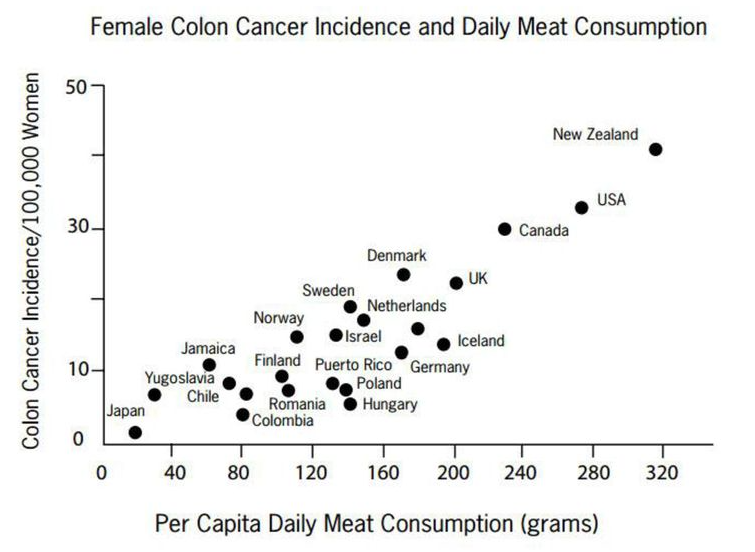
\includegraphics[width=0.6\linewidth]{INREMDN_files/figure-html/meat} 

}

\caption{Incidencia del cáncer de colon entre mujeres en función del consumo diario de carne roja *per capita* en  el estudio sobre factores ambientales y cáncer en diferentes países.}\label{fig:cccr}
\end{figure}

¿Se puede concluir que las mujeres que consumen más carne roja tienen un riesgo mayor de tener cáncer de colon? No, la tendencia observada es a nivel de países, no a nivel individual. Para poder deducir una asociación a nivel de mujeres, sería necesario un estudio en el que se tomara una muestra de mujeres y de cada una se anotara su consumo de carne roja y si desarrolla, o ha desarrollado, cáncer de colon.

¿Para qué sirve entonces un estudio ecológico? Básicamente, para aportar evidencia indirecta de la veracidad de una hipótesis. Esta evidencia indirecta puede reforzar la evidencia obtenida de otras maneras o motivar estudios posteriores. Como además los estudios ecológicos son muy fáciles de llevar a cabo, ya que en general los datos en los que se basan son públicos en bases de datos al alcance de todos y con algo de habilidad se recogen en una tarde, son bastante comunes en epidemiología.

\hypertarget{ensayos-cluxednicos}{%
\section{Ensayos clínicos}\label{ensayos-cluxednicos}}

En todos los tipos de estudios explicados hasta ahora, el investigador se limitaba a \textbf{medir} algunas características de un grupo de personas, sin que su participación en el estudio influyera para nada en dichas características. Es decir, las acciones llevadas a cabo por los investigadores en el paso de recogida de datos eran escoger la muestra y medir sus características, pero, por ejemplo, la exposición a factores de riesgo de los sujetos se debía a razones que no tenían nada que ver con el estudio.

En cambio, en los estudios \textbf{intervencionistas} el investigador \textbf{influye} de manera planificada en las características de los sujetos analizados. Por ejemplo decidiendo quién va a tomar un medicamento y quién no, o quién se va exponer a un riesgo y quién no, y en principio controla todos los aspectos relevantes del proceso (o al menos lo intenta).

En este curso vamos a distinguir entre dos tipos de estudios intervencionistas:

\begin{itemize}
\item
  Estudio \textbf{experimental} (o \textbf{intervencionista aleatorizado y controlado}): En él, los individuos se distribuyen \textbf{al azar} (\emph{aleatorizado}) en \textbf{al menos dos} grupos (\emph{controlado}) que son sometidos a tratamientos \textbf{diferentes} para luego comparar los resultados. Usualmente, uno de los grupos sirve como grupo \textbf{de control}, por ejemplo porque no se les administra ningún tratamiento, o se les administra un \textbf{placebo} (explicamos qué es esto dentro de un rato) o el tratamiento de referencia con el que se quiere comparar un nuevo tratamiento.
\item
  Estudio \textbf{casi-experimental}: Todos los otros estudios intervencionistas.
\end{itemize}

Por ejemplo, el estudio sobre marcha nórdica que usábamos en la Sección \ref{sec:pasos} es casi-experimental, puesto que no hay un grupo de control, solo el grupo a los que se ``administró'' marcha nórdica durante un año.

\begin{rmdcaution}
El adjetivo ``controlado'' en la descripción de los estudios experimentales no significa que el investigador ``controle'' todos los aspectos del estudio: eso ya está (o tendría que estar) incluido en el adjetivo ``intervencionista''. A lo que hace referencia es a la existencia de al menos dos grupos de participantes, uno de los cuales normalmente juega el papel de ``control'' con el que se comparan los resultados de los otros grupos.
\end{rmdcaution}

Como comentaremos más adelante, los estudios intervencionistas suelen aportar una mayor evidencia de la veracidad de sus conclusiones que los estudios observacionales. Pero a menudo es imposible llevarlos a cabo, o al menos no sería ético hacerlo. Por ejemplo, si queremos estudiar si la obesidad aumenta el riesgo de ingreso en UCI en caso de tener COVID-19, ¿cómo podríamos ``intervenir'' para que unos pacientes fueran obesos y otros no? O, retomando el ejemplo del radón y el cáncer de pulmón, no sería de ninguna manera ético exponer a propósito un grupo de personas al radón para ver si desarrollan más cáncer de pulmón que los no expuestos.

\begin{rmdnote}
\textbf{En teoría}, lo estudios experimentales tendrían que permitir establecer una asociación causal entre las variables, porque \textbf{en teoría} el investigador controla completamente las características de los sujetos del estudio, de manera que las diferencias que se den entre los diferentes grupos solo puedan deberse a los diferentes tratamientos. Pero esto es solo \textbf{en teoría}, porque en la práctica es imposible controlarlo todo.
\end{rmdnote}

Se suele llamar \textbf{ensayo clínico} (o simplemente \textbf{ensayo}) a un estudio médico intervencionista con humanos. Un estudio médico en el que se pruebe un tratamiento sobre animales de laboratorio o sobre cultivos de células humanas en placas de Petri no se considera un ensayo clínico (a veces se los llama \textbf{ensayos pre-clínicos}).

En la ejecución de un ensayo clínico, vamos distinguir tres tipos de personas involucradas, o \textbf{partes}:

\begin{itemize}
\tightlist
\item
  Los \textbf{participantes}, es decir, los individuos que forman la muestra que se estudia, a los que se administran (o no) los diferentes tratamientos.
\item
  Las personas encargadas de \textbf{recoger} los datos sobre estos sujetos.
\item
  Las personas encargadas de \textbf{analizar} los datos recogidos, que pueden coincidir o no con las que los recogen.
\end{itemize}

Los ensayos clínicos se clasifican según el nivel de \textbf{enmascaramiento} de sus partes, es decir, según a quién se le oculta información, en:

\begin{itemize}
\item
  \textbf{Abiertos}: Todas las partes del ensayo conocen toda la información sobre qué tratamiento recibe cada sujeto.
\item
  \textbf{Simple ciegos}: Una de las partes del ensayo, normalmente los participantes o el personal encargado de recoger los datos, no conoce el tratamiento que recibe cada sujeto.
\item
  \textbf{Doble ciegos}: Dos partes del ensayo, usualmente los participantes y los encargados de recoger los datos, desconocen el tratamiento que recibe cada sujeto.
\item
  \textbf{Triple ciegos}: Ni los participantes, ni los encargados de recoger los datos, ni los encargados de su análisis estadístico, conocen el tratamiento que recibe cada sujeto.
\end{itemize}

El objetivo del enmascaramiento es \textbf{evitar sesgos en la recogida o el análisis de los datos}. Imaginad por ejemplo que estamos comparando un tratamiento nuevo del dolor articular crónico en el que tenemos muchas esperanzas con simplemente administrar el paracetamol de toda la vida.

\begin{itemize}
\item
  Si el paciente sabe que está tomando el tratamiento nuevo, puede autosugestionarse y sentir menos dolor.
\item
  Si el que entrevista a los pacientes sabe qué está tomando cada uno, puede favorecer los datos sobre el tratamiento nuevo (``De 0 a 10, ¿cómo está hoy de dolor?'' ``Ay, no sé, un 5 o un 6.'' ``¿Ponemos un 5?'').
\item
  Si el que analiza los datos sabe cada individuo de su tabla de datos a qué grupo pertenece, puede escoger de entre todas las técnicas correctas para analizarlos una que favorezca el tratamiento nuevo.
\end{itemize}

\begin{rmdnote}
A menudo se usan los calificativos ``simple ciego'' o ``doble ciego'' en el sentido más general de que se esconde ``algo'' a una o dos partes, pero no tiene por qué ser el tratamiento. Por ejemplo, puede ser que los sujetos sepan perfectamente qué tratamiento reciben, pero que no sepan el objetivo final del estudio para que su conocimiento no influya en su comportamiento.
\end{rmdnote}

Hemos hablado hace un rato de placebo. Un \textbf{placebo} es una substancia similar en todos los aspectos a un tratamiento concreto excepto que es farmacológicamente inactiva. El típico ejemplo son las pastillas de azúcar exactamente con la misma forma y color que las pastillas del tratamiento, pero puede ser algo más exagerado: operar sin hacer nada, solo abrir y cerrar pero siguiendo el ceremonial de las operaciones quirúrgicas, como placebo de la operación quirúrgica ``de verdad'' que se está estudiando.

Usar placebo en un ensayo clínico puede tener varias finalidades:

\begin{itemize}
\item
  \textbf{Enmascarar el ensayo}. Si el grupo de control recibe algo físicamente idéntico al tratamiento pero que no sirve para nada, se puede ocultar a los participantes (y a los que recogen los datos) quién está tomando el tratamiento activo y quién no. En cambio, si a un grupo se les administra un tratamiento y a otro no se les administra nada, es imposible enmascarar el tipo de tratamiento a los participantes.
\item
  \textbf{Evaluar la tasa de curación espontánea}. Al tratar pacientes con algo farmacológicamente inactivo, tenemos un grupo con el que estimar qué proporción de los enfermos se curan sin tratamiento.
\item
  \textbf{Evaluar el \href{https://es.wikipedia.org/wiki/Efecto_placebo}{efecto placebo}}. Se trata de la alteración en la respuesta de un paciente por el mero hecho de recibir tratamiento. Por ejemplo, en un estudio sobre el tratamiento del dolor crónico, puede ser que el paciente note un cierto alivio del dolor simplemente porque ``toma algo'', aunque sea azúcar. Muchas pseudoterapias se basan en este efecto.
\end{itemize}

\begin{example}
\protect\hypertarget{exm:acupuntura}{}\label{exm:acupuntura}Considerad el estudio \href{https://link.springer.com/article/10.1007/s11655-014-1851-1}{``Effect of Zhubin (KI9) acupuncture in reducing alcohol craving in patients with alcohol dependence: a randomized placebo-controlled trial''} (J. S. Lee \emph{et al}, \emph{Chinese Journal of Integrative Medicine} 21 (2015), pp.~307-311). Su objetivo era examinar el efecto de la acupuntura en un determinado punto para reducir el ansia de ingesta de alcohol en alcohólicos. Para ello, se repartió de manera aleatoria 20 pacientes alcohólicos en dos grupos de 10. El grupo de tratamiento recibió acupuntura con agujas reales dos veces por semana durante 4 semanas, y el grupo de control recibió el mismo régimen de acupuntura pero con agujas de placebo (de punta roma, que no perforan la piel). El doctor que practicó la acupuntura conocía qué tipo de aguja usaba, pero los pacientes y el personal encargado de realizarles el seguimiento, no.
\end{example}

Como veis, se trata de un estudio experimental (hay intervención, aleatorización y dos grupos) y es doble ciego. Los resultados del ensayo se resumen en el gráfico siguiente, extraído del artículo:

\begin{center}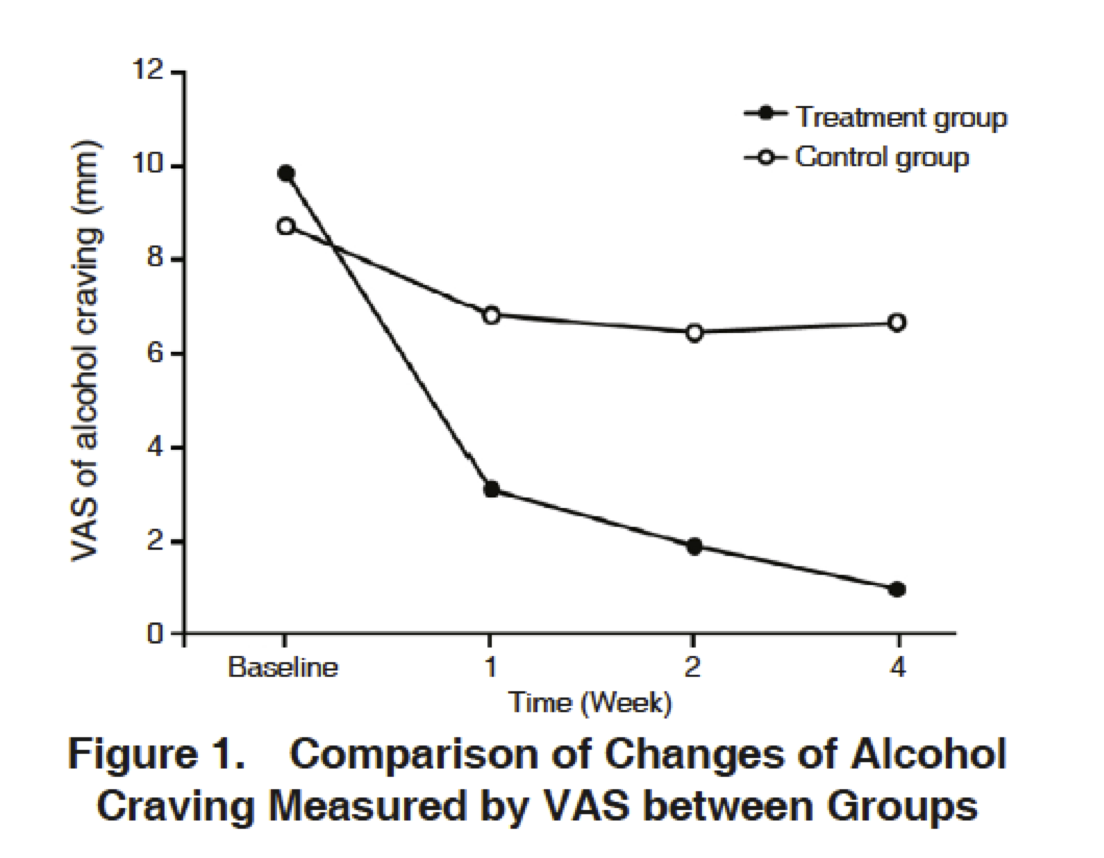
\includegraphics[width=0.6\linewidth]{INREMDN_files/figure-html/acupuntura2} \end{center}

En él, observamos que el ansia por tomar alcohol en el grupo de tratamiento (línea uniendo puntos rellenos) disminuyó mucho más que en el grupo de control, pero que en este último también disminuyó en las primeras sesiones, seguramente debido al efecto placebo.

Otra clasificación importante de los estudios controlados depende de cómo se forman los grupos:

\begin{itemize}
\tightlist
\item
  \textbf{Grupos paralelos}: El grupo de participantes se divide en los diferentes grupos que recibirán los diferentes tratamientos.
\end{itemize}

\begin{figure}

{\centering 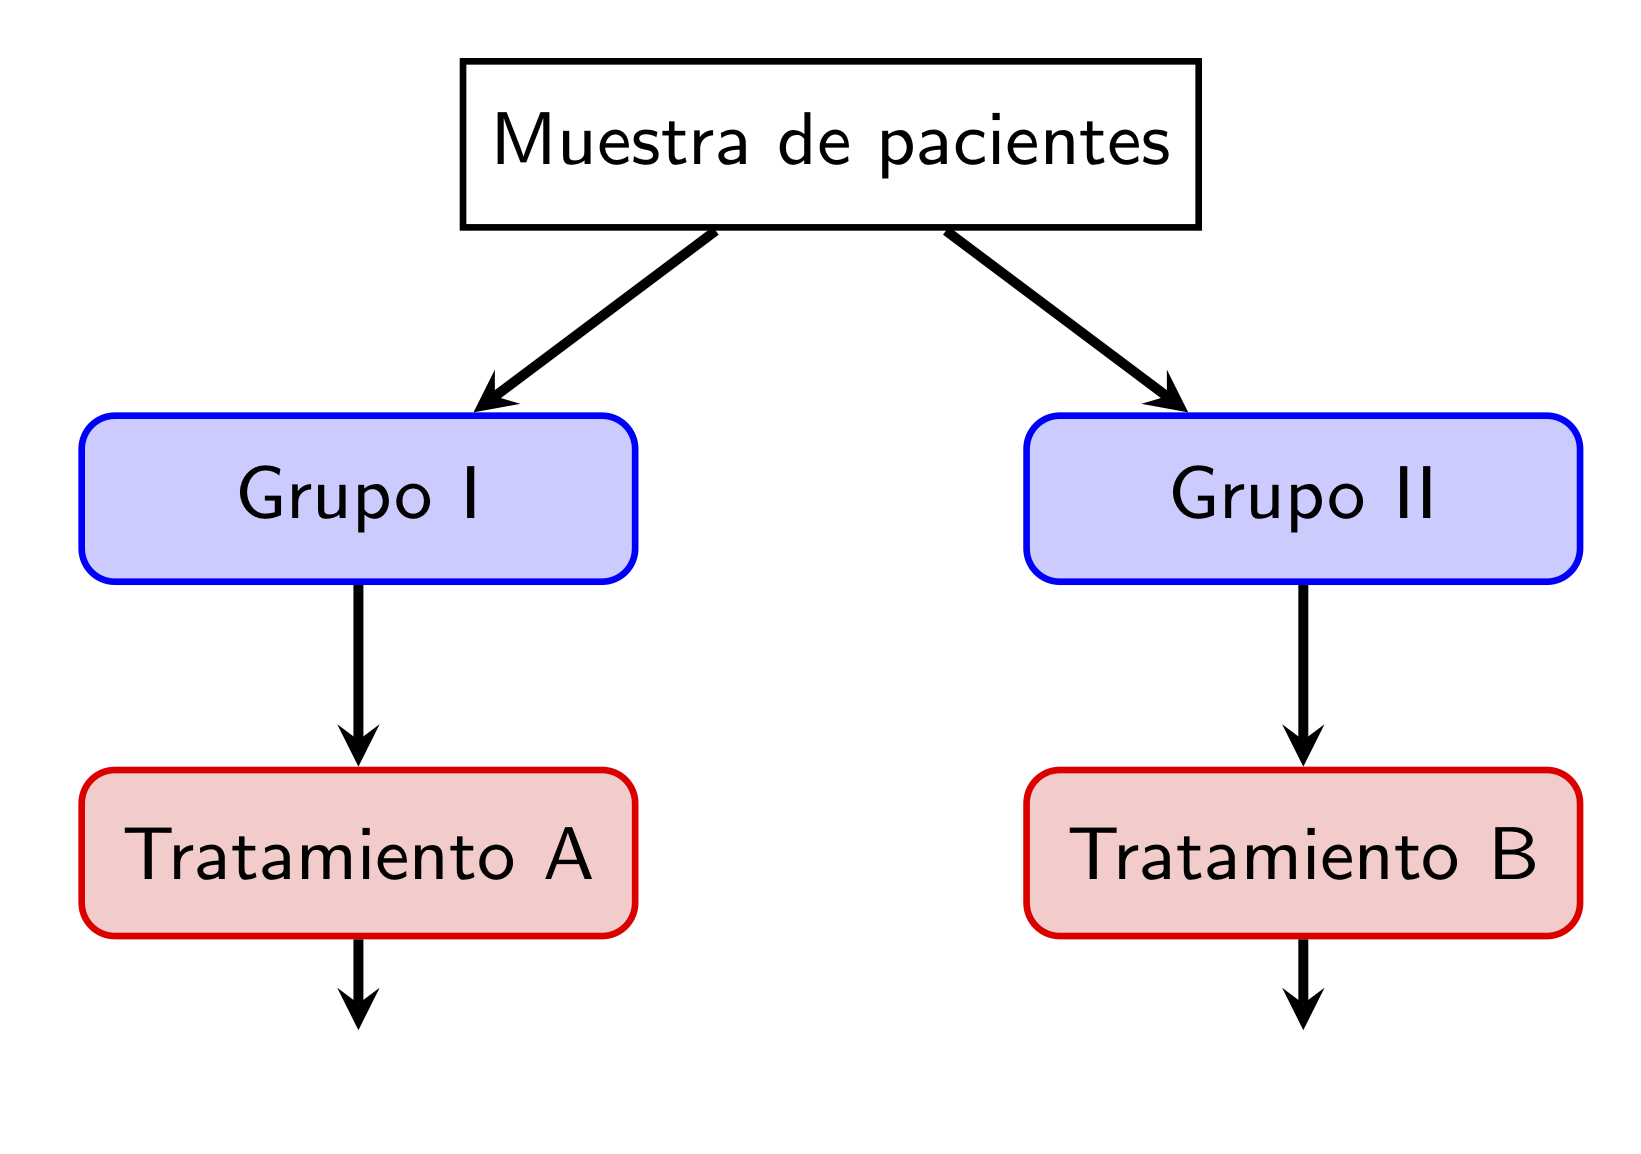
\includegraphics[width=0.5\linewidth]{INREMDN_files/figure-html/EsquemaGP} 

}

\caption{Esquema de un estudio con dos grupos paralelos.}\label{fig:paralelos}
\end{figure}

\begin{itemize}
\tightlist
\item
  \textbf{Grupos cruzados}: Los diferentes tratamientos son administrados a cada sujeto en momentos diferentes, en un orden elegido al azar si queremos que haya aleatorización.
\end{itemize}

\begin{figure}

{\centering 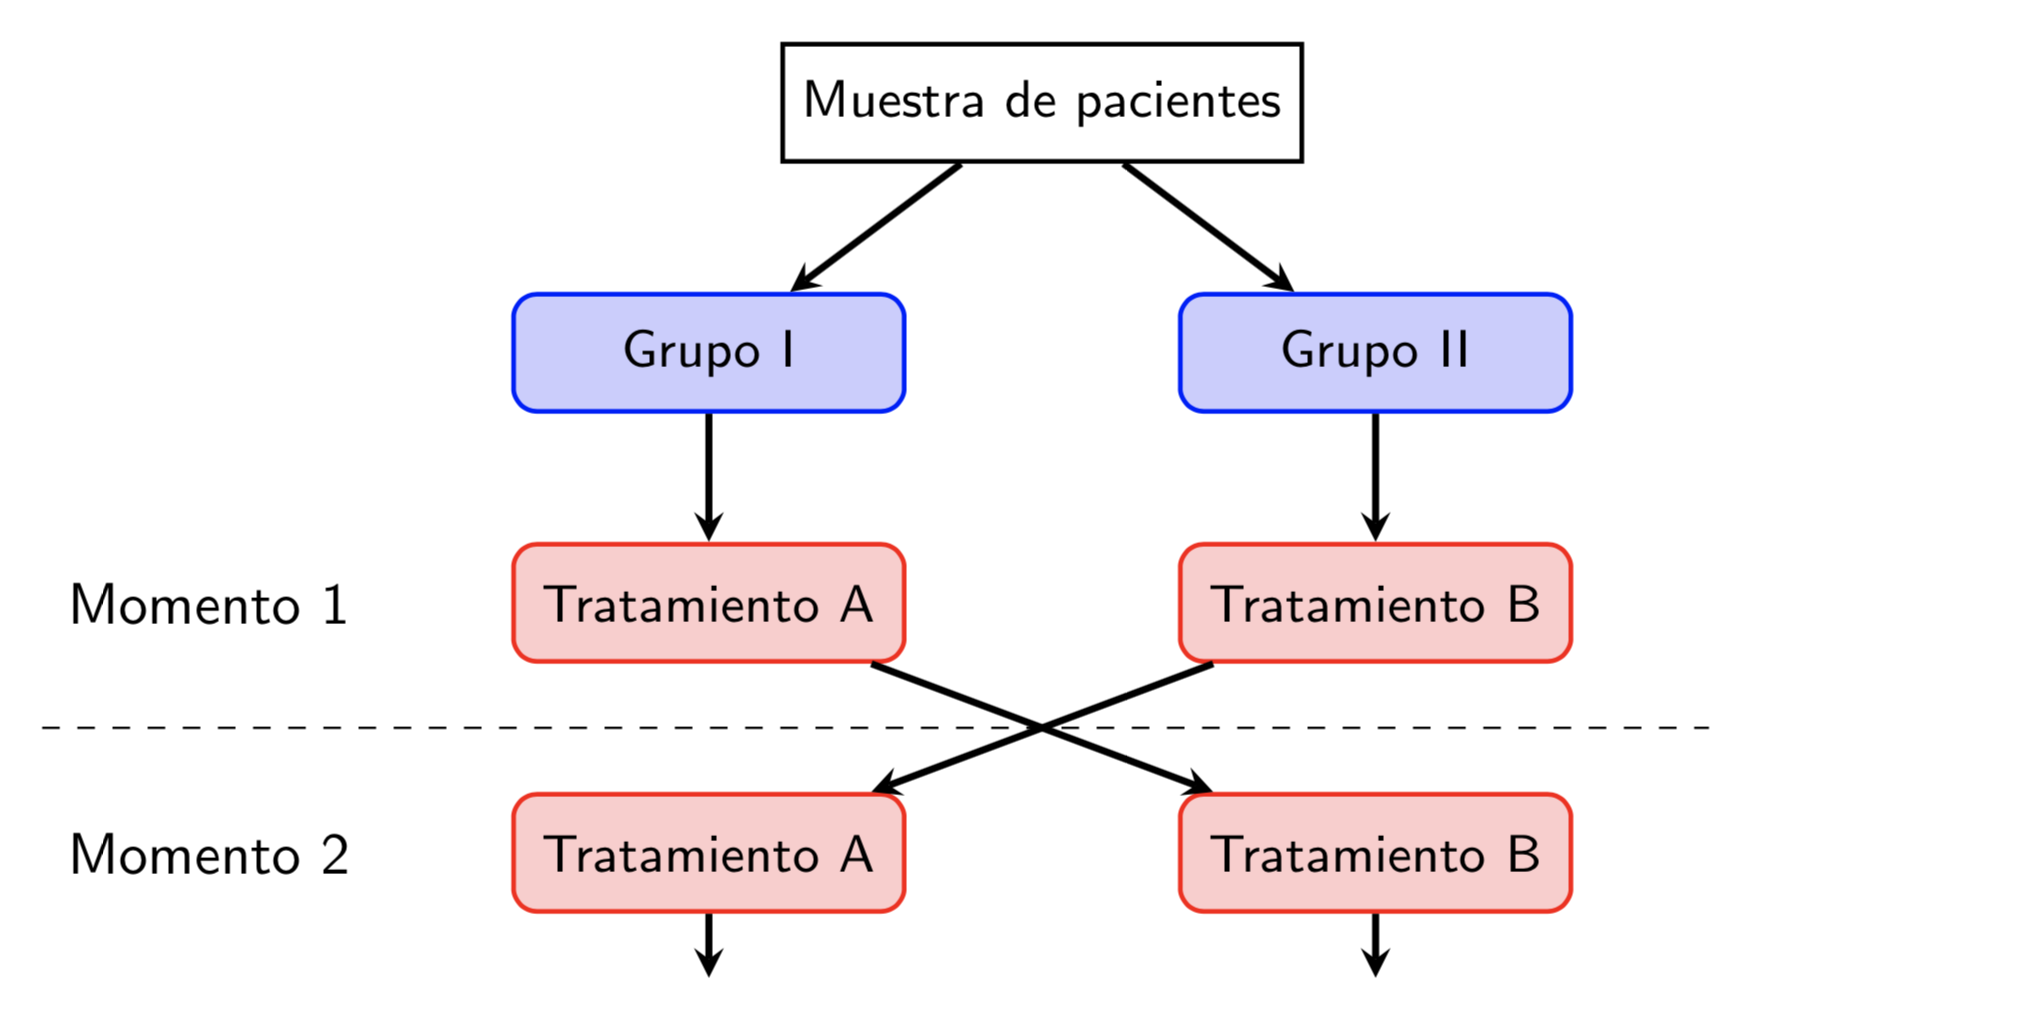
\includegraphics[width=0.8\linewidth]{INREMDN_files/figure-html/EsquemaGC} 

}

\caption{Esquema de un estudio con dos grupos cruzados.}\label{fig:cruzados}
\end{figure}

El estudio de acupuntura mencionado hace un rato fue de grupos paralelos: cada grupo recibió un único tratamiento, diferente en un grupo del otro. Veamos otro ejemplo de estudio con grupos paralelos.

\begin{example}
\protect\hypertarget{exm:baile}{}\label{exm:baile}En el estudio \href{https://www.sciencedirect.com/science/article/pii/S0025775316303116}{``Efectos de un programa de terapia de baile en la calidad de vida, el sueño y la presión arterial en mujeres de mediana edad: un ensayo controlado aleatorizado''} (M. Serrano-Guzmán \emph{et al}, \emph{Medicina Clínica} 147 (2016), pp.~334-339) participaron 67 mujeres de mediana edad prehipertensas e hipertensas. Se asignó cada una al azar a un \textbf{grupo de intervención} (donde siguieron un programa de terapia de baile específico durante 8 semanas, además de su medicación) o a un \textbf{grupo control} (donde continuaron con sus actividades y medicación habitual). 35 mujeres fueron a parar al grupo de intervención y 32 al grupo de control. Se midieron en ambos grupos la presión arterial, la calidad del sueño y la calidad de vida (estas dos últimas mediante indicadores específicos) al principio del estudio y tras las 8 semanas. El grupo de intervención mejoró significativamente sus valores de presión arterial, calidad del sueño y calidad de vida en comparación con el grupo control.
\end{example}

Veamos ahora un ensayo con grupos cruzados.

\begin{example}
\protect\hypertarget{exm:creuat2cec}{}\label{exm:creuat2cec}En el estudio \href{http://www.revistagastroenterologiamexico.org/es-pdf-X0375090612226816}{``Digestión deficiente e intolerancia a lactosa en un grupo de enfermos con colitis ulcerativa crónica inespecífica, Ensayo clínico controlado, cruzado y doblemente a ciegas''} (G. A. Cabrera-Acosta \emph{et al}, \emph{Revista de Gastroenterología de México} 77 (2012), 26-30) participaron 39 pacientes diagnosticados de colitis ulcerativa crónica inespecífica (CUCI). Cada uno de ellos recibió, de forma aleatoria, 12.5 g de lactosa o de maltosa en 250 ml de agua, tras un ayuno de 12 horas. Al cabo de tres días de dieta habitual, cada participante recibió el preparado que no había recibido en la primera prueba. Tras cada sesión, se les realizó un test de intolerancia a la lactosa, siempre el mismo (cantidad de hidrógeno en aire aspirado). Ni los participantes ni el personal que realizó los tests conocía el orden asignado de los productos consumidos. 18 enfermos (un 46\% del total) presentaron digestión deficiente de lactosa.
\end{example}

Observad algunos aspectos de este estudio:

\begin{itemize}
\item
  El ensayo fue \textbf{controlado}, ya que cada sujeto fue el control de si mismo. Se comparó para cada participante su digestión de la lactosa y de la ``no-lactosa'', que es el papel que juega la maltosa en este estudio.
\item
  El ensayo fue \textbf{aleatorizado}, ya que el orden de los productos administrados a cada sujeto fue decidido al azar. De esta manera, se intentó evitar posibles sesgos que podrían haberse dado si todos hubieran consumido cada producto en el mismo día. Por ejemplo, si hubiera algún factor desconocido que influyera en la digestión de la lactosa y que se hubiera dado el día que tocara lactosa a todos.

  Las dos tomas se separaron 72 horas para disminuir el efecto residual del azúcar consumido en la primera prueba.
\item
  La maltosa en agua tiene un aspecto y sabor similar al de la lactosa, por lo que sirvió de \textbf{placebo}.
\item
  El ensayo fue \textbf{doble ciego}: los participantes no sabían qué bebían en cada toma y el personal que realizó los tests de intolerancia a la lactosa y midió sus resultados tampoco sabían qué habían tomado.
\end{itemize}

Es importante recalcar las similitudes y diferencias entre los diseños de cohorte y experimental en estudios para determinar la asociación entre una exposición y un desenlace.

\begin{itemize}
\item
  En ambos estudios se toma un grupo de expuestos y uno de no expuestos.
\item
  En el estudio de cohorte, los sujetos pertenecen a un grupo u otro \textbf{por motivos externos} al estudio: por decisión propia, por criterio clínico, por motivos ambientales, geográficos, genéticos\ldots{} Esto puede hacer que los sujetos con algunas características concretas sean más abundantes en un grupo que en otro.
\item
  En el estudio experimental, los sujetos son asignados por el investigador \textbf{de manera aleatoria} a un grupo u otro. De esta manera se intenta prevenir que los sujetos con algunas características concretas tiendan a aparecer más en un grupo que en otro.
\end{itemize}

\begin{rmdcaution}
Comparad las dos situaciones siguientes.

\begin{itemize}
\item
  En un estudio sobre la eficacia de dos tratamientos, A y B, para una enfermedad, se tomó un grupo de pacientes con esta enfermedad. A cada uno de ellos se le administró A o B según el \textbf{criterio clínico} del médico que los atendió, y se comparó la eficacia de ambos tratamientos.
\item
  En un estudio sobre la eficacia de dos tratamientos, A y B, para una enfermedad, se tomó un grupo de pacientes con esta enfermedad. A cada uno de ellos se les administró A o B \textbf{al azar}, y se comparó la eficacia de ambos tratamientos.
\end{itemize}

El primero sería observacional, más en concreto de cohorte; el segundo, experimental.
\end{rmdcaution}

\begin{rmdexercici}
En un \href{https://www.ncbi.nlm.nih.gov/pmc/articles/PMC2272051/pdf/epidinfect00028-0013.pdf}{famoso estudio}, el \href{https://es.wikipedia.org/wiki/Norman_Gregg}{Dr.~Norman Gregg} estudió 78 casos de recién nacidos con cataratas congénitas de toda Australia, y observó que en 68 de ellos se había diagnosticado que la madre había tenido la rubeola durante la primera parte del embarazo (de los 10 restantes, solo en 2 se descartaba explícitamente que hubieran pasado la rubeola durante el embarazo). Concluyó que había asociación entre la rubeola materna y las cataratas congénitas.

\begin{enumerate}
\def\labelenumi{\alph{enumi}.}
\item
  Por su diseño, ¿de qué tipo de estudio se trata?
\item
  ¿Creéis que la conclusión de Gregg estaba justificada basándose solo en los datos de los 78 neonatos con cataratas? Si sí, ¿por qué? Si no, ¿qué información haría falta para poder llegar a una conclusión?
\item
  Si el estudio de Gregg no fue de casos y controles, diseñad (en detalle: cómo elegiríais los casos y los controles, cómo obtendríais la información etc.) un estudio de este tipo cuyo objetivo sea detectar la posible asociación entre la rubeola materna y las cataratas congénitas.
\item
  Repetid la pregunta anterior con un estudio de cohorte prospectivo.
\item
  Y ahora con un estudio de cohorte retrospectivo.
\item
  Pensad en algún confundidor que pudiera aparecer en estos estudios observacionales. ¿Qué haríais para descartarlo?
\item
  ¿Sería posible o ético llevar a cabo un estudio experimental cuyo objetivo fuera detectar la posible asociación entre la rubeola materna y las cataratas congénitas?
\end{enumerate}
\end{rmdexercici}

Para terminar esta sección sobre estudios intervencionistas, vamos a describir los diferentes tipos, o \textbf{fases}, de los \textbf{ensayos farmacológicos}, en los que se investiga el efecto de un nuevo fármaco o vacuna.

\begin{figure}

{\centering 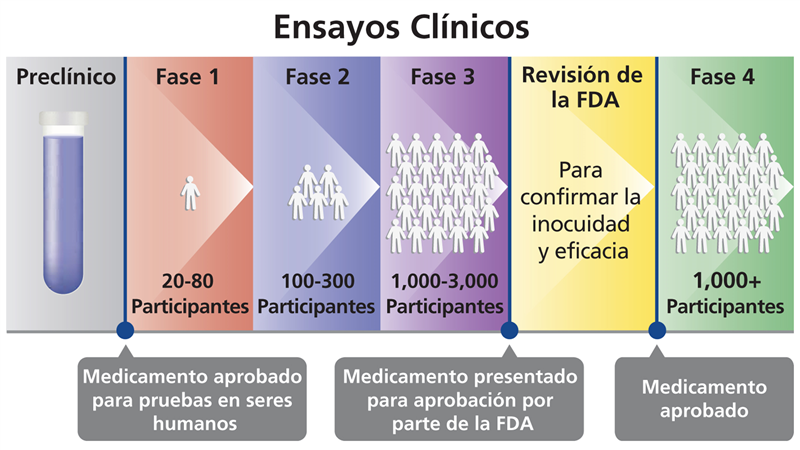
\includegraphics[width=0.8\linewidth]{INREMDN_files/figure-html/ensayosclinicos} 

}

\caption{Fases de los ensayos farmacológicos; fuente: https://clinicalinfo.hiv.gov/es/glossary/ensayo-clinico}\label{fig:ensayosclinicos}
\end{figure}

\begin{itemize}
\item
  Los \textbf{ensayos de fase I} se centran en la pregunta \textbf{¿Es seguro el tratamiento?}. En ellos se prueba el fármaco en grupos pequeños (digamos, de decenas) de voluntarios no necesariamente enfermos, sin grupo de control. Estos ensayos aportan datos preliminares sobre su toxicidad y efectividad en diferentes dosis.
\item
  Los \textbf{ensayos de fase II} se centran en la pregunta \textbf{¿Es efectivo el tratamiento?}. En ellos se prueba el fármaco sobre un grupo de tamaño medio (digamos, de centenares) de enfermos y se comparan los resultados con un grupo de control, pero posiblemente sin aleatorizar los tratamientos. En los ensayos de una vacuna, se prueba sobre todos los sujetos de la muestra, sin grupo de control. Se estudia la eficacia del medicamento (relación dosis/respuesta, dosis óptima, margen de seguridad\ldots.) y los efectos adversos a corto plazo en diferentes condiciones ``de laboratorio'', seguramente diferentes de lo que va a ser su administración habitual si se aprueba el fármaco.
\item
  Los \textbf{ensayos de fase III} se centran en la pregunta \textbf{¿Es mejor el nuevo tratamiento que el convencional?} Se trata de ensayos controlados aleatorizados sobre un grupo de enfermos mucho mayor (digamos, de miles) en los que se evalúa la eficacia del medicamento en condiciones de uso similares a las que se darían cuando se hubiera aprobado, así como su seguridad a más largo plazo, comparándolo con las alternativas terapéuticas disponibles.
\item
  Los \textbf{ensayos de fase IV} se llevan a cabo tras la comercialización y varios años de uso del fármaco. En ellos se revalúa su efectividad y se estudian sus posibles nuevas indicaciones y su seguridad a largo plazo.
\end{itemize}

\hypertarget{a-modo-de-resumen}{%
\section{A modo de resumen}\label{a-modo-de-resumen}}

El gráfico siguiente presenta un diagrama de flujo para clasificar un estudio médico en los diferentes tipos explicados hasta el momento.

\begin{figure}

{\centering 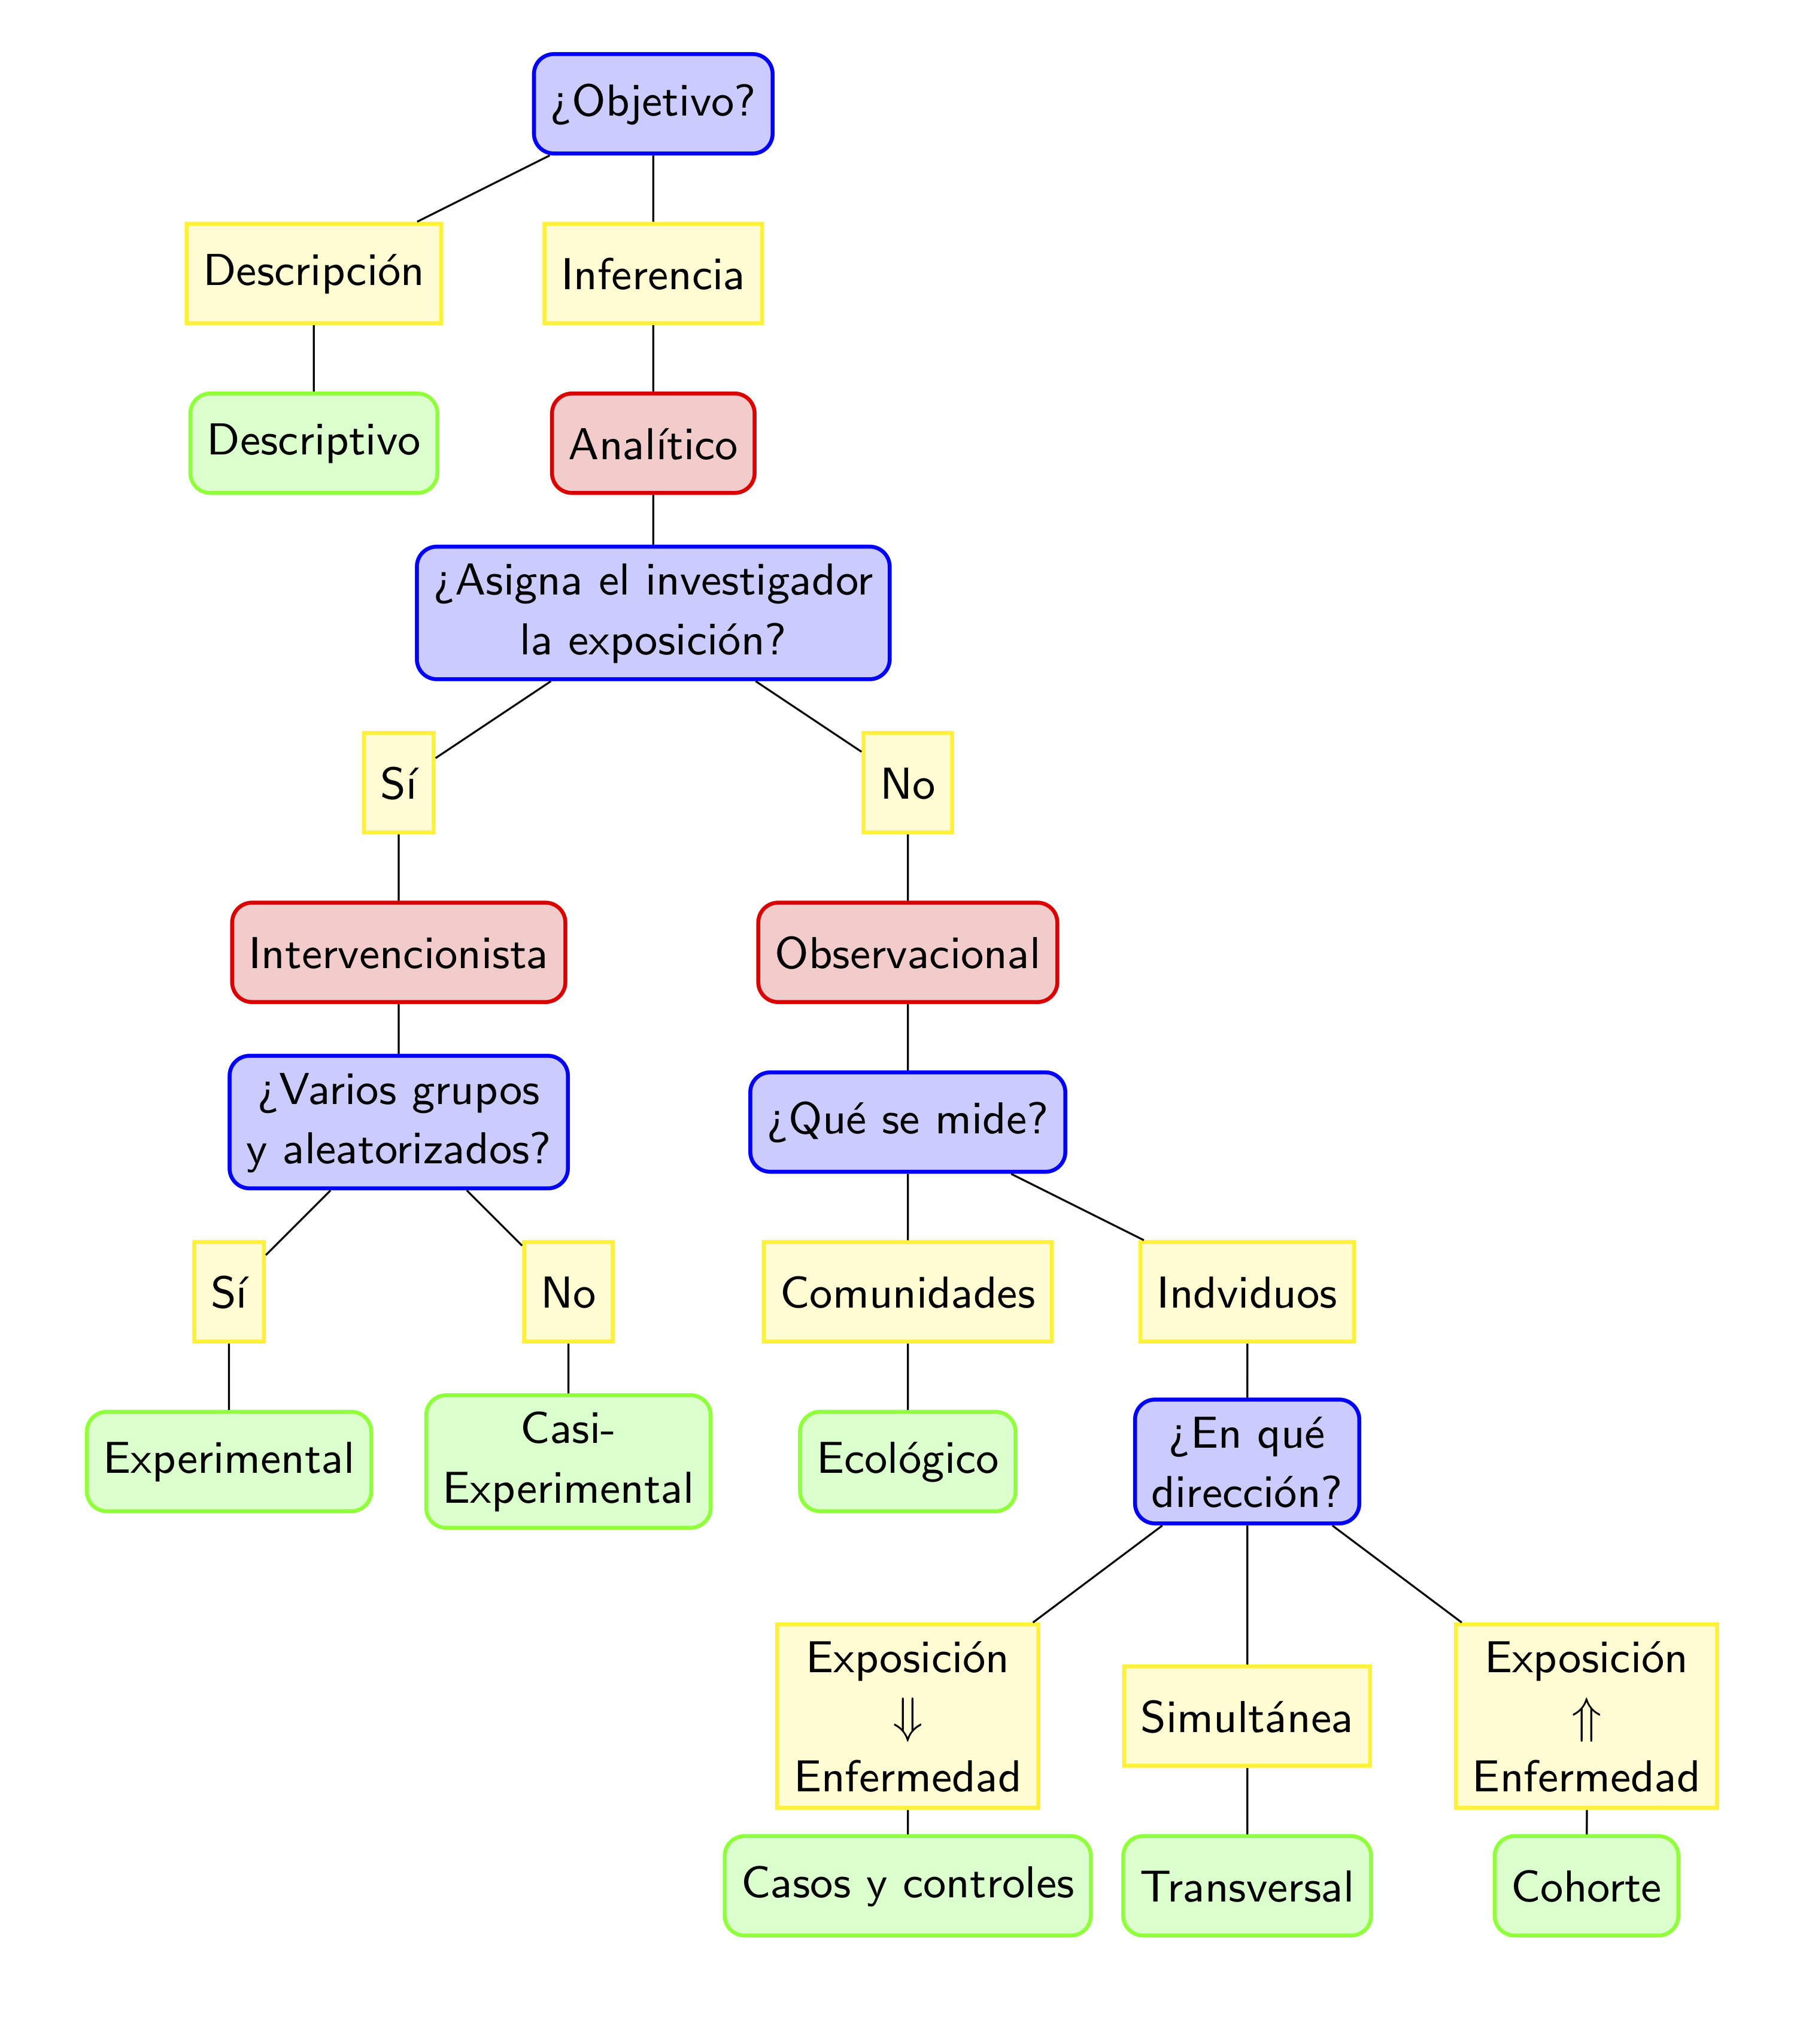
\includegraphics[width=0.9\linewidth]{INREMDN_files/figure-html/estructura} 

}

\caption{Algoritmo para la clasificación básica de un estudio médico.}\label{fig:algoritmo}
\end{figure}

Hay muchos más tipos de estudios médicos: estudios híbridos que mezclan aspectos de diferentes tipos (casos-cohorte, casos y controles anidados en una cohorte, estudios casi-experimentales con un control externo,\ldots), estudios secuenciales (en los que se analizan cada cierto tiempo los resultados obtenidos y se decide si se continua el estudio ampliando la muestra o si se para antes de su final previsto), etc. No los vamos a estudiar en este curso.

\hypertarget{revisiones-sistemuxe1ticas-y-metaanuxe1lisis}{%
\section{Revisiones sistemáticas y metaanálisis}\label{revisiones-sistemuxe1ticas-y-metaanuxe1lisis}}

Hay un último tipo de estudios que queremos comentar, en los que las muestras que se estudian están formadas por \ldots{} estudios médicos previos sobre un tema. Se trata de las \textbf{revisiones sistemáticas}: Resúmenes de todo lo publicado sobre un tema específico. Entre las revisiones sistemáticas, aquí destacamos los \textbf{metaanálisis}, que usan técnicas estadísticas para analizar conjuntamente los resultados publicados en una serie de estudios previos sobre un tema concreto.

\begin{rmdnote}
Observad que si se han efectuado, digamos, 25 estudios sobre un tema y en cada uno han participado, pongamos, 40 sujetos, al analizar conjuntamente los datos generados es como si se tratara de un estudio con 1000 sujetos. Como os podéis imaginar, las conclusiones que se obtienen a partir de 1000 sujetos son más fiables que las que se obtienen con 40. De hecho, son más fiables que las que se obtienen en 25 estudios con 40 participantes cada uno, como veremos más adelante en el tema de Contrastes de Hipótesis.
\end{rmdnote}

\begin{figure}

{\centering 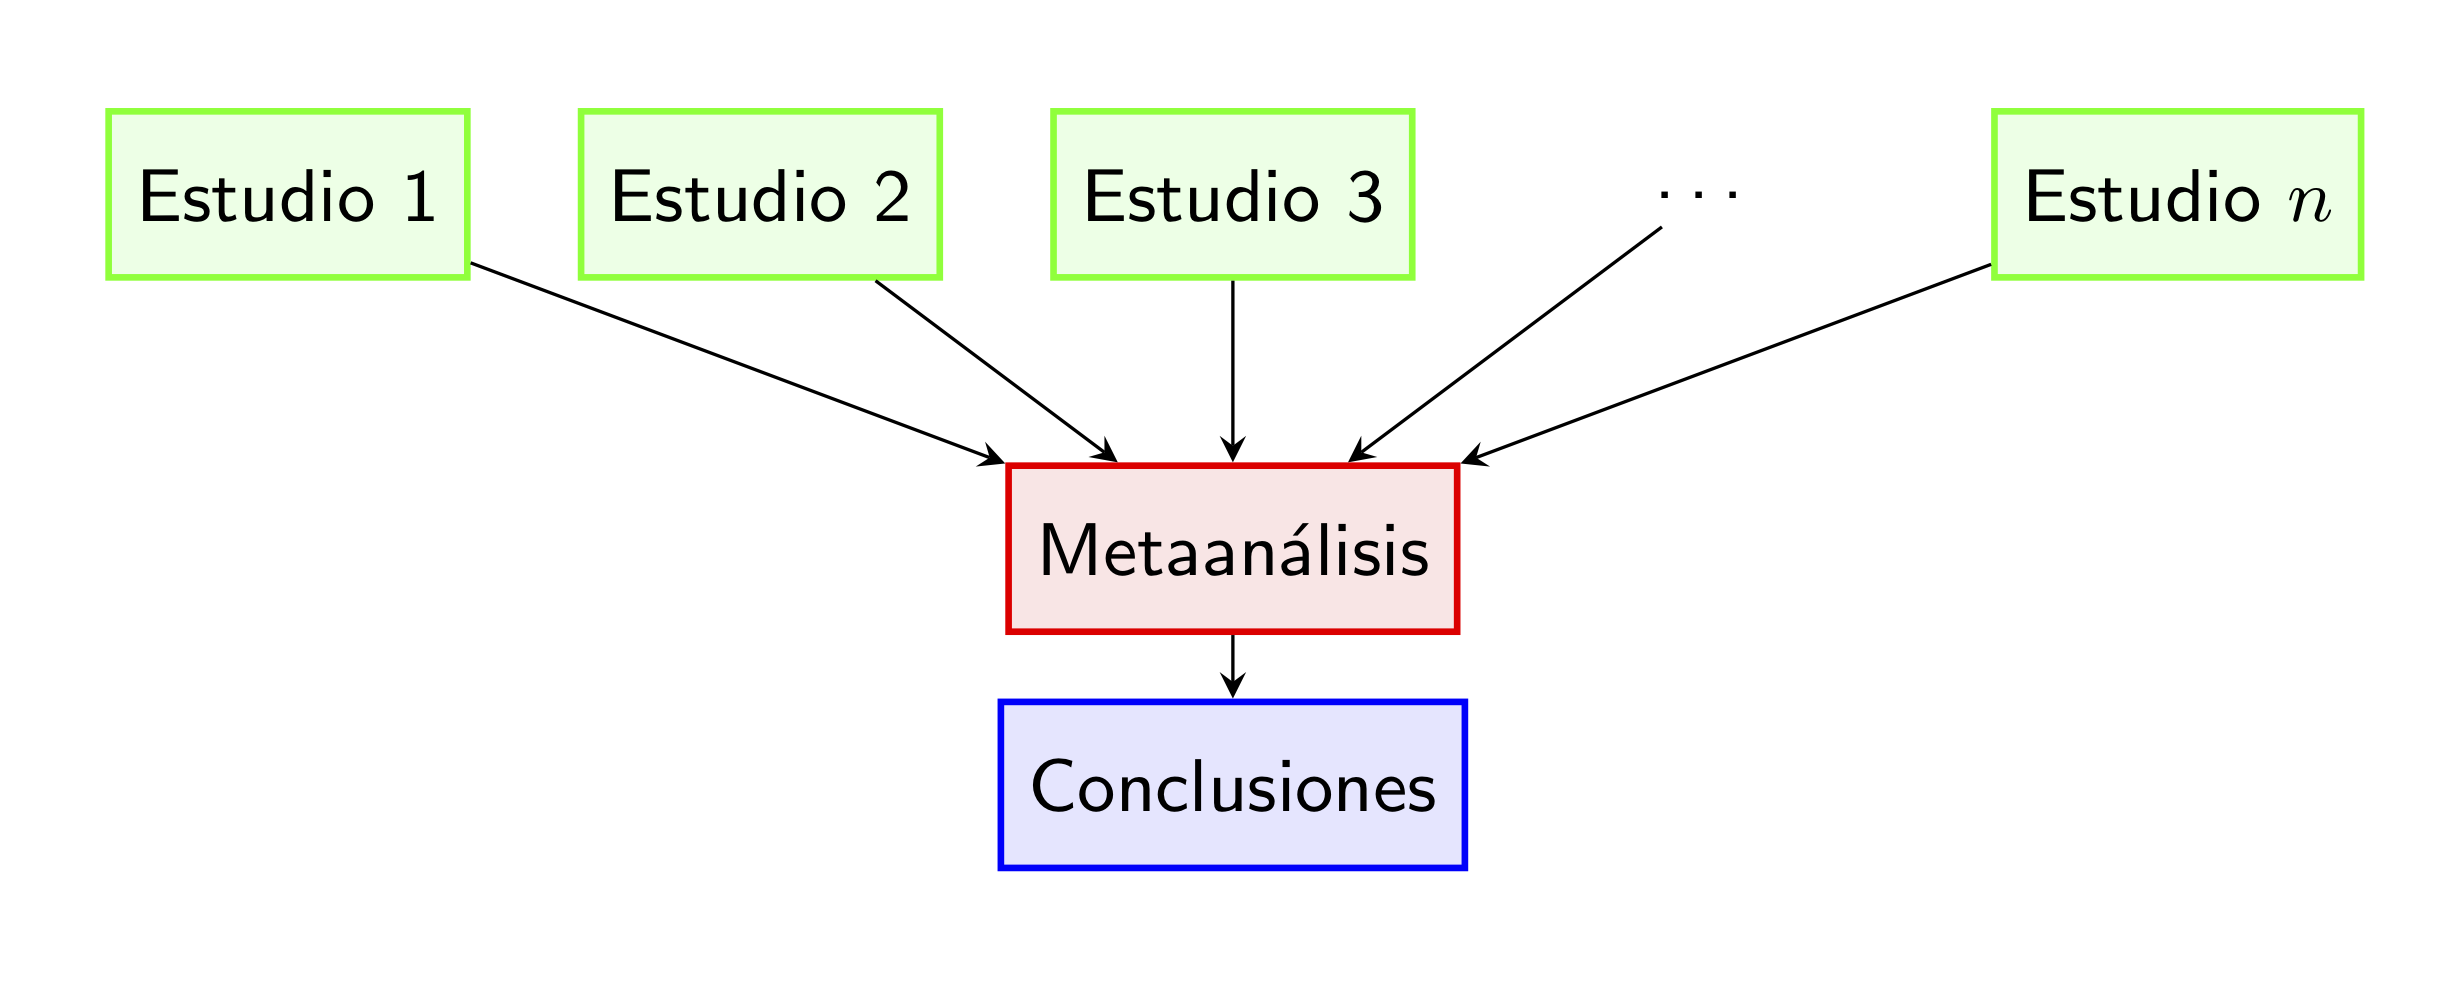
\includegraphics[width=0.8\linewidth]{INREMDN_files/figure-html/metaanalisis} 

}

\caption{Esquema de un metaanálisis.}\label{fig:metaanálisis}
\end{figure}

\begin{example}
\protect\hypertarget{exm:acné}{}\label{exm:acné}En el estudio \href{https://www.sciencedirect.com/science/article/pii/S0009741115002364}{``¿Resistencia en el acné? Un metaanálisis a propósito de la controversia''} (M. Álvarez-Sánchez \emph{et al}, \emph{Cirugía y Cirujanos} 84 (2016), pp.~190-195), se presenta un metaanálisis de las publicaciones de los 10 años anteriores a su aparición sobre la resistencia bacteriana del \emph{Propionibacterium acnes} a los antibióticos tópicos usados habitualmente en el tratamiento del acné.
\end{example}

En primer lugar, se hizo una selección sistemática de aquellos estudios que iban a ser incorporados al metaanálisis, que al final fueron solo 13 de 501 candidatos, según el proceso descrito en el \textbf{flujograma} siguiente:

\begin{figure}

{\centering 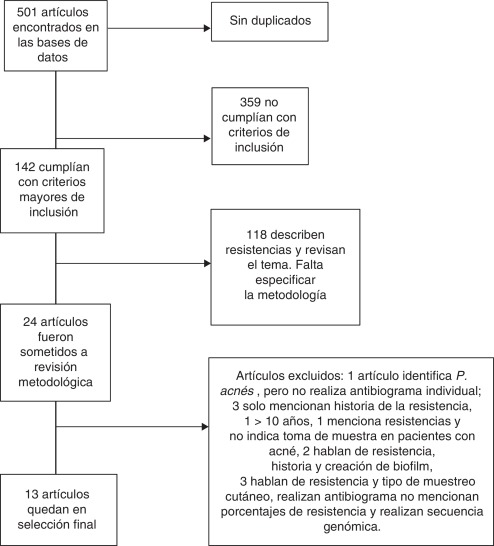
\includegraphics[width=0.9\linewidth]{INREMDN_files/figure-html/acne2} 

}

\caption{Proceso de selección de los artículos en el estudio sobre resistencia en el acné (Figura 2 en el artículo).}\label{fig:acne2}
\end{figure}

De los 13 estudios analizados, en 8 se había obtenido evidencia de un aumento en la resistencia del \emph{P. acnes} a la eritromicina y clindamicina tópicas usadas en tratamientos anti acné, de los cuales solo en 1 fue significativo, y en 5 se obtuvo evidencia de un aumento en su sensibilidad, de los cuales en 2 fue significativo. Al analizar conjuntamente los datos de los 13 estudios, se obtuvo evidencia de que ha habido un aumento en la resistencia del \emph{P. acnes} a estos antibióticos, pero el aumento detectado no fue significativo.

\begin{figure}

{\centering 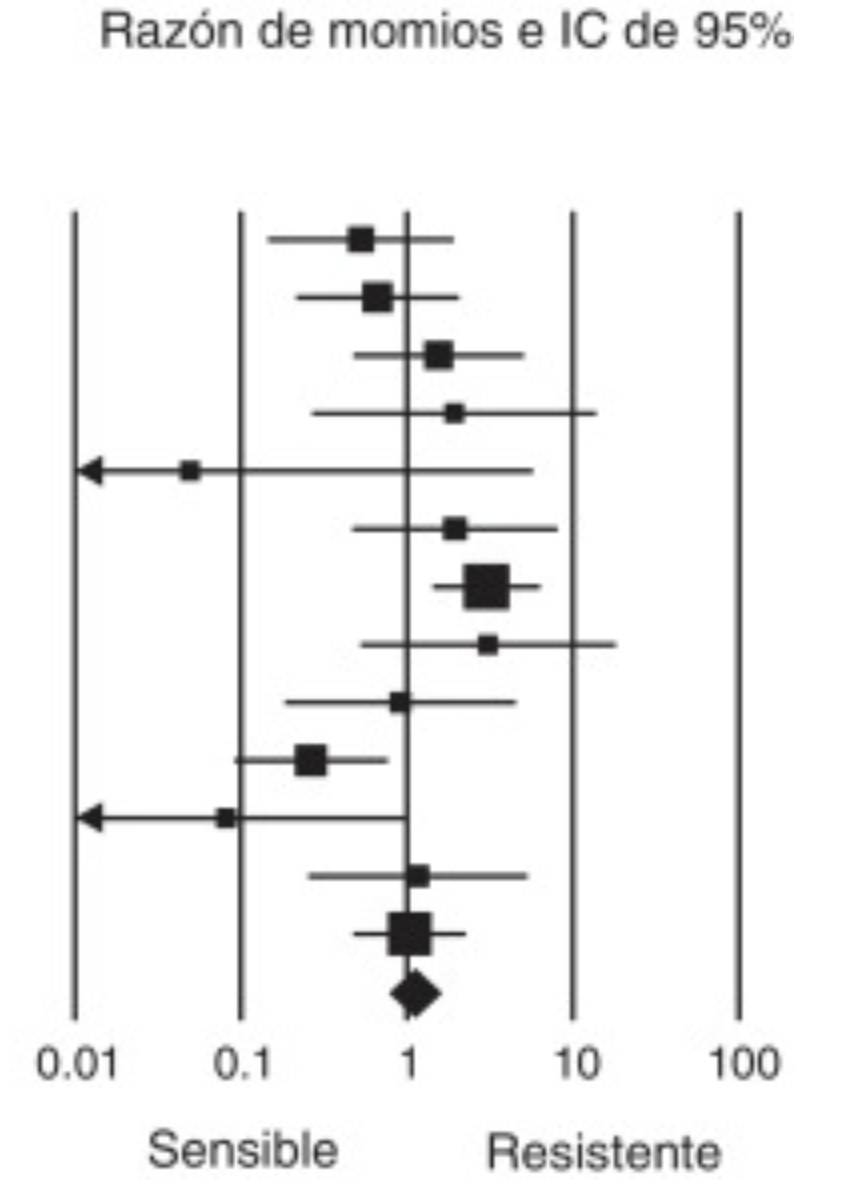
\includegraphics[width=0.4\linewidth]{INREMDN_files/figure-html/blob} 

}

\caption{Forest plot del estudio sobre resistencia en el acné (Figura 1 en el artículo).}\label{fig:blob}
\end{figure}

Los resultados de un metaanálisis se suelen representar mediante un \textbf{forest plot} (o también \textbf{diagrama de efectos} o \textbf{blobograma}) como el de la Figura \ref{fig:blob}. Sobre este diagrama conviene saber que:

\begin{itemize}
\item
  Los segmentos con un cuadrado en su centro representan los estudios analizados. Para cada uno de estos estudios y segmentos:

  \begin{itemize}
  \tightlist
  \item
    El tamaño del cuadrado representa (en este ejemplo) el tamaño de la muestra usada
  \item
    La posición del centro del cuadrado representa el valor estimado del aumento del riesgo de resistencia (medido mediante la \emph{odds ratio}, o razón de momios, del título del gráfico, de la que hablaremos en la Sección \ref{sec:odds}). Si el centro está en la zona ``Sensible'' (a la izquierda de 1), en el estudio se observó un aumento de la sensibilidad, mientras que si el centro está en de la zona ``Resistente'' (a la derecha de 1), se observó un aumento de la resistencia.
  \item
    La longitud del segmento representa la incertidumbre de la generalización de esta estimación al total de la población (fijaos en que a mayor tamaño de la muestra, menor incertidumbre); formalmente, se tratan de \textbf{intervalos de confianza del 95\%} (Sección \ref{sec:IC})
  \item
    Si el segmento está totalmente contenido de la zona ``Sensible'', se obtuvo \textbf{evidencia significativa} de aumento de la sensibilidad, mientras que si el intervalo está totalmente contenido de la zona ``Resistente'', se obtuvo \textbf{evidencia significativa} de aumento de la resistencia. Si el segmento curta la línea vertical del 1, la evidencia obtenida no fue significativa.
  \end{itemize}
\item
  Els segmento con un rombo en su centro representa el resultado del metaanálisis. Su interpretación es la misma que para los anteriores. Como su centro está en la zona ``Resistente'', se obtuvo evidencia de aumento en la resistencia, pero como cruza la línea vertical del 1, la evidencia no fue significativa.
\end{itemize}

La Figura \ref{fig:piramide} representa la llamada \textbf{pirámide de la evidencia}, que ordena los tipos de estudio, de la base hacia la cúspide, en función de la calidad de la evidencia científica que, en general, aportan. Cuanto más arriba en la pirámide está un tipo de estudio, en principio con más seguridad se pueden adoptar sus conclusiones en la práctica médica. Si reflexionáis un poco, veréis que el orden que describe es muy razonable.

\begin{figure}

{\centering 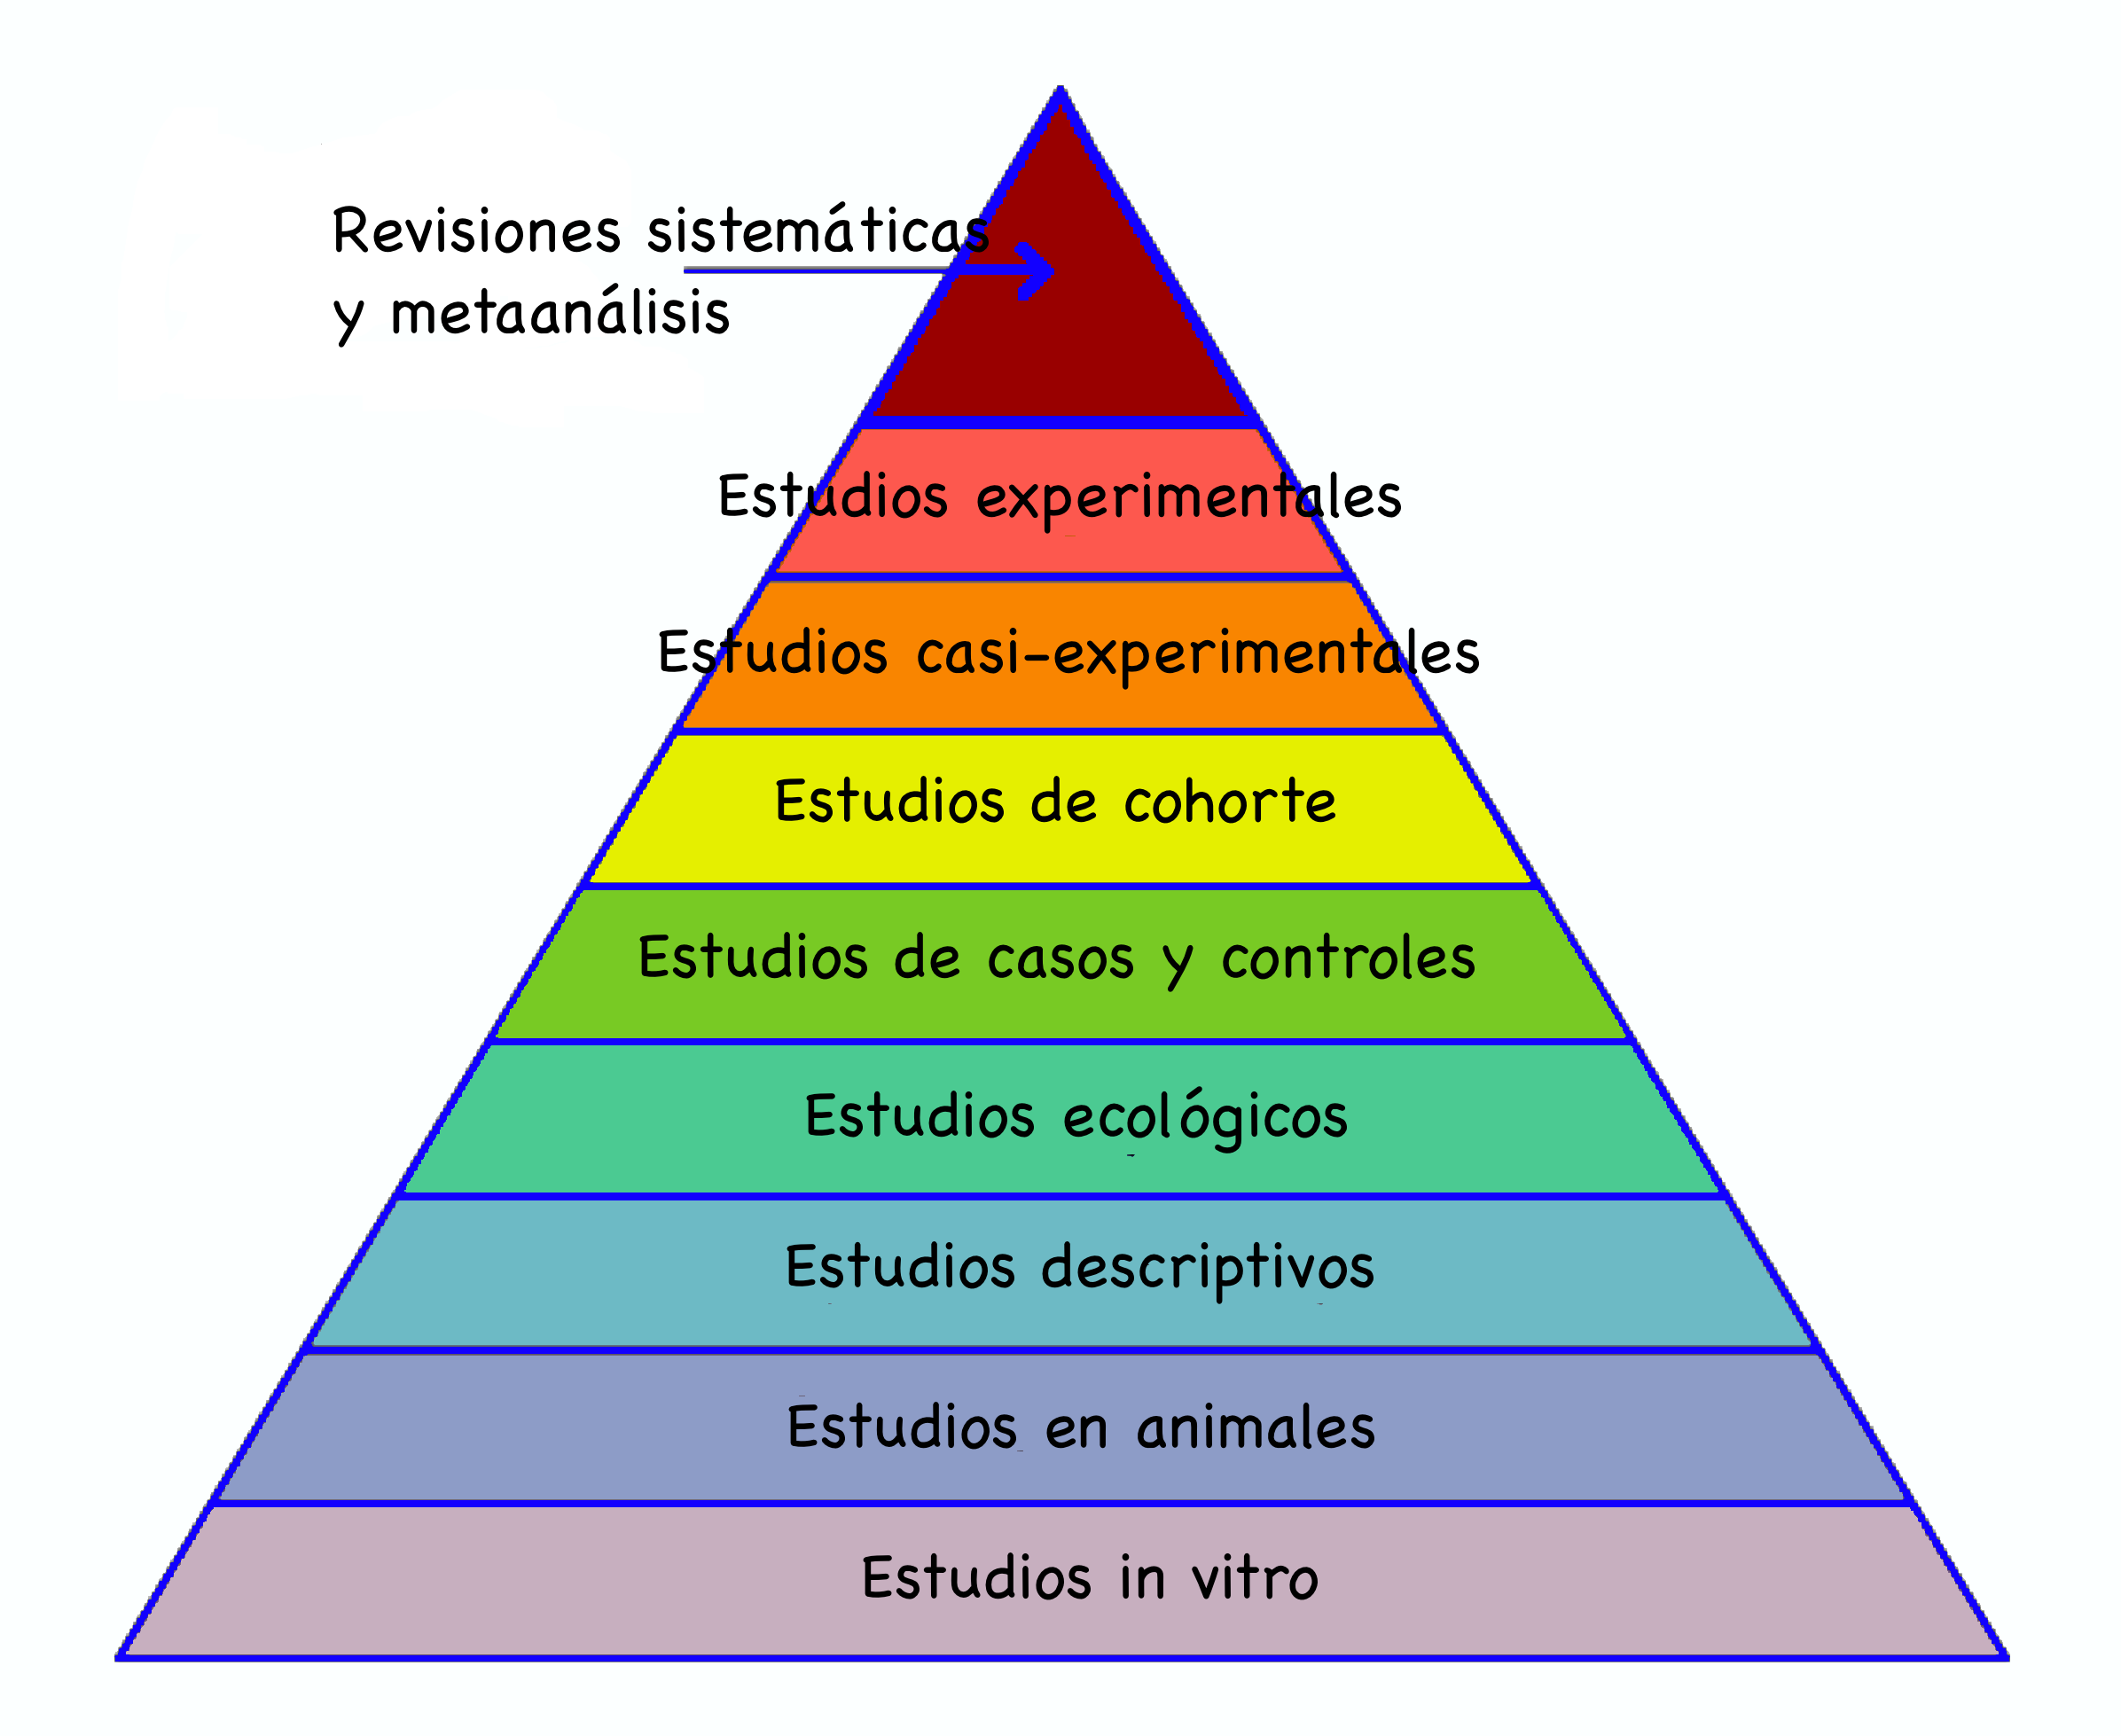
\includegraphics[width=0.8\linewidth]{INREMDN_files/figure-html/systematic} 

}

\caption{Pirámide de la evidencia.}\label{fig:piramide}
\end{figure}

Los metaanálisis representan la cúspide de la evidencia en estudios médicos, pero no están exentos de problemas:

\begin{itemize}
\item
  Son sensibles al \textbf{sesgo de publicación}. Se tiende a publicar en revistas científicas solo aquellos estudios que presentan resultados positivos o al menos ``interesantes''; las revistas científicas son un negocio, y la mayoría solo publican los artículos que puedan hacer crecer su prestigio y con él las ventas. Por este motivo, si solo se tienen en cuenta estudios publicados en revistas, las conclusiones pueden estar sesgadas. Es imprescindible buscar, e incluir, posibles estudios que hayan quedado sin publicar porque no obtuviesen evidencia significativa de nada.
\item
  Si los estudios analizados son defectuosos, el metaanálisis no los salva, y las conclusiones pueden ser erróneas. Por ello es necesario establecer unos criterios precisos de calidad de los estudios cuyos datos se vayan a tener en cuenta.
\end{itemize}

\hypertarget{sec:causalidad}{%
\section{(Bonus track) Unos criterios de causalidad}\label{sec:causalidad}}

El objetivo final de la mayoría de estudios médicos es establecer una relación de \textbf{causalidad}, de causa/efecto:

\begin{itemize}
\tightlist
\item
  Esta medicina cura esta enfermedad.
\item
  La exposición a tal riesgo aumenta el riesgo de padecer esta enfermedad.
\item
  Esta vacuna previene esta enfermedad.
\item
  Etc.
\end{itemize}

Por desgracia, como ya hemos comentado, es virtualmente imposible establecer sin ninguna duda una relación de causalidad entre dos eventos por medio de un estudio médico. Por ejemplo, ¿cómo podríamos estar absolutamente seguros de que fumar aumenta el riesgo de cáncer de pulmón? Pues la única manera sería tomar un grupo de personas, hacerles fumar cantidades fijas de cigarrillos diarios y anotar quiénes de ellos desarrollan cáncer de pulmón a lo largo de su vida. A continuación, volver atrás en el tiempo, impedirles totalmente que fumen, hacerles revivir su vida exactamente como en la primera ronda salvo por el hecho de que ahora no fuman (su vida, y la del resto del universo, fluctuaciones cuánticas incluidas), y anotar quiénes desarrollan cáncer de pulmón en esta segunda oportunidad. Solo de esta manera garantizaríamos que cualquier diferencia en los números de cáncer de pulmón se debe al fumar.

Como no podemos usar esta técnica, hemos de echar mano a estudios como los explicados en las secciones anteriores, que en general solo muestran una asociación entre una exposición y un desenlace y en los que no podemos controlar todas las variables que puedan influir en el desenlace, incluyendo confundidores. Cierto es que en los estudios experimentales las controlamos más que en el resto, pero no al cien por cien. En estas condiciones, está claro que la asociación que se observe no tiene por qué implicar causalidad.

\begin{example}
\protect\hypertarget{exm:univturmor}{}\label{exm:univturmor}En el estudio \href{https://jech.bmj.com/content/70/12/1222}{``Socioeconomic position and the risk of brain tumour: a Swedish national population-based cohort study''} (A. Khanolkar \emph{et al}, \emph{Journal of Epidemiology and Community Health} 70 (2016), pp.~1222-1228) se realizó un seguimiento durante 17 años a más de 4 millones de suecos, y se observó una asociación sorprendente: los que habían cursado al menos 3 años de estudios universitarios tenían un 22\% más de probabilidad de tener un glioma (un tipo de tumor cerebral) que los que solo tenían educación primaria. La diferencia fue además estadísticamente significativa. ¿Creéis que puede ser verdad que tener estudios universitarios cause un aumento de la probabilidad de tener un glioma?
\end{example}

Seguramente no. Incluso los autores lo reconocen en sus Conclusiones. En lo que se detectó una diferencia significativa fue en \textbf{el número de diagnósticos de glioma}, que pudo deberse a que las personas con estudios superiores tienen una mayor probabilidad de que su glioma sea detectado, por ejemplo porque acudan al médico antes, y que sea registrado en el Registro Nacional de Cáncer, que es de donde se extrajo la información sobre los cánceres. Naturalmente, en el periódico solo vais a encontrar la parte llamativa del estudio, como muestra el titular de la noticia del ABC sobre el tema.

\begin{figure}

{\centering 
\includegraphics[width=0.8\linewidth]{INREMDN_files/figure-html/ABCglioma} 

}

\caption{Noticia publicada en el ABC el 21 junio de 2016. El texto completo está disponible en https://www.abc.es/salud/enfermedades/abci-estudios-universitarios-podrian-aumentar-riesgo-tumores-cerebrales-201606201751_noticia.html.}\label{fig:ABCglioma}
\end{figure}

El estadístico \href{https://es.wikipedia.org/wiki/Austin_Bradford_Hill}{Austin Bradford Hill} (que ya ha aparecido en esta lección como coautor del estudio pionero sobre cáncer y tabaco del Ejemplo \ref{exm:rubeola}) enunció la lista más popular de criterios de causalidad para poder aceptar que una asociación observada entre una exposición y un desenlace sea en realidad una relación causal. El primer criterio es obvio, y el único que es necesario que se cumpla:

\begin{itemize}
\tightlist
\item
  \textbf{Temporalidad}: La pretendida causa tiene que preceder temporalmente al efecto.
\end{itemize}

El resto de criterios son optativos, pero cuantos más se cumplan, más fuerza tiene el argumento en favor de la relación causa/efecto. Vamos a ilustrarlos con argumentos en favor de que niveles altos de colesterol en sangre aumentan el riesgo de enfermedad coronaria.

\begin{itemize}
\item
  \textbf{Fuerza de la asociación estadística}: Cuanto mayor sea la asociación observada (en el sentido, por ejemplo, de cuántas veces mayor es la frecuencia observada del desenlace entre los expuestos que entre los no expuestos), más creíble es que la exposición sea la causa del desenlace.

  Por ejemplo, ha habido estudios de cohorte en los que se ha observado un aumento de casi un 300\% en la incidencia de enfermedades coronarias entre los sujetos con nivel muy alto de colesterol respecto de los sujetos con niveles normales.
\item
  \textbf{Consistencia} o \textbf{reproducibilidad}: Si cada vez que se llevan a cabo estudios similares se obtienen conclusiones similares, es más creíble que la relación causal sea verdadera.

  La asociación entre niveles altos de colesterol y enfermedades coronarias se ha observado en multitud de estudios tanto de casos y controles como de cohorte sobre poblaciones de características diferentes.
\item
  \textbf{Plausibilidad biológica}: La existencia de una explicación biológica plausible de la relación causa/efecto hace más creíble que esta relación sea verdadera.

  Se ha comprobado que el colesterol LDL promueve el desarrollo de placas arterioescleróticas, y estas aparecen en las enfermedades cardíacas.
\item
  \textbf{Coherencia}: Si la relación causa/efecto propuesta no va contra el conocimiento científico sobre el tema, es más creíble que sea verdadera.

  Fijaos en que no es lo mismo tener una explicación biológica para la causalidad (el criterio anterior) que la ausencia de teorías o estudios que la contradigan. En nuestro caso, la asociación entre el colesterol y la enfermedad cardíaca no contradice ningún estudio conocido ni ningún mecanismo biológico conocido.
\item
  \textbf{Especificidad}: Si se han descartado mediante otros estudios otras posibles causas del desenlace, aumenta la verosimilitud de que la exposición para la que sí se ha encontrado una asociación lo cause.

  La asociación entre colesterol alto y el desarrollo de enfermedades cardíacas se ha mantenido cuando se han descartado los efectos de posibles confundidores como el tabaco, el alcohol, la edad, la tensión arterial etc.
\item
  \textbf{Relación dosis-respuesta}: Si a mayor exposición se observa una mayor frecuencia de aparición del desenlace, es más creíble que la exposición sea la causa del desenlace.

  En el ejemplo que nos ocupa, se ha observado en muchos estudios que la probabilidad de tener una enfermedad cardíaca crece con el nivel de colesterol.
\item
  \textbf{Reversibilidad}: Si se observa que el desenlace tiende a desaparecer al eliminar la exposición, es más creíble que la exposición sea la causa del desenlace.

  Se han realizado estudios experimentales en los que se ha observado que si se reduce el nivel de colesterol por medio de la administración de fármacos, se reduce la riesgo de enfermedad coronaria.
\item
  \textbf{Calidad del estudio}: La relación causa/efecto es más creíble si la asociación se ha establecido en un estudio experimental que si lo ha sido en estudios inferiores en la pirámide de la evidencia.

  Naturalmente, en nuestro ejemplo no se han llevado a cabo estudios experimentales en los que a sujetos se les aumentara el nivel de colesterol para ver si tenían un infarto, pero como hemos comentado sí que se han realizado en el sentido contrario.
\item
  \textbf{Analogía}: Si se ha aceptado que exposiciones similares causan desenlaces similares, es más fácil de aceptar que esta relación causa/efecto se dé también en nuestro caso.

  Se han descrito mecanismos similares al relacionado con el colesterol LDL que producen placas arterioescleróticas.
\end{itemize}

\hypertarget{bonus-track-preguntas-cluxednicas-en-formato-pico}{%
\section{(Bonus track) Preguntas clínicas en formato PICO}\label{bonus-track-preguntas-cluxednicas-en-formato-pico}}

Al buscar información sobre un tema médico específico, es importante formular la pregunta de manera adecuada. Un esquema muy usado para estructurar este tipo de preguntas es el \textbf{PICO}, acrónimo de \textbf{P}aciente-\textbf{I}ntervención-\textbf{C}omparación-\textbf{O}\emph{utcome} (resultado):

\begin{itemize}
\item
  ¿Sobre qué tipo de \textbf{P}aciente? Se trata de especificar con precisión el tipo de paciente (o de \textbf{P}ersona, si está sano) sobre el que nos interesa obtener información.
\item
  ¿Qué \textbf{I}ntervención? Aquí \textbf{intervención} puede referir a un tratamiento de una enfermedad, la exposición a un factor de riesgo, una prueba diagnóstica\ldots{}
\item
  ¿\textbf{C}omparado con qué otra intervención? A veces esta parte no se tiene en cuenta, si no se quiere comparar el resultado de la intervención con nada sino simplemente saber su resultado. Hablaríamos entonces del formato \textbf{PIO}.
\item
  ¿Qué resultado (\textbf{O}\emph{utcome}) nos interesa? Aquí \textbf{resultado} refiere a las consecuencias de la intervención en la salud del paciente.
\end{itemize}

\begin{example}
\protect\hypertarget{exm:unnamed-chunk-55}{}\label{exm:unnamed-chunk-55}Vamos a traducir al formato PICO la pregunta ``¿El uso de ácido acetil salicílico (AAS), aumenta la supervivencia en el infarto agudo de miocardio?''
\end{example}

\begin{itemize}
\item
  \textbf{P}aciente. ¿Ante qué tipo de pacientes se nos plantea el problema? No vale ``las personas en general''. Por ejemplo, podría ser:

  \begin{itemize}
  \tightlist
  \item
    En los pacientes mayores de 60 años con síndrome coronario agudo con \href{http://www.medintensiva.org/es/significado-clinico-del-sindrome-coronario/articulo/S0210569111000866/}{elevación del ST}\ldots{}
  \end{itemize}
\item
  \textbf{I}ntervención. ¿De qué tipo de acción queremos saber las consecuencias?

  \begin{itemize}
  \tightlist
  \item
    \ldots{} la administración de AAS\ldots{}
  \end{itemize}
\item
  \textbf{C}omparación. ¿Con respecto a qué queremos comparar la intervención?

  \begin{itemize}
  \tightlist
  \item
    \ldots{} con respecto a no administrarles nada\ldots{}
  \end{itemize}
\item
  \textbf{O}\emph{utcome} (Resultado). ¿En qué efecto estamos interesados? Como a la larga nadie sobrevive a la vida, podría ser, por ejemplo
\item
  \ldots{} ¿aumenta la tasa de supervivencia a 30 días vista?
\end{itemize}

Nos quedaría:

\begin{quote}
En los pacientes mayores de 60 años con síndrome coronario agudo con elevación del ST, ¿la administración de AAS aumenta la tasa de supervivencia a los 30 días con respecto a no administrarles nada?
\end{quote}

\begin{example}
\protect\hypertarget{exm:unnamed-chunk-56}{}\label{exm:unnamed-chunk-56}Considerad la situación siguiente. X es una nueva paciente de 76 años que acude a vuestra consulta para hacerse un examen físico periódico. X se encuentra en buen estado de salud aunque sufre de hipertensión desde hace muchos años. Su hipertensión está controlada con éxito mediante beta-bloqueantes y nos ha expresado su satisfacción con esta terapia. Sin embargo, su hijo ha sido diagnosticado recientemente de hipertensión y se le ha recetado un \href{https://es.wikipedia.org/wiki/Inhibidor_de_la_enzima_convertidora_de_angiotensina}{inhibidor de la ECA}. X os pregunta si este tratamiento sería una mejor opción para ella.

Vamos a traducir la pregunta planteada por X al formato PICO.
\end{example}

\begin{itemize}
\tightlist
\item
  \textbf{P}: mujer, edad avanzada, hipertensa, por lo demás en buen estado de salud
\item
  \textbf{I}: administrar un inhibidor de la ECA
\item
  \textbf{C}: administrar beta-bloqueantes
\item
  \textbf{O}: eficacia en la reducción de la presión arterial, efectos secundarios.
\end{itemize}

Como resultado, la pregunta PICO podría ser:

\begin{quote}
En mujeres hipertensas de edad avanzada, ¿un inhibidor de la ECA es más eficaz que un beta-bloqueante para controlar la presión arterial alta y minimizar los efectos secundarios adversos?
\end{quote}

\hypertarget{test}{%
\section{Test}\label{test}}

\textbf{(1)} Un estudio publicado describe varias características de los pacientes ingresados con neumonía en un hospital durante un año, incluidos el sexo, la edad, el historial de tabaquismo y el historial de ingresos previos por neumonía. ¿De qué tipo de estudio se trata?

\begin{enumerate}
\def\labelenumi{\arabic{enumi}.}
\tightlist
\item
  Descriptivo
\item
  Transversal
\item
  De cohorte prospectivo
\item
  De cohorte retrospectivo
\item
  De casos y controles
\end{enumerate}

\textbf{(2)} En un artículo publicado se estudió a pacientes atendidos en una clínica por apendicitis aguda tratada con apendicectomía laparoscópica.
Se tomaron 50 de ellos que presentaron infección de la herida una semana después del alta y 50 que no la presentaron. El estudio comparó entre ambos grupos los factores que se anotaron en el ingreso, como la edad, el sexo, la presencia de dolor en el cuadrante inferior derecho, la temperatura, entre otros. El objetivo era determinar cuáles influyen en la aparición de la infección. ¿De qué tipo de estudio se trata?

\begin{enumerate}
\def\labelenumi{\arabic{enumi}.}
\tightlist
\item
  Descriptivo
\item
  Transversal
\item
  De cohorte prospectivo
\item
  De cohorte retrospectivo
\item
  De casos y controles
\end{enumerate}

\textbf{(3)} Si identificamos pacientes con bronquitis crónica obstructiva en el año 2010 tratados y no tratados con corticoides por vía inhalatoria, y comparamos su función respiratoria a día de hoy, se trata de un estudio:

\begin{enumerate}
\def\labelenumi{\arabic{enumi}.}
\tightlist
\item
  Descriptivo
\item
  Transversal
\item
  De cohorte prospectivo
\item
  De cohorte retrospectivo
\item
  De casos y controles
\end{enumerate}

\textbf{(4)} Se ha llevado a cabo un estudio con el fin de determinar el riesgo de hemorragia digestiva alta (HDA) asociado con el uso de diferentes anti-inflamatorios no esteroideos (AINE). Para ello se incluyeron 2777 pacientes con HDA y 5532 pacientes emparejados con los anteriores por edad y mes de ingreso o consulta en los mismos hospitales, pero por otras razones que no tuvieran que ver con el uso de AINE. Se comparó la exposición previa a diferentes AINE en ambos grupos. ¿De qué tipo de estudio se trata?

\begin{enumerate}
\def\labelenumi{\arabic{enumi}.}
\tightlist
\item
  Descriptivo
\item
  Transversal
\item
  De cohorte prospectivo
\item
  De cohorte retrospectivo
\item
  De casos y controles
\item
  Intervencionista
\item
  Ecológico
\end{enumerate}

\textbf{(5)} Que un ensayo clínico sea ``abierto'' significa que:

\begin{enumerate}
\def\labelenumi{\arabic{enumi}.}
\tightlist
\item
  No requiere ingreso.
\item
  Pueden incluirse sujetos en el ensayo una vez iniciado.
\item
  No existe grupo control.
\item
  No es enmascarado.
\item
  Sus resultados son extrapolables a la población general.
\end{enumerate}

\textbf{(6)} En un centro de salud se está realizando un estudio para determinar el efecto de la exposición al humo del tabaco en hijos de padres fumadores. Para ello, se selecciona a un grupo de niños sanos entre 3 y 7 años cuyos padres son fumadores y al mismo tiempo se selecciona en el mismo centro un número igual de niños cuyos padres no son fumadores. Un año después se investigará en ambos grupos la aparición de enfermedades respiratorias durante ese año. ¿De qué tipo de estudio se trata?

\begin{enumerate}
\def\labelenumi{\arabic{enumi}.}
\tightlist
\item
  Descriptivo
\item
  Transversal
\item
  De cohorte prospectivo
\item
  De cohorte retrospectivo
\item
  De casos y controles
\item
  Experimental
\item
  Casi-experimental
\item
  Ecológico
\end{enumerate}

\textbf{(7)} En un estudio de fase III destinado a confirmar la eficacia bacteriológica de un nuevo antibiótico para el tratamiento de pacientes con pielonefritis aguda (una infección bacteriana de las vías urinarias que puede desembocar en insuficiencia renal, sepsis\ldots) grave, ¿cuál de los siguientes diseños de ensayo clínico es el más apropiado?

\begin{enumerate}
\def\labelenumi{\arabic{enumi}.}
\tightlist
\item
  Paralelo, abierto, controlado con placebo
\item
  Paralelo, aleatorizado, doble ciego, controlado con otro antibiótico
\item
  Cruzado, abierto, controlado con otro antibiótico
\item
  Cruzado, aleatorizado, doble ciego, controlado con placebo
\end{enumerate}

\textbf{(8)} La medicina basada en la evidencia propone integrar las mejores evidencias con la experiencia clínica y las circunstancias de los pacientes en la toma de las decisiones clínicas. En relación a la calidad de la evidencia, ¿cuál de los siguientes tipos de estudio proporciona evidencias de mayor calidad?:

\begin{enumerate}
\def\labelenumi{\arabic{enumi}.}
\tightlist
\item
  Revisiones sistemáticas
\item
  Estudios de cohorte
\item
  Estudios de casos y controles
\item
  Ensayos clínicos aleatorizados y controlados
\item
  Ensayos clínicos doble ciegos, aleatorizados y controlados con placebo
\end{enumerate}

\textbf{(9)} Seleccionamos una muestra aleatoria entre los pacientes que acuden a vacunarse de la gripe durante la campaña anual en un centro de salud. Se registra en los pacientes seleccionados si están utilizando fármacos hipolipemiantes y si están diagnosticados de diabetes mellitus, entre otros datos. Se obtiene que la diabetes mellitus es más frecuente entre los pacientes que toman hipolipemiantes que entre los que no los toman. ¿A cuál de los siguientes corresponde el diseño de este estudio?

\begin{enumerate}
\def\labelenumi{\arabic{enumi}.}
\tightlist
\item
  Descriptivo
\item
  Transversal
\item
  De cohorte prospectivo
\item
  De cohorte retrospectivo
\item
  De casos y controles
\item
  Experimental
\item
  Ecológico
\end{enumerate}

\textbf{(10)} ¿Qué tipos de estudios permiten estimar la incidencia de una enfermedad? Marca todas las respuestas correctas:

\begin{enumerate}
\def\labelenumi{\arabic{enumi}.}
\tightlist
\item
  Series de casos
\item
  De casos y controles
\item
  De cohorte\\
\item
  Transversales
\end{enumerate}

\textbf{(11)} El servicio de dermatología de un hospital ha registrado durante los últimos 20 años todos los casos diagnosticados de necrosis epidérmica tóxica en el centro. Se encuentra que un 20\% de estos pacientes habían estado expuestos a carbamazepina en las 6 semanas previas al diagnóstico, mientras que un 10\% habían estado expuestos a fenitoína. ¿A cuál de los siguientes corresponde el diseño de este estudio?

\begin{enumerate}
\def\labelenumi{\arabic{enumi}.}
\tightlist
\item
  Serie de casos
\item
  Transversal
\item
  De cohorte prospectivo
\item
  De cohorte retrospectivo
\item
  De casos y controles
\item
  Experimental
\item
  Ecológico
\item
  Revisión sistemática
\end{enumerate}

\textbf{(12)} En un estudio epidemiológico se comparó el consumo de vino per cápita en distintos países en el año 2012 con la tasa de mortalidad por infarto de miocardio en ese mismo año en dichos países. ¿De qué tipo de estudio se trata?

\begin{enumerate}
\def\labelenumi{\arabic{enumi}.}
\tightlist
\item
  Descriptivo
\item
  Transversal
\item
  De cohorte prospectivo
\item
  De cohorte retrospectivo
\item
  De casos y controles
\item
  Experimental
\item
  Ecológico
\end{enumerate}

\textbf{(13)} Informamos a la gerencia de nuestro hospital de que la densidad de incidencia de infección en la Unidad de Cuidados Intensivos (UCI) es de 15 por mil diarios y nos preguntan qué significa esa cifra. Nuestra contestación debería ser:

\begin{enumerate}
\def\labelenumi{\arabic{enumi}.}
\tightlist
\item
  Si hubiera 1000 pacientes ingresados en la UCI, cada día habría 15 infecciones nuevas.
\item
  Si hubiera 1000 pacientes ingresados en la UCI sin infección, cada día habría 15 infecciones nuevas.
\item
  De cada 1000 ingresos en el hospital, 15 diarios se infectan en la UCI.
\item
  El riesgo diario de ingresar en la UCI es de 15 cada 1000 habitantes en la población de referencia.
\item
  Se infectan 15 pacientes de cada 1000 que ingresan en la UCI en un día.
\end{enumerate}

\textbf{(14)} Los ensayos clínicos en fase II tienen como objetivo:

\begin{enumerate}
\def\labelenumi{\arabic{enumi}.}
\tightlist
\item
  La estimación inicial de la seguridad y tolerancia
\item
  Demostrar el efecto terapéutico
\item
  Obtener información sobre la eficacia
\item
  Evaluar la aparición de efectos secundarios
\item
  Estimar la relación eficacia/coste del tratamiento
\end{enumerate}

\textbf{(15)} De los siguientes criterios de causalidad en una asociación estadística entre una exposición y un desenlace, ¿cuál es el único necesario?:

\begin{enumerate}
\def\labelenumi{\arabic{enumi}.}
\tightlist
\item
  Plausibilidad biológica: Que se conozca una explicación biológica plausible de la asociación.
\item
  Consistencia: Que se observe dicha asociación cada vez que se repita el estudio.
\item
  Relación temporal adecuada: Que la exposición preceda en el tiempo al desenlace.
\item
  Fuerza de la asociación: Que la asociación observada sea muy grande.
\end{enumerate}

\hypertarget{algunos-conceptos-buxe1sicos}{%
\chapter{Algunos conceptos básicos}\label{algunos-conceptos-buxe1sicos}}

\hypertarget{unidad-de-observaciuxf3n}{%
\section{Unidad de observación}\label{unidad-de-observaciuxf3n}}

En un estudio estadístico, la \textbf{unidad de observación} es, para entendernos, el tipo de qué o de quiénes que son objeto de medición durante la investigación. En los estudios médicos normalmente serán personas, pero no siempre. Por ejemplo, pueden ser sucesos que les pasen a personas, de manera que una misma persona pueda ser observada varias veces: embarazos, operaciones quirúrgicas\ldots{} O recordad los estudios ecológicos (Sección \ref{sec:ecol}), en los que la unidad de observación son las comunidades de las que se mide algún dato global. Por ejemplo, podemos medir en diferentes centros de educación primaria de una ciudad el gasto medio diario en sus máquinas expendedoras de alimentos procesados y la proporción de miopes entre sus alumnos, para estimar si hay alguna relación entre el consumo de alimentos procesados y la miopía. Aquí, la unidad de observación son los centros de educación primaria, no los alumnos.

\hypertarget{poblaciuxf3n-y-muestra}{%
\section{Población y muestra}\label{poblaciuxf3n-y-muestra}}

En un estudio inferencial queremos deducir (\textbf{inferir}) información sobre una \textbf{población} a partir de una \textbf{muestra}.

\begin{figure}

{\centering 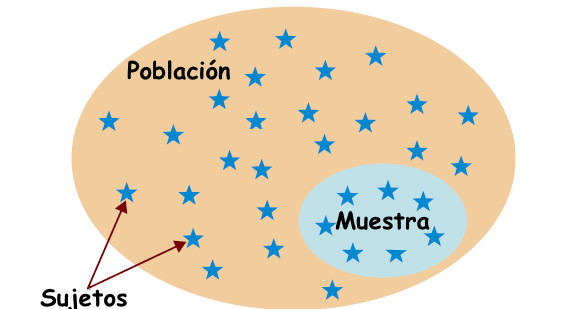
\includegraphics[width=0.6\linewidth]{INREMDN_files/figure-html/samplingcast} 

}

\caption{Población *versus* muestra}\label{fig:samplingcast}
\end{figure}

\begin{example}
\protect\hypertarget{exm:caldo}{}\label{exm:caldo}Si queremos saber si un guiso nos ha quedado soso, no nos lo comemos todo, porque entonces nos quedaríamos sin guiso y ya no valdría la pena saber si está soso o no. Lo que hacemos es probar solo una cucharada. El guiso es la población, la cucharada la muestra. A partir del sabor de la cucharada, ``inferimos'' cómo nos ha quedado el guiso.
\end{example}

En general, una \textbf{población} es simplemente un conjunto de individuos u objetos (genéricamente, de \textbf{sujetos}) sobre los que queremos conocer alguna información. Esta población puede estar perfectamente definida en un lugar y tiempo: por ejemplo, los empadronados en Mallorca a día de hoy. Pero normalmente su definición será difusa. Si, por ejemplo, queremos estimar algo sobre ``los españoles diabéticos mayores de 65 años'', ¿de quiénes estamos hablando exactamente? ¿De los que están vivos justo ahora? ¿De todos los que ha habido en España desde su fundación? ¿Incluimos los que aún no han nacido? ¿Qué hacemos con los que son diabéticos pero no han sido diagnosticados, ni lo serán nunca?

Tranquilos, no nos vamos a romper mucho la cabeza con esto. Pero al menos tenéis que ser conscientes de que una población puede contener sujetos que en realidad no existen ni hayan existido ni vayan a existir, sino simplemente que ``podrían existir''. Y en medicina especialmente, cuando queremos estimar si un tratamiento será efectivo para tratar una cierta enfermedad\ldots{} incluyendo los casos que aún no han contraído la enfermedad. Hablaremos entonces de una población \textbf{virtual} (en otros lugares la califican de población \textbf{metafórica}).

Por ejemplo, cuando decimos que

\begin{quote}
``La probabilidad de que salga Cara al lanzar una moneda equilibrada es 1/2'',
\end{quote}

lo que significa es que

\begin{quote}
``Si tomamos la población formada por todos los posibles lanzamientos de todas las posibles monedas equilibradas, en la mitad de estos lanzamientos el resultado es Cara.''
\end{quote}

Los sujetos de esta población son todos los ``posibles'' lanzamientos de monedas equilibradas, los que se han realizado a lo largo de la historia, los que se realizarán en el futuro, y los que se podrían haber realizado o se podrían realizar en el futuro pero en realidad no han tenido lugar ni se efectuarán.

Otro ejemplo. Imaginad que comparamos las notas que (vosotros, estudiantes de primer curso del grado de Medicina de la UIB de este año académico) sacáis en dos cuestionarios diferentes sobre un mismo tema, uno sobre conceptos y el otro de cálculos, y que en el primero obtenéis una nota media mucho mayor que en el segundo. Usamos este dato para inferir que los estudiantes de primer curso de Medicina sacan de media mejor nota en tests de conceptos que en tests calculísticos. ¿Quiénes son estos ``estudiantes de primer curso de Medicina''? ¿Sobre qué población ``inferimos'' información a partir de este resultado?

No sobre solo vosotros para estos dos tests concretos, ya que entonces no estaríamos infiriendo nada, simplemente calificaríamos, constataríamos que una nota media ha sido más alta que la otra, y pararíamos aquí.

La población a la que podríamos querer generalizar los resultados podríais ser vosotros, pero para ``siempre que hicierais'' tests calculísticos y de conceptos. O podrían ser las personas matriculadas en alguna asignatura de primer curso del grado de Medicina de España en este curso académico, que es una población bien definida. O podría ser la población virtual de ``estudiantes de primer curso de Medicina'', pasados, presentes y futuros y con una noción imprecisa de lo que entendemos por ``estudiante de primer curso''.

Hasta ahora hemos hablado de la población, a menudo virtual, sobre la que queremos obtener información. Está será nuestra \textbf{población objetivo}, que hay que distinguir de la \textbf{muestra}:

\begin{itemize}
\item
  \textbf{Población objetivo}: un conjunto de sujetos con una o varias características sobre las que deseamos obtener información.
\item
  \textbf{Muestra}: el grupo de unidades de observación en las que medimos las características de interés.
\end{itemize}

Normalmente, la muestra es un subconjunto de la población objetivo, pero ya hemos visto en la sección anterior que esto no siempre es así: pensad en los estudios ecológicos.

\begin{example}
\protect\hypertarget{exm:unnamed-chunk-57}{}\label{exm:unnamed-chunk-57}Una serie de 10 lanzamientos de una moneda equilibrada concreta es una muestra de la población de ``los posibles lanzamientos de monedas equilibradas''.
\end{example}

\begin{example}
\protect\hypertarget{exm:unnamed-chunk-58}{}\label{exm:unnamed-chunk-58}

¿Y vosotros qué sois: una población o una muestra? Pues depende:

\begin{itemize}
\item
  Sois una población cuando lo que nos interesa es saber algo sobre \textbf{vosotros} y solo sobre vosotros.
\item
  Sois una muestra si a partir de información sobre vosotros miramos de inferir información sobre \textbf{un grupo más grande de sujetos}:

  \begin{itemize}
  \tightlist
  \item
    Sobre los estudiantes de primer curso de Medicina en España
  \item
    Sobre los estudiantes de la UIB de este curso
  \item
    Sobre los jóvenes europeos
  \item
    Sobre los mamíferos bípedos
  \item
    Sobre \ldots{}
  \end{itemize}
\end{itemize}

\end{example}

\begin{rmdrecordau}
Procurad tener siempre presente que, por mucho cuidado que pongamos en obtener una muestra de una población, nunca será nada más que una aproximación imperfecta de esta.
\end{rmdrecordau}

Si podemos medir todos los individuos de la población objetivo, no nos hace falta usar estadística inferencial para intentar adivinar lo que queremos saber sobre la población: lo medimos sobre todo el mundo y ya está. Pero lo más normal es que no podamos medir todos los individuos de la población.

\begin{itemize}
\item
  La población puede ser demasiado grande. Por ejemplo, si queremos calcular la altura media de los europeos que hoy tienen 18 años, es prácticamente imposible medirlos todos.
\item
  Como ya hemos comentado, la población puede ser \textbf{virtual} en el sentido de que puede contener miembros que en este momento ni existan, o que no podamos saber si pertenecen o no a dicha población.
\item
  Puede ser que para obtener la información de un sujeto lo tengamos que sacrificar (por ejemplo, si la información solo se puede recoger con una autopsia). En este caso, para medir toda la población la tendríamos que exterminar.
\item
  Puede ser simplemente que sea difícil acceder a toda la población: por ejemplo, los estudiantes de la UIB son relativamente pocos, unos 12000, pero sería complicado conseguir mediros a todos.
\end{itemize}

A la hora de determinar la validez de un estudio, es muy importante comparar la población objetivo con la:

\begin{itemize}
\tightlist
\item
  \textbf{Población muestreada}: el conjunto de sujetos (\textbf{unidades de observación}) del que se extrae la muestra.
\end{itemize}

\begin{figure}

{\centering 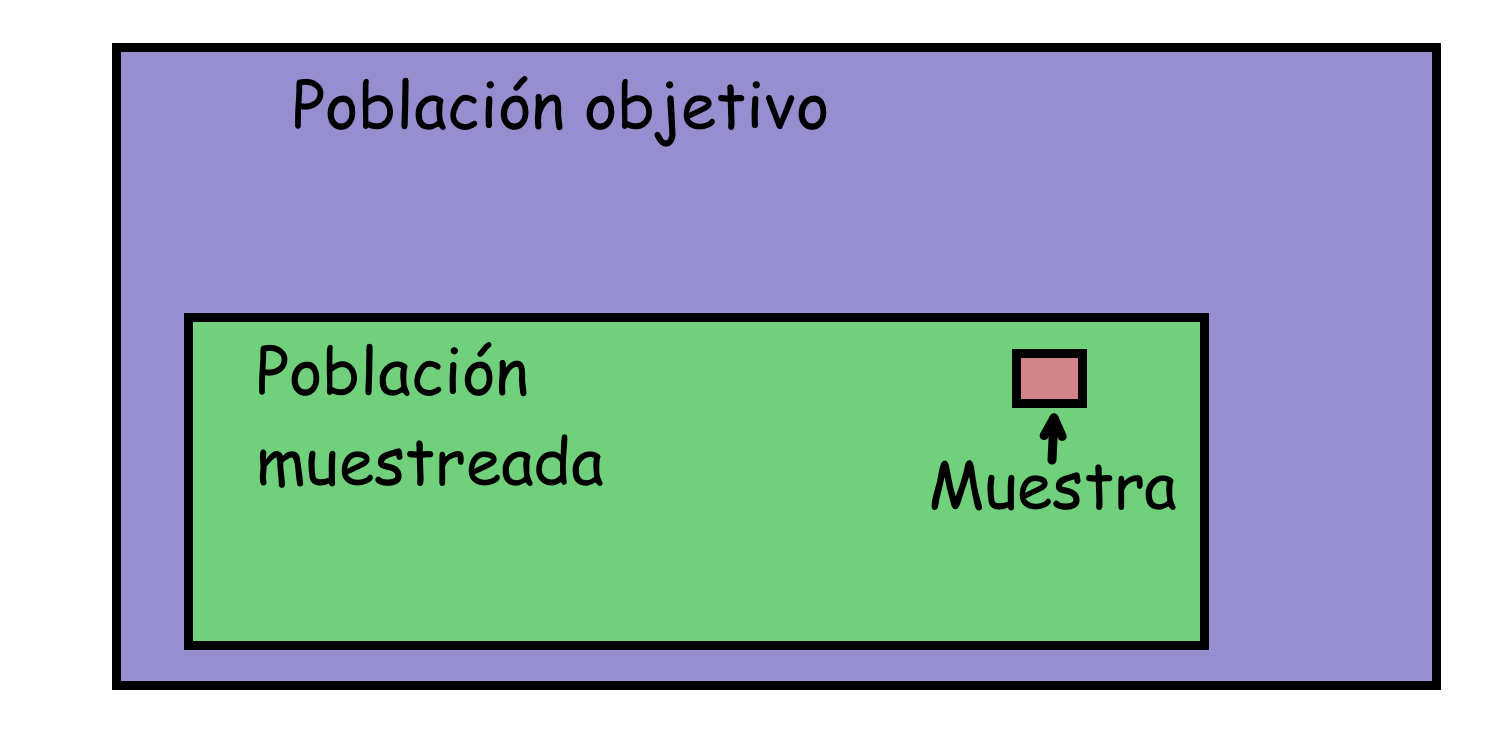
\includegraphics[width=0.8\linewidth]{INREMDN_files/figure-html/muestra} 

}

\caption{Población objetivo, población muestrada y muestra.}\label{fig:muestra}
\end{figure}

En la mayoría de las ocasiones, la población muestreada será un subconjunto de la población objetivo definido por una serie de restricciones, pero puede no serlo: pensad, por ejemplo, en los estudios ecológicos, donde la población objetivo son individuos y la población muestreada son grupos de individuos.

\begin{example}
\protect\hypertarget{exm:tuberculosisrusia}{}\label{exm:tuberculosisrusia}Dad un vistazo al artículo \href{https://www.bmj.com/content/332/7533/85.short}{``Risk factors for pulmonary tuberculosis in Russia: case-control study''}
(R. Coker \emph{et al}, \emph{British Medical Journal} 332 (2006), pp.~85-87). Su objetivo es ``Determinar los factores de riesgo para la tuberculosis pulmonar en Rusia''. Por lo tanto:
\end{example}

\begin{itemize}
\tightlist
\item
  La \textbf{población objetivo} es ``toda la población de Rusia'', sea lo que sea lo que signifique esto.
\end{itemize}

Ahora bien, la muestra se tomó solo entre los adultos de la ciudad de \href{https://es.wikipedia.org/wiki/Samara}{Samara} y durante 2003. Por lo tanto:

\begin{itemize}
\tightlist
\item
  La \textbf{población muestreada} fueron los adultos que vivían en Samara en 2003.
\end{itemize}

Finalmente, leemos que los casos fueron todos los adultos de esta ciudad diagnosticados de tuberculosis pulmonar a los que se administró un DOTS (Tratamiento Acortado Directamente Observado), en total 334. Como controles se tomó al azar el mismo número de personas entre la población adulta de la ciudad sin historial de tuberculosis.

\begin{itemize}
\tightlist
\item
  La \textbf{muestra} fueron estas 668 personas.
\end{itemize}

\begin{example}
\protect\hypertarget{exm:Hola}{}\label{exm:Hola}Para conocer la opinión de sus lectores sobre la familia real española, una conocida revista del corazón propuso una encuesta en línea en su web y analizó las respuestas. En este \textbf{estudio transversal}:
\end{example}

\begin{itemize}
\tightlist
\item
  La \textbf{población objetivo} es la formada por ``los lectores de esta revista''.
\item
  La \textbf{población muestreada} es la formada por los lectores de esta revista con acceso a Internet el año en que se realizó la encuesta.
\item
  La \textbf{muestra} es el grupo de personas concretas que voluntariamente respondieron la encuesta.
\end{itemize}

En el Ejemplo \ref{exm:tuberculosisrusia}, puede que la población muestreada no fuera representativa de \textbf{toda} Rusia. Los habitantes de Samara, una de las ciudades más pobladas de Rusia, a unos 1500 km al sudeste de Moscú, ¿son representativos de los habitantes de una aldea perdida en mitad de la nada siberiana? Pues no lo sabemos, pero creemos que no. Además, la muestra de casos tampoco representa el colectivo de tuberculosos de Samara, puesto que solo se reclutaron los que reunían las condiciones para un tratamiento concreto (los tuberculosos con frotis bucal negativo a veces no se incluyen en un programa DOTS).

En el Ejemplo \ref{exm:Hola} está más claro que la población muestreada no es representativa de la población objetivo: seguramente excluye, por ejemplo, los lectores ancianos o los de zonas rurales con acceso difícil a Internet. Además, la muestra es aún más restrictiva, ya que los participantes fueron voluntarios, y sus características pueden ser diferentes de las de los lectores que prefirieron no opinar sobre este tema (nunca se sabe si el CNI vigila\ldots) o de las de los lectores que nunca responden encuestas.

Si la población muestreada no es representativa de la población objetivo, los resultados del estudio no tienen por qué poderse generalizar a esta última: diremos entonces que se ha dado un \textbf{sesgo de falta de representatividad}. Hablaremos sobre sesgos en la Sección \ref{sec:sesgos}.

\begin{example}
\protect\hypertarget{exm:unnamed-chunk-60}{}\label{exm:unnamed-chunk-60}Al escogeros a vosotros como una muestra de la población de estudiantes de primer curso de Medicina, podríamos entender como población muestreada, por ejemplo, la de ``los estudiantes que este año académico cursan alguna asignatura de primer curso de Medicina en una universidad española''. Pero seguramente esta población difiera en algunos aspectos de los estudiantes de primer curso de Medicina de hace unos años, antes de la pandemia.
\end{example}

Un estudio médico toma información sobre una muestra de individuos y la generaliza a una población objetivo. Si nos ha interesado leerlo, seguramente será porque su población objetivo contiene, o al menos está relacionada con, la población que nos interesa a nosotros. Pero la muestra habrá sido tomada de una población muestreada que no tiene por qué coincidir con nuestra población de interés. Es muy importante poder decidir entonces si las conclusiones a las que se llega en el estudio se pueden aplicar o no a nuestra población. No es el objetivo de este curso el que podáis tomar esta decisión, ya que la respuesta no va de estadística sino de la experiencia médica que aún os falta. Pero sí que al menos seáis conscientes de que un resultado estimado para una población puede no ser extrapolable a otra población.

\begin{example}
\protect\hypertarget{exm:unnamed-chunk-61}{}\label{exm:unnamed-chunk-61}En el estudio \href{https://link.springer.com/article/10.1186/s40560-020-00466-z}{``D-dimer as a biomarker for disease severity and mortality in COVID-19 patients: a case control study''}(Y. Yao \emph{et al}, \emph{Journal of Intensive Care} 8:49 (2020)) se compararon diversas características clínicas, analíticas y radiológicas entre los pacientes que fallecieron (17 en total) y los que no fallecieron (231) en un grupo de enfermos de COVID-19 tratados en el hospital Renmin de la Universidad de Wuhan. Su objetivo era determinar qué características aumentaban el riesgo de defunción entre los enfermos de COVID-19.

Se encontró una asociación estadísticamente significativa entre tener un nivel de dímero D en sangre muy alto, superior a 2 mg/l, y un aumento en la letalidad de la COVID-19. Querríamos decidir si esta asociación también es válida para nuestros pacientes.
\end{example}

¿Cuál es el problema? Pues que la población objetivo del estudio es la de todos los enfermos de COVID-19, pero según el artículo la población muestreada fue la de ``pacientes con al menos dos síntomas de COVID-19 y PCR positiva tratados en ese hospital concreto de Wuhan''. Así que de entrada, los infectados con un solo síntoma quedan excluidos, por muy grave que sea ese síntoma. Además, habría que valorar si la población asignada a ese hospital se parece o no a la balear. Por ejemplo, la tasa de letalidad de la COVID-19 entre el grupo de pacientes examinados fue del 6.85\%, mientras que en las Baleares en esa misma época era de alrededor del 2.4\%, aunque este dato refiere al total de infectados, incluyendo los asintomáticos. También habría que tener en cuenta las posibles diferencias en los niveles ``normales'' de dímero D en sangre entre las personas de origen asiático y las de origen mediterráneo. Y habría que valorar si la asociación observada se debe a algún confundidor. Por ejemplo, la edad media de los sujetos de la muestra con niveles elevados de dímero D era más alta que la de los que tenían un nivel normal, y la COVID-19 es más letal entre los ancianos. ¿Será la edad un factor de confusión en este estudio?

\begin{rmdexercici}
En el artículo \href{https://bmcresnotes.biomedcentral.com/articles/10.1186/1756-0500-5-682}{``Tuberculosis treatment survival of HIV positive TB patients on directly observed treatment short-course in Southern Ethiopia: A retrospective cohort study''} (D. Shaweno, \emph{BMC Research Notes} 5:682 (2012)) se quiso estudiar si la infección por VIH afecta la supervivencia a corto plazo de pacientes con tuberculosis (TB). Para ello, se consideraron todos los pacientes que habían participado en un estudio previo: se trataba de pacientes diagnosticados de TB durante el periodo 2006-2010 a los que se prescribió un tratamiento concreto de quimioterapia de 8 meses de duración y que además pasaron un test de VIH en el momento del diagnóstico positivo de TB. De este grupo de pacientes, se escogieron al azar un subgrupo de 370 VIH-positivos y otro de 370 VIH-negativos, y se anotó el número de pacientes de cada subgrupo que fallecieron antes de finalizar el tratamiento de 8 meses. La conclusión fue que la tasa de mortalidad entre los paciente de TB VIH-positivos es mayor que entre los que son VIH-negativos.

\emph{(a)} ¿De qué tipo de estudio se trata?

\emph{(b)} ¿Cuáles son la población objetivo, la población muestreada y la muestra?

\emph{(c)} ¿Creéis que la población muestreada es representativa de la población objetivo?
\end{rmdexercici}

\hypertarget{sec:muestreo}{%
\section{Tipos básicos de muestreo}\label{sec:muestreo}}

En un estudio estadístico inferencial, se toma una \textbf{muestra} de individuos de una \textbf{población} y se estiman algunas características de la población a partir de las de la muestra. Para que esto tenga sentido, es necesario que la muestra sea razonablemente \textbf{representativa} de la población. Pero, claro, sin conocer las características de la población, no podemos saber si una muestra es representativa o no.

Para salir de este \emph{impasse}, la solución comúnmente aceptada es tomar una muestra \textbf{aleatoria}, es decir, escogiendo sus sujetos de alguna manera al azar. Al hacerlo así:

\begin{itemize}
\tightlist
\item
  Se evitan preferencias en la elección, por lo que es más probable que la muestra sea representativa de la población. Naturalmente, esto no está garantizado: por pura mala suerte nos puede salir una muestra súper rara, es lo que tiene el azar.
  Pero al menos hemos hecho ``lo que todo el mundo considera que es lo que hay que hacer'' para intentar que sea representativa.
\end{itemize}

\begin{figure}

{\centering 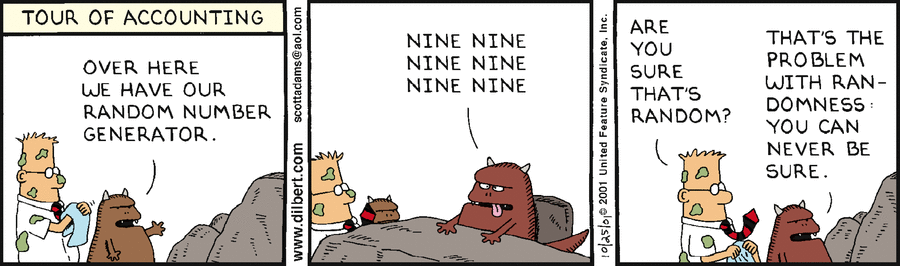
\includegraphics[width=0.8\linewidth]{INREMDN_files/figure-html/randomgen} 

}

\caption{¿Estás seguro de que la muestra es aleatoria? (http://dilbert.com/strip/2001-10-25)}\label{fig:unnamed-chunk-63}
\end{figure}

\begin{itemize}
\tightlist
\item
  Se pueden usar técnicas estadísticas que permiten acotar errores en la estimación y su probabilidad; por ejemplo, que permite calcular la probabilidad de que nuestra muestra sea súper rara en algún sentido concreto.
\end{itemize}

\begin{example}
\protect\hypertarget{exm:unnamed-chunk-64}{}\label{exm:unnamed-chunk-64}Para probar el guiso, antes de tomar una cucharada lo removemos bien. De este modo esperamos que las moléculas del caldo se organicen de manera aleatoria dentro de la olla y que la cucharada que tomemos sea representativa del guiso.
\end{example}

Existen muchos métodos de \textbf{muestreo}. A continuación describimos algunos de forma breve.

\hypertarget{sec:mas}{%
\subsection{Muestreo aleatorio con y sin reposición}\label{sec:mas}}

El \textbf{muestreo aleatorio} consiste en seleccionar una muestra de la población de manera que todas las muestras del mismo tamaño sean \textbf{equiprobables}; es decir, que si fijamos el número de individuos de la muestra, cualquier conjunto de ese número de individuos tenga la misma probabilidad de ser seleccionado.

Hay que distinguir entre dos tipos de muestreo aleatorio: \textbf{con} y \textbf{sin reposición}, según permitamos o no que se repitan sujetos en la muestra. Para ilustrarlos, supongamos que disponemos de una urna con 100 bolas numeradas del 1 al 100, de la que queremos extraer una muestra de 15 bolas. La Figura \ref{fig:base} representa dicha urna.

\begin{figure}

{\centering 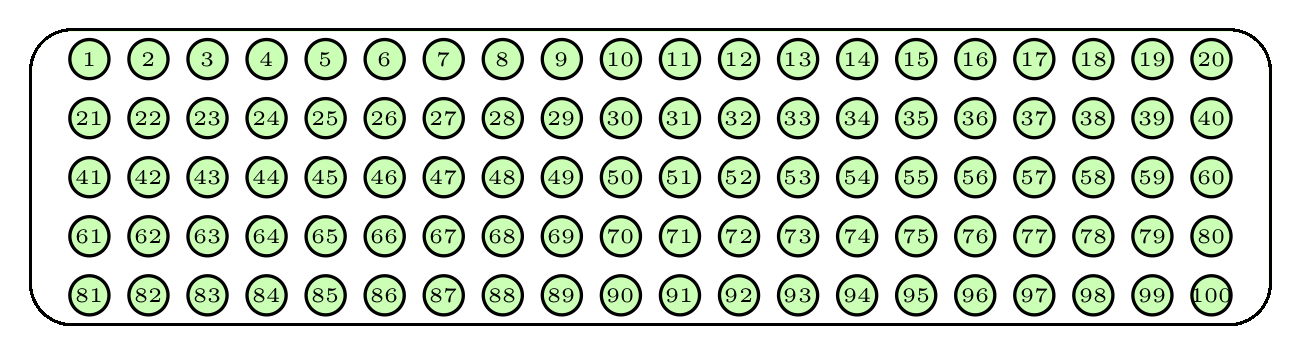
\includegraphics[width=0.8\linewidth]{INREMDN_files/figure-html/basev} 

}

\caption{Una urna de 100 bolas.}\label{fig:base}
\end{figure}

Una manera de hacerlo sería repetir 15 veces el proceso de sacar una bola de la urna, anotar su número y devolverla a la urna. El tipo de muestra obtenida de esta manera recibe el nombre de \textbf{muestra aleatoria con reposición}, o \textbf{muestra aleatoria simple}. Observad que con este procedimiento una misma bola puede aparecer varias veces en una muestra, y que todos los subconjuntos de 15 bolas ``con posibles repeticiones'' tienen la misma probabilidad de obtenerse. Un posible resultado serían las bolas azules de la Figura \ref{fig:simple}; la bola azul más oscuro ha sido escogida dos veces en la muestra.

\begin{figure}

{\centering 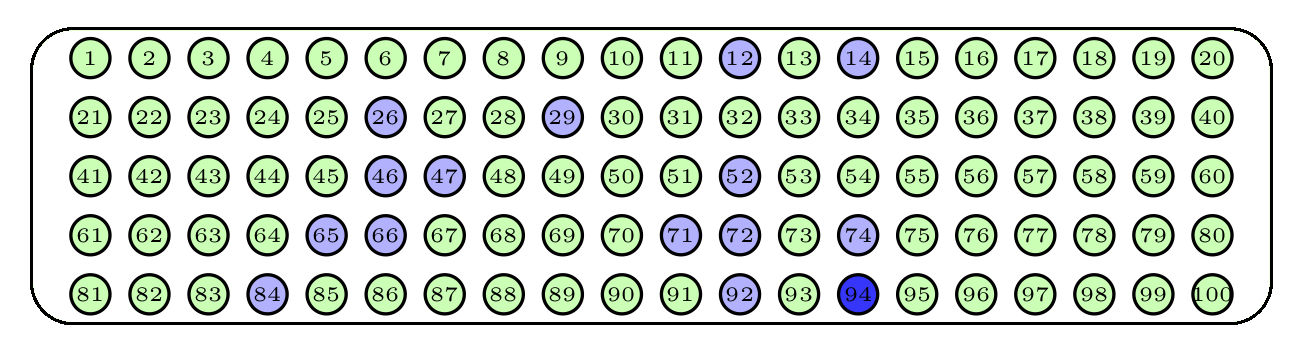
\includegraphics[width=0.8\linewidth]{INREMDN_files/figure-html/simplev} 

}

\caption{Una muestra aleatoria simple.}\label{fig:simple}
\end{figure}

Otra manera de extraer la muestra sería repetir 15 veces el proceso de sacar una bola de la urna pero ahora sin devolverla. Esto es equivalente a extraer de golpe 15 bolas de la urna. Estas muestras no tienen bolas repetidas, y cualquier selección de 15 bolas diferentes tiene la misma probabilidad de ser la obtenida. En este caso se habla de una \textbf{muestra aleatoria sin reposición}. Un posible resultado serían las bolas azules de la Figura \ref{fig:sinrep}.

\begin{figure}

{\centering 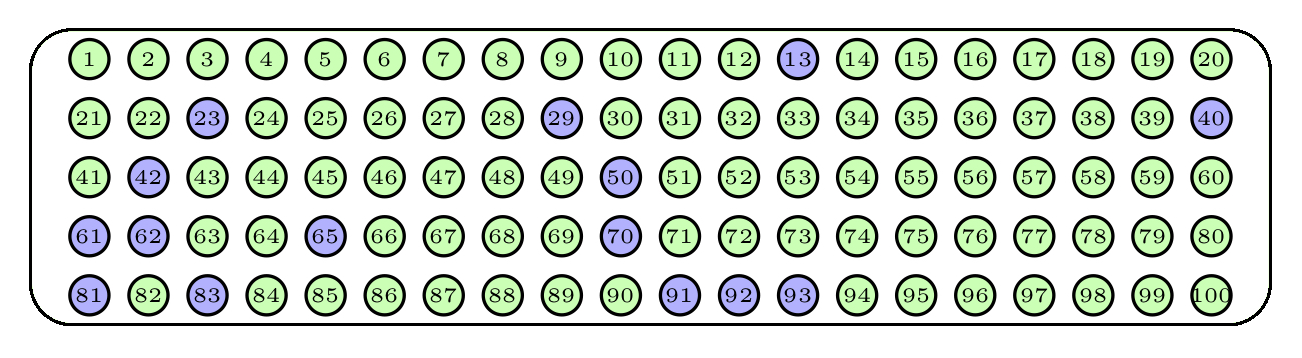
\includegraphics[width=0.8\linewidth]{INREMDN_files/figure-html/sinrepv} 

}

\caption{Una muestra aleatoria sin reposición.}\label{fig:sinrep}
\end{figure}

Cuando \textbf{el tamaño de la población es muy grande en relación al de la muestra}, como suele suceder en medicina, la probabilidad de que haya repeticiones en una muestra aleatoria simple es muy pequeña. Por ejemplo:

\begin{itemize}
\item
  Si escogemos 100 individuos de las Baleares (que tiene alrededor de 1,150,000 habitantes) al azar permitiendo repeticiones, la probabilidad de que se escoja más de una vez algún individuo es de 0.004: de media, solo en 1 de cada 250 muestras de 100 individuos de las Baleares elegidos al azar permitiendo repeticiones nos saldría alguien repetido.
\item
  Si escogemos 100 estudiantes de la UIB (que tiene alrededor de 12000 estudiantes) al azar permitiendo repeticiones, la probabilidad de que se escoja más de una vez algún individuo es de 0.339: de media, en algo más de 1 de cada 3 muestras de 100 estudiantes de la UIB elegidos al azar permitiendo repeticiones habría alguien repetido.

  En cambio, si escogemos \textbf{10} estudiantes de la UIB al azar permitiendo repeticiones, la probabilidad de que se escoja más de una vez algún individuo ya es de 0.004.
\end{itemize}

\begin{rmdnote}
Ya daremos el detalle de cómo se calculan todas estas probabilidades en el tema siguiente.
\end{rmdnote}

Esto nos permite considerar que, cuando la población es mucho más grande que la muestra, los muestreos aleatorios con y sin reposición son \textbf{equivalentes} en el sentido siguiente: puesto que si la población es muy, muy grande, una muestra aleatoria con reposición tendría casi seguro todos los elementos diferentes, podemos tomar directamente la muestra sin reposición y aceptar que permitíamos repeticiones, pero que no se han dado y que por tanto la muestra es simple.

\begin{itemize}
\item
  Una muestra aleatoria de 100 individuos diferentes de las Baleares, o de 10 estudiantes diferentes de la UIB, puede pasar perfectamente por una muestra simple, porque aunque permitiéramos repeticiones, sería muy raro que las hubiera.
\item
  Pero en cambio ya es difícil de creer que una muestra aleatoria de 100 estudiantes diferentes de la UIB haya sido tomada permitiendo repeticiones, porque de media en una de cada tres muestras tomadas permitiendo repeticiones nos saldría alguna repetición.
\end{itemize}

El muestreo aleatorio simple es el \emph{estándard de excelencia} entre los métodos de muestreo, y la mayoría de los resultados que explicaremos en este curso presuponen que la muestra ha sido tomada aleatoria con reposición. Pero casi nunca es factible hacerlo. El motivo es que para poder tomar una muestra aleatoria de una población en el sentido de este apartado, con o sin reposición, es necesario disponer de una lista completa de todos sus individuos para poder sortear a quién vamos a seleccionar. Esto no siempre es posible. ¿Alguien tiene la lista completa de, pongamos, todos los diabéticos de España? ¿Que incluya los que no saben que lo son? Por lo tanto, en la vida real no siempre podemos tomar muestras aleatorias en este sentido.

\hypertarget{muestras-aleatorias-con-r}{%
\paragraph*{Muestras aleatorias con R}\label{muestras-aleatorias-con-r}}
\addcontentsline{toc}{paragraph}{Muestras aleatorias con R}

Cualquier paquete estadístico que se precie permite obtener muestras aleatorias de conjuntos. Con R, la función básica es

\begin{Shaded}
\begin{Highlighting}[]
\FunctionTok{sample}\NormalTok{(x, n, }\AttributeTok{replace=}\NormalTok{...)}
\end{Highlighting}
\end{Shaded}

donde:

\begin{itemize}
\item
  \texttt{x} es un vector que contiene toda la población o un número natural \(x\); en este último caso, R entiende que representa el vector 1,2,\ldots,\(x\);
\item
  \texttt{n} es el tamaño de la muestra que deseamos extraer;
\item
  el parámetro \texttt{replace} puede igualarse a \texttt{TRUE}, y será una muestra aleatoria con reposición, es decir, simple, o a \texttt{FALSE}, y será una muestra aleatoria sin reposición. Si no se especifica este parámetro, R entiende que ha de tomar la muestra sin reposición.
\end{itemize}

Así, por ejemplo, para obtener una muestra aleatoria simple de 15 números elegidos entre 1 y 100, podemos entrar:

\begin{Shaded}
\begin{Highlighting}[]
\FunctionTok{sample}\NormalTok{(}\DecValTok{100}\NormalTok{,}\DecValTok{15}\NormalTok{,}\AttributeTok{replace=}\ConstantTok{TRUE}\NormalTok{)}
\end{Highlighting}
\end{Shaded}

\begin{verbatim}
##  [1] 100  51  78  55  75  68   6  63  78  92  14   7  93  55  86
\end{verbatim}

Naturalmente, cada ejecución de \texttt{sample} con los mismos parámetros puede dar (y seguramente dé) lugar a muestras diferentes, y todas ellas tienen la misma probabilidad de aparecer:

\begin{Shaded}
\begin{Highlighting}[]
\FunctionTok{sample}\NormalTok{(}\DecValTok{100}\NormalTok{,}\DecValTok{15}\NormalTok{,}\AttributeTok{replace=}\ConstantTok{TRUE}\NormalTok{)}
\end{Highlighting}
\end{Shaded}

\begin{verbatim}
##  [1] 69  1 51 32 65 98 29 12 79 60 44 70 63 22 69
\end{verbatim}

\begin{Shaded}
\begin{Highlighting}[]
\FunctionTok{sample}\NormalTok{(}\DecValTok{100}\NormalTok{,}\DecValTok{15}\NormalTok{,}\AttributeTok{replace=}\ConstantTok{TRUE}\NormalTok{)}
\end{Highlighting}
\end{Shaded}

\begin{verbatim}
##  [1] 11 92 20 62 72  3 68 29 66 34 72 39 97 31 83
\end{verbatim}

\begin{Shaded}
\begin{Highlighting}[]
\FunctionTok{sample}\NormalTok{(}\DecValTok{100}\NormalTok{,}\DecValTok{15}\NormalTok{,}\AttributeTok{replace=}\ConstantTok{TRUE}\NormalTok{)}
\end{Highlighting}
\end{Shaded}

\begin{verbatim}
##  [1] 56  1 19 60 50 41  3 32 74 33 99 90 20 90 16
\end{verbatim}

\begin{example}
\protect\hypertarget{exm:unnamed-chunk-69}{}\label{exm:unnamed-chunk-69}En el marco de un estudio experimental, tenemos que asignar al azar 60 pacientes a dos tratamientos, de manera que cada paciente tenga un 50\% de probabilidades de caer en uno u otro grupo de tratamiento tratamiento. Si indicamos los dos tratamientos por 1 y 2 (por ejemplo, que 1 sea el tratamiento control y 2 el tratamiento nuevo), podemos numerar los sujetos de 1 a 60 y a continuación tomar una muestra aleatoria simple de tamaño 60 de valores 1 o 2 y a cada sujeto asignarle el tratamiento que le corresponda en esta muestra. Para ello, ejecutamos
\end{example}

\begin{Shaded}
\begin{Highlighting}[]
\FunctionTok{sample}\NormalTok{(}\DecValTok{2}\NormalTok{,}\DecValTok{60}\NormalTok{,}\AttributeTok{replace=}\ConstantTok{TRUE}\NormalTok{)}
\end{Highlighting}
\end{Shaded}

\begin{verbatim}
##  [1] 1 1 1 2 1 2 2 1 2 2 2 1 2 1 2 2 1 1 2 2 1 2 1 1 2 2 2 1 1 1 1 2 2 1 1 1 1 1
## [39] 1 2 1 2 1 2 2 2 2 1 1 2 1 2 2 1 2 2 2 1 1 1
\end{verbatim}

De esta manera se asignarían 31 pacientes al tratamiento 1 y 29 al tratamiento 2: los tres primeros al tratamiento 1, el cuarto al tratamiento 2, el quinto al tratamiento 1 etc.

Si hubiéramos querido forzar que cada grupo de tratamiento tuviera 30 pacientes, hubiéramos podido tomar una muestra aleatoria sin reposición de tamaño 30 de los 60 pacientes, asignar a sus miembros uno de los tratamientos y al resto el otro tratamiento. Así, podríamos asignar el tratamiento 1 a los pacientes

\begin{Shaded}
\begin{Highlighting}[]
\FunctionTok{sort}\NormalTok{(}\FunctionTok{sample}\NormalTok{(}\DecValTok{60}\NormalTok{,}\DecValTok{30}\NormalTok{,}\AttributeTok{replace=}\ConstantTok{FALSE}\NormalTok{))}
\end{Highlighting}
\end{Shaded}

\begin{verbatim}
##  [1]  1  2  3  4  5  8  9 13 16 17 19 20 22 26 29 32 34 36 38 39 40 42 45 46 50
## [26] 52 53 54 57 59
\end{verbatim}

(La función \texttt{sort}, como su nombre en inglés indica, sirve para ordenar vectores.)

\hypertarget{sec:sist}{%
\subsection{Muestreo sistemático}\label{sec:sist}}

Una manera muy sencilla de obtener una muestra de una población cuando disponemos de una lista ordenada de sus individuos y nos da pereza efectuar un sorteo es tomarlos a intervalos constantes: uno de cada cinco individuos, uno de cada diez\ldots{} Podemos añadir un componente aleatorio escogiendo al azar el primer individuo que elegimos, y a partir del cual empezamos a contar. A esta técnica se la llama \textbf{muestreo sistemático} o \textbf{a intervalos}, añadiendo el adjetivo \textbf{aleatorio} si además el primer sujeto se escoge de manera aleatoria.

Así, por ejemplo, si de una clase de 100 estudiantes quisiéramos escoger una muestra de 10, podríamos elegir un estudiante al azar, y a partir de él, por orden alfabético, elegir el décimo estudiante, el vigésimo, el trigésimo, etc.; si al llegar al final de la lista de clase no hubiéramos completado la muestra, volveríamos al principio de la misma.

La Figura \ref{fig:sist} describe una muestra aleatoria sistemática de 15 bolas de nuestra urna de 100 bolas: hemos empezado a escoger por la bola roja oscura, que ha sido elegida al azar, y a partir de ella hemos tomado las bolas a intervalos de 7, volviendo al principio cuando hemos llegado al final de la lista numerada.

\begin{figure}

{\centering 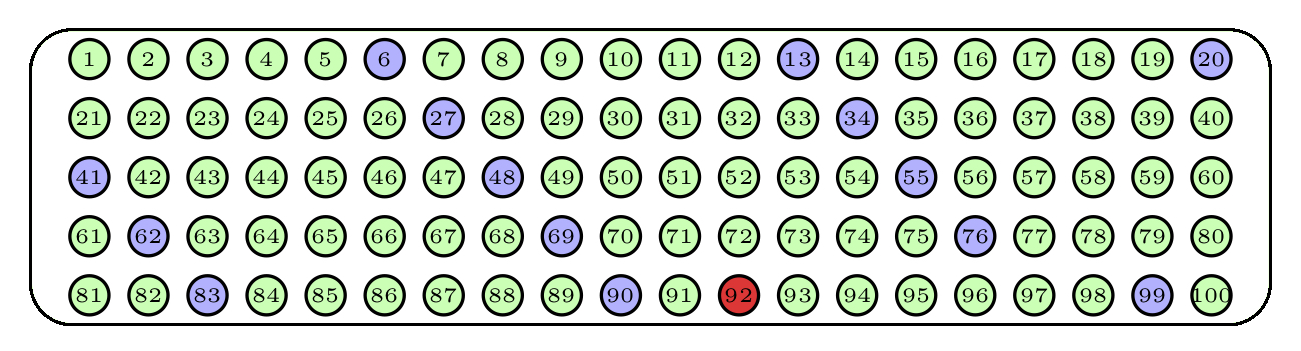
\includegraphics[width=0.8\linewidth]{INREMDN_files/figure-html/sistv} 

}

\caption{Una muestra aleatoria sistemática.}\label{fig:sist}
\end{figure}

Cuando no disponemos de una lista de toda la población pero sí que tenemos una manera de acceder de manera ordenada a sujetos de la misma (por ejemplo, enfermos que acuden a un hospital), podemos realizar un muestreo sistemático tomando los sujetos a intervalos constantes a medida que los encontramos y hasta completar el tamaño deseado de la muestra. Por ejemplo, para escoger una muestra de 10 pacientes que hayan acudido a Urgencias por traumatismos en la cabeza, podríamos escoger pacientes a intervalos regulares de entre los que acudieran a Urgencias por este motivo hasta llegar a los 10.

\begin{rmdnote}
Si la lista de la población está ordenada al azar, o si los sujetos que vamos tomando a intervalos regulares nos aparecen al azar, el resultado del muestreo sistemático es equivalente a una muestra aleatoria sin reposición.
\end{rmdnote}

\hypertarget{sec:estr}{%
\subsection{Muestreo aleatorio estratificado}\label{sec:estr}}

Este método de muestreo se utiliza cuando la población está clasificada en \textbf{estratos} que son de interés para la característica que se estudia. Estos estratos serán grupos de individuos definidos por un atributo concreto, de manera que individuos del mismo estrato tengan ese atributo igual (los estratos sean \textbf{homogéneos} internamente) y individuos de estratos diferentes tengan ese atributo diferente. Por ejemplo, la clasificación en estratos puede venir dada por los sexos, franjas de edad, provincias, casos y controles\ldots{} En este caso, se toma una muestra de un tamaño prefijado de cada estrato y se unen en una muestra global. Este proceso es llamado \textbf{muestreo estratificado}, \textbf{aleatorio} si la muestra de cada estrato es aleatoria (en el sentido de la Sección \ref{sec:mas}).

Por lo que refiere a los tamaños de las muestras de cada estrato, se suele optar por una de las estrategias siguientes:

\begin{itemize}
\item
  Imponer que la composición por estratos de la muestra global mantenga las proporciones de la población original, de manera que el tamaño de la muestra de cada estrato represente el mismo porcentaje del total de la muestra que el estrato correspondiente en la población completa.
\item
  Tomar las muestras de los diferentes estratos del mismo tamaño.
\item
  Tomar los tamaños de manera que los estratos que representen una fracción muy pequeña de la población (tan pequeña que no esperaríamos que tuvieran representación en una muestra aleatoria \textbf{transversal} de la población, es decir, tomada del total de la población sin tener en cuenta su composición en estratos) tengan una representación en la muestra mucho mayor que la que les tocaría.
\end{itemize}

\begin{figure}

{\centering 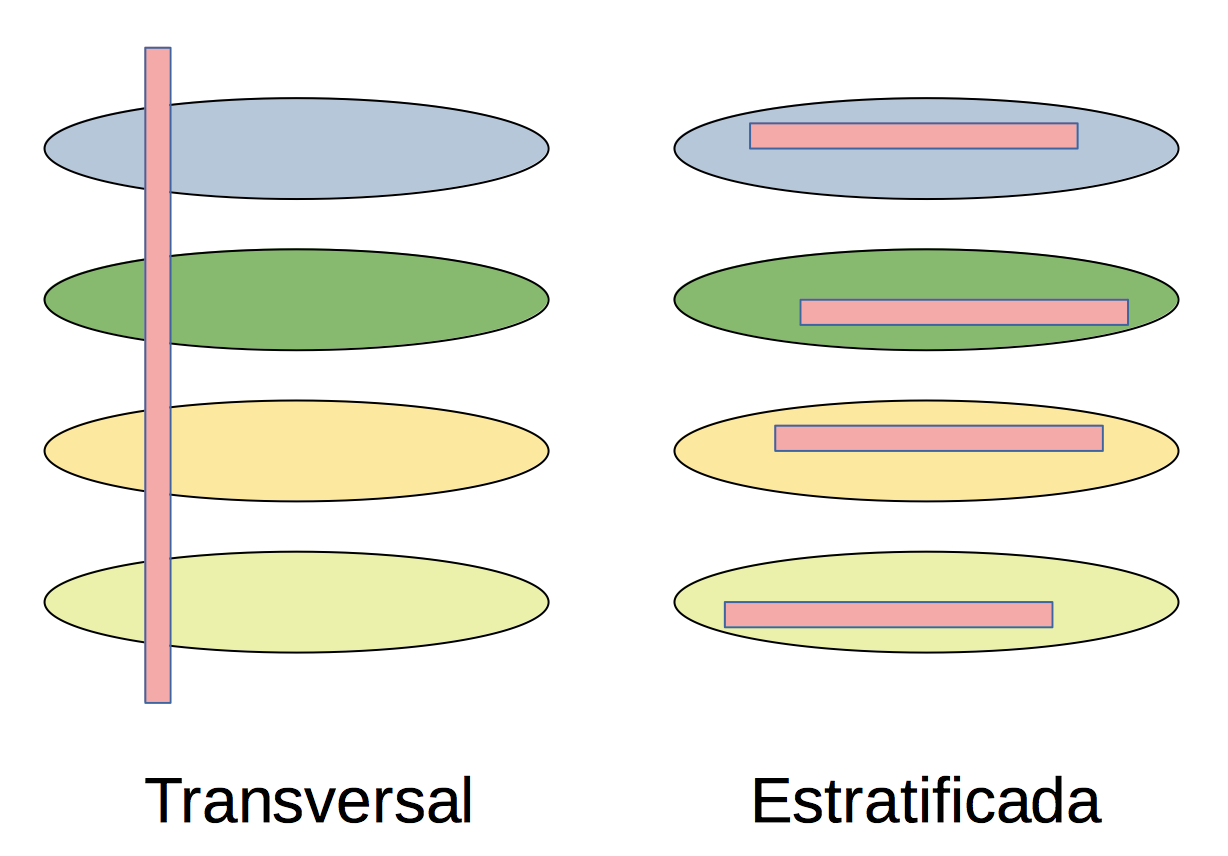
\includegraphics[width=0.6\linewidth]{INREMDN_files/figure-html/estratvstrans} 

}

\caption{Muestra transversal *versus* estratificada}\label{fig:unnamed-chunk-73}
\end{figure}

Por ejemplo, los estratos podrían ser grupos de edad y podríamos tomar la muestra de cada grupo de edad de tamaño proporcional a la fracción que representa dicho grupo de edad en la población total. O podrían ser los sexos y procuraríamos que nuestra muestra estuviera formada por un 50\% de hombres y un 50\% de mujeres. O, en las Islas Baleares, los estratos podrían ser las islas, y entonces podríamos imponer que el número de representantes de cada isla en la muestra fuera proporcional a su población relativa dentro del conjunto total de la Comunidad Autónoma, o podríamos tomar la misma cantidad de individuos de cada isla, independientemente de su población.

\begin{rmdnote}
Cuando en un estudio de casos y controles escogemos un grupo de casos y uno de controles de tamaños prefijados, o cuando en un estudio de cohorte escogemos un grupo de expuestos y uno de no expuestos de tamaños prefijados, se trata de una muestra estratificada, aunque no siempre será aleatoria.
\end{rmdnote}

Para continuar con nuestra urna de 100 bolas, supongamos que contiene 40 bolas de un color y 60 de otro color según muestra la Figura \ref{fig:estratprevi}.

\begin{figure}

{\centering 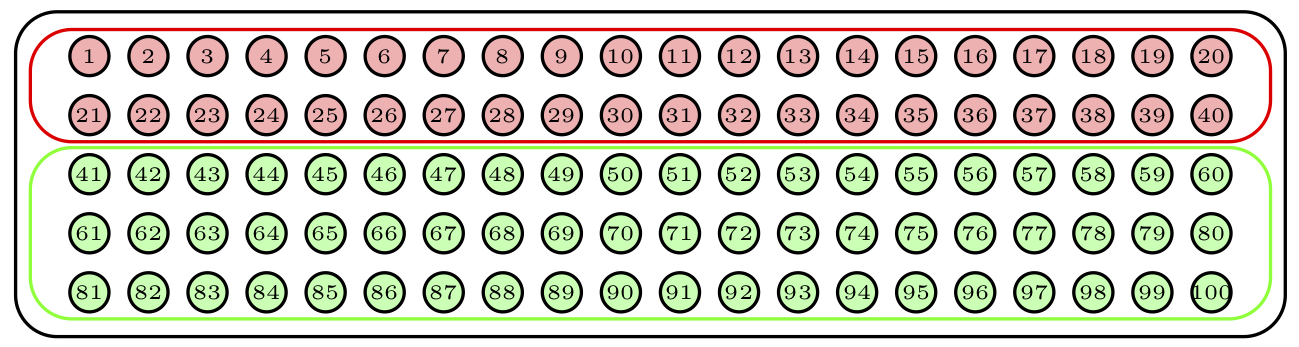
\includegraphics[width=0.8\linewidth]{INREMDN_files/figure-html/estratprevi} 

}

\caption{Nuestra urna ahora tiene dos  estratos.}\label{fig:estratprevi}
\end{figure}

Para tomar una muestra aleatoria estratificada de 15 bolas, considerando como estratos los dos colores e imponiendo que la muestra refleje la composición de la urna, tomaríamos una muestra aleatoria de 6 bolas del primer color y una muestra aleatoria de 9 bolas del segundo color. De esta manera, los porcentajes de colores en la muestra serían los mismos que en la urna. La Figura \ref{fig:estrat} describe una muestra obtenida de esta manera.

\begin{figure}

{\centering 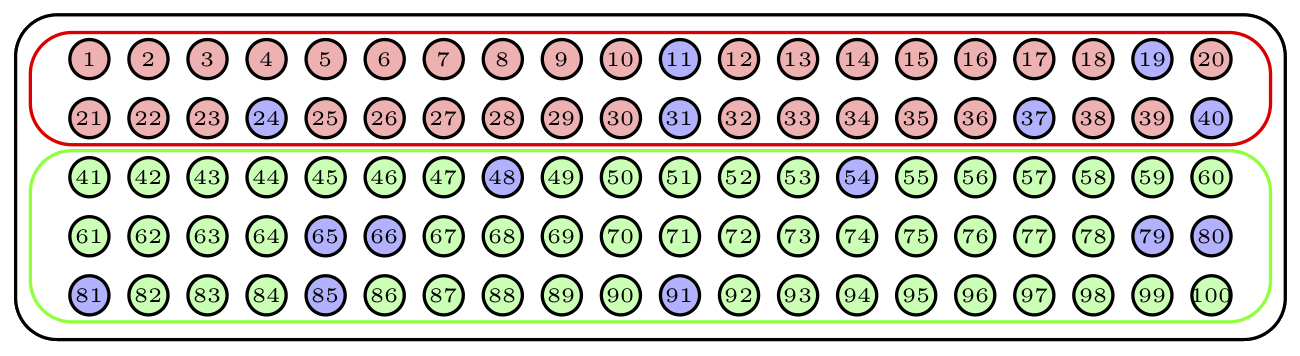
\includegraphics[width=0.8\linewidth]{INREMDN_files/figure-html/estrat} 

}

\caption{Una muestra aleatoria estratificada.}\label{fig:estrat}
\end{figure}

Para tomar una muestra aleatoria estratificada de 10 bolas, de nuevo considerando como estratos los dos colores pero ahora imponiendo que cada color aporte la misma cantidad de bolas a la muestra, tomaríamos una muestra aleatoria de 5 bolas del primer color y una muestra aleatoria de 5 bolas del segundo color. La Figura \ref{fig:estrathom} describe una muestra obtenida de esta manera.

\begin{figure}

{\centering 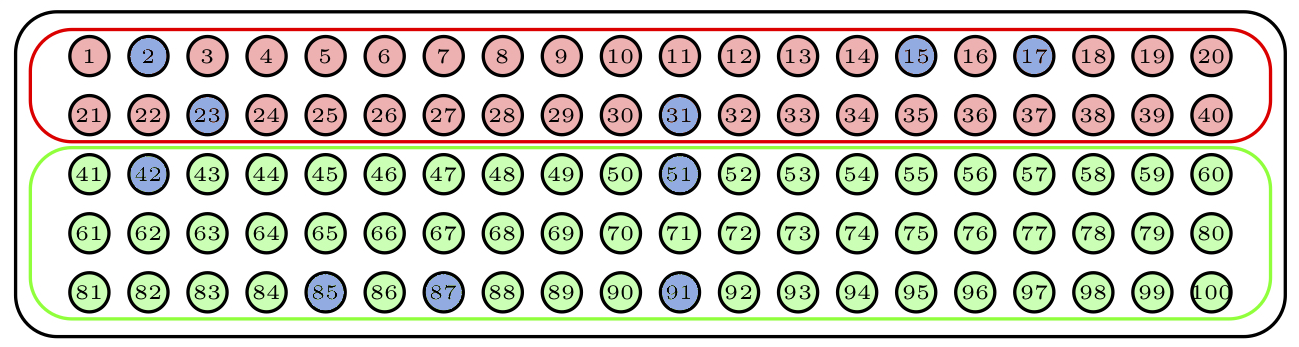
\includegraphics[width=0.8\linewidth]{INREMDN_files/figure-html/estrathom} 

}

\caption{Otra muestra aleatoria estratificada.}\label{fig:estrathom}
\end{figure}

La ventaja del muestreo aleatorio estratificado respecto del transversal es que, como el investigador escoge una muestra de cada estrato de la población del tamaño que considera adecuado:

\begin{itemize}
\item
  Permite estimar la información de interés para cada estrato por separado, como si se tratara de estudios independientes.
\item
  Permite estimar la información sobre subpoblaciones minoritarias que en una muestra aleatoria transversal aparecerían subrepresentadas.
\end{itemize}

En todo caso, el muestreo por estratos solo es necesario si esperamos que las características que queremos estudiar varíen según el estrato. Por ejemplo, si queremos tomar una muestra para estimar la altura media de los españoles adultos y no creemos que la altura de un español adulto dependa de su provincia de origen, no hay ninguna necesidad de esforzarse en tomar una muestra de cada provincia de manera que todas estén representadas adecuadamente en la muestra.

Observad que el muestreo aleatorio por estratos tiene el mismo inconveniente que el muestreo aleatorio de la Sección \ref{sec:mas}: es necesario disponer de una lista completa de los individuos de cada estrato para poder sortearlos.

\begin{rmdexercici}
Tenemos una población clasificada en dos estratos, A y B. La subpoblación A representa un 20\% de la población y la B el 80\% restante. Hemos tomado una muestra aleatoria estratificada formada por 100 sujetos de cada subpoblación. Hemos medido una cierta característica X de estos sujetos. La media de los valores de X de los sujetos A ha dado 5 y la media de los valores de X de los sujetos B ha dado 10.

\emph{(a)} ¿Qué vale la media de los valores de X de toda la muestra de 200 sujetos?

\emph{(b)} A partir de estos datos, ¿qué estimáis que vale la media de X en el total de la población?
\end{rmdexercici}

\hypertarget{sec:mcluster}{%
\subsection{Muestreo por conglomerados}\label{sec:mcluster}}

El proceso de obtener una muestra aleatoria en el sentido de las secciones anteriores puede ser caro o difícil en algunos casos, incluso aunque dispongamos de la lista completa de la población. Imaginad que quisiéramos estudiar la prevalencia y gravedad de la miopía entre los estudiantes de Primaria de las Baleares. Para ello tendríamos que seleccionar una muestra representativa de esta población de escolares. Seguramente, con algo de esfuerzo, podríamos disponer de su lista completa para este curso y por lo tanto podríamos tomar una muestra aleatoria, pero entonces acceder a las niñas y niños que la formasen seguramente significaría visitar muchos centros de primaria para entrevistar unos pocos alumnos de cada uno. Esto volvería el proceso lento y costoso. Y eso si consiguiéramos la lista global de alumnos.

Una alternativa posible sería, en vez de elegir una muestra aleatoria de todos los estudiantes de Primaria, escoger primero al azar unas pocas aulas de primaria de colegios de las Baleares, a las que llamamos en este contexto \textbf{conglomerados} o \textbf{clústers}, y formar entonces nuestra muestra con todos los alumnos de estas aulas. Estaréis de acuerdo en que es mucho más fácil disponer de la lista completa de estudiantes de unas pocas aulas que conseguir la lista completa de todos los estudiantes de la Comunidad, y mucho más cómodo ir a unos pocos colegios a entrevistar grupos enteros que ir a muchos colegios a entrevistar a unos pocos estudiantes de cada uno.

En un \textbf{muestreo aleatorio por conglomerados} o \textbf{clústers}, tenemos la población repartida en pequeños grupos, los clústers, y lo que hacemos es elegir al azar una muestra de clústers y tomar todos los individuos de los clústers elegidos.

Volviendo de nuevo a nuestra urna, supongamos que sus 100 bolas se agrupan en 20 conglomerados de 5 bolas cada uno según las franjas verticales de la Figura \ref{fig:clustprevi} (donde mantenemos la clasificación en dos colores para poder comparar el resultado del muestreo por conglomerados con el estratificado).

\begin{figure}

{\centering 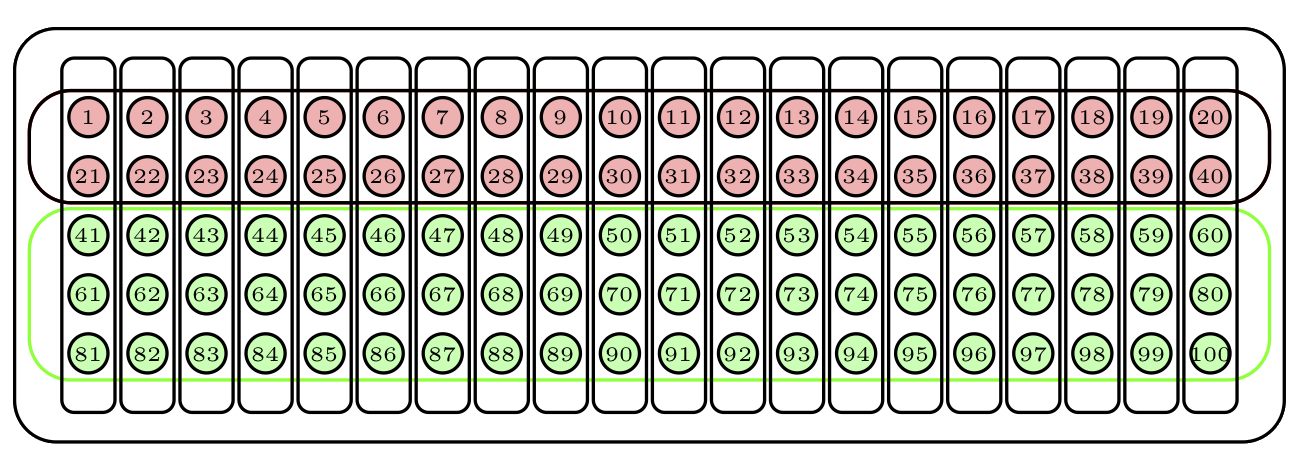
\includegraphics[width=0.8\linewidth]{INREMDN_files/figure-html/clusterprevi} 

}

\caption{Nuestra urna ahora tiene 2 estratos y 20 clústers.}\label{fig:clustprevi}
\end{figure}

Para obtener una muestra aleatoria por conglomerados de tamaño 15, escogeríamos al azar 3 conglomerados y la muestra estaría formada por todas sus bolas. La Figura \ref{fig:clust} describe una muestra obtenida de esta manera: los conglomerados escogidos están marcados en azul.

\begin{figure}

{\centering 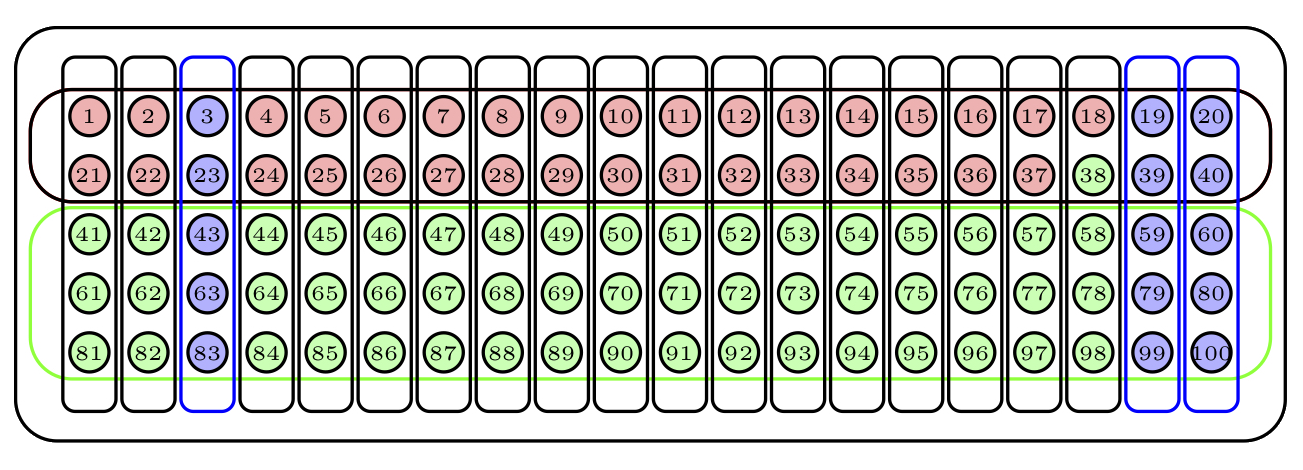
\includegraphics[width=0.8\linewidth]{INREMDN_files/figure-html/cluster} 

}

\caption{Una muestra aleatoria por conglomerados.}\label{fig:clust}
\end{figure}

A menudo una vez elegidos los clústers no se toman todos los sujetos de los mismos, sino una muestra aleatoria de cada uno. Esto ya sería un ejemplo de muestreo \textbf{polietápico} (Sección \ref{sec:poli}).

El muestreo por conglomerados se suele elegir por ser rápido de realizar, pero puede tener un inconveniente: puede que los sujetos de cada clúster tiendan a parecerse los unos a los otros, lo que puede sesgar la muestra. Cuando este método de muestreo es más efectivo es cuando se espera que los clústers sean heterogéneos en este sentido. En nuestro ejemplo de los niños de primaria de las Baleares, es más creíble que las clases sean heterogéneas por lo que refiere a la miopía que en lo referente a comportamientos en los que influya la pertenencia a un grupo, por ejemplo la series de TV preferidas.

\begin{rmdimportant}
Revisemos la diferencia entre el muestreo estratificado y el muestreo por conglomerados:

\begin{itemize}
\item
  \textbf{Muestreo estratificado}:

  \begin{itemize}
  \item
    Los estratos forman una clasificación de los sujetos de la población en grupos grandes definidos por una propiedad que consideramos relevante en el estudio estadístico. Por ejemplo, el sexo o la franja de edad.
  \item
    Se escoge una muestra de cada estrato.
  \end{itemize}
\item
  \textbf{Muestreo por conglomerados}:

  \begin{itemize}
  \item
    Los conglomerados forman una clasificación de los sujetos de la población en grupos pequeños definidos por una propiedad que en principio es irrelevante en el estudio estadístico. Por ejemplo, la manzana donde viven o el médico de familia al que están asignados.
  \item
    Se escogen algunos conglomerados y se forma la muestra con todos sus miembros.
  \end{itemize}
\end{itemize}
\end{rmdimportant}

\hypertarget{sec:oport}{%
\subsection{Muestreos no aleatorios}\label{sec:oport}}

Cuando la selección de la muestra no es aleatoria, se habla de \textbf{muestreo no aleatorio}. En realidad es el tipo más frecuente de muestreo porque casi siempre nos tenemos que conformar con los sujetos disponibles. Por ejemplo, en la UIB, para estimar la opinión que de un profesor tienen los alumnos de una clase, solo se tiene en cuenta las respuestas de los estudiantes que voluntariamente rellenan la encuesta de opinión, que de ninguna manera forman una muestra aleatoria: el perfil del estudiante que responde voluntariamente una encuesta de este tipo es muy específico y no viene determinado por el azar. En este caso se trataría de una \textbf{muestra auto-seleccionada}.

Otro tipo de muestras no aleatorias son las \textbf{oportunistas}. Este es el caso, por ejemplo, si para estimar la opinión que de un profesor tienen los alumnos de una asignatura se visita un día la clase y se pasa la encuesta a los estudiantes presentes ese día. De nuevo, puede que esos alumnos no sean representativos del alumnado de la asignatura (pueden ser los más aplicados, o los menos enfermizos, o los no repetidores).

La Figura \ref{fig:oport} describe una muestra oportunista de nuestra urna: sus 15 primeras bolas.

\begin{figure}

{\centering 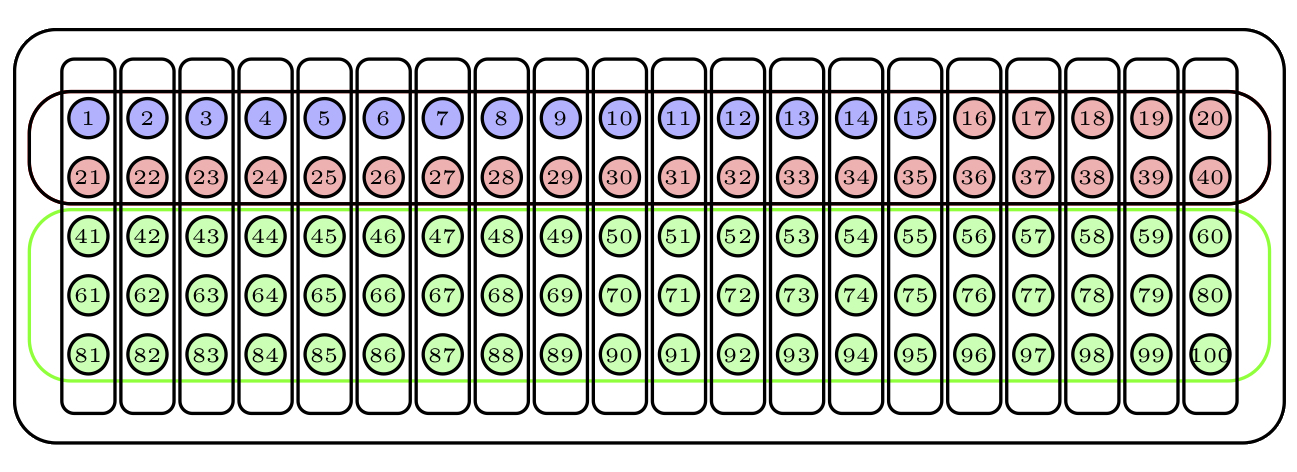
\includegraphics[width=0.8\linewidth]{INREMDN_files/figure-html/oport} 

}

\caption{Una muestra oportunista.}\label{fig:oport}
\end{figure}

\textbf{Las técnicas de estadística inferencial no se pueden aplicar a muestras no aleatorias}. Pero normalmente solo podemos conseguir muestras no aleatorias. En este caso, lo mejor es describir en detalle las características de la muestra para justificar que, pese a no ser aleatoria, podría pasar por aleatoria y es razonablemente representativa de la población. Por ejemplo, la muestra oportunista anterior de nuestra urna no es de ninguna manera representativa de su contenido por lo que refiere al color de las bolas.

\begin{rmdexercici}
Para conocer la opinión de los estudiantes de Medicina españoles sobre un tema concreto, os la pido a vosotros. ¿Qué tipo de muestreo he realizado de los explicados hasta ahora?
\end{rmdexercici}

\hypertarget{sec:poli}{%
\subsection{Muestreo polietápico}\label{sec:poli}}

En el ejemplo de los estudiantes de Primaria, la muestra final de estudiantes estaba formada por todos los de las aulas elegidas. Otra opción podría haber sido, tras seleccionar la muestra aleatoria de aulas, entrevistar solo una muestra aleatoria de estudiantes de cada una (si por ejemplo nuestro presupuesto no da para procesar las entrevistas a todos los estudiantes de las aulas elegidas). Otro ejemplo: algunos estudios poblacionales a nivel estatal se realizan solamente en algunas provincias escogidas aleatoriamente, en las que luego se encuesta una muestra aleatoria de habitantes. Los dos son ejemplos de \textbf{muestreos polietápicos}, en los que la muestra no se obtiene en un solo paso, sino mediante diversas elecciones sucesivas.

La Figura \ref{fig:poli} muestra un ejemplo sencillo de muestreo polietápico de nuestra urna: hemos elegido al azar 5 conglomerados (marcados en azul) y de cada uno de ellos hemos elegido 3 bolas al azar sin reposición.

\begin{figure}

{\centering 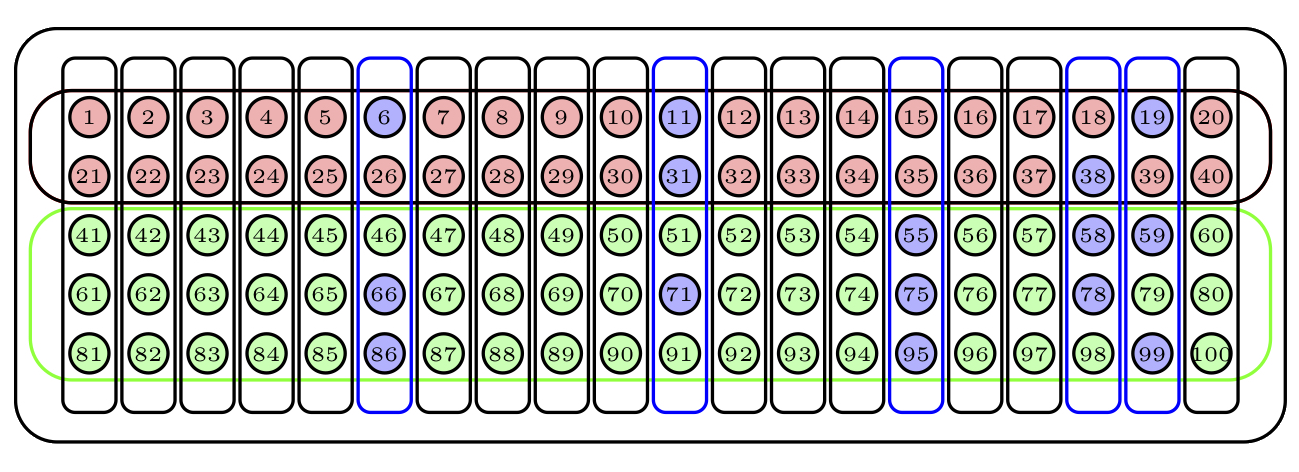
\includegraphics[width=0.8\linewidth]{INREMDN_files/figure-html/poli} 

}

\caption{Una muestra polietápica.}\label{fig:poli}
\end{figure}

Veamos algunos ejemplos más. Recordad el estudio CORSAIB del Ejemplo \ref{exm:corsaib}. Vamos a detallar algo más el proceso mediante el cual se eligieron los participantes:

\begin{enumerate}
\def\labelenumi{\arabic{enumi}.}
\item
  Se dividieron las Baleares en 14 sectores geográficos. Se ofreció la participación a los médicos de familia para conseguir que colaborasen 3-4 médicos por sector, hasta llegar a los 50 médicos.
\item
  De la población adscrita a cada médico participante se obtuvo una muestra aleatoria de 40 individuos.
\end{enumerate}

Como veis, el muestreo tuvo dos etapas. En la primera se seleccionaron clústers mediante un muestreo no aleatorio estratificado: los estratos fueron los 14 sectores geográficos, los clústers elegidos estaban formados por los grupos de pacientes adscritos a los médicos de familia que voluntariamente participaron en el estudio. La segunda etapa fue un muestreo aleatorio sin reposición dentro de cada clúster.

Veamos otro ejemplo más complicado. En el estudio \href{https://www.scielo.br/pdf/jped/v82n2/en_v82n2a08.pdf}{``Factors associated with risk of low folate intake among adolescents''} (M. Vitolo \emph{et al}, \emph{Jornal de Pediatria} 82 (2006), pp.~121--126)
los investigadores tenían que tomar una muestra de adolescentes de San Leopoldo (Brasil). Para ello:

\begin{enumerate}
\def\labelenumi{\arabic{enumi}.}
\tightlist
\item
  En primer lugar, escogieron mediante un muestreo aleatorio sistemático varias secciones censales de las 40 que tiene la ciudad.
\item
  A continuación, escogieron al azar varias manzanas de cada una de estas secciones censales y una esquina de cada manzana.
\item
  Luego, eligieron direcciones de cada manzana de manera sistemática: una de cada tres en sentido horario a partir de la esquina seleccionada.
\item
  Finalmente, se invitó a participar en el estudio a todos los habitantes de 10 a 19 años en las casas o fincas seleccionadas. El total eligible de adolescentes fueron 810, de los que aceptaron participar 722.
\end{enumerate}

En este proceso, se realizaron: un muestreo aleatorio sistemático (las secciones censales), dos muestreos aleatorios sin reposición (las manzanas y las esquinas), otro muestreo sistemático (las direcciones) y un muestreo no aleatorio (los voluntarios).

Un último ejemplo. Recordad el estudio sobre enfermedades y mes de nacimiento del Ejemplo \ref{exm:quesada}, donde ``se escogió al azar una muestra de 29,478 españoles''. En realidad, \textbf{no} se tomó una lista de toda la población española a 1 de enero de 2017 y se escogió al azar de manera equiprobable una conjunto de 29,478 personas, sino que se usó la muestra de la \emph{Encuesta Nacional de Salud} de ese año, que se elige de la manera polietápica siguiente (podéis consultar \href{https://www.ine.es/metodologia/t15/t153041917.pdf}{aquí} la metodología en detalle):

\begin{enumerate}
\def\labelenumi{\arabic{enumi}.}
\item
  Se clasifican los municipios españoles en 7 tipos según su población.
\item
  En cada comunidad autónoma y para cada tipo de municipios, se toma una muestra aleatoria de un número de secciones censales del global de esos municipios proporcional a su población.
\item
  De cada sección censal elegida, se escogen un número fijo de primeras residencias (en 2017 fueron 15) por muestreo aleatorio sistemático (y previa una ordenación específica de las viviendas según su tamaño).
\item
  En cada vivienda se escoge equiprobablemente un individuo adulto.
\end{enumerate}

Fijaos que, en (2), se toma una muestra aleatoria estratificada de secciones censales: los estratos son las combinaciones de comunidad autónoma y tipo de municipio.

Existen otros tipos de muestreo, solo hemos explicado los más comunes. En cualquier caso, lo importante es recordar que el estudio estadístico que se realice tiene que adaptarse al tipo de muestreo usado. Por ejemplo, no se pueden usar las mismas técnicas para analizar una muestra aleatoria simple que una muestra estratificada o una muestra por conglomerados. En este curso nos ocuparemos casi exclusivamente del \textbf{muestreo aleatorio simple}, es decir, al azar y con reposición, o al azar sin reposición si la población es muy grande comparada con la muestra.

\begin{rmdexercici}
Deseamos llevar a cabo un estudio para determinar si un diabético tipo 2 en las Baleares tiene una mayor probabilidad de infectarse de COVID-19 que una persona sin esa patología. Además, queremos poder comparar las probabilidades entre los diabéticos de Mallorca, de Menorca y de Ibiza. Hemos calculado que para que las conclusiones sean fiables, necesitamos analizar 50 diabéticos tipo 2 de cada isla.

Explicad en detalle cómo obtendríais la muestra de diabéticos; el procedimiento ha de ser fácil de llevar a cabo y ha de dar muestras razonablemente representativas de las poblaciones de diabéticos.
\end{rmdexercici}

\hypertarget{sec:sesgos}{%
\section{Sesgos}\label{sec:sesgos}}

Un \textbf{sesgo} es cualquier tipo de error sistemático en el diseño o la ejecución de un estudio que afecte a los datos recogidos y perjudique la corrección de las conclusiones obtenidas.

\begin{example}
\protect\hypertarget{exm:unnamed-chunk-79}{}\label{exm:unnamed-chunk-79}Si en un estudio transversal sobre hipertensión usamos un esfigmomanómetro que sistemáticamente mide una presión arterial más alta que la real, se produce un sesgo que hará que se detecte una prevalencia mayor de hipertensos que la real.
\end{example}

Los errores que pueden dar lugar a sesgos no se han de confundir con el error aleatorio inherente a las mediciones. Por ejemplo, no son sesgos los errores de medición debidos a la imprecisión del esfigmomanómetro, que mide la tensión redondeando a mm Hg, o a la variación natural de la presión arterial en un individuo a lo largo del día. La estadística nos proporciona herramientas para tratar el error aleatorio, pero las fuentes de sesgo se han de eliminar al diseñar el estudio o detectarlas al leer un estudio para valorar la validez de sus conclusiones.

Muchos autores han producido \href{https://catalogofbias.org/biases/}{listas larguísimas de tipos de sesgos} que muestran la creatividad de los humanos a la hora de fastidiarla y de poner nombres a las diferentes maneras de fastidiarla. Aquí solo vamos a introducir algunos de los más comunes. \href{https://www.scientific-european-federation-osteopaths.org/los-sesgos/}{En este \emph{url}} encontraréis una lista algo más larga, aunque tampoco es exhaustiva.

\begin{enumerate}
\def\labelenumi{\arabic{enumi}.}
\item
  \textbf{Sesgo de selección}: Se produce cuando la muestra seleccionada no es representativa de la población objetivo. Por poner un ejemplo exagerado, sería el caso si quisiéramos saber la incidencia del cáncer de ovario en una comunidad y para ello tomáramos una muestra de solo hombres.

  Hay varios subtipos que vale la pena distinguir:

  \begin{enumerate}
  \def\labelenumii{\alph{enumii}.}
  \item
    \textbf{Sesgo de falta de representatividad}: Cuando la muestra no es representativa debido a un defecto en su obtención.

    Por ejemplo, una muestra de hombres para estimar la incidencia del cáncer de ovario; o una muestra de voluntarios que se ofrezcan para que les hagan unas pruebas dolorosas a cambio de una compensación económica.

    Un ejemplo frecuente en medicina y con nombre propio (\textbf{sesgo de Berkson}) se produce cuando para estudiar la influencia de algunos factores de riesgo en una enfermedad, se toman tanto los casos como los controles entre pacientes hospitalizados. Los pacientes hospitalizados tendrán unas patologías más severas que la población en general, y puede que ello se deba a que su exposición a factores de riesgo sea mayor que la de la población en general.
  \item
    \textbf{Sesgo de selección diferencial}: Cuando el sesgo de selección se da en unos grupos sí y en otros no, o cuando se da de manera diferente en los diferentes grupos.

    Siguiendo con el ejemplo de la influencia de algunos factores de riesgo en una enfermedad que en principio no conlleve hospitalización, se daría si tomáramos los casos entre enfermos hospitalizados (que no tienen por qué ser representativos del global de enfermos) y los controles entre individuos no hospitalizados.
  \item
    \textbf{Sesgo de supervivencia}: Cuando se toma una muestra de pacientes vivos de una enfermedad con una alta tasa de mortalidad. En este caso, es muy probable que la muestra incluya una proporción muy elevada de enfermos que hayan sobrevivido más de lo normal, y estos no tienen por qué ser representativos del colectivo de enfermos de esta enfermedad.

    A veces se usa el término \textbf{sesgo de supervivencia} para describir casos como el de la Fig. \ref{fig:sesgosup}: cuando solo se consideran los sujetos que han tenido éxito en algún proceso con una tasa muy baja de éxitos (es el ``a mí me ha funcionado'' de los anuncios de remedios milagrosos e increíbles).
  \end{enumerate}
\end{enumerate}

\begin{figure}

{\centering \includegraphics[width=0.5\linewidth]{downloadFigs4latex_INREMDN/sesgosup} 

}

\caption{"Sesgo de supervivencia" (https://xkcd.com/1827/ (CC-BI-NC 2.5))}\label{fig:sesgosup}
\end{figure}

\begin{enumerate}
\def\labelenumi{\arabic{enumi}.}
\setcounter{enumi}{1}
\item
  \textbf{Sesgo de medida}: Se produce cuando el método de medición es defectuoso en algún sentido. Incluye, por ejemplo:

  \begin{enumerate}
  \def\labelenumii{\alph{enumii}.}
  \item
    \textbf{Sesgo de recuerdo}: En estudios en los que recojamos la información sobre exposición por medio de entrevistas o encuestas, existe la posibilidad de que algunos encuestados hayan olvidado información, o simplemente de que mientan en temas delicados.
  \item
    \textbf{Sesgo de recuerdo diferencial}: Es un caso particular del anterior. En estudios de casos y controles en los que recojamos la información sobre exposición por medio de entrevistas o encuestas, los casos tienen mayor tendencia a recordar su exposición a circunstancias que ellos asocien a la enfermedad que los controles.
  \item
    \textbf{Sesgo de procedimiento}: Cuando el clínico analiza de manera diferente un grupo que otro. Se daría, por ejemplo, en un ensayo clínico si se llevara a cabo un seguimiento más frecuente a los que toman un nuevo tratamiento que a los controles, por si presentan efectos secundarios inesperados.
  \item
    \textbf{Sesgo de detección}: Cuando se usan varios métodos con diferente sensibilidad para detectar una enfermedad o una exposición. Este sesgo también puede ser \textbf{diferencial} si los diferentes métodos se usan sobre grupos diferentes.

    A modo de ejemplo, se daría un sesgo de detección si para saber si los sujetos de una muestra han tomado un medicamento, a algunos se les pasa una encuesta y a otros se les consulta el historial clínico. Sería diferencial si, además, por ejemplo, los primeros fueran los participantes sanos y los segundos los enfermos.
  \item
    \textbf{Sesgo de atención}: Cuando los participantes en un estudio alteran su comportamiento porque saben que participan en un estudio (a veces se lo denomina \href{https://es.wikipedia.org/wiki/Efecto_Hawthorne}{\textbf{efecto Hawthorne}}).

    Se podría dar, por ejemplo, en un estudio sobre el efecto del ejercicio físico en la salud si los sujetos del grupo de intervención (a los que se ha asignado el hacer ejercicio físico) deciden tomar otros nuevos hábitos saludables porque saben que se les ha asignado al grupo ``saludable''. El ``efecto Hawthorne'' refiere al nombre de una fábrica en el que se realizó un estudio sobre qué condiciones aumentaban la productividad, y todos los grupos aumentaron su productividad durante el seguimiento. Este aumento se debió al efecto ``motivador'' de ser observados, porque cuando terminó el estudio volvieron todos a su productividad normal.
  \item
    \textbf{Sesgo de error instrumental}: Cuando los instrumentos usados para medir alguna característica son defectuosos. Sería el caso, por ejemplo, del esfigmomanómetro del primer párrafo de esta sección.
  \end{enumerate}
\item
  \textbf{Confusión}. Se da cuando el efecto de la exposición a un riesgo A se confunde con el de la exposición a otro factor B (el \textbf{confundidor}) que está asociado a la exposición a A y que es el verdadero causante del desenlace X que estamos estudiando.

  Hemos explicado varios ejemplos de confundidores al hablar de los problemas de los estudios de casos y controles (Sección \ref{sec:cyc}). Por ejemplo, la asociación entre que la madre sea fumadora y una disminución del riesgo de que el hijo tenga síndrome de Down, debida en realidad al factor de confusión dado por la edad de las madres (Ejemplo \ref{exm:fumarDownCC}). Por poner otro ejemplo, si en un estudio se observa una asociación entre una patología durante el embarazo y un defecto en los recién nacidos, podría ser que la causa del desenlace no fuera la enfermedad de las madres sino el tratamiento que se les hubiera admninistrado relacionado con la misma.

  Hemos incluido la confusión en la lista de sesgos, pero su naturaleza es diferente de los anteriores. Un sesgo es un error sistemático en la recolección de datos, mientras que no tener en cuenta los posibles confundidores es un error que tanto se puede cometer al diseñar el estudio como al interpretar los resultados.
\end{enumerate}

Hay muchos otros tipos de sesgos. No es importante en este curso saber sus nombres, de hecho ni tan siquiera de los que hemos dado aquí. Lo importante es aplicar el sentido común al leer la Metodología de un estudio para entender qué procesos podrían haber desviado los datos recogidos y cómo estos sesgos afectan las conclusiones del estudio.

\begin{example}
\protect\hypertarget{exm:Hola2}{}\label{exm:Hola2}Volvamos al Ejemplo \ref{exm:Hola}, en el que explicábamos el caso de una revista del corazón que, para conocer la opinión de sus lectores sobre la familia real española, propuso una encuesta en línea en su web. ¿Qué sesgos se pudieron dar?
\end{example}

\textbf{(1.a)} ¿Sesgo de falta de representatividad? Sí, claro. Los voluntarios que rellenan encuestas en Internet no tienen por qué ser representativos del total de lectores de la revista.

\textbf{(1.b)} ¿Sesgo de selección diferencial? No, porque no se eligieron dos grupos.

\textbf{(1.c)} ¿Sesgo de supervivencia? No, se supone que les interesaba conocer la opinión de sus lectores vivos en ese momento, ¿verdad?

\textbf{(2.a)} ¿Sesgo de recuerdo? Sí, claro, tenemos que tenerlo en cuenta siempre que se recoja información por medio de cuestionarios o entrevistas. Los participantes podrían haber querido dar una mejor opinión de la familia real española que la que realmente tienen para quedar bien o hacer quedar bien a la revista.

\textbf{(2.b)} ¿Sesgo de recuerdo diferencial? De nuevo, no, porque no se eligieron dos grupos.

\textbf{(2.c,d)} ¿Sesgo de procedimiento o de detección? No, por el mismo motivo

\textbf{(2.e)} ¿Sesgo de atención? No, porque no se hizo un seguimiento a los participantes, por lo que si cambiaron su comportamiento, no afectó al resultado de la encuesta.

\textbf{(2.f)} ¿Sesgo de error instrumental? Podría ser, si el cuestionario estuviera amañado en algún sentido. A lo mejor recordáis el famoso caso de la encuesta de satisfacción de Ryanair en 2017 en la que en la pregunta sobre el grado de satisfacción con su experiencia de vuelo con ellos, las únicas respuestas que se ofrecían eran ``Excelente'', ``Muy buena'', ``Buena'', ``Aceptable'' y ``OK''.

\begin{rmdromans}
No hace falta ser tan burdo a la hora de amañar un cuestionario. En una encuesta en el Reino Unido en el 2015, a la pregunta ``¿Está usted de acuerdo en permitir a los jóvenes de 16 y 17 años votar en el referéndum del Bréxit?'', un 52\% respondió que sí y un 41\% que no. Hasta ahí bien. Pero en la misma encuesta, bastantes preguntas después, se les pedía ``¿Está usted de acuerdo en reducir la edad de voto de los 18 años a los 16 en el referéndum del Bréxit?'', y a esa pregunta respondieron que sí el 37\% y que no el 56\%.
\end{rmdromans}

\begin{figure}

{\centering \includegraphics[width=0.8\linewidth]{INREMDN_files/figure-html/felipe6} 

}

\caption{¿El País marcándose un Ryanair con Felipe VI? Gráfico publicado por El País  el 30/08/2020; referencia: https://elpais.com/espana/2020-08-29/los-espanoles-rechazan-la-marcha-de-juan-carlos-i-a-emiratos-arabes.html}\label{fig:felipe6}
\end{figure}

\textbf{(3)} ¿Confusión? Dado que, por así decirlo, se trataba de un estudio transversal de prevalencia, sin intentar estimar relaciones de causa-efecto, no tiene sentido preguntarse por la existencia de confundidores. Otra cosa sería si se hubiera pretendido estudiar qué características hacen que se opine mejor o peor sobre la familia real española. Entonces sí que podrían entrar en juego confundidores. Para no meternos en berenjenales, no vamos a describirlos.

\begin{rmdexercici}
En un famoso \href{https://www.nejm.org/doi/full/10.1056/NEJM198103123041102}{estudio publicado en 1981} sobre la asociación entre consumo de café y cáncer de páncreas, se tomó un grupo formado por todos los pacientes diagnosticados de cáncer de páncreas entre 1974 y 1979 en once hospitales. Luego, para cada uno de estos casos, se pidió al médico que lo había diagnosticado que eligiera de entre sus pacientes hospitalizados más o menos al mismo tiempo uno o dos controles de características similares pero sin cáncer de páncreas. En total participaron 369 casos y 644 controles. A todos los participantes se les pidió información sobre su consumo de tabaco, alcohol, te y café. Por lo que refiere al café, se observó que los sujetos sin cáncer de páncreas de la muestra consumían menos café que los sujetos con cáncer, como podéis ver en la Figura \ref{fig:macmahon}.

¿Creéis que el consumo de café entre los controles es representativo de la población sin cáncer de páncreas? (Va, una pista: La mayoría de los casos de cáncer de páncreas son diagnosticados por digestólogos.)
\end{rmdexercici}

\begin{figure}

{\centering \includegraphics[width=0.5\linewidth]{INREMDN_files/figure-latex/macmahon-1} 

}

\caption{Proporciones de sujetos que tomaban diferentes números de tazas diarias de café en la muestra analizada por B. MacMahon *et al*, "Coffee and cancer of the pancreas".}\label{fig:macmahon}
\end{figure}

\begin{rmdexercici}
En un \href{https://ajph.aphapublications.org/doi/abs/10.2105/AJPH.83.12.1701}{estudio llevado a cabo en Sidney en su verano de 1989-90} (\emph{American Journal of Public Health} 83 (1993), pp.~1701-1706) se quiso determinar la asociación entre nadar en playas contaminadas y sufrir enfermedades infecciosas agudas. Para ello se visitaron durante varios días de verano doce playas de los alrededores de Sidney y se invitó a participar en el estudio a varios individuos en cada ocasión. Se excluyeron individuos que hubieran nadado o que hubieran sufrido alguna enfermedad infecciosa en algún momento durante los 7 días anteriores. A los que aceptaron participar en el estudio, se los llamó por teléfono al día siguiente para pedirles si habían nadado o no el día anterior y se los volvió a llamar al cabo de una semana para pedirles si habían sufrido alguna enfermedad infecciosa desde el día de playa. Si no contestaron a la primera llamada ya no se realizó la segunda llamada. En total se reclutaron 3989 sujetos, pero solo atendieron las dos llamadas 2968. Por otro lado, se midió el nivel de contaminación del agua de las playas visitadas los días en que se reclutaron bañistas en el estudio. El resultado fue que la proporción de sujetos que sufrieron alguna enfermedad infecciosa
entre los que nadaron en aguas contaminadas fue un 33\% mayor que entre los que nadaron en aguas no contaminadas, y un 116\% mayor que entre los que no nadaron.

\emph{(a)} ¿De qué tipo de estudio creéis que se trata? Justificad vuestra respuesta.

\emph{(b)} ¿Qué sesgos se pudieron dar? ¿Cómo se podrían evitar?
\end{rmdexercici}

\hypertarget{test-1}{%
\section{Test}\label{test-1}}

\textbf{(1)} En una población se quiere determinar la prevalencia de pediculosis en niños menores de 12 años. Para ello se divide la población en barrios y en cada uno de ellos se toma una muestra aleatoria de tamaño previamente determinado. ¿De qué tipo de muestreo se trata?

\begin{enumerate}
\def\labelenumi{\arabic{enumi}.}
\tightlist
\item
  Muestreo aleatorio simple.
\item
  Muestreo aleatorio estratificado.
\item
  Muestreo aleatorio por conglomerados.
\item
  Muestreo aleatorio sistemático.
\item
  Muestreo aleatorio polietápico.
\end{enumerate}

\textbf{(2)} Disponemos de las listas de todos los pacientes tratados por hipertensión en todos los centros de salud de una ciudad. Cada lista está ordenada por fecha de nacimiento. Para tomar una muestra de hipertensos, escogemos dos centros de salud al azar, y de cada uno de ellos reclutamos cada décimo paciente en su lista de hipertensos. ¿Qué tipo de muestreo hemos usado?

\begin{enumerate}
\def\labelenumi{\arabic{enumi}.}
\tightlist
\item
  Sistemático.
\item
  Aleatorio simple.
\item
  Estratificado.
\item
  Por conglomerados.
\item
  Polietápico.
\end{enumerate}

\textbf{(3)} Las mujeres que usan anticonceptivos orales acuden a revisiones ginecológicas más a menudo que las que no. Si en un estudio de cohorte retrospectivo se encontrara una asociación entre el uso de anticonceptivos orales y alguna enfermedad ginecológica, ¿a qué tipo de sesgo se podría deber?

\begin{enumerate}
\def\labelenumi{\arabic{enumi}.}
\tightlist
\item
  Sesgo de falta de representatividad.
\item
  Sesgo de recuerdo.
\item
  Sesgo de procedimiento.
\item
  Sesgo de detección.
\item
  Sesgo de atención.
\item
  Ninguno de los anteriores.
\end{enumerate}

\textbf{(4)} En un estudio de casos y controles para estudiar la asociación entre la radioterapia y el cáncer de tiroides, se estudiaron 50 casos ingresados por cáncer de tiroides y 100 controles ingresados durante el mismo período para el tratamiento de hernias. Se entrevistó a los casos, y de estas entrevistas y sus historiales médicos se obtuvo que 20 de ellos habían sido tratados con radioterapia previamente al desarrollo del cáncer de tiroides. Los controles no fueron entrevistados, pero una revisión de sus historiales médicos reveló que solo 2 de ellos habían estado expuestos a radioterapia en el pasado.

¿Qué tipo de sesgo es imposible que se dé en este estudio?

\begin{enumerate}
\def\labelenumi{\arabic{enumi}.}
\tightlist
\item
  Sesgo de recuerdo.
\item
  Sesgo de falta de representatividad, debido a que los controles no son representativos de la población sin cáncer de tiroides
\item
  Sesgo de detección, debido al uso de diferentes métodos de determinación de la exposición en los casos y controles
\item
  Sesgo de procedimiento porque el grupo de cáncer de tiroides recibirá un seguimiento más exhaustivo por parte de los médicos que el grupo de herniados.
\item
  Algún confundidor no controlado que causara en los casos la enfermedad por la que recibieron radioterapia y posteriormente el cáncer de tiroides.
\end{enumerate}

\hypertarget{part-tema-ii-probabilidades}{%
\part*{Tema II: Probabilidades}\label{part-tema-ii-probabilidades}}
\addcontentsline{toc}{part}{Tema II: Probabilidades}

\hypertarget{probabilidades-elementales-las-mates}{%
\chapter{Probabilidades elementales: Las mates}\label{probabilidades-elementales-las-mates}}

La probabilidad de un suceso es, básicamente, un número entre 0 y 1 (o, si lo preferís, un porcentaje entre 0\% y 100\%) que mide la expectativa de que se dé este suceso. En este curso vamos a definir la \textbf{probabilidad de un suceso} como la \textbf{proporción} (la \textbf{fracción}, el \textbf{porcentaje}) de sujetos de una población (o a veces de una muestra, dependerá del contexto) en los que se da el suceso. Esta proporción mide la ``probabilidad'' de que si escogemos al azar un sujeto de la población, se dé en él el suceso (y de hecho coincide con esta probabilidad, para la definición formal de probabilidad que aquí no veremos).

\begin{example}
\protect\hypertarget{exm:unnamed-chunk-83}{}\label{exm:unnamed-chunk-83}La probabilidad de que al lanzar una moneda al aire salga cara es la proporción de la población (virtual y prácticamente infinita) de lanzamientos de esta moneda en los que sale cara.
\end{example}

En casos MUY sencillos, cuando \textbf{todos los resultados posibles tienen la misma probabilidad}, esta proporción coincide con la fracción de veces en que se da este suceso en el conjunto de resultados posibles y por lo tanto se puede calcular con la famosa \textbf{regla de Laplace}:
\[
\text{Probabilidad}=\frac{\text{Casos favorables}}{\text{Casos posibles}}
\]

Por ejemplo:

\begin{itemize}
\item
  La probabilidad de que salga cara al lanzar una moneda equilibrada al aire es 1/2 (casos favorables, 1; casos posibles, 2; los dos resultados tienen la misma probabilidad por definición de moneda equilibrada).
\item
  Pero la probabilidad de que un hijo sea varón no es 1/2, aunque solo haya dos sexos anatómicos. Es la proporción de hijos varones en el total de todos los hijos, que se estima en alrededor del 51.22\%.
\item
  O más exageradamente, la probabilidad de que una mujer de entre 17 y 27 años sea miope no es 1/2, aunque solo haya dos resultados posibles: ser miope y no serlo. Esta probabilidad es la proporción de miopes en la población formada por todas las mujeres de esa franja de edad, que, en España en 2018, se estimaba en un 65.4\% según un \href{http://visionyvida.org/informe-prevalencia-de-la-miopia-en-los-jovenes-en-espana-2018/}{informe de la Asociación Visión y Vida}.
\end{itemize}

\begin{rmdromans}
Si lanzamos al aire dos veces seguidas una moneda equilibrada, ¿cuál es la probabilidad de que salga alguna cara?

Según el enciclopedista y matemático \href{https://es.wikipedia.org/wiki/Jean_le_Rond_d\%27Alembert}{J. d'Alembert} es 2/3. Su argumento era el siguiente. Si en el primer lanzamiento sale cara, ya tenemos una cara. Si sale cruz, volvemos a lanzar otra vez y miramos si sale cara o cruz. Por lo tanto, hay solo 3 resultados posibles: cara en el primer lanzamiento; cruz en el primer lanzamiento y cara en el segundo; cruz en ambos lanzamientos. De estos tres ``casos posibles'', solo en los 2 primeros sale alguna cara. Casos favorables partido por casos posibles: 2/3.

¿Es correcto este argumento?
\end{rmdromans}

La teoría matemática de las probabilidades es la que nos permite valorar lo exacta que es una estimación de un valor para una población a partir de una muestra. Por ejemplo, supongamos que elegimos al azar un grupo de 50 estudiantes de la UIB y observamos que 33 sufren de miopía. A partir de este dato, vamos a estimar que un 66\% de los estudiantes de la UIB son miopes. ¿Hasta qué punto nos podemos fiar de esta estimación? La teoría de las probabilidades nos permitirá calcular la probabilidad de acertar con esta estimación más o menos un margen de error fijado.

\hypertarget{uxe1lgebra-de-conjuntos}{%
\section{Álgebra de conjuntos}\label{uxe1lgebra-de-conjuntos}}

Vamos a repasar muy rápidamente las notaciones y las propiedades de las operaciones de conjuntos, para poder usar este lenguaje en lo que sigue.

Sean \(A\) y \(B\) subconjuntos (en el contexto de la teoría de probabilidades, se los llama \textbf{sucesos}) de un conjunto \(\Omega\) (nuestra \textbf{población} o, en el lenguaje de la teoría de probabilidades, el \textbf{espacio muestral}).

\begin{itemize}
\item
  \(A\cup B\) es la \textbf{unión} de \(A\) y \(B\): el conjunto formado por los elementos de \(\Omega\) que pertenecen a \(A\) o a \(B\) (o a ambos).

  Corresponde a la \textbf{disjunción} del lenguaje natural.
\end{itemize}

\begin{rmdimportant}
En este curso la disjunción ``o'' nunca es exclusiva, salvo cuando digamos explícitamente que lo es mediante expresiones del tipo de ``o A o B pero no ambos''.
\end{rmdimportant}

\begin{itemize}
\item
  \(A \cap B\) es la \textbf{intersección} de \(A\) y \(B\): el conjunto formado por los elementos que pertenecen simultáneamente a \(A\) y a \(B\).

  Corresponde a la \textbf{conjunción} del lenguaje natural.
\item
  \(A^c\) es el \textbf{complementario} de \(A\): el conjunto formado por los elementos de \(\Omega\) que no pertenecen a \(A\).

  Corresponde a la \textbf{negación} del lenguaje natural.
\item
  \(A-B=A \cap B^c\) es la \textbf{diferencia} ``\(A\) menos \(B\)'': el conjunto formado por los elementos de \(A\) que no pertenecen a \(B\).

  Por lo tanto, \(A^c=\Omega-A\).
\item
  Diremos que \(A\) y \(B\) son \textbf{disjuntos}, o \textbf{incompatibles}, cuando \(A\cap B=\emptyset\), donde \(\emptyset\) es el \textbf{conjunto vacío}, el conjunto que no tiene elementos.
\item
  Diremos que \(A\) está \textbf{contenido}, o \textbf{incluido}, en \(B\), y lo denotaremos por \(A\subseteq B\), cuando todo elemento de \(A\) pertenece a \(B\). Para recalcar que \(A\) está \textbf{estrictamente contenido} en \(B\) (que está contenido en \(B\) pero no es igual a \(B\)) usaremos \(A\subsetneq B\).
\end{itemize}

\begin{example}
\protect\hypertarget{exm:unnamed-chunk-86}{}\label{exm:unnamed-chunk-86}Consideremos la población \(\Omega\) formada por los estudiantes de una clase, y sean \(A\) el subconjunto formado por la mujeres de esa clase y \(B\) el subconjunto formado por los estudiantes de esa clase que llevan gafas.
\end{example}

Entonces:

\begin{itemize}
\item
  \(A\cup B\) es el conjunto de los estudiantes de la clase que son mujeres o llevan gafas.
\item
  \(A \cap B\) es el conjunto de los estudiantes de la clase que son mujeres y llevan gafas, es decir, las mujeres de la clase que llevan gafas.
\item
  \(A^c\) es el conjunto de los estudiantes de la clase que no son mujeres, es decir los hombres de la clase.
\item
  \(B^c\) es el conjunto de los estudiantes de la clase que no llevan gafas.
\item
  \(A-B\) es el conjunto de las mujeres de la clase que no llevan gafas.
\item
  \(B-A\) es el conjunto de los estudiantes de la clase que llevan gafas y no son mujeres, es decir, los hombres de la clase que llevan gafas.
\item
  \(A\) y \(B\) serán disjuntos (llevar gafas y ser mujer serán incompatibles en esta clase) si no hay ninguna mujer en la clase que lleve gafas.
\item
  \(A\subseteq B\) será verdad si todas las mujeres de la clase llevan gafas.
\item
  \(B\subseteq A\) será verdad si todos los estudiantes de la clase que llevan gafas son mujeres.
\end{itemize}

Las propiedades de estas operaciones son las siguientes, y se corresponden a las propiedades de las conjunciones, disjunciones y negaciones en el lenguaje natural.

\begin{enumerate}
\def\labelenumi{\alph{enumi}.}
\item
  \textbf{Absorción}: Si \(A\subseteq B\), entonces \(A\cap B=A\) y \(A\cup B=B\).
\item
  La unión y la intersección son \textbf{conmutativas}: \(A\cup B=B\cup A\) y \(A\cap B=B\cap A\).
\item
  La unión y la intersección son \textbf{asociativas}: \(A\cup(B\cup C)=(A\cup B)\cup C\) y \(A\cap(B\cap C)=(A\cap B) \cap C\).
\end{enumerate}

\begin{figure}

{\centering \includegraphics[width=0.8\linewidth]{INREMDN_files/figure-html/assocunio} 

}

\caption{Propiedad asociativa de la unión.}\label{fig:unnamed-chunk-87}
\end{figure}

\begin{figure}

{\centering \includegraphics[width=0.8\linewidth]{INREMDN_files/figure-html/assocint} 

}

\caption{Propiedad asociativa de la intersección.}\label{fig:unnamed-chunk-88}
\end{figure}

\begin{enumerate}
\def\labelenumi{\alph{enumi}.}
\setcounter{enumi}{3}
\tightlist
\item
  La unión y la intersección son \textbf{distributivas}: \(A\cap(B\cup C)=(A\cap B)\cup (A\cap C)\) y \(A\cup(B\cap C)=(A\cup B)\cap (A\cup C)\).
\end{enumerate}

\begin{figure}

{\centering \includegraphics[width=0.8\linewidth]{INREMDN_files/figure-html/distr1BD} 

}

\caption{Propiedad distributiva de la unión respecto de la intersección.}\label{fig:unnamed-chunk-89}
\end{figure}

\begin{figure}

{\centering \includegraphics[width=0.8\linewidth]{INREMDN_files/figure-html/distr2BD} 

}

\caption{Propiedad distributiva de la intersección respecto de la unión.}\label{fig:unnamed-chunk-90}
\end{figure}

\begin{enumerate}
\def\labelenumi{\alph{enumi}.}
\setcounter{enumi}{4}
\item
  Propiedad del \textbf{doble complementario}: \((A^c)^c=A\).

  Corresponde a que, en el lenguaje natural, ``No es verdad que no lleve gafas'' significa lo mismo que ``Lleva gafas''.
\end{enumerate}

\begin{figure}

{\centering \includegraphics[width=0.8\linewidth]{INREMDN_files/figure-html/dcBD} 

}

\caption{Propiedad del doble complementario.}\label{fig:unnamed-chunk-91}
\end{figure}

\begin{enumerate}
\def\labelenumi{\alph{enumi}.}
\setcounter{enumi}{5}
\item
  \textbf{Leyes de De Morgan}: \((A\cup B)^c=A^c \cap B^c\) y \((A\cap B)^c=A^c\cup B^c\).

  La primera corresponde a que, en el lenguaje natural, lo contrario de ``Ser mujer o llevar gafas'' es ``No ser mujer \textbf{Y} no llevar gafas''. La segunda, a que lo contrario de ``Ser mujer y llevar gafas'' es ``No ser mujer \textbf{O} no llevar gafas''.
\end{enumerate}

\begin{figure}

{\centering \includegraphics[width=0.8\linewidth]{INREMDN_files/figure-html/dM1BD} 

}

\caption{Una ley de de Morgan.}\label{fig:unnamed-chunk-92}
\end{figure}

\begin{figure}

{\centering \includegraphics[width=0.8\linewidth]{INREMDN_files/figure-html/dM2BD} 

}

\caption{La otra ley de de Morgan.}\label{fig:unnamed-chunk-93}
\end{figure}

Que la unión y la intersección sean asociativas y conmutativas nos permite escribir expresiones del estilo de
\[
A_1\cap A_2\cap \cdots \cap A_n,\qquad A_1\cup A_2\cup \cdots \cup A_n
\]
para indicar, respectivamente, la intersección o la unión de los sucesos \(A_1,\ldots,A_n\) agrupándolos como queramos y en el orden que queramos.

\hypertarget{algunas-fuxf3rmulas-buxe1sicas}{%
\section{Algunas fórmulas básicas}\label{algunas-fuxf3rmulas-buxe1sicas}}

Hemos definido la probabilidad \(P(A)\) de un subconjunto (suceso) \(A\) de una población (espacio muestral) \(\Omega\) como la fracción de los sujetos de \(\Omega\) que pertenecen a \(A\). A partir de esta definición se deducen, por puro conteo, las propiedades siguientes:

\begin{enumerate}
\def\labelenumi{\arabic{enumi}.}
\item
  Para todo suceso \(A\), \(0\leqslant P(A)\leqslant 1\).

  Un subconjunto \(A\) de \(\Omega\) no puede representar ni una fracción negativa ni una fracción mayor que 1 de los sujetos de \(\Omega\).
\item
  \(P(\Omega)=1\) y \(P(\emptyset)=0\) (recordad que \(\emptyset\) es el conjunto vacío).
\item
  Si \(A\) y \(B\) son dos sucesos disjuntos, entonces \(P(A\cup B)=P(A)+P(B)\).

  Si no hay ningún sujeto que pertenezca simultáneamente a \(A\) y a \(B\), entonces el número de sujetos que pertenecen a \(A\) o a \(B\) es la suma de los que pertenecen a \(A\) y de los que pertenecen a \(B\). Entonces, dividiendo por el número total de individuos de la población \(\Omega\) (su \textbf{cardinal}), obtenemos que la fracción de los sujetos que pertenecen a \(A\) o a \(B\) es la suma de las fracciones de los que pertenecen a \(A\) y de los que pertenecen a \(B\).
\item
  Más en general, si \(A_1,A_2,\ldots,A_n\) son sucesos disjuntos dos a dos, entonces
  \[
  P(A_1\cup A_2\cup \cdots \cup A_n)=P(A_1)+P(A_2)+\cdots +P(A_n).
  \]
\item
  \(P(A-B)=P(A)-P(A\cap B)\).

  El número de sujetos que pertenecen a \(A\) pero no a \(B\) se obtiene restando del total de sujetos de \(A\) los que pertenecen simultáneamente a \(A\) y a \(B\), es decir, a \(A\cap B\). Dividiendo por el número total de individuos de la población, obtenemos la correspondiente igualdad de proporciones.
\end{enumerate}

\begin{rmdcorbes}
Formalmente, como \(A-B\) y \(A\cap B\) son disjuntos (ya que ningún elemento de \(A-B\) pertenece a \(B\) y todos los elementos de \(A\cap B\) pertenecen a \(B\)), la propiedad (3) nos dice que
\[
P((A-B)\cup (A\cap B))=P(A-B)+P(A\cap B).
\]
Por otro lado, \((A-B)\cup (A\cap B)=A\) porque \(A\) es la unión del conjunto de sus elementos que no pertenecen a \(B\) y del conjunto de sus elementos que sí pertenecen a \(B\).
\end{rmdcorbes}

\begin{figure}

{\centering \includegraphics[width=0.5\linewidth]{INREMDN_files/figure-html/A-B2} 

}

\caption{Descomposición de A en dos conjuntos disjuntos.}\label{fig:AmenysB2}
\end{figure}

\begin{rmdcaution}
¡Ojo! En general, es falso que \(P(A-B)=P(A)-P(B)\). Si en una población hay un 50\% de mujeres y un 60\% de miopes, y un 35\% del total son mujeres miopes, las mujeres no miopes son un 15\% del total de la población, no un -10\%, ¿verdad?
\end{rmdcaution}

\begin{enumerate}
\def\labelenumi{\arabic{enumi}.}
\setcounter{enumi}{5}
\item
  \(P(A^c)=1-P(A)\).

  Es decir, la fracción de los sujetos que no pertenecen a \(A\) es 1 menos la fracción de los que sí pertenecen a \(A\).
\item
  Si \(A\subseteq B\), entonces \(P(A)\leqslant P(B)\).

  Si \(A\) está contenido en \(B\), la fracción de los sujetos que pertenecen a \(A\) menor o igual que la de los que pertenecen a \(B\).
\item
  \(P(A\cup B)=P(A)+P(B)-P(A \cap B)\).

  Si queréis contar cuántos sujetos hay en \(A\cup B\), tenéis que añadir a los de \(A\) los de \(B-A\) (mirad la Figura \ref{fig:AmenysB}). Dividiendo por el total de la población para pasar a proporciones, esto nos dice que
  \[
  P(A\cup B)=P(A)+P(B-A)=P(A)+P(B)-P(A \cap B)
  \]
  donde la segunda igualdad se debe a (5).

  Por ejemplo, si en una población hay un 50\% de mujeres y un 60\% de miopes, y un 35\% del total son mujeres miopes, las personas que son mujeres o miopes (recordad, o ambas cosas) forman un 75\% de la población: al 50\% de mujeres hay que sumarle el 25\% de miopes que no son mujeres.
\end{enumerate}

\begin{figure}

{\centering \includegraphics[width=0.5\linewidth]{INREMDN_files/figure-html/A-B} 

}

\caption{Descomposición de la unión en tres conjuntos disjuntos.}\label{fig:AmenysB}
\end{figure}

\begin{enumerate}
\def\labelenumi{\arabic{enumi}.}
\setcounter{enumi}{8}
\tightlist
\item
  Otra manera de escribir la ecuación anterior es
  \[
  P(A\cap B)=P(A)+P(B)-P(A \cup B)
  \]
\end{enumerate}

\begin{rmdcaution}
En general, es falso que \(P(A\cap B)=P(A)\cdot P(B)\). Por ejemplo, en la población con un 50\% de mujeres, un 60\% de miopes y un 35\% de mujeres miopes que hemos usado antes, 0.6·0.5 no es igual a 0.35.

Más adelante veremos cuándo esta igualdad es verdadera.
\end{rmdcaution}

\begin{example}
\protect\hypertarget{exm:VIHherpes1}{}\label{exm:VIHherpes1}Supongamos que el 0.1\% de los donantes de sangre dan positivo en el test de VIH, que el 1\% dan positivo en el test de herpes simple (VHS) y que el 0.05\% dan positivo en ambos tests.

¿Cuál es la probabilidad de que un donante escogido al azar dé positivo en al menos uno de los dos tests? ¿Y la de que un donante escogido al azar dé positivo en VHS pero no en VIH?
\end{example}

Vamos a poner nombres a los sucesos involucrados en estas preguntas:

\begin{itemize}
\item
  \(A\): Dar positivo en VIH. Sabemos que \(P(A)=0.001\).
\item
  \(B\): Dar positivo en VHS. Sabemos que \(P(B)=0.01\).
\item
  \(A\cap B\): Dar positivo en los dos. Sabemos que \(P(A\cap B)=0.0005\).
\item
  \(A\cup B\): Dar positivo en al menos uno de los dos. Es lo que queremos calcular en la primera pregunta.

  Por la propiedad (8):
  \[
  P(A \cup B) =P(A)+P(B)-P(A\cap B)=0.001+0.01-0.0005=0.0105
  \]
  La probabilidad de que un donante escogido al azar dé positivo en al menos uno de los dos tests es del 1.05\%.
\item
  \(B-A\): Dar positivo en VHS pero no en VIH. Es lo que queremos calcular en la segunda pregunta.

  Por la propiedad (5),
  \[
  P(B-A)=P(B)-P(A\cap B)=0.01-0.0005=0.0095
  \]
  La probabilidad de que un donante escogido al azar dé positivo en VHS pero no en VIH es del 0.95\%.
\end{itemize}

Otra manera de calcular estas probabilidades sin necesidad de recordar fórmulas sería:

\begin{itemize}
\item
  Tomar como referencia una población de un tamaño concreto.
\item
  Calcular en esta población cuántos individuos pertenecen a \(A\cap B\) (dan positivo en ambos tests), cuántos a \(A-B\) (positivos en VIH pero no en VHS), cuántos a \(B-A\) (positivos en VHS pero no en VIH) y cuántos a \(A^c\cap B^c\) (negativo en ambos tests) y a partir de ahí calcular todo lo que queramos.
\end{itemize}

A este método se le suele llamar \textbf{método de frecuencias naturales} (``la cuenta de la vieja'' no suena lo suficientemente científico), y así lo llamaremos nosotros. Pongámoslo en práctica en nuestro caso:

\begin{enumerate}
\def\labelenumi{\arabic{enumi}.}
\item
  Vamos a tomar una población de referencia de 10,000 donantes

  ¿Por qué este número? Veamos, fijaos en que la proporción de sujetos en \(A\cap B\) es del 0.05\%, es decir, 0.0005, y para facilitar los cálculos nos gustaría que todos los números que nos salieran fueran enteros, para no liarnos con decimales. Como 0.0005·10000=5, parece que 10,000 nos va a valer.
\item
  Los sujetos de \(A\) son el 0.1\% de la población: 10
\item
  Los sujetos de \(B\) son el 1\% de la población: 100
\item
  Los sujetos de \(A\cap B\) son el 0.05\% de la población: 5
\item
  Entonces, los sujetos de \(A-B\) serán los de \(A\) menos los de \(A\cap B\): 5
\item
  Y los sujetos de \(B-A\) serán los de \(B\) menos los de \(A\cap B\): 95
\item
  Por ahora ya tenemos: 5 sujetos positivos en VIH y en VHS; 5 positivos en VIH y negativos en VHS; y 95 positivos en VHS y negativos en VIH. En total, 105 sujetos. El resto serán negativos tanto en VIH como en VHS.

  Por lo tanto, los sujetos de \(A^c\cap B^c\) serán 10000-105=9895.
\end{enumerate}

Obtenemos la tabla de frecuencias siguiente:
\[
\begin{array}{r|c|c|c}
& A\ (\text{VIH}+) & A^c \ (\text{VIH}-)  & \text{Total} \\ \hline
B\ (\text{VHS}+) &  5  &  95  &   100 \\ \hline
B^c\ (\text{VHS}-) &  5  &   9895  &   9900 \\ \hline 
\text{Total} & 10& 9990 & 10000  \\ 
\end{array}
\]

Y ahora, cambiando ``probabilidad'' por ``proporción'', ya podemos calcular lo que queramos.

\begin{itemize}
\item
  ¿Cuál es la proporción de sujetos que dan positivo en algún test?

  Hay 105 sujetos en la tabla que dan positivo en algún test: los 10 positivos en VIH y los 95 positivos en VHS y negativos en VIH. Por lo tanto, su proporción es de 105/10000=0.0105.
\item
  ¿Cuál es la proporción de sujetos que dan positivo en VHS pero no en VIH?

  Hay 95 sujetos en la tabla que dan positivo en VHS y negativo en VIH, por lo que su proporción es de 95/10000=0.0095.
\end{itemize}

\begin{rmdexercici}
Seguimos en la situación anterior: el 0.1\% de los donantes de sangre dan positivo en el test de VIH, el 1\% dan positivo en el test de herpes y el 0.05\% dan positivo en los dos tests.

¿Cuál es la probabilidad de que un donante escogido al azar dé positivo en un solo test?
\end{rmdexercici}

\begin{rmdexercici}
Supongamos ahora que el 0.1\% de todos los donantes de sangre da positivo en el test de VIH, el 1\% da positivo en el test de herpes y el 1.07\% da positivo en al menos uno de los dos tests.

¿Cuál es la probabilidad de que un donante escogido al azar dé positivo en ambos tests? ¿Y la de que dé positivo en un solo test?
\end{rmdexercici}

\begin{rmdexercici}
Y supongamos ahora que el 0.1\% de todos los donantes de sangre da positivo en el test de VIH, el 1\% da positivo en el test de herpes y el 1.2\% da positivo en al menos uno de los dos tests.

¿Cuál es la probabilidad de que un donante escogido al azar dé positivo en ambos tests? ¿Y la de que dé positivo en un solo test?
\end{rmdexercici}

\begin{figure}

{\centering \includegraphics[width=0.5\linewidth]{INREMDN_files/figure-html/batmanprobs} 

}

\caption{¡Cuidado con lo que respondéis!}\label{fig:unnamed-chunk-100}
\end{figure}

\begin{example}
\protect\hypertarget{exm:repes}{}\label{exm:repes}En la Sección \ref{sec:mas} hemos dado las probabilidades de que se escoja más de una vez algún individuo en algunas situaciones. Por ejemplo, si escogemos 100 individuos de las Baleares (suponiendo que su población es de 1,150,000 habitantes) al azar permitiendo repeticiones. ¿Cómo se calculan estas probabilidades?
\end{example}

Vamos a suponer que escogemos los individuos uno tras otro. El plan va a ser calcular primero la probabilidad \(p\) de que todos los individuos de la muestra sean diferentes. Entonces, la probabilidad de que salga al menos uno repetido será \(1-p\).

Como, en el muestreo aleatorio simple, todos los grupos de 100 baleares (con posibles repeticiones) tienen la misma probabilidad de ser elegidos, podemos usar la fórmula de Laplace ``casos favorables partido por casos posibles'' para calcular \(p\). Solo hay que identificar cuántos casos favorables y cuántos casos posibles hay.

\begin{itemize}
\item
  \emph{Casos favorables}. ¿De cuántas maneras podemos elegir 100 baleares, uno tras otro, de manera que todos sean diferentes?

  \begin{itemize}
  \tightlist
  \item
    El primero puede ser cualquiera: hay 1,150,000 posibilidades.
  \item
    Una vez hemos elegido el primero, como el segundo ha de ser diferente, puede ser cualquiera de los 1,149,999 restantes.
  \item
    Una vez hemos elegido los dos primeros, como el tercero ha de ser diferente de ellos, lo podemos escoger de los 1,149,998 restantes.
  \item
    En general, cuando hemos elegido \emph{n} sujetos, el siguiente puede ser cualquiera de los 1,150,000-\emph{n} restantes.
  \item
    Y así, cuando hemos elegido los 99 primeros, para el último, el centésimo, tenemos 1,150,000-99=1,149,901 posibilidades.
  \end{itemize}
\end{itemize}

Por lo tanto hay
\[
1150000\times 1149999\times 1149998\times \cdots\times 1149901
\]
posibles elecciones de 100 baleares \textbf{diferentes}.

\begin{itemize}
\item
  \emph{Casos posibles}. ¿De cuántas maneras podemos elegir 100 baleares, uno tras otro, sin ninguna restricción?

  \begin{itemize}
  \tightlist
  \item
    El primero puede ser cualquiera: hay 1,150,000 posibilidades.
  \item
    Una vez hemos elegido el primero, como el segundo puede ser cualquiera, de nuevo tenemos 1,150,000 posibilidades para él.
  \item
    Una vez hemos elegido los dos primeros, como el tercero puede ser cualquiera, seguimos teniendo 1,150,000 posibilidades.
  \item
    En general, cuando hemos elegido \emph{n} sujetos, para el siguiente volvemos a tener 1,150,000 posibilidades.
  \end{itemize}
\end{itemize}

Por lo tanto hay
\[
\overbrace{1150000\times 1150000\times 1150000\times \cdots\times 1150000}^{100}=1150000^{100}
\]
posibles elecciones de 100 baleares sin ninguna restricción.

Por la fórmula de Laplace, la probabilidad \(p\) de que al elegir al azar 100 baleares nos salgan todos diferentes es
\[
p=\frac{1150000\times 1149999\times\cdots\times 1149901}{1150000^{100}}
\]
y, finalmente, la probabilidad de que al elegir al azar 100 baleares nos salga alguno repetido es
\[
1-p=1-\frac{1150000\times 1149999\times\cdots\times 1149901}{1150000^{100}}
\]
Naturalmente, os va a costar calcular este número con una calculadora científica sencilla, pero para eso están los ordenadores. Da 0.0042952.

R dispone de dos funciones relacionadas con la probabilidad de que se dé alguna repetición en una muestra aleatoria simple de un tamaño dado:

\begin{itemize}
\item
  La instrucción \texttt{pbirthday(n,N)} nos da la probabilidad de que en una muestra aleatoria simple de tamaño n de una población de tamaño N haya algún elemento repetido.
\item
  La instrucción \texttt{qbirthday(p,N)} nos da el tamaño mínimo de una muestra aleatoria simple de una población de tamaño N para que la probabilidad de que haya algún elemento repetido sea \(\geqslant p\).
\end{itemize}

El nombre \texttt{birthday} hace referencia a la \textbf{paradoja del cumpleaños}: el típico problema de calcular la probabilidad de que dos estudiantes de una clase celebren el cumpleaños el mismo día y asombrarse de que en una clase de 50 estudiantes haya más de un 95\% de probabilidades de que haya algún cumpleaños repetido.

En efecto, podemos entender una clase de 50 estudiantes como una muestra aleatoria simple de 50 fechas de nacimiento, escogidas de un conjunto de 366 posibles fechas (los 366 días de un año bisiesto). La probabilidad de que al menos 2 estudiantes celebren el cumpleaños el mismo día es la probabilidad de que se dé al menos una repetición en esta muestra. R lo calcula con:

\begin{Shaded}
\begin{Highlighting}[]
\FunctionTok{pbirthday}\NormalTok{(}\DecValTok{50}\NormalTok{,}\DecValTok{366}\NormalTok{)}
\end{Highlighting}
\end{Shaded}

\begin{verbatim}
## [1] 0.9700731
\end{verbatim}

La probabilidad de que en una muestra aleatoria simple de 100 ciudadanos de las Baleares se dé alguna repetición se puede calcular mediante

\begin{Shaded}
\begin{Highlighting}[]
\FunctionTok{pbirthday}\NormalTok{(}\DecValTok{100}\NormalTok{,}\DecValTok{1150000}\NormalTok{)}
\end{Highlighting}
\end{Shaded}

\begin{verbatim}
## [1] 0.004295221
\end{verbatim}

\begin{rmdexercici}
Comprobad que las otras probabilidades de repeticiones anunciadas en la lección anterior son correctas.
\end{rmdexercici}

\begin{rmdexercici}
¿Cuál es el número mínimo de estudiantes en la clase para que la probabilidad de que se repita una fecha de cumpleaños sea al menos del 95\%?
\end{rmdexercici}

\hypertarget{sec:odds}{%
\section{Odds}\label{sec:odds}}

En algunos contextos, las probabilidades se presentan en forma de \textbf{odds} (la traducción más común en castellano es \href{https://es.wikipedia.org/wiki/Apuesta_deportiva\#Momios_o_Cuotas_Deportivas}{\textbf{momios}}, pero se usan otras: posibilidades, oportunidades, ocasiones\ldots). Las \textbf{odds} de un suceso \(A\) son
\[
\text{Odds}(A)=\frac{P(A)}{P(A^c)}=\frac{P(A)}{1-P(A)}
\]
y por lo tanto nos dicen cuántas veces es más probable \(A\) que ``no \(A\)''.

\begin{figure}

{\centering \includegraphics[width=0.5\linewidth]{INREMDN_files/figure-html/catmummies} 

}

\caption{Momios de gatitos en el British Museum (fotografía de M. Sánchez).}\label{fig:catmummies}
\end{figure}

Si \(\text{Odds}(A)=q\), significa que \textbf{por cada vez que ocurre ``no \(A\)'', ocurre \(q\) veces \(A\)}. Por ejemplo, si las \emph{odds} de suspender una asignatura son 2/3, significa que:

\begin{itemize}
\tightlist
\item
  Por cada estudiante que aprueba, hay 2/3 de estudiante que suspenden.
\item
  Por cada 3 estudiantes que aprueban, hay 2 que suspenden.
\item
  De cada 5 estudiantes, 3 aprueban y 2 suspenden.
\item
  2 de cada 5 estudiantes suspenden.
\item
  La \textbf{probabilidad} de suspender es de un 40\%.
\end{itemize}

\begin{rmdnote}
A veces, que unas \emph{odds} valgan \(a/b\) se expresa diciendo que son \(a\!:\!b\), y se lee ``\(a\) a \(b\)''. Por ejemplo, las \emph{odds} de suspender anteriores son 2:3, es decir, 2 a 3.
\end{rmdnote}

\begin{example}
\protect\hypertarget{exm:unnamed-chunk-106}{}\label{exm:unnamed-chunk-106}

Algunos ejemplos de \emph{odds} a partir de probabilidades:

\begin{itemize}
\tightlist
\item
  Si \(P(A)=0.2\), \(\text{Odds}(A)=0.2/0.8=0.25\).
\item
  Si \(P(A)=0\), \(\text{Odds}(A)=0\).
\item
  Si \(P(A)=0.5\), \(\text{Odds}(A)=1\).
\item
  Si \(P(A)=1\), \(\text{Odds}(A)=\infty\).
\end{itemize}

\end{example}

Como son un cociente de dos probabilidades, las \emph{odds} de un suceso son siempre mayores o iguales que 0 y pueden tomar cualquier valor entre 0 e \(\infty\), ambos incluidos.

\begin{rmdexercici}
Si lanzamos un dado equilibrado de 10 caras numeradas del 0 al 9:

\begin{enumerate}
\def\labelenumi{\arabic{enumi}.}
\item
  ¿Qué valen las \emph{odds} de sacar un 3?
\item
  ¿Qué valen las \emph{odds} de sacar un múltiplo de 3?
  \end{rmdexercici}
\end{enumerate}

Si sabemos las \emph{odds} de \(A\), podemos calcular la probabilidad \(P(A)\):
\[
\begin{array}{rl}
\text{Odds}(A)=\dfrac{P(A)}{1-P(A)}\!\!\!\! & \Longrightarrow \text{Odds}(A)-\text{Odds}(A)P(A)=P(A)\\ 
& \Longrightarrow P(A)=\dfrac{\text{Odds}(A)}{1+\text{Odds}(A)}
\end{array}
\]

Por lo tanto, dos sucesos tienen la misma probabilidad si, y solo si, tienen las mismas \emph{odds}.

Observad que la función
\[
x\mapsto\frac{x}{1+x}
\]
es creciente en \(x\):

\begin{figure}

{\centering \includegraphics[width=0.5\linewidth]{INREMDN_files/figure-latex/unnamed-chunk-108-1} 

}

\caption{Gráfica de la curva y=x/(1+x).}\label{fig:unnamed-chunk-108}
\end{figure}

Como esta es la función que transforma \(\text{Odds}(A)\) en \(P(A)\), deducimos que
\[
\text{Odds}(A)>\text{Odds}(B)\Longleftrightarrow P(A)>P(B)
\]
Es decir, \(A\) es más probable que \(B\) si, y solo si, las \emph{odds} de \(A\) son mayores que las de \(B\).

Como veremos en la Sección \ref{sec:riesgosCyC}, la manera correcta de presentar los resultados en los estudios de casos y controles es en forma de \emph{odds ratios}. La \textbf{odds ratio} (\textbf{razón de momios}, de oportunidades\ldots) de dos sucesos \(A\) y \(B\) es el cociente de sus \emph{odds}:
\[
\text{OR}(A,B)=\frac{\text{Odds}(A)}{\text{Odds}(B)}
\]
Es decir, \(\text{OR}(A,B)\) nos dice cuántas veces son mayores (o menores) las \emph{odds} de \(A\) que las de \(B\). Su valor es difícil de interpretar en términos de probabilidades excepto por lo que refiere a su relación con 1:

\begin{itemize}
\item
  \(\text{OR}(A,B)=1\Longleftrightarrow \text{Odds}(A)=\text{Odds}(B) \Longleftrightarrow P(A)=P(B)\)
\item
  \(\text{OR}(A,B)>1\Longleftrightarrow \text{Odds}(A)>\text{Odds}(B) \Longleftrightarrow P(A)>P(B)\)
\item
  \(\text{OR}(A,B)<1\Longleftrightarrow \text{Odds}(A)<\text{Odds}(B) \Longleftrightarrow P(A)<P(B)\)
\end{itemize}

Pero, por ejemplo
\[
\text{OR}(A,B)=2 \Longleftrightarrow \text{Odds}(A)= 2\cdot \text{Odds}(B) \hspace{1.2ex}
\not\hspace{-1.2ex}\Longleftrightarrow P(A)=
2\cdot P(B)
\]

\begin{rmdcorbes}
En general, si \(\text{OR}(A,B)=q\), es decir, \(\text{Odds}(A)=q\cdot\text{Odds}(B)\), entonces
\[
\begin{array}{l}
P(A)=\dfrac{\text{Odds}(A)}{1+\text{Odds}(A)}=\dfrac{q\cdot\text{Odds}(B)}{1+q\cdot\text{Odds}(B)}\\
\qquad =\dfrac{q\cdot\frac{ P(B)}{1-P(B)}}{1+q\cdot\frac{P(B)}{1-P(B)}}=\dfrac{q\cdot  P(B)}{1-P(B)+q\cdot P(B)}\\
\qquad=\dfrac{q\cdot P(B)}{1+(q-1)P(B)}
\end{array}
\]
y por lo tanto la relación entre \(P(A)\) y \(P(B)\) es complicada.
\end{rmdcorbes}

\begin{example}
\protect\hypertarget{exm:unnamed-chunk-110}{}\label{exm:unnamed-chunk-110}En un \href{https://www.gastrojournal.org/article/S0016-5085(20)30490-X/fulltext}{estudio de casos y controles} (Y. Nobel \emph{et al}, \emph{Gastroenterology} 159 (2020), pp.~373-375) se afirma que
\end{example}

\begin{quote}
``la presencia de síntomas gastrointestinales se asoció a un incremento del 70\% en el riesgo de dar positivo {[}en el test de COVID-19{]}: odds ratio, 1.7.''
\end{quote}

¿Qué significa esto? Que la \emph{odds ratio} valga 1.7 significa que las \emph{odds} de dar positivo en COVID-19 si se tienen síntomas gastrointestinales son 1.7 veces las de dar positivo si no se tienen síntomas gastrointestinales, es decir un 70\% mayores. Pero fijaos que estamos hablando de las \emph{odds}, no del \textbf{riesgo} entendido en el sentido de \textbf{probabilidad}. No tiene por qué ser cierto que la probabilidad de dar positivo en COVID-19 si se tienen síntomas gastrointestinales sea un 70\% mayor que si no se tienen síntomas gastrointestinales.

De hecho, en este estudio concreto se obtuvo la tabla de frecuencias siguiente (SG abrevia ``síntomas gastrointestinales'')
\[
\begin{array}{r|c|c|c}
& \text{COVID-19 } + & \text{COVID-19 } - & \text{Total}\\ \hline
\text{SG Sí} & 97&  63 & 160\\\hline
\text{SG No}  & 181 &   175 & 356\\\hline
\text{Total} & 278 & 238 &  316
\end{array}
\]

Por lo tanto, la proporción de COVID-19 positivos entre los que tuvieron síntomas gastrointestinales fue 97/160=0.606 y la proporción de COVID-19 positivos entre los que no tuvieron síntomas gastrointestinales fue 181/356=0.508. Como 0.606/0.508=1.19, la primera es un 19\% mayor que la segunda, no un 70\% mayor.

Veamos las \emph{odds}. Las de ser COVID-19 positivo entre los que tuvieron síntomas gastrointestinales son
\[
\frac{97/160}{63/160}=1.54
\]
Las de ser COVID-19 positivo entre los que no tuvieron síntomas gastrointestinales son
\[
\frac{181/356}{175/356}=1.03
\]
La \emph{odds ratio} es, entonces 1.54/1.03=1.495.

\begin{rmdromans}
¿Pero no habíamos dicho que la \emph{odds ratio} les había salido 1.7?
\end{rmdromans}

Bueno, sí, hemos mentido. Lo que les da 1.7 es la ``odds ratio ajustada'', que no hemos definido y de la que hablaremos a final de curso.

\begin{rmdexercici}
\begin{enumerate}
\def\labelenumi{\arabic{enumi}.}
\item
  ¿Qué valen las \emph{odds} de sacar 3 caras en 3 lanzamientos de una moneda equilibrada?
\item
  Si un suceso pasa 2 veces de cada 10 veces que puede pasar, ¿qué valen sus \emph{odds}?
\item
  Si las \emph{odds} de \(A\) son 1/2, ¿qué vale \(P(A)\)?
\item
  Si \(\text{OR}(A,B)=0.5\) y \(P(A)=1/2\), ¿qué vale \(P(B)\)?
\item
  Sí \(\text{OR}(A,B)=0.5\) y \(P(A)=3/4\), ¿qué vale \(P(B)\)?
  \end{rmdexercici}
\end{enumerate}

\hypertarget{probabilidad-condicionada}{%
\section{Probabilidad condicionada}\label{probabilidad-condicionada}}

Dados dos sucesos \(A\) y \(B\), con \(P(A)>0\), la \textbf{probabilidad de \(B\) condicionada a \(A\)} es
\[
P(B|A)=\frac{P(A\cap B)}{P(A)}
\]

Este valor representa la fracción de los sujetos de \(A\) que pertenecen a \(B\); es decir, es la probabilidad de que si ocurre \(A\), entonces también ocurra \(B\).

\begin{rmdnote}
Supongamos que en una población \(\Omega\) de \(N\) individuos hay \(M_A\) que pertenecen a \(A\), y que entre estos hay \(M_{\textit{AB}}\) que también pertenecen a \(B\). Entonces, la fracción de sujetos de \(A\) que pertenecen a \(B\) es
\[
\frac{M_{\textit{AB}}}{M_A}=\frac{M_{\textit{AB}}/N}{M_A/N}.
\]
En la fracción de la derecha, el numerador \(M_{\textit{AB}}/N\) es la proporción de sujetos de \(\Omega\) que pertenecen a \(A\cap B\), es decir, \(P(A\cap B)\), y el denominador \(M_A/N\) es la proporción de sujetos de \(\Omega\) que pertenecen a \(A\), es decir \(P(A)\).
\end{rmdnote}

\begin{example}
\protect\hypertarget{exm:mujergafas}{}\label{exm:mujergafas}Supongamos que en una clase de 20 hombres y 30 mujeres, 15 hombres y 18 mujeres llevan gafas. La tabla de frecuencias correspondiente es
\end{example}

\[
\begin{array}{r|c|c|c}
& \text{Gafas} & \text{No gafas} & \text{Total}\\ \hline
\text{Mujeres} & 18 &12  & 30\\ \hline
\text{Hombres} & 15 & 5 & 20 \\ \hline
\text{Total} & 33 & 17 &  50 \\ 
\end{array}
\]

\begin{enumerate}
\def\labelenumi{\arabic{enumi}.}
\tightlist
\item
  ¿Cuál es la probabilidad de que un estudiante sea mujer?
\end{enumerate}

Como hay 30 mujeres de un total de 50 estudiantes, esta probabilidad es 30/50=0.6

\begin{enumerate}
\def\labelenumi{\arabic{enumi}.}
\setcounter{enumi}{1}
\tightlist
\item
  ¿Cuál es la probabilidad de que un estudiante lleve gafas?
\end{enumerate}

Como hay 33 estudiantes con gafas de un total de 50 estudiantes, esta probabilidad es 33/50=0.66

\begin{enumerate}
\def\labelenumi{\arabic{enumi}.}
\setcounter{enumi}{2}
\tightlist
\item
  ¿Cuál es la probabilidad de que un estudiante sea mujer y lleve gafas?
\end{enumerate}

Como la probabilidad de ser mujer es 0.6 y la probabilidad de llevar gafas es 0.66, la probabilidad de ser mujer y llevar gafas es el producto: 0.6·0.66=0.396.

\begin{rmderror}
\textbf{¡No!} En general, la probabilidad de la intersección NO es el producto de las probabilidades.
\end{rmderror}

Calculémosla bien. Como hay 18 mujeres que llevan gafas de un total de 50 estudiantes, esta probabilidad es 18/50=0.36

\begin{enumerate}
\def\labelenumi{\arabic{enumi}.}
\setcounter{enumi}{3}
\tightlist
\item
  ¿Cuál es la probabilidad de que una mujer lleve gafas?
\end{enumerate}

Como hay 18 mujeres que llevan gafas de un total de 30 mujeres, esta probabilidad es 18/30=0.6. Fijaos que este valor es igual a
\[
P(\text{gafas}|\text{mujer})=\frac{P(\text{mujer y gafas})}{P(\text{mujer})}=\frac{18/50}{30/50}=\frac{18}{30}
\]

\begin{enumerate}
\def\labelenumi{\arabic{enumi}.}
\setcounter{enumi}{4}
\tightlist
\item
  Escogemos un estudiante al azar. ¿Cuál es la probabilidad de que si es mujer, entonces lleve gafas?
\end{enumerate}

Es la misma pregunta que la anterior, por lo que la respuesta es la misma: 18/30=0.6.

\begin{enumerate}
\def\labelenumi{\arabic{enumi}.}
\setcounter{enumi}{5}
\tightlist
\item
  ¿Cuál es la probabilidad de que un estudiante que lleve gafas sea mujer?
\end{enumerate}

Como hay 18 mujeres que llevan gafas de un total de 33 estudiantes que lleven gafas, esta probabilidad es 18/33=0.545. Fijaos, de nuevo, que este valor es igual a
\[
P(\text{mujer}|\text{gafas})=\frac{P(\text{mujer y gafas})}{P(\text{gafas})}=\frac{18/50}{33/50}=\frac{18}{33}
\]

\begin{enumerate}
\def\labelenumi{\arabic{enumi}.}
\setcounter{enumi}{6}
\tightlist
\item
  Escogemos un estudiante al azar. ¿Cuál es la probabilidad de si lleva gafas, entonces sea mujer?
\end{enumerate}

Es la misma pregunta que la anterior, por lo que la respuesta es la misma: 18/33.

\begin{rmdimportant}
No confundáis:

\begin{itemize}
\item
  \(P(B)\): La probabilidad de que un individuo de la población global \(\Omega\) pertenezca a \(B\).

  Por ejemplo, si \(B\) es ``llevar gafas'', \(P(B)\) es la probabilidad de que una persona lleve gafas. La población en la que calculamos probabilidades es la de \textbf{todas las personas}.
\item
  \(P(B|A)\): Probabilidad de que un individuo de \(A\) pertenezca a \(B\).

  Por ejemplo, si además \(A\) es ``ser mujer'', \(P(B|A)\) es la probabilidad de que una \textbf{mujer} lleve gafas. La población en la que calculamos probabilidades es la de las \textbf{mujeres}.
\item
  \(P(A|B)\): Probabilidad de que un individuo de \(B\) pertenezca a \(A\).

  Por ejemplo, con las notaciones anteriores, \(P(A|B)\) es la probabilidad de que una persona que lleva gafas sea mujer. La población en la que calculamos probabilidades es la de \textbf{las personas que llevan gafas}.
\item
  \(P(B\cap A)\): Probabilidad de que un individuo de la población global pertenezca simultáneamente a \(A\) y a \(B\).

  Por ejemplo, con las notaciones anteriores, \(P(A\cap B)\) es la probabilidad de que una persona \textbf{sea mujer y lleve gafas}. La población en la que calculamos probabilidades vuelve a ser \textbf{todas las personas}.
  \end{rmdimportant}
\end{itemize}

\begin{rmdexercici}
En una universidad, los alumnos se distribuyen de la manera siguiente por tipos de estudios y sexos:
\[
\begin{array}{r|c|c|c|c|c}
\text{Estudio} & \text{Ciencias} & \text{Derecho} & \text{Educación} & \text{Otros} &  \text{Total}\\ \hline
\text{Hombres} & 1200 & 1300 &  300 & 2000 & 4800\\ \hline
\text{Mujeres} & 1400 & 600 & 1600 & 1600 & 5200\\ \hline
\text{Total} & 2600  &1900 & 1900 &  3600 & 10000\\  
\end{array}
\]

Si escojo un estudiante al azar, ¿cuál es la probabilidad de que:

\begin{enumerate}
\def\labelenumi{\alph{enumi}.}
\tightlist
\item
  Sea hombre o mujer?
\item
  Sea mujer?
\item
  Estudie Ciencias?
\item
  No estudie Ciencias?
\item
  Sea mujer o estudie Derecho?
\item
  Sea mujer y estudie Derecho?
\item
  Sea mujer pero no estudie Derecho?
\item
  Si estudia Educación, sea mujer?
\item
  Si es mujer, estudie Educación?
\item
  Si es mujer, no estudie Educación?
\item
  Si no es mujer, estudie Educación?
\end{enumerate}
\end{rmdexercici}

La probabilidad condicionada a \(A\), \(P(\ldots|A)\), es una probabilidad ``de verdad'', simplemente hemos cambiado la población de \(\Omega\) a \(A\). Es decir, en vez de trabajar con proporciones de la población total \(\Omega\), trabajamos con proporciones de la subpoblación definida por los sujetos de \(A\). Por lo tanto, \(P(\ldots |A)\) satisface todas las propiedades de las probabilidades. Por ejemplo, se cumple que:

\begin{itemize}
\tightlist
\item
  \(P(B^c|A)=1-P(B|A)\)
\item
  \(P(C-B|A)=P(C|A)-P(B\cap C|A)\)
\item
  \(P(B\cup C|A)=P(B|A)+P(C|A)-P(B\cap C|A)\)
\end{itemize}

\begin{rmdcaution}
Pero si en \(P(B|A)\) fijamos la \(B\) y permitimos que \(A\) varíe (es decir, si fijamos el suceso que nos interesa y variamos la población en la que calcularemos su probabilidad), ya no se cumplen las propiedades de las probabilidades. Por ejemplo, en general:

\begin{itemize}
\item
  \(P(B|A^c)\neq 1-P(B|A)\)

  No podéis esperar que la proporción de hombres que llevan gafas sea 1 menos la proporción de mujeres que llevan gafas, ¿verdad?
\item
  \(P(B|A_1\cup A_2)\neq P(B|A_1)+P(B|A_2)-P(B|A_1\cap A_2)\)
\end{itemize}

\textbf{Ejercicio}: Comprobadlo en el Ejercicio anterior.
\end{rmdcaution}

\begin{example}
\protect\hypertarget{exm:unnamed-chunk-118}{}\label{exm:unnamed-chunk-118}

Supongamos que un 15\% de los adultos son hipertensos, un 25\% de los adultos creen que son hipertensos, y un 9\% de los adultos son hipertensos y creen que lo son.

\begin{itemize}
\tightlist
\item
  Si un adulto cree que es hipertenso, ¿cuál es la probabilidad de que lo sea?
\item
  Si un adulto es hipertenso, ¿cuál es la probabilidad de que crea que lo es?
\item
  Si un adulto no cree que sea hipertenso, ¿cuál es la probabilidad de que sí lo sea?
\end{itemize}

\end{example}

Pongamos nombres a los sucesos involucrados en estas preguntas:

\begin{itemize}
\item
  \(A\): Ser hipertenso; \(P(A)=0.15\)
\item
  \(B\): Creer ser hipertenso; \(P(B)=0.25\)
\item
  \(A\cap B\): Ser hipertenso y creerlo; \(P(A \cap B)=0.09\)
\end{itemize}

En la primera pregunta nos piden la probabilidad de \(A\) condicionada a \(B\):
\[
P(A|B)=\frac{P(A\cap B)}{P(B)}=\dfrac{0.09}{0.25}=0.36
\]
Si un adulto cree ser hipertenso, su probabilidad de que lo sea es del 36\%.

En la segunda pregunta nos piden la probabilidad de \(B\) condicionada a \(A\):
\[
P(B|A) =\frac{P(A\cap B)}{P(A)}=\frac{0.09}{0.15}=0.6
\]
Si un adulto es hipertenso, su probabilidad de que crea que lo es es del 60\%.

Y en la tercera pregunta nos piden la probabilidad de \(A\) condicionada a \(B^c\):
\[
P(A|B^c) =\frac{P(A\cap B^c)}{P(B^c)}=\frac{P(A)-P(A\cap B)}{1-P(B)}=\frac{0.06}{0.75}=0.08
\]
Si un adulto no cree ser hipertenso, su probabilidad de que sí serlo es del 8\%.

\begin{rmdnote}
Fijaos en que \(P(A|B^c)\neq 1-P(A|B)\), como anunciábamos que en general sucede.
\end{rmdnote}

\begin{rmdexercici}
Calculad las probabilidades anteriores mediante el método de las frecuencias naturales.
\end{rmdexercici}

\begin{example}
\protect\hypertarget{exm:unnamed-chunk-121}{}\label{exm:unnamed-chunk-121}

Un test para el VIH da positivo en un 99\% de los casos en los que el virus está presente. En una población con el 0.5\% de infectados por VIH:

\begin{itemize}
\item
  ¿Cuál es la probabilidad de que si hacemos el test a un infectado, dé positivo?
\item
  ¿Cuál es la probabilidad de que hagamos el test a un infectado y dé positivo?
\end{itemize}

\end{example}

La respuesta a la primera pregunta nos la dan en el enunciado: ``el test da positivo en un 99\% de los casos en los que el virus está presente'', por lo que ``la probabilidad de que si hacemos el test a un infectado, dé positivo'' es 0.99.

Pero la segunda pregunta no pide lo mismo que la primera, sino la probabilidad de que pasen dos cosas: que hagamos el test a un infectado \textbf{Y} que dé positivo. Es la probabilidad de una intersección.

Pongamos nombres:

\begin{itemize}
\item
  \(A\): Estar infectado; \(P(A)=0.005\)
\item
  \(B\): Dar positivo. De este suceso, sabemos solo la probabilidad condicionada \(P(B|A)=0.99\)
\item
  \(A\cap B\): Estar infectado y dar positivo. Es el suceso del que nos piden la probabilidad.
  \[
  P(B|A)=\frac{P(A \cap B)}{P(A)}\Longrightarrow  P(A \cap B)=P(B|A)\cdot P(A)=0.99\cdot 0.005=0.00495
  \]
\end{itemize}

La probabilidad de que, al hacer el test a un individuo al azar, dé positivo y esté infectado es del 0.495\%.

\begin{example}
\protect\hypertarget{exm:triola}{}\label{exm:triola}

Un amigo cardiólogo nos contó una vez que la mitad de los enfermos que acudían a su consulta por supuestos problemas de corazón tenían en realidad estrés, y dos tercios, depresión. Nosotros vamos a suponer además que sólo un 15\% de estos enfermos no sufrían ninguna de estas dos condiciones.

\begin{itemize}
\tightlist
\item
  ¿Cuál es la probabilidad de que un enfermo de estos tenga estrés si tiene depresión?
\item
  ¿Cuál es la probabilidad de que un enfermo de estos \textbf{no} tenga estrés si \textbf{no} tiene depresión?
\end{itemize}

\end{example}

Esta vez vamos a usar primero el método de frecuencias naturales. Vamos a suponer que tenemos una población de referencia de 300 personas que acuden al cardiólogo.

\begin{itemize}
\item
  La mitad, 150, tienen estrés y las otras 150 no.
\item
  Dos tercios, 200, tienen depresión y 100 no.
\item
  Hay un 15\% de la población, es decir, 45 sujetos que no tienen ninguna de las dos condiciones.

  En resumen, por ahora tenemos que
  \[
  \begin{array}{r|c|c|c}
  & \text{Depresión} & \text{No depresión} & \text{Total}\\ \hline
  \text{Estrés} & &  & 150 \\ \hline
  \text{No estrés} &   & 45 & 150 \\ \hline
  \text{Total} &  200 & 100 & 300\\ 
  \end{array}
  \]
\item
  Ahora:

  \begin{itemize}
  \tightlist
  \item
    De los 150 que no tienen estrés, como 45 tampoco tienen depresión, hay 105 que sí que tienen depresión.
  \item
    De los 100 que no tienen depresión, como 45 tampoco tienen estrés, hay 55 que sí que tienen estrés.
  \item
    De los 150 que tienen estrés, como 55 no tienen depresión, hay 95 que sí tienen estrés.
  \end{itemize}
\end{itemize}

Ya tenemos la tabla de frecuencias completa:
\[
\begin{array}{r|c|c|c}
& \text{Depresión} & \text{No depresión} & \text{Total}\\ \hline
\text{Estrés} & 95 & 55 & 150 \\ \hline
\text{No estrés} & 105 & 45 & 150 \\ \hline
\text{Total} &  200 & 100 & 300\\ 
\end{array}
\]
Y ahora:

\begin{itemize}
\item
  Como hay 200 pacientes con depresión, de los cuales 95 tienen también estrés, la proporción de pacientes con depresión que tienen estrés es 95/200=0.475. Un 47.5\% de los pacientes que tienen depresión, también tienen estrés.
\item
  Como hay 100 pacientes sin depresión, de los cuales 45 no tienen estrés, la proporción de pacientes sin depresión que tampoco tienen estrés es 45/100=0.45. Un 45\% de los pacientes que no tienen depresión, tampoco tienen estrés
\end{itemize}

¿Cómo lo hubiéramos resuelto usando las propiedades de probabilidades? Pongamos nombres:

\begin{itemize}
\item
  \(E\): Tener estrés; \(P(E)=0.5\)
\item
  \(D\): Tener depresión; \(P(D)=2/3\)
\item
  \(E^c \cap D^c\): No tener ni estrés ni depresión; \(P(E^c\cap D^c)=0.15\)
\end{itemize}

Con estas notaciones, en la primera pregunta nos piden
\[
P(E|D)=\dfrac{P(E\cap D)}{P(D)}
\]
Para calcularla, necesitamos saber \(P(E\cap D)\), que vale:
\[
P(E\cap D)=P(E)P(D)=0.5\cdot \frac{2}{3}=0.3333
\]

\begin{rmderror}
\textbf{¡Que no!} ¡Que la probabilidad de la intersección NO es en general igual al producto de las probabilidades!
\end{rmderror}

Habrá que currárselo algo más:

\begin{enumerate}
\def\labelenumi{\arabic{enumi}.}
\item
  \(P((E\cup D)^c)=P(E^c\cap D^c)=0.15\), por lo tanto \(P(E\cup D)=1-P((E\cup D)^c)=0.85\)
\item
  \(P(E\cap D)=P(E)+P(D)-P(E\cup D)=0.5+2/3-0.85=0.31667\)
\end{enumerate}

Ahora sí, finalmente, \(P(E|D)=P(E\cap D)/P(D)=0.31667/0.66667=0.475\)

En la segunda pregunta nos piden
\[
P(E^c|D^c)=\dfrac{P(E^c\cap D^c)}{P(D^c)}
\]
y esta probabilidad ya la podemos calcular, porque sabemos que \(P(E^c\cap D^c)=0.15\) y \(P(D^c)=1-P(D)=1-2/3=1/3\), por lo que \(P(E^c|D^c)=P(E^c\cap D^c)/P(D^c)=0.15/(1/3)=0.45\).

\begin{rmdexercici}
En la situación del ejemplo anterior, ¿cuál es la probabilidad de que un enfermo de estos tenga depresión si tiene estrés? ¿Y cuál la de que un enfermo de estos \textbf{no} tenga depresión si \textbf{no} tiene estrés?
\end{rmdexercici}

\hypertarget{sucesos-independientes}{%
\section{Sucesos independientes}\label{sucesos-independientes}}

Dos sucesos \(A\) y \(B\) (ambos de probabilidad no 0) son \textbf{independientes} cuando \(P(B|A)=P(B)\). Es decir:

\begin{itemize}
\tightlist
\item
  Cuando pertenecer a \(A\) no modifica la probabilidad de pertenecer a \(B\).
\item
  Cuando que ocurra \(A\) no modifica la probabilidad de que ocurra \(B\).
\item
  Cuando la proporción de sujetos de \(B\) dentro de \(A\) es la misma que dentro del total de la población.
\end{itemize}

En esta definición los papeles de \(A\) y \(B\) son intercambiables, como muestra el resultado siguiente que, además, da una caracterización alternativa muy importante.

\begin{proposition}
\protect\hypertarget{prp:indep}{}\label{prp:indep}

Dados dos sucesos \(A,B\), ambos de probabilidad ni 0 ni 1, las cinco condiciones siguientes son equivalentes:

\begin{enumerate}
\def\labelenumi{\alph{enumi}.}
\tightlist
\item
  \(P(A \cap B)=P(A)\cdot P(B)\)
\item
  \(P(B|A)=P(B)\)
\item
  \(P(A|B)=P(A)\)
\item
  \(P(B|A)=P(B|A^c)\)
\item
  \(P(A|B)=P(A|B^c)\)
\end{enumerate}

\end{proposition}

\begin{rmdcorbes}
En efecto, fijaos en que, por la definición de probabilidad condicionada,
\[
\begin{array}{l}
\mathbf{P(B|A)=P(B)} \Longleftrightarrow \dfrac{P(A\cap B)}{P(A)}=P(B)\\ \qquad \Longleftrightarrow
\mathbf{P(A\cap B)=P(A)\cdot P(B)}
\\ \qquad \Longleftrightarrow \dfrac{P(A\cap B)}{P(B)}=P(A)\\ \qquad \Longleftrightarrow
\mathbf{P(A|B)=P(A)}
\end{array}
\]
Esto demuestra (a) \(\Leftrightarrow\) (b) \(\Leftrightarrow\) (c).
Por otro lado
\[
\begin{array}{l}
\mathbf{P(B|A)=P(B|A^c)}\Longleftrightarrow \dfrac{P(A\cap B)}{P(A)}=\dfrac{P(A^c\cap B)}{P(A^c)}\\ \qquad \Longleftrightarrow
P(A\cap B)P(A^c)=P(A^c\cap B)P(A)=P(B-A)P(A)\\ \qquad \Longleftrightarrow
P(A\cap B)(1-P(A))=(P(B)-P(A\cap B))P(A)\\ \qquad \Longleftrightarrow
P(A\cap B)-P(A\cap B)P(A)=P(B)P(A)-P(A\cap B)P(A)\\ \qquad \Longleftrightarrow
\mathbf{P(A\cap B)=P(B)P(A)}
\end{array}
\]
lo que demuestra (a) \(\Leftrightarrow\) (d). La equivalencia (a) \(\Leftrightarrow\) (e) se demuestra intercambiando los papeles de \(A\) y \(B\) en la equivalencia (a) \(\Leftrightarrow\) (d).
\end{rmdcorbes}

Es decir, las afirmaciones siguientes son equivalentes entre si, y corresponden a lo que definimos como que \(A\) y \(B\) sean \textbf{independientes}:

\begin{itemize}
\item
  La proporción de sujetos de \(B\) dentro de \(A\) es la misma que dentro del total de la población.
\item
  La proporción de sujetos de \(B\) dentro de \(A\) es la misma que dentro del complementario de \(A\)
\item
  La proporción de sujetos de \(A\) dentro de \(B\) es la misma que dentro del total de la población.
\item
  La proporción de sujetos de \(A\) dentro de \(B\) es la misma que dentro del complementario de \(B\).
\item
  \textbf{La proporción de sujetos que son simultáneamente de \(A\) y de \(B\) es el producto de la proporción de sujetos de \(A\) por la proporción de sujetos de \(B\)}.
\end{itemize}

A partir del resultado anterior, se deduce fácilmente que las condiciones siguientes son equivalentes:

\begin{enumerate}
\def\labelenumi{\arabic{enumi}.}
\tightlist
\item
  \(A\) y \(B\) son independientes.
\item
  \(A^c\) y \(B\) son independientes.
\item
  \(A\) y \(B^c\) son independientes.
\item
  \(A^c\) y \(B^c\) son independientes.
\end{enumerate}

Es razonable. Decir que la probabilidad de que pase \(A\) no depende de si pasa \(B\) o no (\(A\) y \(B\) independientes), es lo mismo que decir que la probabilidad de que pase \(A\) no depende de que no pase \(B\) o sí pase (\(A\) y \(B^c\) independientes). Y si la probabilidad de que pase \(A\) no depende de que pase \(B\) o no, la probabilidad de que no pase \(A\) tampoco depende de que pase \(B\) o no.

\begin{rmdnote}
Hemos dado la definición de independencia para sucesos de probabilidad no nula. Para cubrir todos los casos, un suceso de probabilidad 0 se considera siempre independiente de cualquier otro. Es razonable, porque si \(P(A)=0\), entonces, como \(A\cap B\subseteq A\), también \(P(A\cap B)=0\) para cualquier suceso \(B\), y se cumple entonces que \(P(A\cap B)=P(A)P(B)\).
\end{rmdnote}

\begin{rmdimportant}
La fórmula \(P(A\cap B)=P(A)P(B)\) que tanto os gusta solo es válida cuando \(A\) y \(B\) son independientes.
\end{rmdimportant}

Más en general, dada una familia de sucesos \(A_1,\ldots,A_n\), diremos que son \textbf{independientes} cuando, para todo subconjunto de índices \(\{i_1,\ldots,i_k\}\subseteq \{1,2,\ldots,n\}\) se tiene que
\[
P(A_{i_1}\cap\cdots \cap A_{i_k})=P(A_{i_1})\cdots P(A_{i_k})
\]

\begin{example}
\protect\hypertarget{exm:unnamed-chunk-127}{}\label{exm:unnamed-chunk-127}En los EEUU, un 33\% de la población es hipertensa. Supongamos que escogemos al azar un estadounidense y le hacemos lanzar una moneda equilibrada. ¿Cuál es la probabilidad de que sea hipertenso y saque cara?
\end{example}

Consideremos los sucesos:

\begin{itemize}
\item
  \(A\): Que el estadounidense sea hipertenso; \(P(A)=0.33\)
\item
  \(B\): Que saque cara; \(P(B)=0.5\)
\end{itemize}

La probabilidad que queremos calcular es \(P(A\cap B)\): la probabilidad de que el sujeto sea hipertenso y saque cara.

Naturalmente, ser hipertenso y sacar cara son sucesos independientes: la probabilidad de que salga cara no tiene nada que ver con la tensión arterial de quien la lanza. Por lo tanto
\[
P(A\cap B)=P(A)\cdot P(B)=0.33\cdot 0.5=0.165
\]
La probabilidad de que el estadounidense escogido al azar sea hipertenso y saque cara es del 16.5\%.

\begin{example}
\protect\hypertarget{exm:unnamed-chunk-128}{}\label{exm:unnamed-chunk-128}En los EEUU, el 36.5\% de la población adulta es obesa, el 33\% es hipertensa, y el 49.5\% es obesa o hipertensa (datos del Centro de Control de Enfermedades, CDC, 2014). ¿Son la obesidad y la hipertensión sucesos independientes?
\end{example}

Consideremos los sucesos:

\begin{itemize}
\item
  \(A\): Que un estadounidense adulto sea obeso; \(P(A)=0.365\)
\item
  \(B\): Que un estadounidense adulto sea hipertenso; \(P(B)=0.33\)
\end{itemize}

Queremos saber si \(P(A\cap B)=P(A)P(B)\). Para ello tenemos que calcular \(P(A\cap B)\) a partir de los datos que tenemos:
\[
P(A \cap B)  =P(A)+P(B)-P(A\cup B)=0.365+0.33-0.495=0.2
\]

Por otro lado, \(P(A)\cdot P(B)= 0.365\cdot 0.33=0.12\)

Por lo tanto, son sucesos dependientes. De hecho, \(P(B|A)=0.2/0.365=0.55> 0.33=P(B)\): la probabilidad de ser hipertenso entre los obesos es mayor que en el global de la población estadounidense.

\begin{example}
\protect\hypertarget{exm:unnamed-chunk-129}{}\label{exm:unnamed-chunk-129}Un cierto test da positivo en un 10\% de los individuos que no tienen una determinada enfermedad. Si a un individuo sano se le realizan dos tests independientes, ¿cuál es la probabilidad de que \textbf{ambos} den positivo? ¿Y la de que \textbf{alguno} dé positivo?
\end{example}

Consideremos los sucesos:

\begin{itemize}
\tightlist
\item
  \(A_1\): El primer test da positivo sobre un individuo sano
\item
  \(A_2\): El segundo test da positivo sobre un individuo sano
\end{itemize}

Sabemos que \(P(A_1)=P(A_2)=0.1\) y que, como las dos repeticiones del test son independientes, los sucesos \(A_1\) y \(A_2\) son independientes.

La probabilidad que los dos den positivo es
\[
P(A_1\cap A_2) =P(A_1)\cdot P(A_2)  =0.1\cdot 0.1=0.01
\]

La probabilidad que alguno dé positivo es
\[
\begin{array}{rl}
P(A_1\cup A_2)\!\!\!\! & =P(A_1)+P(A_2)-P(A_1\cap A_2)\\
& = 0.1+0.1-0.01=0.19
\end{array}
\]

\begin{rmdexercici}
Tenemos dos tests, A y B, para una determinada enfermedad. Sobre los individuos que tienen dicha enfermedad, el test A da positivo en un 95\% de las ocasiones y el test B da positivo en un 90\% de las ocasiones.
Si a un individuo enfermo se le realizan los dos tests de manera independiente, ¿cuál es la probabilidad de que alguno dé positivo?
\end{rmdexercici}

\hypertarget{odds-condicionadas-y-odds-ratios-relativas}{%
\section{Odds condicionadas y odds ratios relativas}\label{odds-condicionadas-y-odds-ratios-relativas}}

En las \emph{odds} y las \emph{odds ratios} también podemos condicionar a una subpoblación definida por un suceso.

\begin{itemize}
\item
  Las \textbf{\emph{odds} de \(B\) entre los sujetos de \(A\)} (o las \emph{odds} de \(B\) \textbf{condicionadas} a \(A\)) son
  \[
  \text{Odds}(B|A)=\frac{P(B|A)}{P(B^c|A)}
  \]
  Mide cuántas veces es más (o menos) probable \(B\) que ``no \(B\)'' entre los sujetos de \(A\).
\item
  La \textbf{\emph{odds ratio} de \(B\) relativa a \(A\)} es
  \[
  \text{OR}(B|A)=\frac{\text{Odds}(B|A)}{\text{Odds}(B|A^c)}
  \]
  Mide cuántas veces son mayores (o menores) las \emph{odds} de \(B\) entre los sujetos de \(A\) que las \emph{odds} de \(B\) entre los sujetos de fuera de \(A\).
\end{itemize}

\begin{example}
\protect\hypertarget{exm:unnamed-chunk-131}{}\label{exm:unnamed-chunk-131}Volvamos a la situación del Ejemplo \ref{exm:triola}. Si, entre los pacientes de nuestro amigo cardiólogo, llamamos \(E\) al suceso ``Tener estrés'' y \(D\) al suceso ``Tener depresión'', habíamos calculado que \(P(E|D)=0.475\) y \(P(E^c|D^c)=0.45\). Si habéis hecho el ejercicio que hemos propuesto tras el ejemplo habréis calculado \(P(D|E)=0.6334\) y \(P(D^c|E^c)=0.3\).

Entonces:
\end{example}

\begin{itemize}
\item
  Las \emph{odds} de tener estrés entre los pacientes que tienen depresión son
  \[
  \text{Odds}(E|D)=\frac{P(E|D)}{P(E^c|D)}=\frac{0.475}{0.525}=0.905
  \]

  Entre los pacientes con depresión, la probabilidad de tener estrés es 0.905 veces la de no tenerlo, es decir, un 9.5\% menor.
\end{itemize}

\begin{rmdcaution}
Por favor, no digáis que ``la probabilidad de tener estrés es 0.905 veces \textbf{mayor} que la de no tenerlo''.
\end{rmdcaution}

\begin{itemize}
\item
  Las \emph{odds} de tener estrés entre los pacientes que no tienen depresión son
  \[
  \text{Odds}(E|D^c)=\frac{P(E|D^c)}{P(E^c|D^c)}=\frac{0.55}{0.45}=1.22
  \]

  Entre los pacientes sin depresión, la probabilidad de tener estrés es 1.22 veces la de no tenerlo, es decir, un 22\% mayor.
\item
  Las \emph{odds} de tener depresión entre los pacientes que tienen estrés son
  \[
  \text{Odds}(D|E)=\frac{P(D|E)}{P(D^c|E)}=\frac{0.6334}{0.3666}=1.73
  \]

  Entre los pacientes con estrés, la probabilidad de tener depresión es 1.73 veces la de no tenerla, es decir, un 73\% mayor.
\item
  Las \emph{odds} de tener depresión entre los pacientes que no tienen estrés son
  \[
  \text{Odds}(D|E^c)=\frac{P(D|E^c)}{P(D^c|E^c)}=\frac{0.7}{0.3}=2.33
  \]

  Entre los pacientes sin estrés, la probabilidad de tener depresión es 2.33 veces la de no tenerla, es decir, un 133\% mayor.
\item
  La \emph{odds ratio} de tener estrés relativa a tener depresión es
  \[
  \text{OR}(E|D)=\frac{\text{Odds}(E|D)}{\text{Odds}(E|D^c)}=\frac{0.905}{1.222}=0.74
  \]

  Las \emph{odds} de tener estrés entre los que tienen depresión son 0.74 veces las de tener estrés entre los que no tienen depresión, es decir, un 26\% menores.
\item
  La \emph{odds ratio} de tener depresión relativa a tener estrés es
  \[
  \text{OR}(D|E)=\frac{\text{Odds}(D|E)}{\text{Odds}(D|E^c)}=\frac{1.73}{2.33}=0.74
  \]

  Las \emph{odds} de tener depresión entre los que tienen estrés son 0.74 veces las de tener depresión entre los que no tienen estrés, es decir, de nuevo un 26\% menores.
\end{itemize}

\begin{rmdromans}
La \emph{odds ratio} de tener estrés relativa a tener depresión ha dado lo mismo que la \emph{odds ratio} de tener depresión relativa a tener estrés. ¿Casualidad? No.
\end{rmdromans}

El teorema siguiente va a ser muy útil en los estudios de casos y controles.

\begin{theorem}
\protect\hypertarget{thm:ORrelativa}{}\label{thm:ORrelativa}Dados dos sucesos \(A\) y \(B\), \(\text{OR}(A|B)=\text{OR}(B|A)\).
\end{theorem}

\begin{rmdcorbes}
Para comprobarlo, basta ir operando astutamente:
\[
\begin{array}{l}
\text{OR}(B|A)\!\!\!\!\! &= \dfrac{\text{Odds}(B|A)}{\text{Odds}(B|A^c)}  = \dfrac{P(B|A)/P(B^c|A)}{P(B|A^c)/P(B^c|A^c)}\\
&=\dfrac{P(B|A)\cdot P(B^c|A^c)}{P(B^c|A)\cdot P(B|A^c)}\\
& =\dfrac{P(B|A)\cdot P(B^c|A^c)\cdot P(A)\cdot P(A^c)}{P(B^c|A)\cdot P(B|A^c)\cdot P(A)\cdot P(A^c)}\\
& =\dfrac{P(B|A)\cdot P(A)\cdot P(B^c|A^c)\cdot P(A^c)}{P(B^c|A)\cdot P(A)\cdot P(B|A^c)\cdot P(A^c)}\\
& =\dfrac{P(B\cap A)\cdot P(B^c\cap A^c)}{P(B^c\cap A)\cdot P(B\cap A^c)}\\
\text{OR}(A|B) & = \dfrac{\text{Odds}(A|B)}{\text{Odds}(A|B^c)} =\dfrac{P(A|B)/P(A^c|B)}{P(A|B^c)/P(A^c|B^c)}\\
& =\dfrac{P(A|B)\cdot P(A^c|B)}{P(A|B^c)\cdot P(A^c|B)}\\
& =\dfrac{P(A|B)\cdot P(A^c|B^c)\cdot P(B)\cdot P(B^c)}{P(A|B^c)\cdot P(A^c|B)\cdot P(B)\cdot P(B^c)}\\
& =\dfrac{P(A|B)\cdot P(B)\cdot P(A^c|B^c)\cdot P(B^c)}{P(A^c|B)\cdot P(B)\cdot P(A|B^c)\cdot P(B^c)}\\
& =\dfrac{P(B\cap A)\cdot P(B^c\cap A^c)}{P(B\cap A^c)\cdot P(B^c\cap A)}
\end{array}
\]
y tenemos que \(\text{OR}(A|B)=\text{OR}(B|A)\).
\end{rmdcorbes}

\hypertarget{el-teorema-de-la-probabilidad-total}{%
\section{El teorema de la probabilidad total}\label{el-teorema-de-la-probabilidad-total}}

Volvamos a la situación del ejercicio del final de la Sección \ref{sec:estr}.

\begin{example}
\protect\hypertarget{exm:TPT1}{}\label{exm:TPT1}Tenemos una población clasificada en dos subpoblaciones, A y B; por ejemplo, expuestos y no expuestos a un factor de riesgo. La subpoblación A representa un 20\% de la población y la B el 80\% restante. Un 50\% de la subpoblación A y un 5\% de la subpoblación B presentan una cierta característica X; por ejemplo, desarrollan una enfermedad.

¿Qué proporción de la población presenta dicha característica X?
\end{example}

\begin{center}\includegraphics[width=0.8\linewidth]{INREMDN_files/figure-html/TPT} \end{center}

Esta pregunta la podemos resolver fácilmente mediante el método de frecuencias naturales. Supongamos que nuestra población de referencia es de 1000 individuos. Entonces:

\begin{itemize}
\item
  200 serán de la subpoblación A, de los cuales la mitad, 100 tendrán la característica X y los otros 100 no.
\item
  800 serán de la subpoblación B, de los cuales el 5\%, 40 tendrán la característica X y los otros 760 no.
\end{itemize}

Obtenemos la tabla de frecuencias siguiente:
\[
\begin{array}{r|c|c|c}
& A & B & \text{Total}\\\hline
X &100 & 40 &140\\ \hline
\text{No }X &100 & 760 &860\\\hline
\text{Total} &200 & 800 & 1000
\end{array}
\]
Entonces la fracción de los sujetos del total de la población con la característica X es 140/1000, un 14\%.

¿Cómo podríamos usar las propiedades de las probabilidades para calcular este valor? Pues simplemente teniendo en cuenta que, como los sucesos \(A\) y \(B\), definidos por las correspondientes subpoblaciones, son disjuntos y recubren toda la población, tenemos que
\[
X=(X\cap A)\cup (X\cap B),\quad (X\cap A)\cap (X\cap B)=\emptyset
\]
y por lo tanto
\[
P(X)=P(X\cap A)+P(X\cap B)=P(X|A)P(A)+P(X|B)P(B).
\]

Como \(P(A)=0.2\), \(P(B)=0.8\), \(P(X|A)=0.5\) y \(P(X|B)=0.05\)

\[
P(X)=0.5\cdot 0.2+0.05\cdot 0.8=0.14.
\]

El ejemplo anterior es una aplicación del \textbf{Teorema de la probabilidad total} siguiente:

\begin{theorem}
\protect\hypertarget{thm:unnamed-chunk-136}{}\label{thm:unnamed-chunk-136}Si \(A\) y \(X\) son dos sucesos y \(0<P(A)<1\),
\[
P(X)= P(X\cap A) +P(X\cap A^c)=P(A)\cdot P(X|A)+ P(A^c)\cdot P(X|A^c)
\]
\end{theorem}

Algunos de vosotros habréis usado en Bachillerato un diagrama de árbol como el siguiente para representar este teorema:

\begin{center}\includegraphics[width=0.8\linewidth]{INREMDN_files/figure-html/arbreTPT} \end{center}

Luego se calcula la probabilidad de cada ``hoja'' del árbol como el producto de las probabilidades del camino que llega a ella desde \(\Omega\) y se calcula como \(P(X)\) la suma de las probabilidades de las hojas cuyo suceso contiene ``\(\cap X\)''.

En el ejemplo anterior, este diagrama es

\begin{center}\includegraphics[width=0.8\linewidth]{INREMDN_files/figure-html/arbreTPTex} \end{center}

Más en general, llamaremos una \textbf{partición} (o \textbf{estratificación}, \textbf{clasificación}) de una población \(\Omega\) a una familia (finita) de sucesos no vacíos \(A_1,\ldots,A_n\) tales que

\begin{enumerate}
\def\labelenumi{\arabic{enumi}.}
\tightlist
\item
  Recubren todo \(\Omega\): \(\Omega=A_1\cup\cdots\cup A_n\).
\item
  Dos a dos son disjuntos: Para cada \(i,j\in\{1,\ldots,n\}\), si \(i\neq j\), se tiene que \(A_i\cap A_j=\emptyset\).
\end{enumerate}

\begin{figure}

{\centering \includegraphics[width=0.8\linewidth]{INREMDN_files/figure-html/particio} 

}

\caption{Una partición.}\label{fig:partición}
\end{figure}

Por ejemplo, los sucesos \(A\) y \(B\) del Ejemplo \ref{exm:TPT1} forman una partición de la población considerada.

\begin{theorem}
\protect\hypertarget{thm:unnamed-chunk-137}{}\label{thm:unnamed-chunk-137}Si \(A_1\), \ldots, \(A_n\) es una partición de la población, entonces, para todo suceso \(X\),
\[
  \begin{array}{rl}
P(X)\!\!\!\! & = P(X\cap A_1) +\cdots+P(X\cap A_n)\\ & =P(A_1)\cdot P(X|A_1)+\cdots+ P(A_n)\cdot P(X|A_n)
\end{array}
\]
En la suma de la derecha, si algún \(A_i\) tiene probabilidad \(P(A_i)=0\), hay que tomar \(P(A_i)P(X|A_i)=0\).
\end{theorem}

\begin{example}
\protect\hypertarget{exm:VIH995prev}{}\label{exm:VIH995prev}Un test para el VIH da positivo un 99\% de los casos en los que el virus está presente y en un 5\% de los casos en los que el virus no está presente. En una población con el 0.5\% de infectados por VIH, ¿cuál es la probabilidad de que un individuo escogido al azar dé positivo?
\end{example}

En primer lugar vamos a usar el teorema de la probabilidad total para calcular esta probabilidad. Sean los sucesos:

\begin{itemize}
\item
  \(A\): Que un individuo esté infectado de VIH; \(P(A)=0.005\).
\item
  \(X\): Que un individuo dé positivo en el test. Sabemos que \(P(X|A)=0.99\) y \(P(X|A^c)= 0.05\).
\end{itemize}

Entonces
\[
\begin{array}{rl}
P(X) \!\!\!\!   &  =P(A)\cdot P(X|A)+P(A^c)\cdot P(X|A^c) \\
&=0.005\cdot 0.99+0.995\cdot 0.05=0.0547
\end{array}
\]

Usemos ahora la técnica de frecuencias naturales. Tomemos una población de referencia de 100,000 individuos.

\begin{itemize}
\item
  Un 0.05\% están infectados: 500 infectados y 99500 no infectados.
\item
  En un 99\% de los infectados el test da positivo, son 495. En los 5 restantes da negativo.
\item
  En un 5\% de los no infectados da positivo, son 4975. En los 94525 restantes da negativo.
\end{itemize}

La tabla de frecuencias resultante es

\[
\begin{array}{l|c|c|c}
& \text{Test }+ & \text{Test }- & \text{Total}\\
\hline
\text{VIH} & 495 & 5 & 500\\ \hline
\text{No VIH} & 4975& 94525 & 99500\\\hline
\text{Total} &5470 & 94530&  100000
\end{array}
\]

La proporción de personas en las que el test da positivo es 5470/100000=0.0547.

\begin{example}
\protect\hypertarget{exm:unnamed-chunk-138}{}\label{exm:unnamed-chunk-138}Un test diseñado para diagnosticar una determinada enfermedad da positivo el 94\% de las veces en las que existe la enfermedad, y un 4\% de las veces en las que no existe la enfermedad. A partir de un estudio masivo se estima que un 15\% de la población da positivo en el test. ¿Cuál sería la prevalencia de la enfermedad?
\end{example}

Fijaos en que si llamamos \(E\) al suceso ``Tener la enfermedad'' y \(+\) al suceso ``Dar positivo en el test'', los datos que tenemos son \(P(+)\), \(P(+|E)\) y \(P(+|E^c)\), y queremos saber \(P(E)\). Esta cuestión se resuelve fácilmente con el Teorema de la Probabilidad Total usando \(P(E)\) como incógnita:
\[
  \begin{array}{l}
P(+)=P(+|E)P(E)+(P+|E^c)P(E^c) \\
\qquad\Longrightarrow 
0.15 =0.94 P(E)+0.04(1-P(E))
\end{array}
\]
de donde podemos despejar \(P(E)\):
\[
0.11=0.9P(E)\Rightarrow P(E)=\frac{0.11}{0.9}=0.1222
\]

También podemos usar la técnica de frecuencias naturales. Tomamos una población de referencia de 100,000 individuos. De ellos, un 15\%, 15,000, dan positivo en el test, y los 85,000 restantes, negativo.

Llamemos \(x\) al número de enfermos, de manera que \(100000-x\) es el número de sanos. Sabemos que un 94\% de los enfermos y un 4\% de los sanos dan positivo. Por lo tanto, el número de enfermos positivos será igual a \(0.94x\) y el número de sanos \(0.04(100000-x)\). Completando la tabla para que las sumas de las filas sean correctas, obtenemos:

\[
\begin{array}{l|c|c|c}
& \text{Test }+ & \text{Test }- & \text{Total}\\
\hline
\text{Enfermo} & 0.94x  & 0.06x  & x \\ \hline
\text{Sano} & 0.04(100000-x) &  0.96(100000-x) & 100000-x \\\hline
\text{Total} & 15000 &  85000 &   100000
\end{array}
\]
Y ahora, por la primera columna,
\[
\begin{array}{l}
15000=0.94x+0.04(100000-x)=0.9x+4000\\
\qquad\displaystyle \Longrightarrow x=\frac{11000}{0.9}=12222.22
\end{array}
\]
Por lo tanto, la prevalencia de la enfermedad es 12222.22/100000=0.1222: un 12.22\%.

\begin{rmdexercici}
En el estudio de Rotterdam del Ejemplo \ref{exm:EPCOCoh}, un 21.7\% de la cohorte inicial eran fumadores, un 43\% habían sido fumadores pero ya no lo eran, y un 35.3\% nunca habían fumado. En el primer grupo, un 26\% desarrolló EPOC durante el seguimiento; entre el segundo grupo, un 13.6\%, y en el tercero, un 6.4\%. Vamos a llamar ``fumador'' a un sujeto de la cohorte que o fumaba al principio del estudio, o había fumado anteriormente pero lo había dejado. ¿Qué fracción de estos fumadores desarrolló EPOC?
\end{rmdexercici}

El teorema de la probabilidad total se usa de manera implícita en el cálculo de \textbf{tasas ajustadas}:

\begin{itemize}
\tightlist
\item
  Se divide una población en estratos (sexo, grupos étnicos, franjas de edad\ldots).
\item
  Se calcula la proporción de algo en cada estrato.
\item
  Se deduce la proporción \textbf{ajustada} de ese algo en una población que tuviera una composición estándar de esos estratos.
\end{itemize}

Por ejemplo, para obtener la tasa de mortalidad de una enfermedad en España ajustada a la composición en franjas de edad de la Unión Europea:

\begin{enumerate}
\def\labelenumi{\arabic{enumi}.}
\item
  Se obtiene la tasa de mortalidad de la enfermedad por franjas de edad en España.
\item
  Se toma como composición en franjas de edad la de la Unión Europea.
\item
  Se calcula la tasa de mortalidad de esa enfermedad en una población cuya composición en franjas de edad fuera la europea y en la que la tasa de mortalidad en cada franja de edad fuera la española.
\end{enumerate}

Calculando estas tasas ajustadas para varios países de la UE, se pueden comparar sus tasas de mortalidad evitando el factor de confusión que podría representar la edad.

\begin{example}
\protect\hypertarget{exm:unnamed-chunk-140}{}\label{exm:unnamed-chunk-140}Una cierta enfermedad tiene en China una tasa de mortalidad del 0.1\% entre los menores de 15 años, del 0.3\% entre las personas de 15 a 64 años y de un 0.7\% entre los mayores de 65 años. En la Unión Europea, un 15.5\% de la población es menor de 15 años, un 65.4\% tiene entre 15 y 64 años, y un 19.1\% tiene 65 años o más. En China, estas proporciones son del 17.6\%, 71.2\% y 11.2\%, respectivamente

¿Cuál es la tasa de mortalidad de esta enfermedad en China? ¿Cuál sería la tasa de mortalidad de esta enfermedad ajustada a la distribución de edades de la Unión Europea?
\end{example}

Pongamos nombres a los sucesos de interés:

\begin{itemize}
\item
  \(M\): Morir de la enfermedad
\item
  \(C_1\): Tener menos de 15 años en China; \(P(C_1)=0.176\)
\item
  \(C_2\): Tener entre 15 y 64 años en China; \(P(C_2)=0.712\)
\item
  \(C_3\): Tener 65 años o más en China; \(P(C_3)=0.112\)
\item
  \(E_1\): Tener menos de 15 años en la UE; \(P(E_1)=0.115\)
\item
  \(E_2\): Tener entre 15 y 64 años en la UE; \(P(E_2)=0.654\)
\item
  \(E_3\): Tener 65 años o más en la UE; \(P(E_3)=0.191\)
\end{itemize}

Tenemos que \(P(M|C_1)=0.001\), \(P(M|C_2)=0.003\) y \(P(M|C_3)=0.007\).

Por el teorema de la probabilidad total, la tasa de mortalidad en China es
\[
\begin{array}{rl}
P(M)\!\!\!\! &=P(M|C_1)\cdot P(C_1)+P(M|C_2)\cdot P(C_2)+P(M|C_3)\cdot P(C_3)\\
& =0.001\cdot 0.176+0.003\cdot 0.712+0.007\cdot 0.112=0.0031
\end{array}
\]
O sea, del 0.31\%.

La tasa de mortalidad de esta enfermedad ajustada a la distribución de edades de la UE, \(\mathit{TA}\), sería la probabilidad de \(M\) en una población en la que cada franja de edad tuviera probabilidad como en la UE, \(P(E_i)\), y la tasa de mortalidad en cada franja de edad fuera como la de China, \(P(M|C_i)\):

\[
\begin{array}{rl}
\mathit{TA}\!\!\!\!  & =P(M|C_1)\cdot P(E_1)+P(M|C_2)\cdot P(E_2)+P(M|C_3)\cdot P(E_3)\\
& =0.001\cdot 0.115+0.003\cdot 0.654+0.007\cdot 0.191=0.0034
\end{array}
\]
Es decir, esta tasa de mortalidad ajustada a la UE es del 0.34\%. Es un poco mayor que la ``real'' en China. Es razonable: vemos que la tasa de mortalidad crece con la edad, y la UE tiene una menor proporción de niños y una mayor proporción de ancianos que China.

\begin{rmdexercici}
Supongamos que en los Emiratos Árabes, donde hay 256 hombres por cada 100 mujeres (en serio, datos del \href{https://www.cia.gov/library/publications/the-world-factbook/geos/print_ae.html}{CIA Woldfact}), un 1\% de los hombres y un 2\% de las mujeres sufren de una determinada enfermedad.

\emph{(b)} ¿Cuál es la prevalencia de esta enfermedad en esta población?

\emph{(c)} ¿Cuál es la prevalencia de esta enfermedad ajustada a una población con un 50\% de cada sexo?
\end{rmdexercici}

\begin{rmdcaution}
¿Os habéis fijado en que la CIA da la composición por sexos de la población mediante \emph{odds} (hombres por mujer), no mediante proporciones (hombres por habitante)?
\end{rmdcaution}

\hypertarget{la-fuxf3rmula-de-bayes}{%
\section{La fórmula de Bayes}\label{la-fuxf3rmula-de-bayes}}

A menudo conocemos las probabilidades condicionadas en una dirección pero las que nos interesa saber son precisamente las probabilidades condicionadas en la dirección opuesta. Por ejemplo:

\begin{itemize}
\item
  En un estudio de casos y controles hemos estimado las probabilidades de que individuos sanos y enfermos hayan estado expuestos al factor de riesgo, pero lo que queremos saber son las probabilidades de que individuos expuestos y no expuestos enfermen.
\item
  Podemos conocer las proporciones de individuos sanos y enfermos que dan positivo en un test diagnóstico, pero lo interesante es la probabilidad de estar enfermo si das positivo en el test (o de estar sano si das negativo).
\end{itemize}

\begin{example}
\protect\hypertarget{exm:cancerpitpres}{}\label{exm:cancerpitpres}

Una mujer de 45 años da positivo en una mamografía anual de cribado. Si una mujer tiene cáncer de mama, la probabilidad de dar positivo en dicha prueba es del 99\%, y si no lo tiene, esta probabilidad es aún del 9\%. Os pide cuáles son sus probabilidades de tener cáncer de mama. ¿Qué contestaríais?

\begin{enumerate}
\def\labelenumi{\alph{enumi}.}
\item
  Casi seguro, lo siento mucho.
\item
  Del orden de un 50\%.
\item
  Del orden de un 10\%.
\item
  Tranquila, del orden de un 1\%.
\item
  Casi seguro de que no, del orden de un 0.1\%.
\item
  ¡Señora, yo estudié medicina, no matemáticas!
\end{enumerate}

\end{example}

Las preguntas de este tipo no pueden responderse sin alguna información extra. Por ejemplo, la probabilidad global de haber estado expuestos al riesgo o la prevalencia de la enfermedad en el ejemplo de los estudios de casos y controles, o la prevalencia de la enfermedad o la proporción global de positivos en el ejemplo del test diagnóstico.

\begin{example}
\protect\hypertarget{exm:cancerpitpres2}{}\label{exm:cancerpitpres2}Volved a la situación del Ejemplo \ref{exm:cancerpitpres}. Descartada la respuesta (f), buscáis por Internet y encontráis que, según el informe \href{https://seom.org/seomcms/images/stories/recursos/Cifras_del_cancer_2020.pdf}{``Las cifras del cáncer en España 2020''} de la Sociedad Española de Oncología Médica, la prevalencia del cáncer de mama en España en el período 2013-2018 fue de 130,000 casos de cáncer de mama entre los cerca de 24,000,000 de mujeres españolas. Eso os lleva a concluir que la prevalencia del cáncer de mama entre las mujeres españolas es de alrededor del 0.5\%? ¿Qué responderíais a la pregunta de la mujer?
\end{example}

Este tipo de cuestiones se resuelve fácilmente por el método de frecuencias naturales.

\begin{example}
\protect\hypertarget{exm:cancerpitpres3}{}\label{exm:cancerpitpres3}Volvamos a la pregunta de los dos ejemplos anteriores, pero para no hacer \emph{spoilers}, vamos a resolverla con otro números. Vamos a suponer que la probabilidad de dar positivo en la mamografía si se tiene cáncer es del 90\% y si no se tiene, del 10\%, y que la prevalencia del cáncer de mama es del 1\%.
\end{example}

Tomamos una población de referencia de 100,000 mujeres y calculamos la tabla de frecuencias en esta población correspondiente a la situación planteada.

\begin{itemize}
\item
  Un 1\% de la población tiene cáncer de mama: 1,000 mujeres. Las 99,000 restantes, no.
\item
  De las 1,000 mujeres con cáncer de mama, un 90\% dan positivo en la mamografía: 900. Las 100 restantes, dan negativo
\item
  De las 99,000 mujeres sin cáncer de mama, un 10\% dan positivo en la mamografía: 9,900. Las 89,100 restantes dan negativo.
\end{itemize}

La tabla de frecuencias resultante (donde ``Test'' indica la mamografía) es

\[
\begin{array}{l|c|c|c}
& \text{Test }+ & \text{Test }- & \text{Total}\\
\hline
\text{Cáncer Sí} & 900 & 100 & 1000\\ \hline
\text{Cáncer No} & 9900& 89100 & 99000\\\hline
\text{Total} &10800 & 89200&  100000
\end{array}
\]

Entonces, la proporción de mujeres con cáncer de mama entre las que dan positivo en la mamografía es de 900/10800= 0.0833: un 8.33\%.

La \textbf{fórmula de Bayes} siguiente permite resolver este tipo de problemas sin tener que recurrir a las frecuencias naturales.

\begin{theorem}
\protect\hypertarget{thm:unnamed-chunk-143}{}\label{thm:unnamed-chunk-143}Sean \(A\) y \(B\) dos sucesos. Si \(P(A),P(B)>0\), entonces
\[
P(A|B) =\dfrac{P(A)\cdot P(B|A)}{P(A)\cdot P(B|A)+P(A^c)\cdot P(B|A^c)}
\]
\end{theorem}

Esta fórmula se obtiene de
\[
P(A|B) =\dfrac{P(A \cap B)}{P(B)}
\]
donde
\[
P(A \cap B)=P(A)\cdot P(B|A)
\]
y, por el teorema de la probabilidad total,
\[
P(B)=P(A)\cdot P(B|A)+P(A^c)\cdot P(B|A^c).
\]

\begin{rmdcaution}
Hasta donde sabemos, la fórmula de Bayes es la única fórmula ``abstracta'' que de vez en cuando aparece en alguna pregunta del MIR.
\end{rmdcaution}

\begin{example}
\protect\hypertarget{exm:cancerpitpres4}{}\label{exm:cancerpitpres4}Con los números del Ejemplo \ref{exm:cancerpitpres3}, si llamamos \(C\) al suceso ``Tener cáncer de mama'' y \(M\) al suceso ``Dar positivo en la mamografía'', tenemos que \(P(C)=0.01\), \(P(M|C)=0.9\) y \(P(M|C^c)=0.1\), y por lo tanto
\[
\begin{array}{rl}
P(C|M)\!\!\!\! & =\dfrac{P(C)\cdot P(M|C)}{P(C)\cdot P(M|C)+P(C^c)\cdot P(M|C^c)}\\
& =\dfrac{0.01\cdot 0.9}{0.01\cdot 0.9+0.99\cdot 0.1}=0.0833
\end{array}
\]
\end{example}

Más en general, si \(A_1,A_2,\ldots,A_n\) es una partición de \(\Omega\) y \(X\) un suceso y todos estos sucesos tienen probabilidad no nula, entonces
\[
P(A_i|X) =\dfrac{P(A_i)\cdot P(X|A_i)}{P(A_1)\cdot P(X|A_1)+\cdots+P(A_n)\cdot P(X|A_n)}
\]

\begin{example}
\protect\hypertarget{exm:VIH995}{}\label{exm:VIH995}Volvemos a la situación del Ejemplo \ref{exm:VIH995prev}. Tenemos un test para el VIH que da positivo en un 99\% de las personas en las que el virus está presente y en un 5\% de las personas en las que el virus no está presente.

En una población con el 0.5\% de infectados por VIH, ¿cuál es la probabilidad de que un individuo que haya dado positivo en el test esté infectado? ¿Y cuál es la probabilidad de que un individuo que haya dado \textbf{negativo} en el test \textbf{no} esté infectado?
\end{example}

Si llamamos \(A\) al suceso ``Estar infectado por VIH'' y \(B\) al suceso ``Dar positivo en el test'', entonces:

\begin{itemize}
\tightlist
\item
  La probabilidad de que un individuo que dé positivo en el test esté infectado es
\end{itemize}

\[
\begin{array}{rl}
P(A|B)\!\!\!\! & =\dfrac{P(B|A)\cdot P(A)}{P(B|A)\cdot P(A)+P(B|A^c)\cdot P(A^c)}\\
&=\dfrac{0.99\cdot 0.005}{0.005\cdot 0.99+0.995\cdot 0.05}=0.09
\end{array}
\]

\begin{itemize}
\tightlist
\item
  La probabilidad de que un individuo que dé negativo en el test no esté infectado es
\end{itemize}

\[
\begin{array}{rl} 
P(A^c|B^c)\!\!\!\!& =\dfrac{P(B^c|A^c)\cdot P(A^c)}{P(B^c|A)\cdot P(A)+P(B^c|A^c)\cdot P(A^c)}\\
& =\dfrac{0.95\cdot 0.995}{0.01\cdot 0.005+0.95\cdot 0.995}=0.99995
\end{array}
\]

\begin{rmdexercici}
Un test de detección precoz de una enfermedad da positivo el 97.5\% de las veces en que existe la enfermedad, y un 12\% de las veces en que no existe la enfermedad. La probabilidad de que un individuo escogido al azar tenga esta enfermedad es de un 2\%.

\begin{enumerate}
\def\labelenumi{\alph{enumi}.}
\item
  ¿Cuál es la probabilidad de que un individuo escogido al azar dé positivo en el test?
\item
  ¿Cuál es la probabilidad de que un individuo escogido al azar tenga la enfermedad y dé positivo en el test?
\item
  ¿Cuál es la probabilidad de que un individuo que dé positivo en el test, tenga esta enfermedad?
\item
  El dar positivo en el test y el tener la enfermedad, ¿son sucesos independientes?
\end{enumerate}
\end{rmdexercici}

\hypertarget{test-2}{%
\section{Test}\label{test-2}}

\textbf{(1)} Sean \(A\) el suceso ``Ser alérgico a los gatos'' y \(B\) el suceso ``Ser asmático''. La probabilidad de que un alérgico a los gatos sea asmático es del 63\%. ¿Cuál de las expresiones matemáticas siguientes expresa esta afirmación?

\begin{enumerate}
\def\labelenumi{\arabic{enumi}.}
\tightlist
\item
  \(P(A|B)=0.63\)
\item
  \(P(B|A)=0.63\)
\item
  \(P(A\cap B)=0.63\)
\item
  \(P(A\cup B)=0.63\)
\item
  Ninguna de las anteriores.
\end{enumerate}

\textbf{(2)} Supongamos que la probabilidad de que un individuo de una comunidad tenga una determinada enfermedad es de 0.23. ¿Cuál o cuáles de las afirmaciones siguientes son verdaderas?

\begin{enumerate}
\def\labelenumi{\arabic{enumi}.}
\tightlist
\item
  Cada vez que tomemos 100 individuos al azar de esta comunidad, exactamente 23 tendrán esta enfermedad.
\item
  Si observamos muchos individuos de esta comunidad, esperamos encontrar un 2.3\% de individuos con esta enfermedad.
\item
  Si observamos muchos individuos de esta comunidad, esperamos encontrar un 23\% de individuos con esta enfermedad.
\item
  Si tomamos una muestra suficientemente grande al azar de esta comunidad, encontraremos exactamente 23 individuos con esta enfermedad.
\end{enumerate}

\textbf{(3)} Si un 40\% de los pacientes que tienen alguna enfermedad sobreviven un año y, de los supervivientes, un 30\% muere antes de cinco años, ¿cuál es la probabilidad de que un paciente sobreviva a dicha enfermedad más de cinco años?

\begin{enumerate}
\def\labelenumi{\arabic{enumi}.}
\tightlist
\item
  0.33
\item
  0.10
\item
  0.12
\item
  0.30
\item
  0.28
\item
  Ninguna de las anteriores
\end{enumerate}

\textbf{(4)} Si nos dicen que en una determinada población infantil, un 36\% han tenido la varicela, un 80\%, paperas, y un 70\%, el sarampión, ¿cuál o cuáles de las afirmaciones siguientes sobre esta población seguro que son falsas?

\begin{enumerate}
\def\labelenumi{\arabic{enumi}.}
\tightlist
\item
  Nos mienten, porque la suma de estos tres porcentajes es mayor que el 100\%
\item
  Un 40\% de esta población han pasado las tres enfermedades
\item
  Un 15\% de esta población han pasado la varicela y las paperas
\item
  Un 25\% de esta población han pasado la varicela y las paperas
\item
  Un 50\% de los que han pasado el sarampión, han tenido las paperas
\item
  Un 75\% de los que han pasado el sarampión, han tenido las paperas
\item
  Ninguno de los que han tenido las paperas y el sarampión también ha pasado la varicela
\item
  Todos los que han tenido las paperas y el sarampión también han pasado la varicela
\end{enumerate}

\textbf{(5)} La \emph{odds ratio} de tener asma relativa a tener gato es 0.7. ¿Cuál o cuáles de las afirmaciones siguientes se deducen de este hecho?

\begin{enumerate}
\def\labelenumi{\arabic{enumi}.}
\tightlist
\item
  La probabilidad de tener asma si se tiene un gato es 0.7 veces la de tener asma si no se tiene un gato.
\item
  La probabilidad de tener asma si se tiene un gato es menor que si no se tiene un gato.
\item
  La probabilidad de tener asma si se tiene un gato es mayor que si no se tiene un gato.
\item
  Las \emph{odds} de tener asma si se tiene un gato son 7 a 10.
\item
  La \emph{odds ratio} de tener gato relativa a tener asma también es 0.7.
\item
  Ninguna de las afirmaciones anteriores se puede deducir de la \emph{odds ratio} que hemos dado.
\end{enumerate}

\hypertarget{probabilidades-elementales-aplicaciones-en-medicina}{%
\chapter{Probabilidades elementales: Aplicaciones en medicina}\label{probabilidades-elementales-aplicaciones-en-medicina}}

En medicina, las probabilidades (recordad, las proporciones de sujetos de una población con una determinada característica) aparecen bajo diferentes términos. Por ejemplo:

\begin{itemize}
\item
  \textbf{Riesgo} de algo: La probabilidad de que pase ese algo (seguramente negativo, por la connotación de la palabra ``riesgo'').
\item
  \textbf{Prevalencia} de algo: La probabilidad de que un individuo de una población tenga ese algo en un momento determinado.
\item
  \textbf{Tasa} de algo: Sinónimo de la ``proporción'' o la ``fracción'' de ese algo en algún ``total'' (por ejemplo, en una población durante un período de tiempo). Así:

  \begin{itemize}
  \item
    Al hablar de incidencia, a veces se usa el término \textbf{tasa de incidencia} de una enfermedad para indicar la proporción de casos nuevos de esa enfermedad en una población (sana) en un periodo determinado de tiempo, y por lo tanto es la probabilidad de que un individuo sano coja esa enfermedad durante ese período.
  \item
    La \textbf{tasa de mortalidad} de una enfermedad es la proporción de individuos de una población que mueren a causa de esa enfermedad en un período determinado de tiempo, y por tanto la probabilidad de que un individuo de esa población muera por esa enfermedad en ese período.
  \item
    La \textbf{tasa de letalidad} de una enfermedad es la proporción de enfermos (de esa enfermedad) en una población que mueren a causa de esa enfermedad en un período determinado de tiempo, y por tanto la probabilidad de que un enfermo muera por esa enfermedad en ese período.
  \end{itemize}
\end{itemize}

\begin{rmdnote}
La tasa de letalidad es la tasa de mortalidad \textbf{condicionada} a tener la enfermedad.
\end{rmdnote}

\begin{example}
\protect\hypertarget{exm:unnamed-chunk-147}{}\label{exm:unnamed-chunk-147}En el artículo \href{https://www.sciencedirect.com/science/article/pii/S0210480611003767}{``Incidencia, prevalencia y mortalidad del cáncer renal en España: estimaciones y proyecciones para el período 1998-2022''} (\emph{Actas Urológicas Españolas} 36 (2012), pp.~521-526) se puede leer:
\end{example}

\begin{quote}
En hombres se espera un aumento de la tasa de incidencia {[}del cáncer de riñón{]} de 11.92 casos por 100,000 habitantes/año a 15.7. La prevalencia aumentaría de 72.842 a 94.47 y la mortalidad de 5.77 a 7.29.
\end{quote}

En todos los casos se trata de estimaciones de probabilidades. Se estima que:

\begin{itemize}
\item
  La probabilidad de que un hombre sano enfermara de cáncer de riñón en 1998 fue de 11.92/100000=0.0001192 y en 2022 iba a ser de 0.000157.
\item
  La probabilidad de que un hombre tuviera cáncer de riñón en 1998 fue de 0.00072842 y en 2022 iba a ser de 0.0009447.
\item
  La probabilidad de que un hombre muriera de cáncer de riñón en 1998 fue de 0.0000577 y en 2022 iba a ser de 0.0000729.
\end{itemize}

\begin{rmdexercici}
Leído en el \href{https://www.mallorcadiario.com/mortalidad-coronavirus-baleares-tasa}{MallorcaDiario.com}: ``La tasa de mortalidad a causa del COVID-19 en Baleares fue del 1.06 por ciento frente al 2.17 por ciento a nivel nacional {[}\ldots{]}. En el caso de personas mayores de 74, la tasa de mortalidad de Baleares (12.74 por ciento) está casi diez puntos porcentuales por debajo que la media nacional de personas de la misma edad, que llegó hasta el 22.34 por ciento.''

¿De qué están hablando realmente, de la tasa de mortalidad de la COVID-19 o de su tasa de letalidad?
\end{rmdexercici}

\hypertarget{pruebas-diagnuxf3sticas}{%
\section{Pruebas diagnósticas}\label{pruebas-diagnuxf3sticas}}

Una \textbf{prueba diagnóstica} es cualquier proceso que se use para detectar en un individuo la presencia de una cierta condición, usualmente una patología. Por ejemplo, un test de embarazo, una determinación del nivel de un marcador tumoral, una prueba para detectar la presencia de un virus o una bacteria en el organismo, seleccionar unas cartas del tarot, etc.

En la práctica, se suelen distinguir dos tipos de pruebas diagnósticas, de las que se esperan capacidades diagnósticas diferentes:

\begin{itemize}
\item
  \textbf{Test de cribado}: se realiza sobre individuos asintomáticos, con el objetivo principal de descartar que tengan la enfermedad.
\item
  \textbf{Test diagnóstico}: se realiza en individuos que muestran síntomas o que han dado positivo en un test de cribado, con el objetivo principal de detectar la presencia de la enfermedad.
\end{itemize}

Por ejemplo, distinguiríamos entre las \emph{mamografías de cribado} que se realizan periódicamente a las mujeres a partir de una cierta edad, y las \emph{mamografías diagnósticas} que se realizan a las mujeres a las que se ha detectado un bulto en un seno.

Tanto en un caso como el otro, el objetivo de una prueba diagnóstica es diagnosticar una enfermedad. Por ahora vamos a considerar que nuestra prueba es \textbf{binaria}, en el sentido de que da solo dos resultados posibles: positivo o negativo, sin valores intermedios ni matices. Lo deseable sería entonces que:

\begin{itemize}
\item
  El resultado de la prueba sea positivo exactamente cuando el paciente tiene la enfermedad.
\item
  El resultado de la prueba sea negativo exactamente cuando el paciente no tiene la enfermedad.
\end{itemize}

Por desgracia, casi nunca se tiene una prueba diagnóstica cien por cien segura en este sentido. Ni tan solo para detectar si un individuo está muerto o no, por lo que parece (cf.~Fig. \ref{fig:elcomercio}). Por lo tanto, habrá que evaluar y describir la probabilidad que tiene una prueba de acertar.

\begin{figure}

{\centering \includegraphics[width=0.6\linewidth]{INREMDN_files/figure-html/lazaro1} 

}

\caption{Noticia aparecida en  El Comercio el 8/01/2018: https://www.elcomercio.es/asturias/preso-dado-muerto-20180108012648-ntvo.html.}\label{fig:elcomercio}
\end{figure}

\begin{rmdnote}
En medicina, se llama \textbf{patognómico} (etimológicamente, que permite saber (gnomónico) que se tiene una enfermedad (patos)) a un síntoma que implique con total seguridad que se tiene la enfermedad, es decir, a una prueba diagnóstica tal que todos los que dan positivo están enfermos. Pero cuidado: un síntoma patognómico garantiza la enfermedad, pero se puede tener la enfermedad sin presentar el síntoma patognómico.
\end{rmdnote}

\hypertarget{sensibilidad-especificidad-valores-predictivos-etc.}{%
\subsection{Sensibilidad, especificidad, valores predictivos etc.}\label{sensibilidad-especificidad-valores-predictivos-etc.}}

Vamos a poner algunos nombres a sucesos. En una prueba diagnóstica, tenemos dos tipos de sucesos:

\begin{itemize}
\item
  El \textbf{resultado de la prueba}: \(+\), positivo, o \(-\), negativo. Como suponemos que la prueba es binaria, \(-\) es el complementario de \(+\).
\item
  El \textbf{estado del sujeto}: \(S\), sano, o \(E\), enfermo. \(S\) es el complementario de \(E\), no hay términos medios.
\end{itemize}

\begin{rmdnote}
Es importante tener en cuenta que la clasificación de un sujeto en Enfermo o Sano usualmente se lleva a cabo mediante una prueba de referencia (\emph{gold standard}), que no siempre existe y que cuando existe, puede dar diagnósticos erróneos. Nosotros vamos a suponer que siempre existe y siempre acierta y que por lo tanto podemos clasificar una persona como ``sana'' o ``enferma''. En todo caso, esta clasificación es la que comparamos con el resultado de la prueba diagnóstica que estudiamos.
\end{rmdnote}

Entonces, podemos clasificar los sujetos de la población según estos dos pares de sucesos complementarios:

\begin{itemize}
\item
  \textbf{Verdaderos positivos}: Sujetos enfermos sobre los que la prueba da positivo.
\item
  \textbf{Falsos positivos}: Sujetos sanos sobre los que la prueba da positivo.
\item
  \textbf{Verdaderos negativos}: Sujetos sanos sobre los que la prueba da negativo.
\item
  \textbf{Falsos negativos}: Sujetos enfermos sobre los que la prueba da negativo.
\end{itemize}

\[
\begin{array}{l}
\hphantom{TestTestTest}\textbf{Enfermedad} \\
\begin{array}{c|c|c}
\textbf{Test}  & E & S \\ \hline
+ & \text{Verdaderos} & \text{Falsos} \\[-0.5ex]    
 & \text{positivos} & \text{positivos} \\ \hline
- & \text{Falsos} & \text{Verdaderos} \\[-0.5ex]    
 & \text{negativos} & \text{negativos}
\end{array}
\end{array}
\]
Por ejemplo, el pobre preso dado por muerto sería un falso positivo en una prueba diagnóstica de muerte (positivo si estás muerto) y un falso negativo en una prueba diagnóstica de vida (positivo si estás vivo).

Dada una prueba diagnóstica:

\begin{itemize}
\item
  Su \textbf{sensibilidad} es la probabilidad de que dé positivo sobre un individuo enfermo. Es decir, \(P(+|E)\).
\item
  Su \textbf{tasa de falsos negativos} es la probabilidad de que dé negativo sobre un individuo enfermo. Es decir, \(P(-|E)\).
\item
  Su \textbf{especificidad} es la probabilidad de que dé negativo sobre un individuo sano. Es decir, \(P(-|S)\).
\item
  Su \textbf{tasa de falsos positivos} es la probabilidad de que dé positivo sobre un individuo sano. Es decir, \(P(+|S)\).
\end{itemize}

Observad que, como \(+\) y \(-\) son sucesos complementarios,

\begin{itemize}
\item
  La Tasa de falsos negativos es 1 menos la Sensibilidad: \(P(-|E)=1-P(+|E)\).
\item
  La Tasa de falsos positivos es 1 menos la Especificidad: \(P(+|S)=1-P(-|S)\).
\end{itemize}

\begin{rmdimportant}
Pero, aunque \(E\) y \(S\) sean sucesos complementarios, \(P(+|E)\neq 1-P(+|S)\) y
\(P(-|E)\neq 1-P(-|S)\).
\end{rmdimportant}

\begin{rmdnote}
Igual os es útil la regla mnemotécnica siguiente, para recordar qué es la sensibilidad y qué la especificidad:

\begin{itemize}
\item
  La Se\textbf{N}sibilidad es 1 menos la Tasa de falsos \textbf{N}egativos.
\item
  La Es\textbf{P}ecificidad es 1 menos la Tasa de falsos \textbf{P}ositivos
\end{itemize}
\end{rmdnote}

\begin{example}
\protect\hypertarget{exm:unnamed-chunk-153}{}\label{exm:unnamed-chunk-153}

Recordad el Ejemplo \ref{exm:VIH995}, en el que teníamos un test para el VIH que daba positivo en un 99\% de los infectados y en un 5\% de las personas libres del virus.

\begin{itemize}
\item
  La \textbf{sensibilidad} de este test es la proporción de enfermos en los que da positivo: 99\%.
\item
  La \textbf{especificidad} de este test es la proporción de sanos en los que da negativo: 95\%.
\item
  Y entonces, ¿qué es el 5\%? Su \textbf{tasa de falsos positivos}: la proporción de sanos en los que da positivo.
\end{itemize}

\end{example}

Algunas definiciones más. Dada una prueba diagnóstica:

\begin{itemize}
\item
  Su \textbf{valor predictivo positivo} (\textbf{VPP}) es la probabilidad de que, si da positivo, el individuo esté enfermo. Es decir, \(P(E|+)\).
\item
  Su \textbf{valor predictivo negativo} (\textbf{VPN}) es la probabilidad de que, si da negativo, el individuo esté sano. Es decir, \(P(S|-)\).
\end{itemize}

\begin{rmdexercici}
Un examen es una prueba diagnóstica, para determinar si un estudiante sabe (\(E\)) o no sabe (\(S\)) la materia. Si aprueba da positivo, si suspende negativo. Traducid al contexto de un examen todos los conceptos introducidos hasta ahora para pruebas diagnósticas.
\end{rmdexercici}

Normalmente conocemos estimaciones de la sensibilidad y la especificidad de una prueba, obtenidas tomando una muestra de sanos y una de enfermos y haciéndoles la prueba para ver cuántos dan positivo y cuántos negativo (\textbf{Ejercicio}: ¿De qué tipo de estudio se trata?). Entonces, como hemos visto en la sección sobre la fórmula de Bayes de la lección anterior, conociendo una estimación de la prevalencia \(P(E)\) de la enfermedad, podemos estimar los valores predictivos a partir de la especificidad y sensibilidad.

Por ejemplo, recordad el enunciado (ahora completo) del Ejemplo \ref{exm:VIH995}:

\begin{quote}
Un test para el VIH da positivo en un 99\% de las personas en las que el virus está presente y en un 5\% de las personas en las que el virus no está presente. En una población con el 0.5\% de infectados por VIH, ¿cuál es la probabilidad de que un individuo que haya dado positivo en el test esté infectado? ¿Y cuál es la probabilidad de que un individuo que haya dado negativo en el test no esté infectado?
\end{quote}

Su traducción en la terminología introducida en esta sección es:

\begin{quote}
Un test para el VIH tiene una sensibilidad del 99\% y una tasa de falsos positivos del 5\%. En una población con una prevalencia del VIH del 0.5\%, ¿cuáles son los VPP y VPN del test?
\end{quote}

Este tipo de cuestiones se pueden resolver usando el método de frecuencias naturales o, si os gusta recordar fórmulas, mediante la fórmula de Bayes:
\[
\begin{array}{l}
\text{VPP} = P(E|+) =\dfrac{P(+|E)\cdot P(E)}{P(+|E)\cdot P(E)+P(+|S)\cdot P(S)}\\
\qquad =\dfrac{\text{sensibilidad}\cdot \text{prevalencia}}{\text{sensibilidad}\cdot \text{prevalencia}+(1-\text{especificidad})(1-\text{prevalencia})}\\[2ex]
\text{VPN} = P(S|-)=\dfrac{P(-|S)\cdot P(S)}{P(-|S)\cdot P(S)+P(-|E)\cdot P(E)}\\
\qquad =\dfrac{\text{especificidad}\cdot (1-\text{prevalencia})}{\text{especificidad}\cdot (1-\text{prevalencia})+(1-\text{sensibilidad})\cdot\text{prevalencia}}
\end{array}
\]

\begin{example}
\protect\hypertarget{exm:antiendomisio}{}\label{exm:antiendomisio}En el artículo \href{http://www.scielo.edu.uy/scielo.php?pid=S1688-12492002000200003\&script=sci_arttext\&tlng=en}{``Sensibilidad y especificidad de los exámenes de anticuerpos antigliadina y antiendomisio''} (W. Lozano \emph{et al}, \emph{Archivos de Pediatría del Uruguay} 73 (2002), pp.~69-73) se estimaron la sensibilidad y la especificidad de las dos técnicas analíticas mencionadas en su título para diagnosticar la enfermedad celíaca en niños. Para ello se tomaron un grupo de 50 niños celíacos y un grupo de control de 15 niños no celíacos y se les aplicaron dichas pruebas diagnósticas. La clasificación en celíacos y no celíacos se llevó a cabo mediante el diagnóstico de referencia, una biopsia de intestino delgado. En el artículo se incluye la tabla que copiamos en la Figura \ref{fig:espe2}.

\emph{(a)} ¿Qué estimamos que valen la especificidad y la sensibilidad de cada una de las dos pruebas de anticuerpos estudiadas?

\emph{(b)} ¿Se pueden estimar los VPP y VPN de estas dos pruebas usando solo los datos de esta tabla?

\emph{(c)} Se estima que en el Uruguay (el país donde se realizó este estudio), de media, 1 de cada 64 niños es celíaco. ¿Qué estimamos que valen el VPP y el VPN de cada una de las dos pruebas de anticuerpos estudiadas para los niños uruguayos?

\emph{(d)} Se estima que en España, de media, 1 de cada 71 niños es celíaco. ¿Qué estimamos que valen el VPP y VPN de cada una de las dos pruebas de anticuerpos estudiadas para los niños españoles?
\end{example}

\begin{figure}

{\centering \includegraphics[width=0.9\linewidth]{INREMDN_files/figure-html/espe2} 

}

\caption{Tabla 1 en el artículo "Sensibilidad y especificidad de los exámenes de anticuerpos antigliadina y antiendomisio".}\label{fig:espe2}
\end{figure}

Vamos a responder las preguntas para la prueba de anticuerpos antiendomisio (AAE), os dejamos la otra como \textbf{ejercicio}.

Para la prueba AAE, tenemos la tabla de frecuencias siguiente, que es básicamente la de la derecha de la figura anterior:
\[
\begin{array}{r|cc|c}
& \text{Celíacos}\ (E) & \text{No celíacos}\ (S) & \text{Total} \\ \hline
+ & 47 & 1 & 48  \\  
- & 3 & 14 & 17 \\ \hline
\text{Total} & 50  & 15 & 65  
\end{array}
\]

\emph{(a)} Estimamos que:

\begin{itemize}
\item
  Su \textbf{sensibilidad} es \(P(+|E)=47/50=0.94\)
\item
  Su \textbf{especificidad} es \(P(-|S)= 14/15=0.9333\)
\end{itemize}

Es decir,

\begin{itemize}
\tightlist
\item
  El test AAE da positivo en un 94\% de los niños celíacos.
\item
  El test AAE da negativo en un 93.33\% de los niños no celíacos.
\end{itemize}

\emph{(b)} No se pueden estimar los VPP y VPN de estas dos pruebas usando solo los datos de esta tabla. Los números de niños celíacos y no celíacos en esta muestra son artificiales, tomados \emph{ad hoc} por conveniencia del estudio, y no representan las proporciones de niños celíacos y no celíacos en ninguna población. Entonces, las proporciones de celíacos entre los positivos y los negativos también son, en principio, artificiales y no representativas de nada.

\emph{(c)} En primer lugar vamos a calcular los valores predictivos usando la fórmula de Bayes. Como \(P(+|E)=0.94\), \(P(-|S)=14/15\) y en Uruguay \(P(E)=1/64\), por lo que \(P(S)=63/64\):

\[
\begin{array}{rl}
\text{VPP}\!\!\!\! & =P(E|+)=\dfrac{P(+|E)\cdot P(E)}{P(+|E)\cdot P(E)+P(+|S)\cdot P(S)}\\
&= \dfrac{0.94\cdot \frac{1}{64}}{0.94\cdot \frac{1}{64}+\frac{1}{15}\cdot \frac{63}{64}}=0.1829\\[1ex]
\text{VPN} \!\!\!\!& =P(S|-)=\dfrac{P(-|S)\cdot P(S)}{P(-|S)\cdot P(S)+P(-|E)\cdot P(E)}\\
&= \dfrac{\frac{14}{15}\cdot \frac{63}{64}}{\frac{14}{15}\cdot \frac{63}{64}+0.06\cdot \frac{1}{64}}=0.999
\end{array}
\]

Es decir,

\begin{itemize}
\tightlist
\item
  Estimamos que un 18.29\% de los niños uruguayos que dan positivo en el test AAE son celíacos.
\item
  Estimamos que un 99.9\% de los niños uruguayos que dan negativo en el test AAE no son celíacos.
\end{itemize}

Vamos a repetir el cálculo usando frecuencias naturales. Para que nos salgan números redondos, vamos a partir de una población de referencia de 640,000 niños uruguayos.

\begin{itemize}
\tightlist
\item
  Un 1/64 son celíacos, 10,000. Los 630,000 restantes no lo son.
\item
  De los 10,000 celíacos, un 94\% dan positivo. Por lo tanto, 9,400 dan positivo y 600 negativo.
\item
  De los 630,000 no celíacos, 14 de cada 15 dan negativo Por lo tanto, 588,000 dan negativo y 42,000 positivo.
\end{itemize}

En resumen:
\[
\begin{array}{r|c|c|c}
& \text{Celíacos} & \text{No celíacos}  & \text{Total} \\ \hline
+ & 9400  &  42000 &  51400 \\ \hline
- & 600  & 588000 &  588600  \\ \hline
\text{Total} &  10000 & 630000 & 640000 
\end{array}
\]
Y por lo tanto, estimamos que:

\begin{itemize}
\item
  \(\text{VPP}= 9400/51400=0.1829\)
\item
  \(\text{VPN}= 588000/588600=0.999\)
\end{itemize}

\emph{(d)} ¿Y en España? Usando la fórmula de Bayes ahora con \(P(E)=1/71\), obtenemos
\[
\begin{array}{rl}
\text{VPP}\!\!\!\! & =P(E|+)=\dfrac{P(+|E)\cdot P(E)}{P(+|E)\cdot P(E)+P(+|S)\cdot P(S)}\\
&= \dfrac{0.94\cdot \frac{1}{71}}{0.94\cdot \frac{1}{71}+\frac{1}{15}\cdot \frac{70}{71}}=0.1677\\[1ex]
\text{VPN} \!\!\!\!& =P(S|-)=\dfrac{P(-|S)\cdot P(S)}{P(-|S)\cdot P(S)+P(-|E)\cdot P(E)}\\
&= \dfrac{\frac{14}{15}\cdot \frac{70}{71}}{\frac{14}{15}\cdot \frac{70}{71}+0.06\cdot \frac{1}{71}}=0.9991
\end{array}
\]

\begin{itemize}
\tightlist
\item
  Estimamos que un 16.77\% de los niños españoles que dan positivo en el test AAE son celíacos.
\item
  Estimamos que un 99.91\% de los niños españoles que dan negativo en el test AAE no son celíacos.
\end{itemize}

Con el método de frecuencias naturales a partir de una población de referencia de 710,000 niños españoles, y razonando como antes, obtenemos:

\[
\begin{array}{r|c|c|c}
& \text{Celíacos} & \text{No celíacos}  & \text{Total} \\ \hline
\text{Positivos} & 9400  &  46666.67 &  56066.67  \\ \hline
\text{Negativos} & 600  & 653333.33 &  653933.33  \\ \hline
\text{Total} &  10000 & 700000 & 710000
\end{array}
\]

Y por lo tanto, estimamos que:

\begin{itemize}
\item
  \(\text{VPP}= 9400/56066.67=0.1677\)
\item
  \(\text{VPN}= 653333.33/653933.33=0.9991\)
\end{itemize}

En resumen:

\begin{itemize}
\item
  Sensibilidad \(P(+|E)=0.94\), Especificidad \(P(-|S)=14/15\)
\item
  Si la prevalencia es \(P(E)=1/64\),
  \[
  VPP=P(E|+)=0.1829,\quad
  VPN=P(S|-)=0.9990
  \]
\item
  Si la prevalencia es \(P(E)=1/71\),
  \[
  VPP=P(E|+)=0.1677,\quad
  VPN=P(S|-)=0.9991
  \]
\end{itemize}

La prevalencia de la enfermedad celíaca es menor en España que en Uruguay, y observaréis que, en España, el VPP de la prueba de anticuerpos antiendomisio es menor y su VPN mayor que en Uruguay. No es casualidad:

\begin{rmdimportant}
A mayor prevalencia, el VPP es mayor y el VPN es menor.
\end{rmdimportant}

El motivo intuitivo es que si la prevalencia crece:

\begin{itemize}
\tightlist
\item
  Hay más enfermos, por lo que aumenta la probabilidad de encontrar enfermos y por lo tanto el VPP es mayor.
\item
  Hay menos sanos, por lo que disminuye la probabilidad de encontrar sanos y por lo tanto el VPN es menor.
\end{itemize}

\begin{rmdcorbes}
El motivo matemático es el siguiente. Llamemos \(x\in [0,1]\) a la prevalencia y fijemos los valores de \(P(+|E)\), \(P(+|S)\), \(P(-|E)\) y \(P(-|S)\). De esta manera, entendemos el VPP y el VPN como funciones solo en \(x\):
\[
\begin{array}{l}        
\text{VPP}(x)  =\dfrac{P(+|E)\cdot x}{P(+|E)\cdot x+P(+|S)\cdot (1-x)}\\
\text{VPN}(x) =\dfrac{P(-|S)\cdot (1-x)}{P(-|S)\cdot (1-x)+P(-|E)\cdot x}
\end{array}
\]
Derivando, podréis comprobar que:

\begin{itemize}
\item
  La derivada de \(\text{VPP}(x)\) sobre el intervalo {[}0,1{]} es positiva, y por tanto \(\text{VPP}(x)\) es creciente en \(x\).
\item
  La derivada de \(\text{VPN}(x)\) sobre el intervalo {[}0,1{]} es negativa, y por tanto \(\text{VPP}(x)\) es decreciente en \(x\).
\end{itemize}
\end{rmdcorbes}

En cambio, la prevalencia no influye para nada en la sensibilidad y la especificidad de la prueba:

\begin{itemize}
\item
  La \textbf{sensibilidad} es el porcentaje de enfermos en los que la prueba da positivo, y esto es independiente de cuántos enfermos hay en la población.
\item
  La \textbf{especificidad} es el porcentaje de sanos en los que la prueba da negativo, y esto también es independiente de cuántos individuos sanos hay en la población.
\end{itemize}

\begin{rmdnote}
La sensibilidad y la especificidad no dependen de la prevalencia, pero sí que pueden depender de otras características de una población. Por ejemplo, en \href{https://academic.oup.com/jnci/article/92/12/971/2905789}{``Findings From 752 081 Clinical Breast Examinations Reported to a National Screening Program From 1995 Through 1998''} (J. Bobo \emph{et al}, \emph{Journal of the National Cancer Institute} 92 (2000), pp.~971-976), se estimaron la especificidad y la sensibilidad del examen físico clínico del pecho como prueba diagnóstica del cáncer de mama en diversos grupos de mujeres. En la tabla siguiente recogemos algunos de los datos obtenidos en ese estudio:
\end{rmdnote}

\[
\begin{array}{l|ccc}
\text{Grupo} & \text{Sensibilidad} & \text{Especificidad} & \text{VPP}  \\ \hline
<40\text{ años} & 0.885 & 0.860 & 0.014  \\
40-49\text{ años} & 0.714 & 0.916 & 0.036 \\
50-59\text{ años} & 0.513 & 0.951 & 0.061 \\
60-69\text{ años} & 0.572 & 0.960 & 0.074 \\
\geqslant 70\text{ años} & 0.380 & 0.968 & 0.070  \\  \hline
\text{Global} & 0.588 & 0.934 & 0.043  
\end{array}
\]
Las diferencias en la sensibilidad y especificidad entre las diferentes franjas de edad se deben a las diferentes características físicas de los senos a diferentes edades, que facilitan o dificultan la detección de los tumores, no a la prevalencia del cáncer.

\begin{rmdexercici}
Una nueva prueba de diagnóstico rápido de una enfermedad rara, de una prevalencia estimada del 0.1\%, ha mostrado tener una sensibilidad del 80\% y una especificidad del 60\%.

\emph{(a)} ¿Cuál es la probabilidad de que un individuo enfermo dé positivo en la prueba?

\emph{(b)} ¿Cuál es la probabilidad de que si escogemos un individuo al azar, esté enfermo y al realizarle la prueba dé positivo?

\emph{(c)} ¿Qué valen los valores predictivos de esta prueba? ¿Qué significan, en lenguaje llano, los valores obtenidos?

\emph{(d)} Si la enfermedad no fuera tan rara, digamos que su prevalencia fuera del 10\%, y sin realizar ningún cálculo extra, ¿qué les pasaría a los valores predictivos de la prueba respecto de los calculados en el apartado anterior (aumentarían, disminuirían, se mantendrían igual, no se puede saber)? Justificad brevemente vuestra respuesta.
\end{rmdexercici}

Vamos a añadir algunos términos más sobre probabilidades relacionados con una prueba diagnóstica:

\begin{itemize}
\item
  Su \textbf{tasa de positividad} es la probabilidad \(P(+)\) de que dé positivo, es decir, la proporción de sujetos de la población total en los que da positivo. Por el Teorema de la probabilidad total, esta tasa de positividad es
  \[
  P(+)=P(+|E)\cdot P(E)+P(+|S)\cdot P(S)
  \]
  y por lo tanto depende de la prevalencia de la enfermedad.
\item
  Su \textbf{exactitud} (\textbf{global}) es la probabilidad de acertar el diagnóstico, es decir, la proporción de sujetos de la población total en los que el diagnóstico acierta: \(P(E\cap +)+P(S\cap -)\).

  Fijaos en que esta exactitud es igual a \(P(+|E)\cdot P(E)+P(-|S)\cdot P(S)\) y por lo tanto también depende de la prevalencia de la enfermedad.
\end{itemize}

\begin{rmdcaution}
La exactitud \textbf{no es} \(P(+|E)+P(-|S)\) ni \(P(E|+)+P(S|-)\). Estas sumas no son la proporción de nada.
\end{rmdcaution}

\begin{itemize}
\tightlist
\item
  Su \textbf{razón de verosimilitud} (\emph{likelihood ratio}, en inglés) \textbf{positiva}, \(\text{LR}(+)\), es cuántas veces es más probable un diagnóstico positivo sobre un enfermo que sobre un sano. Es decir
  \[
  \text{LR}(+)=\dfrac{P(+|E)}{P(+|S)}=\dfrac{\text{sensibilidad}}{1-\text{especificidad}}
  \]
  Un valor de \(\text{LR}(+)\) por encima de 10 se toma como indicador de buen potencial diagnóstico para detectar la enfermedad. Por el contrario, un valor de \(\text{LR}(+)\) cercano a 1 indica una prueba inútil: si dar positivo sobre un enfermo tiene más o menos la misma probabilidad que sobre un sano, los sucesos \(+\) y \(E\) son aproximadamente independientes.
\end{itemize}

\begin{rmdcaution}
No confundáis la razón de verosimilitud positiva \(\text{LR}(+)\) con las \emph{odds} de dar positivo entre los enfermos
\[
\text{Odds}(+|E)= \dfrac{P(+|E)}{P(-|E)}
\]

\begin{itemize}
\item
  \(\text{LR}(+)\) nos dice cuántas veces es más probable obtener un positivo en un enfermo que en un sano.
\item
  \(\text{Odds}(+|E)\) nos dice cuántas veces es más probable obtener un positivo que un negativo en un enfermo.
\end{itemize}
\end{rmdcaution}

\begin{itemize}
\tightlist
\item
  Su \textbf{razón de verosimilitud negativa}, \(\text{LR}(-)\), es cuántas veces es más probable un diagnóstico negativo sobre un enfermo que sobre un sano. Es decir
  \[
  \text{LR}(-)=\dfrac{P(-|E)}{P(-|S)}=\dfrac{1-\text{sensibilidad}}{\text{especificidad}}
  \]
  Un valor de \(\text{LR}(-)\) por debajo de 0.1 se toma como indicador de buen potencial diagnóstico para descartar la enfermedad, y un valor de \(\text{LR}(-)\) cercano a 1 indica de nuevo una prueba inútil en este sentido.
\end{itemize}

\begin{example}
\protect\hypertarget{exm:unnamed-chunk-161}{}\label{exm:unnamed-chunk-161}Volviendo al Ejemplo \ref{exm:antiendomisio}, habíamos obtenido que:
\end{example}

\begin{itemize}
\item
  La \textbf{sensibilidad} del test AAE es \(P(+|E)=47/50=0.94\). Por lo tanto, su \textbf{tasa de falsos negativos} es \(P(-|E)=0.06\).
\item
  La \textbf{especificidad} del test AAE es \(P(-|S)= 14/15\). Por lo tanto, su \textbf{tasa de falsos positivos} es \(P(+|S)=1/15\).
\item
  En Uruguay teníamos que \(P(E)=1/64\), por lo que \(P(S)=63/64\).
\end{itemize}

Entonces:

\begin{itemize}
\item
  Su \textbf{tasa de positividad} en Uruguay es
  \[
  \begin{array}{rl}
  P(+)\!\!\!\!\! & =P(+|E)\cdot P(E)+P(+|S)\cdot P(S)\\
  & =0.94\cdot \dfrac{1}{64}+\dfrac{1}{15}\cdot \dfrac{63}{64}=0.0803
  \end{array}
  \]
  Un 8.03\% de los niños uruguayos dan positivo en el test AAE.
\item
  Su \textbf{exactitud} en Uruguay es\\
  \[
  \begin{array}{rl}
  P(E\cap +)+P(S\cap -)\!\!\!\!\! & =P(+|E)\cdot P(E)+P(-|S)\cdot P(S)\\
  & =0.94\cdot \dfrac{1}{64}+\dfrac{14}{15}\cdot \dfrac{63}{64}=0.9334.
  \end{array}
  \]
  La prueba de anticuerpos antiendomisio acierta en un 93.34\% de los niños uruguayos.
\item
  Su \textbf{razón de verosimilitud positiva} es
  \[
  \text{LR}(+)=\dfrac{P(+|E)}{P(+|S)}=\frac{0.94}{1/15}=14.1
  \]
  y su \textbf{razón de verosimilitud negativa} es
  \[
  \text{LR}(-)=\dfrac{P(-|E)}{P(-|S)}=\frac{0.06}{14/15}=0.064
  \]
  Por lo tanto, la prueba de anticuerpos antiendomisio es valiosa tanto para detectar como para descartar la enfermedad celíaca en niños.
\end{itemize}

Los cocientes de verosimilitud se utilizan para transformar las \emph{odds} de tener la enfermedad \emph{a priori} (antes de realizar la prueba diagnóstica) en sus \emph{odds} \emph{a posteriori} (tras realizar la prueba diagnóstica). En concreto, sean:

\begin{itemize}
\item
  \(\text{Odds}(E)\): las \emph{odds} de un individuo de tener la enfermedad, antes de realizar la prueba diagnóstica.
\item
  \(\text{Odds}(E|+)\): las \emph{odds} de un individuo de tener la enfermedad si en la prueba da positivo.
\item
  \(\text{Odds}(E|-)\): las \emph{odds} de un individuo de tener la enfermedad si en la prueba da negativo.
\end{itemize}

Entonces
\[
\begin{array}{l}
\text{Odds}(E|+)=\text{LR}(+)\cdot \text{Odds}(E)\\
\text{Odds}(E|-)=\text{LR}(-)\cdot  \text{Odds}(E)
\end{array}
\]

\begin{rmdcorbes}
En efecto
\[
\begin{array}{rl}
\text{Odds}(E|+)\!\!\!\!\! & =\dfrac{P(E|+)}{P(S|+)}=\dfrac{P(E|+)P(+)}{P(S|+)P(+)} =\dfrac{P(E\cap +)}{P(S\cap +)}\\
& =\dfrac{P(+|E)P(E)}{P(+|S)P(S)}=\text{LR}(+)\text{Odds}(E)
\end{array}
\]
Para \(\text{Odds}(E|-)\) el cálculo es similar.
\end{rmdcorbes}

\begin{example}
\protect\hypertarget{exm:unnamed-chunk-163}{}\label{exm:unnamed-chunk-163}Se sabe que una mujer con un hermano hemofílico tiene un 50\% de probabilidades de ser portadora de una copia defectuosa del gen del factor VIII. Una prueba genética para detectar dicho gen defectuoso tiene una sensibilidad del 90\% y una especificidad del 80\%. Si una mujer con un hermano hemofílico se hace la prueba y da negativo, ¿cómo modifica este resultado sus \emph{odds} de ser portadora?
\end{example}

Llamemos \(E\) al suceso ``Ser portadora de una copia defectuosa del gen del factor VIII''. Si la mujer \emph{a priori} tiene un 50\% de probabilidades de serlo, sus \emph{odds} de serlo valen 1. Ahora sabemos que, para el test genético, \(P(-|E)=0.1\) y \(P(-|S)=0.8\), por lo que \(\text{LR}(-)=P(-|E)/P(-|S)=\dfrac{1}{8}\).

Entonces, \(\text{Odds}(E|-)=\text{Odds}(E)\cdot \text{LR}(-) =\dfrac{1}{8}\). Pasan de ser 1:1 a 1:8. Es decir, su ``nueva probabilidad'' de ser portadora es 1/9.

\begin{rmdexercici}
G. Stine, en el libro ``AIDS Update 1999'' (Prentice Hall, 1999), explica que en 1987 se notificó a 22 donantes de sangre de Florida que habían dado positivo en un test ELISA+Western Blot de VIH, que tenía sensibilidad y especificidad ambas del 99.99\%. De ellos, 7 se suicidaron.

La prevalencia de VIH en su sector de población (heterosexuales de bajo riesgo) se estimaba en 1 por cada 10000. ¿Cuál era su probabilidad real de infección por VIH, sabiendo que habían dado positivo?
\end{rmdexercici}

\begin{rmdexercici}
Sospechamos que un paciente tiene tuberculosis, y decidimos hacerle un test PCR. El test concreto que vamos a usar se analizó en el estudio \href{https://journals.plos.org/plosone/article?id=10.1371/journal.pone.0143025}{``Comparative Study of a Real-Time PCR Assay Targeting senX3-regX3 versus Other Molecular Strategies Commonly Used in the Diagnosis of Tuberculosis''}, donde en un grupo de 76 pacientes con tuberculosis confirmada y 69 sujetos de control hubo 58 verdaderos positivos y 9 falsos positivos.

\emph{(a)} Estimad la sensibilidad, especificidad y cocientes de verosimilitud de esta prueba, y a partir de estos últimos valorad su capacidad diagnóstica.

\emph{(b)} Por la sintomatología que presenta y la prevalencia local de la tuberculosis, asignáis \emph{a priori} a vuestro paciente una probabilidad del 40\% de tener tuberculosis. Para esta probabilidad de tener la enfermedad, calculad el VPP y el VPN de esta prueba.

\emph{(c)} ¿Cuáles eran las \emph{odds} de tener tuberculosis que le asignabais a este enfermo antes de realizar la prueba? Si da positivo en el test PCR, ¿cuáles son las \emph{odds} de tener tuberculosis que le asignáis tras dicho positivo? Traducidlas a una probabilidad. ¿Coincide con el VPP del apartado anterior? ¿Debería?
\end{rmdexercici}

\begin{rmdromans}
¿Nueve palabras para describir aspectos de una prueba diagnóstica? Pues preparaos, que vienen curvas. Literalmente. Lo sentimos, una parte importante de esta asignatura es aprender el vocabulario que se usa al aplicar estadística en medicina. Ya lo dice el autor de Reglas Médicas:
\end{rmdromans}

\begin{figure}

{\centering \includegraphics[width=0.5\linewidth]{INREMDN_files/figure-html/idioma} 

}

\caption{Los aspirantes a médicos no os podéis perder la magnífica *Reglas médicas* en [Twitter](https://twitter.com/ReglasM) o [Facebook](https://www.facebook.com/reglasmedicas).}\label{fig:idioma}
\end{figure}

\hypertarget{curvas-roc}{%
\subsection{Curvas ROC}\label{curvas-roc}}

En la sección anterior hemos considerado solamente pruebas binarias, que dan positivo o negativo sin ninguna gradación intermedia. Pero muchas veces una prueba diagnóstica puede dar valores en un intervalo de números reales: por ejemplo, la concentración de algún metabolito o el nivel de algún antígeno. En este caso, lo habitual es tomar un \textbf{valor de corte} y definir como \textbf{positivo} todo valor por encima de ese valor de corte (o por debajo, eso va a depender de la prueba concreta) y como \textbf{negativo} lo contrario. Por ejemplo, en el diagnóstico de la diabetes por medio del nivel de glucosa en sangre en ayunas, se toma como positivo un valor por encima de un cierto umbral. En cambio, en el diagnóstico de la anemia por medio del hematocrito, se toma como positivo un valor por debajo de un cierto umbral.

De esta manera pasamos de una prueba diagnóstica que puede tomar todo un continuo de valores a una prueba binaria como las de la sección anterior, con su sensibilidad y su especificidad. Pero ¿cómo se ha llegado a definir el valor de corte que se usa para distinguir positivo de negativo? ¿Y cómo hemos de tener en cuenta que la prueba pueda tomar muchos resultados?

Para simplificar el lenguaje y fijar ideas, vamos a suponer que los enfermos obtienen un valor anormalmente alto en la prueba diagnóstica, y que por lo tanto queremos definir como \textbf{positivo} cualquier valor por encima de un umbral. La prueba puede dar muchos valores, y para cada valor el test binario asociado tendrá una especificidad y una sensibilidad.

La eficacia diagnóstica global de esta prueba diagnóstica se representa gráficamente por medio de una \textbf{curva ROC} (de \emph{Receiver Operating Characteristic}). Esta curva se obtiene de la manera siguiente:

\begin{itemize}
\item
  Tomamos varios valores de corte \(v\).
\item
  Para cada uno de estos valores de corte \(v\), consideramos el test binario que define. Hemos quedado en que, para fijar ideas, este test da positivo para los valores por encima de \(v\) y negativo para los valores por debajo de \(v\). Para cada uno de ellos, sean:

  \begin{itemize}
  \tightlist
  \item
    \(+_{v}\): el suceso ``Dar positivo en este test'' (dar en la prueba un valor \(\geqslant v\)).
  \item
    \(-_{v}\): el suceso ``Dar negativo en este test'' (dar en la prueba un valor \(< v\)).
  \item
    Especificidad\({}_{v} = P(-_{v}|S)\): la especificidad de este test, es decir, la probabilidad de que un individuo sano dé un valor \(< v\).
  \item
    Sensibilidad\({}_{v} = P(+_{v}|E)\): la sensibilidad de este test, es decir, la probabilidad de que un individuo enfermo dé un valor \(\geqslant v\).
  \end{itemize}
\item
  Para cada test asociado a un valor de corte \(v\), definimos el punto del plano real de abscisa su tasa de falsos positivos y ordenada su sensibilidad:
  \[
  \big(P(+_v|S),P(+_v|E)\big)=(1-\text{especificidad}_v,\text{sensibilidad}_v)
  \]
\item
  Dibujamos estos puntos y los unimos por una recta poligonal (que parecerá una curva si tomamos muchos valores de corte \(v\)).
\end{itemize}

El resultado es un gráfico como el siguiente:

\begin{figure}

{\centering \includegraphics[width=0.5\linewidth]{INREMDN_files/figure-html/roc1} 

}

\caption{Una curva ROC.}\label{fig:roc1}
\end{figure}

\begin{theorem}
\protect\hypertarget{thm:unnamed-chunk-167}{}\label{thm:unnamed-chunk-167}Una curva ROC siempre es creciente.
\end{theorem}

Veámoslo en la situación que estábamos considerando en la que definimos positivo cuando el valor obtenido es \textbf{mayor} que un umbral. En este caso, si \(a<b\) entonces el test con umbral \(b\) da menos positivos que el test con umbral \(a\). En efecto, si \(a<b\), todos los que dan positivo con valor de corte \(b\) también dan positivo con valor de corte \(a\), pero un individuo puede dar un resultado entre \(a\) e \(b\), que será positivo con valor de corte \(a\) y negativo con valor de corte \(b\).
Por lo tanto, si \(a<b\), se tiene que como sucesos,
\[
+_b\subseteq +_a
\]
(de hecho, en general, \(+_b\subsetneq +_a\)) y por consiguiente
\[
P(+_b|S)\leqslant P(+_a|S),\quad P(+_b|E)\leqslant P(+_a|E)
\]
Esto nos dice que el punto de la curva ROC correspondiente al valor de corte \(b\), que es \(\big(P(+_b|S),P(+_b|E)\big)\), estará a la izquierda y por debajo del punto correspondiente al valor de corte \(a\), \(\big(P(+_a|S),P(+_a|E)\big)\).

Esto implica que, en este caso la curva ROC es creciente. En efecto, si tenemos dos puntos, correspondientes a valores de corte \(s\) y \(t\) y \(P(+_s|S)< P(+_t|S)\) (la abscisa del primero es más pequeña que la del segundo), entonces, por lo que acabamos de ver, \(t<s\) y por lo tanto \(P(+_s|E)\leqslant P(+_t|E)\): la ordenada del primero es menor o igual que la del segundo.

Si hubiéramos definido positivo cuando el valor obtenido es \textbf{menor} que un umbral, entonces, cuando \(a<b\), el test con umbral \(b\) daría \textbf{más} positivos que el test con umbral \(a\) y por lo tanto el punto \(\big(P(+_b|S),P(+_b|E)\big)\) estaría a la derecha y por encima del punto \(\big(P(+_a|S),P(+_a|E)\big)\). Por el mismo argumento que antes, en este caso también tenemos que la curva ROC es creciente.

\begin{example}
\protect\hypertarget{exm:unnamed-chunk-168}{}\label{exm:unnamed-chunk-168}Vamos a dibujar una curva ROC. El artículo \href{https://www.nejm.org/doi/full/10.1056/NEJM199608013350502}{``Age-specific reference ranges for serum prostate-specific antigen in black men''} (T. Morgan \emph{et al}, \emph{New England Journal of Medicine} 335 (1996), pp.~304-310) contiene la tabla que hemos copiado en la Figura \ref{fig:tablapsaglobal}. Esta tabla da la especificidad y la sensibilidad del diagnóstico del cáncer de próstata por medio del \href{https://medlineplus.gov/spanish/pruebas-de-laboratorio/prueba-de-psa-antigeno-prostatico-especifico/}{nivel de PSA} (abreviatura de \emph{antígeno prostático específico}) en diferentes poblaciones de hombres estadounidenses, definidas por razas y franjas de edad. A los hombres con cáncer de próstata más pronto o más tarde se les dispara el nivel de PSA. Por lo tanto, dado un nivel de corte de PSA, se considera como ``positivo'' un nivel por encima de él. En particular, en cada fila de esta tabla, se define como ``positivo'' el tener un nivel de PSA mayor o igual que el valor de su primera columna.
\end{example}

\begin{figure}

{\centering \includegraphics[width=0.8\linewidth]{INREMDN_files/figure-html/tablapsaglobal} 

}

\caption{Tabla 2 en el artículo "Age-specific reference ranges for serum prostate-specific antigen in black men".}\label{fig:tablapsaglobal}
\end{figure}

La curva ROC se obtiene uniendo puntos de la forma (1-especificidad,sensibilidad). Vamos a calcular estos puntos para la subpoblación de hombres blancos entre 50 y 59 años. Vamos a añadir el nivel PSA 0: como todo el mundo va a dar positivo, tendrá sensibilidad 1 y especificidad 0.

\[
\begin{array}{c|ccc}
\text{PSA} & \text{Especificidad}& 1-\text{Especificidad}& \text{Sensibilidad}\\ \hline
0 & 0 & 1 & 1 \\
1 & 0.528 & 0.472 & 0.997 \\
2 &  0.834 & 0.166 &0.994\\
3 & 0.932 & 0.068 &0.978\\
4 & 0.974 & 0.026 &0.748\\
5 & 0.987 & 0.013 &0.466\\
6 & 0.991 & 0.009 &0.261\\
7 & 1.000 & 0.000 &0.118\\
8 & 1.000  &0.000 &0.093\\
9 & 1.000  &0.000 &0.078\\
10 & 1.000 & 0.000 &0.075\\
11 & 1.000 & 0.000 &0.053\\
12 & 1.000 & 0.000 & 0.043\\
13 & 1.000 & 0.000 &0.040\\
14 & 1.000  &0.000 & 0.031\\
15 & 1.000  &0.000 & 0.025\\
\end{array}
\]

La Figura \ref{fig:ROCama1} muestra la curva ROC que corresponde a estos valores. En ella los puntos aparecen de izquierda a derecha en orden ascendente en la tabla, es decir en orden descendente del umbral de PSA. Para ayudar a comprender mejor el gráfico, al lado de cada punto hemos anotado el valor de PSA al que corresponde y hemos estirado verticalmente el gráfico para que se puedan leer los valores de corte altos en la esquina inferior izquierda.

\begin{figure}

{\centering \includegraphics[width=0.75\linewidth]{INREMDN_files/figure-latex/ROCama1-1} 

}

\caption{Curva ROC de los niveles de PSA entre 0 y 15 como diagnóstico del cáncer de próstata en hombres blancos de 50 a 59 años.}\label{fig:ROCama1}
\end{figure}

\begin{rmdimportant}
La curva ROC \textbf{no} representa la sensibilidad de la prueba en función del valor de corte. Lo que representa la curva ROC es la sensibilidad en función de la tasa de falsos positivos. Es decir, para cada tasa de falsos positivos \(x\), el punto de la curva ROC en la vertical de \(x\) nos da la sensibilidad que obtendremos tomando como umbral el valor para el que la tasa de falsos positivos es \(x\).
\end{rmdimportant}

Una de las aplicaciones de la curva ROC es ayudar a decidir qué valor de corte tomar para definir el test diagnóstico binario que se va a usar en la práctica. Una estrategia muy común es tomar el \textbf{valor de corte óptimo}: el valor \(v_o\) en el que la suma
\[
P(+_{v_o}|E)+P(-_{v_o}|S)=\text{sensibilidad}_{v_o}+\text{especificidad}_{v_o}
\]
sea máxima. Esta suma menos 1 tiene nombre: es el \textbf{índice de Youden} del test definido por el valor de corte \(v_0\).

Recordemos que, para cada punto de la curva ROC,

\begin{itemize}
\item
  Su distancia al eje vertical izquierdo \(x=0\) es 1 menos la especificidad.
\item
  Como su ordenada es la sensibilidad, su distancia a la recta horizontal \(y=1\) es 1 menos la sensibilidad.
\end{itemize}

Por lo tanto, el punto que corresponda a la suma máxima de especificidad y sensibilidad será el punto que dé la suma mínima de sus distancias a las rectas \(x=0\) e \(y=1\). Se trata del punto de la curva más cercano al rincón superior izquierdo \((0,1)\) del cuadrado unidad. Por ejemplo, para la curva ROC de la Figura \ref{fig:roc1}, es el indicado con una flecha en el gráfico siguiente:

\begin{figure}

{\centering \includegraphics[width=0.5\linewidth]{INREMDN_files/figure-html/roc2} 

}

\caption{Una curva ROC y su umbral óptimo.}\label{fig:roc2}
\end{figure}

En el ejemplo del PSA para hombres blancos entre 50 y 59 años, tendríamos la tabla siguiente (la columna ``Youden'' es la suma de las dos anteriores menos 1):

\[
\begin{array}{c|ccc}
\text{PSA} & \text{Especificidad}& \text{Sensibilidad} & \text{Youden}\\ \hline
1 & 0.528& 0.997& 0.525 \\
2 &  0.834  &0.994& 0.828\\
\mathbf{3} & \mathbf{0.932}  &\mathbf{0.978}& \mathbf{0.910} \\
4 & 0.974  &0.748& 0.722\\
5 & 0.987  &0.466&0.453 \\
6 & 0.991  &0.261&0.252 \\
7 & 1.000  &0.118&0.118 \\
8 & 1.000 &0.093& 0.093\\
9 & 1.000  &0.078& 0.078\\
10 & 1.000  &0.075& 0.075\\
11 & 1.000  &0.053& 0.053\\
12 & 1.000  & 0.043& 0.043 \\
13 & 1.000  &0.040& 0.040\\
14 & 1.000  & 0.031& 0.031\\
15 & 1.000  & 0.025& 0.025
\end{array}
\]

El valor de corte óptimo sería entonces tomar un valor de PSA igual a 3. También podéis observarlo en la Figura \ref{fig:ROCama1}: el punto correspondiente al PSA 3 es el más cercano a la esquina superior izquierda.

En la práctica, se toma como nivel de PSA a partir del cual uno se ha de preocupar en esa franja de edad el 4. ¿Por qué? Es un compromiso: en las pruebas de cribado se prima la especificidad, ya que se trata de descartar sanos, y la especificidad mejora del PSA 3 al PSA 4 manteniendo aún una sensibilidad aceptable del 75\%, es decir, detectando un 75\% de los enfermos.

\begin{rmdexercici}
La suma de la especificidad y la sensibilidad de una prueba diagnóstica, ¿coincide con su exactitud global que hemos definido en la sección anterior?
\end{rmdexercici}

La curva ROC también se usa para evaluar la \textbf{capacidad discriminatoria global de la prueba}, es decir, su habilidad en general para distinguir sanos de enfermos para el conjunto de posibles umbrales.

Para empezar, para que la prueba diagnóstica sirva para detectar enfermos, ha de dar positivo con más frecuencia en enfermos que en sanos, ¿cierto?
Por lo tanto, requerimos que, para cada umbral la sensibilidad sea mayor que la tasa de falsos positivos. Esto significa que la curva ROC ha de estar por encima de la diagonal principal \(y=x\). Los puntos de esta diagonal corresponden a la situación \(P(+|E)=P(+|S)\). Es decir, a que el test dé positivo con la misma frecuencia en sanos que en enfermos y por lo tanto a que ``estar enfermo'' y ``dar positivo'' sean sucesos independientes. En este caso el test no sirve para nada. En el contexto de las curvas ROC, a la diagonal principal del cuadrado unidad se la llama la \textbf{línea de no discriminación} por este motivo.

\begin{example}
\protect\hypertarget{exm:unnamed-chunk-171}{}\label{exm:unnamed-chunk-171}Imaginaos que queremos diagnosticar una enfermedad mediante el lanzamiento de dados. Lanzas 5 dados, anotas el resultado y si supera un cierto umbral, da positivo. El estar enfermo o sano no influye para nada en el resultado del lanzamiento, por lo que para todo umbral \(x\) que consideremos, la probabilidad de superar ese umbral si se está sano y si se está enfermo es la misma: \(P(+_x|E)=P(+_x|S)\). La curva ROC de esta prueba diagnóstica sería la diagonal principal del cuadrado unidad, la línea de no discriminación.
\end{example}

Como hemos comentado, un valor de la prueba es mejor cuanto más se acerca su punto de la curva ROC al extremo superior izquierdo del cuadrado unidad. Por lo tanto, cuanto más se se separe una curva ROC de la línea de no discriminación por encima de la misma y más se aproxime al ángulo que forman las rectas \(x=0\) e \(y=1\), mejor es la prueba globalmente. Por ejemplo, en la Figura \ref{fig:roc3}, la curva ROC con puntos rellenos corresponde a una prueba diagnóstica con mayor capacidad discriminatoria global que la de los puntos vacíos.

\begin{figure}

{\centering \includegraphics[width=0.5\linewidth]{INREMDN_files/figure-html/roc3} 

}

\caption{Dos curvas ROC.}\label{fig:roc3}
\end{figure}

La \textbf{capacidad discriminatoria global} de una prueba diagnóstica se mide con su \textbf{Área Bajo la Curva ROC} (abreviada \textbf{AUC}, de \emph{area under the curve}, en inglés). Este valor es, como su nombre indica, el área comprendida entre la curva ROC y el eje de abscisas \(y=0\) entre \(x=0\) y \(x=1\). Representa el \textbf{valor promedio de la sensibilidad} para todos los valores de corte de la prueba.

\begin{rmdcorbes}
Los que visteis integrales en Matemáticas II del Bachillerato tendríais que recordar que esta área se obtiene integrando entre 0 y 1 la función que define la curva, y que la integral dividida por la longitud de la base, que en este caso es 1, es el valor promedio de la función sobre el intervalo. Por lo tanto, para ser precisos, el AUC es el \textbf{valor promedio de la sensibilidad como función de la tasa de falsos positivos}, pero tampoco importa hilar tan fino.
\end{rmdcorbes}

Así:

\begin{itemize}
\item
  AUC=0.5 es la de la línea de no discriminación. Si una curva ROC tiene AUC=0.5, consideramos que la prueba diagnóstica es inútil.
\item
  AUC=1 solo es posible si la curva ROC es la recta \(y=1\), es decir, si todos los valores de corte tienen sensibilidad 1, lo que solo puede pasar si la prueba siempre da positivo sobre un enfermo, independientemente del valor de corte.
\end{itemize}

\begin{rmdromans}
¿Cómo podría ser una prueba con esta curva ROC? Pues por ejemplo, imaginad que usamos la temperatura corporal para decidir si una persona está viva o muerta: para una temperatura de corte dada \(t_0\), diremos que la persona está viva si su temperatura es superior a \(t_0\) y muerta en caso contrario. Y como somos algo raros, vamos a considerar solo temperaturas entre 20 y 25 grados. Entonces, para cualquier valor de corte dentro de este rango, este test dará positivo sobre una persona viva. El motivo es que cuando la temperatura corporal es inferior a los 27 grados, se considera que la persona está clínicamente muerta. Por lo tanto, ``por definición'', toda persona viva tiene una temperatura corporal superior a 27 grados.
\end{rmdromans}

\begin{example}
\protect\hypertarget{exm:unnamed-chunk-174}{}\label{exm:unnamed-chunk-174}En el estudio \href{http://scielo.isciii.es/pdf/asisna/v39n1/13_original_breve4.pdf}{``Proteína C reactiva y lactato deshidrogenasa en el diagnóstico de la obstrucción intestinal en un servicio de urgencias''}
(R. Rodríguez \emph{et al}, \emph{Anales del Sistema Sanitario de Navarra} 39 (2016), pp.~115-122) se compararon dos técnicas analíticas de diagnóstico de la obstrucción intestinal: los niveles de la proteína C reactiva (PCR) y del enzima lactato deshidrogenasa (LDH) en plasma.
\end{example}

La Figura \ref{fig:rocnavarra} muestra las curvas ROC de ambos tests, con sus valores de AUC y los valores de corte óptimos marcados. La AUC para la prueba de la PCR es 0.8 y la de la prueba del LDH es 0.86. Por lo tanto, la segunda prueba tiene globalmente una mayor capacidad discriminatoria que la primera. Además, tomando como positivo a partir de los valores de corte óptimos en cada test, el nivel de LDH tiene especificidad y sensibilidad mayores: el punto óptimo de su curva ROC está más arriba y más a la izquierda que el otro.

\begin{figure}

{\centering \includegraphics[width=0.9\linewidth]{INREMDN_files/figure-html/rocnavarra} 

}

\caption{Curvas ROC en la Figura 1 del artículo "Proteína C reactiva y lactato deshidrogenasa en el diagnóstico de la obstrucción intestinal en un servicio de urgencias".}\label{fig:rocnavarra}
\end{figure}

\hypertarget{sec:probaplic2}{%
\section{Riesgos}\label{sec:probaplic2}}

Como ya hemos comentado, en estudios médicos las probabilidades también aparecen como ``riesgos'' de que pase algo. Recordemos que, si simplificamos mucho, podemos entender que en los estudios analíticos cruzamos información sobre dos sucesos que les pueden pasar a las personas:

\begin{itemize}
\item
  El \textbf{desenlace}, que para simplificar identificaremos con \textbf{enfermedad}: \(E\) será el suceso ``estar enfermo'' y \(S\) ``estar sano'', de manera que \(S=E^c\).
\item
  Su \textbf{exposición} a un factor de \textbf{R}iesgo: \(R\) será el suceso ``haber estado expuesto al factor de riesgo'' y \(R^c\) su complementario.
\end{itemize}

Podemos clasificar los sujetos de la población según estos dos pares de sucesos complementarios:

\[
\begin{array}{l}
\hphantom{ExposiciónExposiciónT}\textbf{Desenlace} \\
\begin{array}{c|c|c}
\textbf{Exposición}  & E & S \\ \hline
R & \text{Expuestos} & \text{Expuestos} \\[-0.5ex]      
 & \text{enfermos} & \text{sanos} \\ \hline
R^c & \text{No expuestos} & \text{No expuestos} \\[-0.5ex]      
 & \text{enfermos} & \text{sanos}
\end{array}
\end{array}
\]

\begin{rmdnote}
Fijaos en que incluso las pruebas diagnósticas se podrían interpretar en términos de exposición y desenlace: el factor de riesgo sería estar enfermo, el desenlace dar positivo en el test. Pero el lenguaje sobre riesgos va a ser muy diferente del de las pruebas diagnósticas, y además es muy lioso que la enfermedad sea la exposición. Así que preferimos no mezclar y vamos a considerar las pruebas diagnósticas y los estudios de asociación entre una exposición y un desenlace como situaciones completamente diferentes.
\end{rmdnote}

Vamos a llamar:

\begin{itemize}
\item
  \textbf{Tasa de riesgo de la enfermedad en expuestos} a la probabilidad de enfermar si se ha estado expuesto, es decir, a \(P(E|R)\).
\item
  \textbf{Tasa de riesgo de la enfermedad en no expuestos} a la probabilidad de enfermar si \textbf{no} se ha estado expuesto, es decir, a \(P(E|R^c)\).
\end{itemize}

Algunas consideraciones, que ya hemos hecho pero volvemos a repetir, sobre cuándo podemos estimar estas tasas de riesgo y cuándo no a partir de los datos de un estudio:

\begin{itemize}
\item
  En un estudio de \textbf{cohorte}, partimos de un grupo de expuestos al factor de riesgo y un grupo de no expuestos, y estudiamos la aparición posterior de la enfermedad en ambos grupos. En un estudio \textbf{intervencionista}, la situación es similar: sabemos quién está expuesto al factor de riesgo y quién no, porque nosotros hemos decidido a quién exponemos y a quién no, y estudiamos la aparición posterior de la enfermedad.

  Por lo tanto, en ambos tipos de estudios, \textbf{tiene sentido usar las proporciones que observemos de expuestos y no expuestos que enferman para estimar las tasas de riesgo de la enfermedad en expuestos y no expuestos}, \(P(E|R)\) y \(P(E|R^c)\).
\item
  Pero en un estudio de \textbf{casos y controles}, partimos de un grupo de enfermos y un grupo de sanos, y estudiamos su exposición previa al factor de riesgo. Si tomamos un grupo de casos y un grupo de controles de tamaños fijados \emph{a priori} y que no representen la composición en enfermos y sanos de la población, \textbf{NO tiene sentido usar las proporciones que observemos de expuestos y no expuestos que han enfermado para estimar las tasas de riesgo de la enfermedad en expuestos y no expuestos}, porque los números de enfermos y sanos serán ``artificiales''. En este tipo de estudios, \textbf{solo tiene sentido estudiar las probabilidades de \(R\) (y \(R^c\)) condicionadas a \(E\) y \(E^c\)}, es decir, \(P(R|E)\) y \(P(R|E^c)\) y sus complementarios.

  Si, en cambio, en un estudio de casos y controles \textbf{la muestra es transversal} y las proporciones de enfermos y sanos en la muestra son representativos de la población, entonces, \textbf{pero solo entonces}, sí que tendrá sentido usar las proporciones que observemos de expuestos y no expuestos que han enfermado para estimar los valores de \(P(E|R)\) y \(P(E|R^c)\).
\item
  En un estudio \textbf{transversal} la situación es la misma que en un estudio de cohorte, o en un estudio de casos y controles con una muestra transversal. Por lo tanto, \textbf{tiene sentido estimar las probabilidades \(P(E|R)\) y \(P(E|R^c)\)}, aunque con una matiz que puede ser importante. Si medimos la exposición y la enfermedad simultáneamente, las probabilidades \(P(E|R)\) y \(P(E|R^c)\) que estimemos serán ``la probabilidad de que una persona que \textbf{ahora} esté expuesta (o no esté expuesta) al factor de riesgo, \textbf{ahora} esté enferma''. Este no siempre es el significado que nos interesa.
\end{itemize}

\hypertarget{sec:riesgosRR}{%
\subsection{Riesgos relativos y absolutos}\label{sec:riesgosRR}}

Vamos a suponer en esta sección que queremos estudiar la asociación entre la exposición a un factor de riesgo y la aparición de una enfermedad, y que con el estudio que hemos llevado a cabo tiene sentido estimar las tasas de riesgo de la enfermedad: la probabilidad \(P(E|R)\) de que un expuesto enferme y la probabilidad \(P(E|R^c)\) de que un no expuesto enferme. El objetivo del estudio es comparar estas dos probabilidades, para ver si el riesgo de enfermar entre los expuestos es significativamente mayor que entre los no expuestos.

¿Cómo se comparan dos números? Los podemos restar o los podemos dividir. Más vocabulario:

\begin{itemize}
\item
  \textbf{Riesgo absoluto}, \textbf{RA}: Es la diferencia entre la tasa de riesgo de la enfermedad en expuestos y en no expuestos.\\
  \[
  RA=P(E|R)-P(E|R^c).
  \]
  Mide el incremento absoluto en la probabilidad de enfermar debido a la exposición.
\item
  \textbf{Riesgo relativo}, \textbf{RR}: Es el cociente entre la tasa de riesgo de la enfermedad en expuestos y en no expuestos.
  \[
  RR=\dfrac{P(E|R)}{P(E|R^c)}.
  \]
  Mide cuántas veces es más probable enfermar entre los expuestos que entre los no expuestos.
\item
  \textbf{Número necesario para dañar}, \textbf{NND}: Es el número de personas que tendríamos que exponer al factor de riesgo para que, de media, una persona \textbf{adicional} enfermara. Aquí \textbf{adicional} significa que si no hubiera estado expuesta, no habría enfermado.
\end{itemize}

Veamos un ejemplo concreto de RA, RR y, sobre todo, NND, para entender mejor de qué se trata.

\begin{example}
\protect\hypertarget{exm:IBScohorte2}{}\label{exm:IBScohorte2}Recordad el estudio de Rotterdam del Ejemplo \ref{exm:EPCOCoh}, en el que se observó que desarrollaron EPOC un 17.8\% de los que eran fumadores al inicio del estudio o lo habían sido pero lo habían dejado, frente al 6.4\% de los que nunca habían fumado. Para simplificar, a los primeros los llamaremos \textbf{fumadores} y a los segundos \textbf{no fumadores}. Estos datos nos permiten estimar que si no se es fumador (es decir, si no se fuma ni nunca se ha fumado), se tiene una probabilidad del 6.4\% de contraer EPOC, mientras que si se es fumador (ahora o en el pasado), esta probabilidad es del 17.8\%.
\end{example}

En este caso, si \(R\) es el suceso ``ser fumador'' y \(E\) es el suceso ``tener EPOC'', entonces estimamos que
\[
P(E|R)=0.178,\quad P(E|R^c)=0.064
\]

Entonces:

\begin{itemize}
\item
  RR=0.178/0.064=2.78: el ser fumador multiplica por 2.78 la probabilidad de contraer EPOC, es decir la incrementa un 178\%.
\item
  RA=0.178-0.064=0.114: el ser fumador aumenta la probabilidad de contraer EPOC en 0.114. Como 0.114=11.4\%, el ser fumador aumenta la probabilidad de contraer EPOC en un 11.4\%.
\end{itemize}

\begin{rmderror}
¿Cómo puede un riesgo ser, al mismo tiempo, un 178\% mayor y un 11.4\% mayor que el otro?

Lo de que ``aumenta un 11.4\%'' es incorrecto. Si el RA es 0.114, el riesgo de EPOC entre los fumadores \textbf{no es un 11.4\% mayor que entre los no fumadores}.

Que fuera un 11.4\% mayor significaría que
\[
P(E|R)=P(E|R^c)+0.114\cdot P(E|R^c)
\]
pero en nuestro caso lo que tenemos es
\[
P(E|R)=P(E|R^c)+0.114.
\]
No es lo mismo.
\end{rmderror}

\begin{rmdimportant}
¡Cuidado con cómo os expresáis! El riesgo de EPOC entre los no fumadores es del 6.4\% y entre los fumadores es del 17.8\%. Por lo tanto, el riesgo entre los fumadores es \textbf{11.4 puntos porcentuales mayor} que entre los no fumadores. Los RA se expresan en puntos porcentuales.
\end{rmdimportant}

\begin{itemize}
\item
  El NND en este contexto sería el número de no fumadores que tendrían que empezar a fumar para añadir 1 caso de EPOC al número esperado de casos.
  ¿Cómo podemos calcularlo?

  Veamos, estimamos que, de media, de cada 1000 personas no fumadoras, 64 contraen EPOC, y de cada 1000 personas fumadoras, 178 contraen EPOC. Por lo tanto, si tomáramos 1000 personas no fumadoras y las hiciéramos fumar, el número esperado de casos de EPOC subiría de 64 a 178. Es decir, el número esperado de casos \textbf{adicionales} de EPOC sería de 114. Fijaos en que estos casos de EPOC son los aportados por el fumar, ya que de las 178 personas fumadoras que tendrían EPOC entre estas 1000, 64 habrían tenido EPOC aunque no fumaran.

  Tenemos por tanto que si 1000 no fumadores empiezan a fumar, esperamos 114 casos adicionales de EPOC. ¿Cuántos no fumadores tendrían que empezar a fumar para que esperáramos tener 1 caso adicional de EPOC? Haced la proporción. Si 1000 no fumadores que empiezan a fumar dan lugar a 114 casos adicionales de EPOC, el número NND de no fumadores que han de empezar a fumar para obtener 1 caso extra de EPOC es
  \[
  \left.\begin{array}{ccc}
  1000 & \longleftrightarrow & 114\\ \mathit{NND} & \longleftrightarrow & 1
  \end{array}\right\}
  \Longrightarrow
  \mathit{NND}=\frac{1000}{114}=8.8
  \]
  De media, por cada 8.8 personas no fumadoras que empiezan a fumar, hay un caso extra de EPOC.
\end{itemize}

\begin{rmdcaution}
Recordad que cuando estimamos estos riesgos en un estudio observacional, solo se trata de asociaciones, de ninguna manera podemos inferir que la exposición \textbf{cause} tal o cual incremento en la probabilidad de enfermar. Aunque a veces lo digamos para simplificar el lenguaje.
\end{rmdcaution}

\begin{example}
\protect\hypertarget{exm:sepsis1}{}\label{exm:sepsis1}En el estudio \href{https://www.medigraphic.com/pdfs/gaceta/gm-2015/gm153d.pdf}{``Exposición prolongada a antibióticos y riesgo de sepsis tardía (ST) en neonatos de 1000 a \textless1500 g: estudio de cohorte''} (E. Briones \emph{et al}, \emph{Gaceta Médica de México} 151 (2015), pp.~306-12) se tomó una cohorte de \textbf{expuestos} formada 49 recién nacidos de bajo peso y con infección perinatal que fueron tratados con antibióticos desde su primer día y durante más de 5 días. Como cohorte \textbf{no expuesta} se tomó un grupo de 49 niños en la misma situación, pero con una duración del tratamiento de antibióticos que no superó los 5 días. Tanto unos como otros no tenían síntomas de sepsis al iniciar el tratamiento. Se les realizó un seguimiento para detectar la aparición de sepsis a partir del quinto día de vida (será lo que llamaremos sepsis tardía, ST, para abreviar).
\end{example}

Nuestra población de interés son recién nacidos de bajo peso con infección perinatal. Denotemos por \(R\) el suceso ``estar expuesto'', es decir, recibir el tratamiento de antibióticos durante más de 5 días, y por \(E\) el suceso ``enfermar'', es decir, desarrollar ST. En este estudio se obtuvo la tabla de frecuencias siguiente:
\[
\begin{array}{c|cc|c}
 & E & E^c & \text{Total}\\ \hline
R & 32 & 17 & 49   \\ 
R^c & 4 & 45 & 49\\ \hline
\text{Total} & 36 & 62 & 98
\end{array}
\]

Vamos a estimar el RA, el RR y el NND de ST para la exposición a un tratamiento de más de 5 días de antibióticos.

En primer lugar, estimamos los riesgos:
\[
P(E|R)=\frac{32}{49}=0.653,\quad
P(E|R^c)=\frac{4}{49}=0.082
\]
Entonces:

\begin{itemize}
\item
  \(RA=\dfrac{32}{49}-\dfrac{4}{49}=\dfrac{28}{49}=0.571\).

  El tratamiento con antibióticos durante más de 5 días aumenta en un 57.1\% el riesgo de ST.
\end{itemize}

\begin{rmderror}
¡Que no! \textbf{Aumenta 57.1 puntos porcentuales.}
\end{rmderror}

\begin{itemize}
\item
  \(RR= \dfrac{32/49}{4/49}=8\).

  Entre los neonatos de bajo peso, el tratamiento con antibióticos durante más de 5 días \textbf{multiplica por 8} el riesgo de ST, es decir, lo aumenta en un 700\%.
\item
  Falta el NND. De media, de cada 100 neonatos de bajo peso tratados con antibióticos ≤ 5 días, 8.2 sufren ST, y de cada 100 neonatos de bajo peso tratados con antibióticos \textgreater{} 5 días, 65.3 sufren ST. Por lo tanto, si tomamos 100 neonatos de bajo peso y en vez de tratarlos ≤ 5 días con antibiótico los tratamos \textgreater{} 5 días, el número esperado de casos de ST sube de 8.2 a 65.3. Es decir, si ``exponemos'' 100 niños, esperamos 57.1 casos de ST adicionales.

  Por lo tanto, para esperar 1 caso de ST adicional hay que ``exponer'' 100/57.1=1.75 recién nacidos. Este es el NND requerido: el número de neonatos de bajo peso con infección perinatal que tendríamos que pasar de tratar 5 días o menos con antibióticos a tratarlos más de 5 días para tener un caso de ST adicional, en el sentido de que no se daría si no se les alargara el tratamiento.
\end{itemize}

\begin{rmdnote}
De nuevo, seguramente alargar el tatamiento con antibióticos no es la \textbf{causa} de la sepsis tardía, sino que la causa es más bien la gravedad o persistencia de la infección que hacen necesario alargar el tratamiento. Pero lo que hemos estudiado es la relación entre la ST y la duración del tratamiento, y así tenemos que interpretar el NND.
\end{rmdnote}

\begin{rmdimportant}
Por si no habéis caído en la cuenta:

\begin{itemize}
\tightlist
\item
  En el ejemplo del estudio de Rotterdam, el NND ha sido 1000/114=1/0.114=1/RA
\item
  En el ejemplo de la sepsis tardía, el NND ha sido 100/57.1=1/0.571=1/RA.
\end{itemize}

¿Casualidad? No.
\end{rmdimportant}

\begin{theorem}
\protect\hypertarget{thm:unnamed-chunk-182}{}\label{thm:unnamed-chunk-182}\(NND=1/RA\).
\end{theorem}

\begin{rmdcorbes}
La justificación de esta igualdad es simplemente repetir el argumento que hemos usado para calcular los NND, pero con valores genéricos para \(P(E|R)\) y \(P(E|R^c)\). Supongamos que \(P(E|R)=x\) y \(P(E|R^c)=y\), de manera que \(RA=y-x\). Esto significa que:

\begin{itemize}
\item
  Por cada 100 sujetos no expuestos, de media \(100x\) enferman.
\item
  Por cada 100 sujetos expuestos, de media \(100y\) enferman.
\item
  Por cada 100 sujetos que pasemos de no expuestos a expuestos, de media \(100(y-x)\) adicionales enfermarán.
\item
  Por lo tanto, el número de sujetos que hemos de exponer de media al factor de riesgo para tener 1 enfermo adicional es
  \[
  \frac{100}{100(y-x)}=\frac{1}{y-x}=\frac{1}{RA}.
  \]
\end{itemize}
\end{rmdcorbes}

Por lo tanto, la información que aportan el RA y el NND son la misma, solo que presentada de otra manera.

\begin{rmdromans}
Como podéis ver en la Figura \ref{fig:tabla2ST}, los autores estimaron un RR de ST de 21.1. A nosotros nos ha salido un RR de 8. ¿Cómo les puede haber salido ese RR=21.1? Continuará.
\end{rmdromans}

\begin{figure}

{\centering \includegraphics[width=0.8\linewidth]{INREMDN_files/figure-html/sepsis} 

}

\caption{Tabla 2 en el artículo "Exposición prolongada a antibióticos y riesgo de sepsis tardía (ST) en neonatos de 1000 a <1500 g: estudio de cohorte".}\label{fig:tabla2ST}
\end{figure}

Muchas veces nos dan los valores del RA o el RR de una exposición, pero no nos dan la tasa de riesgo en los no expuestos. Entonces, solo sabemos cuánto aumenta el riesgo pero no sabemos de qué valor parte, y esto nos impide entender completamente la situación.

\begin{rmdnote}
Aunque, si os dan el RA \textbf{y} el RR, podéis obtener las tasas de riesgo resolviendo un sencillo sistema lineal de ecuaciones
\[
\left\{\begin{array}{l}
P(E|R)-P(E|R^c)=RA\\
P(E|R)=RR\cdot P(E|R^c)
\end{array}\right.
\]
\end{rmdnote}

\begin{example}
\protect\hypertarget{exm:unnamed-chunk-186}{}\label{exm:unnamed-chunk-186}La página \href{https://www.cancer.org/es/cancer/causas-del-cancer/tratamientos-medicos/terapia-de-restitucion-de-hormonas-en-la-menopausia-y-el-riesgo-de-cancer.html}{``Terapia hormonal en la menopausia y el riesgo de padecer cáncer''} de la \emph{American Cancer Society} recoge, entre muchos otros, los datos siguientes:
\end{example}

\begin{itemize}
\item
  Las mujeres sometidas a terapia de reemplazo hormonal reducen su riesgo de cáncer colorectal a 10 años vista en un 50\%.
\item
  Las mujeres sometidas a terapia de reemplazo hormonal aumentan su riesgo de cáncer de mama en los 10 años posteriores en 0.8 puntos porcentuales (8 de cada 1000).
\end{itemize}

Parece que, en el cómputo global, la terapia de reemplazo hormonal previene los casos de cáncer, ¿verdad? Baja el riesgo de uno en un 50\% y sube el riesgo de otro 0.8 puntos porcentuales. Pero no.

Según los \href{https://seer.cancer.gov/statfacts/}{\emph{Cancer Stat Facts}} del Instituto Nacional del Cáncer (de los EEUU), la incidencia del cáncer colorectal en mujeres es de 4 por cada 10,000 anuales. Por lo tanto, de 4 casos por cada 1000 mujeres cada 10 años. La reducción en un 50\% significa que baja a 2 por cada 1000. En resumen, por cada 1000 mujeres y 10 años, la terapia de reemplazo hormonal reduce en 2 el número estimado de casos de cáncer colorectal y aumenta en 8 el número estimado de casos de cáncer de mama. Por tanto, por cada 1000 mujeres y 10 años, aumenta en 6 el número esperado de casos de cáncer.

\begin{rmdexercici}
Los 50\% y 0.8\% que aparecen en el ejemplo anterior, ¿qué son: riesgos absolutos o riesgos relativos? ¿Cuántas mujeres hemos de empezar a tratar con terapia de reemplazo hormonal para tener 1 caso adicional de cáncer en 10 años?
\end{rmdexercici}

Insistimos.

\begin{example}
\protect\hypertarget{exm:unnamed-chunk-188}{}\label{exm:unnamed-chunk-188}

Según la \emph{National Cancer Institute's Breast Cancer tool} de 1998,

\begin{itemize}
\item
  ``Las mujeres que toman tamoxiflen tienen un 49\% menos de diagnósticos de cáncer invasivo de mama''
\item
  ``La tasa anual de cáncer uterino entre las mujeres que toman tamoxiflen es de 30 por cada 10,000, comparado con los 8 a 10 por cada 10,000 anuales en la población femenina general''
\end{itemize}

\end{example}

Pero la incidencia anual del cáncer invasivo de mama era de 18 por cada 10,000 mujeres, por lo tanto

\begin{itemize}
\tightlist
\item
  El tamoxiflen reduce del 0.18\% a 0.09\% el riesgo de cáncer invasivo de mama
\item
  Y aumenta el riesgo de cáncer uterino de 0.08\% a 0.3\%.
\item
  Por lo tanto, en términos absolutos, aumenta del 0.26\% al 0.39\% el riesgo de alguno de los dos cánceres: en algo más de 1 por cada 1000 mujeres
\end{itemize}

Un último ejemplo.

\begin{example}
\protect\hypertarget{exm:pindolatr}{}\label{exm:pindolatr}En octubre de 1995, se publicó en la prensa británica y en circulares a médicos que los anticonceptivos de 3\textsuperscript{a} generación multiplicaban por 2 el riesgo de trombosis venosa (TV). Esta afirmación se basaba en varios estudios publicados o anunciados ese año, como por ejemplo el del grupo \emph{World Health Organization Collaborative Study of Cardiovascular Disease and Steroid Hormone Contraception}: \href{https://resourcelibrary.stfm.org/HigherLogic/System/DownloadDocumentFile.ashx?DocumentFileKey=01b7b448-119e-c8ac-d90a-800aaf096608\&forceDialog=0}{``Venous thromboembolic disease and combined oral contraceptives: results of international multicentre case-control study''} (\emph{The Lancet} 346 (1996), pp.~1575-1582).

El resultado del ``susto de la píldora del 95'' fue una reducción en el consumo de la píldora anticonceptiva en el Reino Unido, como muestra la tabla de la Figura \ref{fig:tableIV}, y como consecuencia que en 1996 hubiera unos 13,600 abortos más y unos 12,400 nacimientos más que en 1995. Encontraréis más detalles de esta historia y su coste social y sanitario en \href{https://academic.oup.com/humupd/article/5/6/621/745751}{``Social consequences. The public health implications of the 1995 `pill scare'''} (A. Furedi, \emph{Human Reproduction Update}, 5 (1999), pp.~621-626).
\end{example}

\begin{figure}

{\centering \includegraphics[width=0.8\linewidth]{INREMDN_files/figure-html/tableIV} 

}

\caption{Tabla IV en el artículo "Social consequences. The public health implications of the 1995 pill scare".}\label{fig:tableIV}
\end{figure}

Vamos a analizar la afirmación de que ``los anticonceptivos de 3\textsuperscript{a} generación multiplican por 2 el riesgo de TV'' en términos de riesgos. Según \href{https://www.medsafe.govt.nz/consumers/leaflets/oralcontraceptives.asp}{MedSafe}, entre las mujeres de entre 15 y 44 años:

\begin{itemize}
\item
  Entre 5/100,000 y 10/100,000 mujeres anuales padecen una TV: tomaremos la media, 7.5/100,000.
\item
  Tomar anticonceptivos de 2\textsuperscript{a} generación multiplica por 3.5 este riesgo (es decir, su RR es 3.5): 26.25/100,000 mujeres anuales
\item
  Tomar anticonceptivos de 3\textsuperscript{a} generación multiplica por 2 este último riesgo: 52.5/100,000 mujeres anuales
\end{itemize}

Por tanto, si bien el RR de los anticonceptivos de 3\textsuperscript{a} generación respecto de los de 2\textsuperscript{a} generación es 2, en términos absolutos solo representa un aumento esperado de 26 casos de TV por cada 100,000 mujeres que pasen de anticonceptivos de 2\textsuperscript{a} a 3\textsuperscript{a} generación.

Pongamos estos números en perspectiva:

\begin{itemize}
\item
  El riesgo de TV durante o inmediatamente después del embarazo se estima en Europa de 71/100,000 (según el \href{/url\%7Bhttp://www.uptodate.com/contents/deep-vein-thrombosis-in-pregnancy-epidemiology-pathogenesis-and-diagnosis}{\emph{UpToDate} ``Deep vein thrombosis in pregnancy: Epidemiology, pathogenesis, and diagnosis''}). Es decir, el riesgo de sufrir TV asociado a un embarazo es un 35\% mayor que el de tenerla ese mismo año tomando los anticonceptivos de 3\textsuperscript{a} generación.
\item
  El riesgo de TV durante los 42 días posteriores a un aborto inducido es de 30/100,000 abortos. Si hacéis la proporción, veréis que el riesgo de que una mujer que tome anticonceptivos de 3\textsuperscript{a} generación sufra una TV durante un periodo dado de 42 días es de 6/100,000.
\end{itemize}

Por lo tanto, el aumento de embarazos y abortos por miedo al riesgo de TV si se tomaba un anticonceptivo de 3\textsuperscript{a} generación de hecho aumentó el riesgo de TV en la población femenina.

\hypertarget{sec:riesgosCyC}{%
\subsection{\texorpdfstring{\emph{Odds ratios}}{Odds ratios}}\label{sec:riesgosCyC}}

En los estudios de cohorte, en los que tomamos un grupo de expuestos y uno de no expuestos y observamos en ellos la aparición de la enfermedad, siempre tiene sentido calcular los riesgos en el sentido que nos interesa: \(P(E|R)\) y \(P(E|R^c)\). Pero en un estudio de casos y controles en los que se tomen números ``artificiales'' de casos y controles, no tiene ningún sentido estimar los riesgos \(P(E|R)\) y \(P(E|R^c)\), y solo tiene sentido estimar las probabilidades \(P(R|E)\) y \(P(R|E^c)\), y sus complementarias \(P(R^c|E)\) y \(P(R^c|E^c)\). Si además tenemos una estimación de \(P(E)\), podemos girar las probabilidades condicionadas usando la fórmula de Bayes y estimar \(P(E|R)\) y \(P(E|R^c)\). Pero, ¿y si no? ¿Qué podemos hacer entonces?

\begin{center}\includegraphics[width=0.3\linewidth]{INREMDN_files/figure-html/keepcalmOR} \end{center}

En este caso, se calcula \textbf{la \emph{odds ratio} de la exposición respecto de la enfermedad}: el cociente de las \emph{odds} de haber estado expuestos entre los enfermos y las \emph{odds} de haber estado expuestos entre los sanos.
\[
OR(R|E)=\frac{\mathrm{Odds}(R|E)}{\mathrm{Odds}(R|E^c)}=\dfrac{P(R|E)/P(R^c|E)}{P(R|E^c)/P(R^c|E^c)}
\]
Este valor tiene sentido estimarlo con los datos obtenidos en un estudio de casos y controles, porque usa las probabilidades que se pueden estimar en estos estudios. ¿Pero qué conseguimos calculándolo?

En primer lugar, por el Teorema \ref{thm:ORrelativa}:

\begin{rmdimportant}
La \emph{odds ratio} \(OR(R|E)\) de la exposición respecto de la enfermedad coincide con la \emph{odds ratio} de la enfermedad respecto de la exposición \(OR(E|R)\): el cociente de las \emph{odds} de enfermar entre los expuestos y las \emph{odds} de enfermar entre los no expuestos.
\[
OR(E|R)=\frac{\mathrm{Odds}(E|R)}{\mathrm{Odds}(E|R^c)}=\frac{P(E|R)/P(E^c|R)}{P(E|R^c)/P(E^c|R^c)}
\]
\end{rmdimportant}

Por lo tanto, la estimación de la \emph{odds ratio} de la exposición respecto de la enfermedad también estima la \emph{odds ratio} de la enfermedad respecto de la exposición. Así pues, en un estudio de casos y controles, calculando la \(OR(R|E)\) \textbf{podemos estimar cuántas veces mayores son las \emph{odds} de contraer la enfermedad si se está expuesto que si no se está expuesto}.

\begin{rmdnote}
Como \(OR(E|R)=OR(R|E)\), a partir de ahora la denotaremos simplemente por \(OR\).
\end{rmdnote}

A nosotros nos gustaría tener esta información en términos de riesgos relativos: cuántas veces mayor es la probabilidad de contraer la enfermedad si se está expuesto que si no se está expuesto. Bueno, la vida es dura, en un estudio de casos y controles este cociente no siempre se puede estimar, pero en cambio sí que siempre se puede estimar el ``incremento de riesgo'' en términos de ``incremento de \emph{odds}'', mediante la \emph{odds ratio}.

En segundo lugar:

\begin{rmdimportant}
Si la enfermedad es \textbf{rara} en el sentido de muy poco prevalente, es decir, si \(P(E)\) es muy pequeña, entonces la OR es aproximadamente igual al RR.
\end{rmdimportant}

\begin{rmdcorbes}
En efecto, si \(P(E)\) es tan pequeña que \(P(E\cap R)\) es mucho más pequeña que \(P(E^c\cap R)\) y \(P(E\cap R^c)\) es mucho más pequeña que \(P(E^c\cap R^c)\), entonces
\[
\begin{array}{rl}
RR\!\!\!\! & =\dfrac{P(E|R)}{P(E|R^c)}
=\dfrac{P(E\cap R)/P(R)}{P(E\cap R^c)/P(R^c)}\\
& =\dfrac{{P(E\cap R)}/({P(E\cap R)+P(E^c\cap R)})}{{P(E\cap R^c)}/({P(E\cap R^c)+P(E^c\cap R^c)})}\\
& \approx \dfrac{{P(E\cap R)}/{P(E^c\cap R)}}{{P(E\cap R^c)}/{P(E^c\cap R^c)}}=\dfrac{P(E\cap R)P(E^c\cap R^c)}{P(E^c\cap R) P(E\cap R^c)}\\
& = \dfrac{P(E|R)P(R)P(E^c|R^c)P(R^c)}{P(E^c|R)P(R) P(E|R^c)P(R^c)}\\
& = \dfrac{P(E|R)P(E^c|R^c)}{P(E^c|R) P(E|R^c)}=OR
\end{array}
\]
\end{rmdcorbes}

En resumen, en un estudio de casos y controles en el que los números de casos y controles no son representativos de las proporciones de enfermos y sanos en la población:

\begin{itemize}
\item
  No podemos estimar \(RR=P(E|R)/P(E|R^c)\)
\item
  Sí que podemos estimar \(OR=\text{Odds}(R|E)/\text{Odds}(R|E^c)\)
\item
  Resulta que \(OR\) es igual a la \emph{odds ratio} \(OR(E|R)\) de enfermar relativa a estar expuesto: el cociente entre las \emph{odds} de enfermar entre los expuestos y las \emph{odds} de enfermar entre los no expuestos. Algo es algo.
\item
  Si \(P(E)\) es muy pequeña, se tiene que \(OR\approx RR\).
\end{itemize}

En todo caso, recordad que si la muestra de sujetos usados en un estudio de casos y controles es representativa de la población, por ejemplo porque hemos tomado una muestra transversal y considerado como casos los enfermos que hemos encontrado y como controles los sanos, entonces no hace falta que nos compliquemos tanto la vida. Basándonos en esta muestra podemos estimar \(P(E|R)\) y \(P(E|R^c)\) y con ellas los RA y RR.

Dado que siempre es más sencillo entender un riesgo relativo que una \emph{odds ratio}, \textbf{lo adecuado es calcular el RR siempre que se pueda, y solo calcular la OR cuando no haya más remedio.} Pero en los artículos científicos podéis encontrar de todo.

Antes de pasar a algunos ejemplos, veamos una fórmula sencilla para calcular la \(OR\) dada una tabla de frecuencias.

\begin{rmdimportant}
Dada la tabla de frecuencias
\[
\begin{array}{c|cc}
        & E & E^c \\ \hline
R & a & b   \\ 
R^c & c & d\\ \hline
\text{Total} & a+c & b+d
 \end{array}
\]
se tiene que \(OR=\dfrac{a\cdot d}{b\cdot c}\).
\end{rmdimportant}

En efecto,
\[
\begin{array}{l}
P(R|E)=\dfrac{a}{a+c},\ P(R|E^c)=\dfrac{b}{b+d}\\
P(R^c|E)=\dfrac{c}{a+c},\ P(R^c|E^c)=\dfrac{d}{b+d}
\end{array}
\]
y por lo tanto
\[
OR=\frac{\dfrac{a}{a+c}\Big/\dfrac{c}{a+c}}{\dfrac{b}{b+d}\Big/\dfrac{d}{b+d}}=\frac{a/c}{b/d}=\frac{a\cdot d}{b\cdot c}
\]

\begin{example}
\protect\hypertarget{exm:unnamed-chunk-194}{}\label{exm:unnamed-chunk-194}En el estudio de casos y controles \href{https://www.redalyc.org/pdf/843/84346573010.pdf}{``Factores de riesgo para bacteriemia por \emph{Pseudomonas aeruginosa} resistente a carbapenémicos adquirida en un hospital colombiano''} (S. Valderrama \emph{et al}, \emph{Biomédica} 36 (2016), pp.~69-77) se tomó como casos un grupo de pacientes con bacteriemia por \emph{P. aeruginosa} resistente a carbapenémicos (un determinado tipo de antibióticos) y como controles un grupo de pacientes con bacteriemia por \emph{P. aeruginosa} sensible a estos antibióticos. Se midieron varias características sobre ellos, como por ejemplo si se les había administrado previamente meropenem (un carbapenémico) o nutrición parenteral.
\end{example}

Los resultados sobre estos dos riesgos se recogen en la tabla siguiente:
\[ 
\begin{array}{r|cc}
&\text{Casos} &\text{Controles} \\[-0.5ex]
\textbf{Riesgo} & (n=42) & (n=126) \\ \hline
 \text{Nutrición parenteral} & 13\ (31\%) & 9\ (7.2\%) \\ \hline
 \text{Uso de meropenem} & 16\ (38.1\%) & 14\ (11.1\%)
 \end{array}
\]

El grupo de casos y controles se tomó con una composición específica, tres controles por caso, por lo que no podemos estimar riesgos de la enfermedad (resistencia de la \emph{P. aeruginosa}) en función de la exposición. No hay más remedio que calcular \emph{odds ratios}. Para ello tenemos que extraer una tabla de frecuencias de expuestos y no expuestos entre sanos y controles. Lo haremos para la nutrición parenteral, dejamos como \textbf{ejercicio} calcularla para el meropenem.

La tabla de frecuencias para la nutrición parenteral es
\[ 
\begin{array}{r|cc}
&E &E^c \\ \hline
R & 13  & 9  \\ 
R^c & 29 & 117\\ \hline
\text{Total} & 42 & 126
 \end{array}
\]
La \emph{odds ratio} es
\[
OR=\frac{13\cdot 117}{29\cdot 9}=5.83
\]
Estimamos que las \emph{odds} de tener una bacteriemia por \emph{P. aeruginosa} resistente entre los pacientes con bacteriemia por \emph{P. aeruginosa} a los que se ha administrado nutrición parenteral son 5.8 veces mayores que las de los pacientes con bacteriemia por \emph{P. aeruginosa} a los que no se ha administrado nutrición parenteral.

\begin{example}
\protect\hypertarget{exm:sepsis3}{}\label{exm:sepsis3}Volvamos al estudio de cohorte sobre la aparición de sepsis tardía en neonatos asociada a tratamientos de más de 5 días con antibióticos del Ejemplo \ref{exm:sepsis1}. Os recordamos la tabla de frecuencias que se obtuvo:
\end{example}

\[
\begin{array}{c|cc|c}
 & E & E^c & \text{Total}\\ \hline
R & 32 & 17 & 49   \\ 
R^c & 4 & 45 & 49\\ \hline
\text{Total} & 36 & 62 & 98
\end{array}
\]

Estimábamos el RR:
\[
RR=\frac{P(E|R)}{P(E|R^c)}=\frac{32/49}{4/49}=8
\]
y decíamos que en el artículo los autores estimaban que RR=21.1. ¿De dónde sale este valor? Es la \emph{odds ratio} mal redondeada:
\[
OR= \dfrac{32\cdot 45}{17\cdot 4}=21.176
\]

Por lo tanto, estimamos que, entre los neonatos de bajo peso tratados con antibióticos, las \emph{odds} de tener sepsis tardía entre los que han tomado antibióticos más de 5 días son 21.2 veces las de los que han recibido antibióticos 5 días o menos

De esta manera vemos que los autores del artículo han cometido varios errores que vosotros tenéis que evitar:

\begin{enumerate}
\def\labelenumi{\arabic{enumi}.}
\tightlist
\item
  Los autores calculan la OR y dicen que se trata del RR
\item
  La sepsis tardía entre neonatos a los que se administran antibióticos no es rara, por lo que es incorrecto aproximar el RR por medio de la OR
\item
  Con los datos que tenían, podían estimar perfectamente el RR, si era lo que querían.
\end{enumerate}

\hypertarget{tratamientos}{%
\section{Tratamientos}\label{tratamientos}}

Los estudios de cohorte e intervencionistas sobre la efectividad de un tratamiento pueden analizarse como los de la sección anterior, solo que cambia ligeramente el lenguaje, por lo que hemos optado por tratarlos en una sección diferente.

En el contexto de los estudios de tratamientos, tenemos dos sucesos básicos:

\begin{itemize}
\item
  El \textbf{desenlace en el sujeto}. Denotaremos por \(E\) el desenlace negativo (no se cura, se muere, recae\ldots) y su complementario será \(E^c\): se cura, no se muere, no recae\ldots{}
\item
  El \textbf{tratamiento} que recibe el sujeto (que corresponde a la exposición al factor de riesgo en la sección anterior). \(T\) indicará que es tratado con el tratamiento objeto de estudio, y \(T^c\) que pertenece al grupo de control: no se le da nada, recibe placebo o el tratamiento de referencia\ldots{}
\end{itemize}

Podemos clasificar los sujetos de la población según estos dos pares de sucesos complementarios:

\[
\begin{array}{l}
\hphantom{TratamientTratamientooo} \textbf{Desenlace}\\
\begin{array}{r|c|c}
\textbf{Tratamiento} & E & E^c \\ \hline
 & \text{Tratados} & \text{Tratados} \\[-1ex]   
T & \text{con desenlace} & \text{con desenlace} \\[-1ex] 
 & \text{negativo} & \text{positivo} \\ 
 \hline
& \text{No tratados} & \text{No tratados} \\[-1ex]      
T^c & \text{con desenlace} & \text{con desenlace} \\[-1ex]  
 & \text{negativo} & \text{positivo} 
\end{array}
\end{array}
\]

Tenemos entonces las mismas tasas de riesgo que la sección anterior:

\begin{itemize}
\item
  \textbf{Tasa de riesgo de desenlace negativo en tratados}, \(P(E|T)\): La probabilidad de desenlace negativo entre las personas tratadas.
\item
  \textbf{Tasa de riesgo de desenlace negativo en no tratados}, \(P(E|T^c)\): La probabilidad de desenlace negativo entre las personas no tratadas.
\item
  \textbf{Tasa de curación} (\textbf{o de desenlace positivo}) \textbf{en tratados}, \(P(E^c|T)\): La probabilidad de desenlace positivo entre las personas tratadas.
\item
  \textbf{Tasa de curación} (\textbf{o de desenlace positivo}) \textbf{en no tratados}, \(P(E^c|T^c)\): La probabilidad de desenlace positivo entre las personas no tratadas.
\end{itemize}

Para compararlas, podemos dividirlas o restarlas.

\begin{itemize}
\item
  \textbf{Riesgo relativo}, \textbf{RR}: El cociente entre las probabilidades de desenlace negativo de los tratados y entre los no tratados
  \[
  RR=\dfrac{P(E|T)}{P(E|T^c)}.
  \]
\item
  \textbf{Reducción absoluta del riesgo}, \textbf{RAR}: La diferencia entre las probabilidades de desenlace positivo de los tratados y los no tratados, que coincide con la diferencia entre las probabilidades de desenlace negativo de los no tratados y los tratados:\\
  \[
  \begin{array}{rl}
  RAR\!\!\!\! & =P(E^c|T)-P(E^c|T^c)\\
  & =(1-P(E|T))-(1-P(E|T^c))\\
  & =P(E|T^c)-P(E|T)
  \end{array}
  \]
  Fijaos en el cambio de nombre respecto a la sección anterior: en el contexto de exposición y enfermedad, a esta resta la hemos llamado ``riesgo absoluto'', RA, y aquí ``reducción absoluta del riesgo'', RAR.
\end{itemize}

En el contexto de los tratamientos a veces se usa el cociente siguiente como alternativa al RR:

\begin{itemize}
\tightlist
\item
  \textbf{Reducción relativa del riesgo, RRR}: La fracción de la probabilidad de desenlace negativo de los no tratados que representa la reducción absoluta del riesgo
  \[
  RRR=\dfrac{P(E|T^c)-P(E|T)}{P(E|T^c)}=1-RR.
  \]
\end{itemize}

Además en el contexto de los tratamientos se usa, en vez del NND, el número siguiente:

\begin{itemize}
\tightlist
\item
  \textbf{Número necesario para tratar} (\textbf{NNT}): El número de pacientes que deberían empezar a recibir el tratamiento \(T\) (en lugar del control \(T^c\)) para que, de media, un paciente \textbf{adicional} recibiera el beneficio (pasara de \(E\) a \(E^c\)).
\end{itemize}

Veamos un ejemplo concreto de NNT, para ayudar a entenderlo.

\begin{example}
\protect\hypertarget{exm:unnamed-chunk-195}{}\label{exm:unnamed-chunk-195}Imaginad la situación en la que con el tratamiento se cura el 30\% de los enfermos y sin el tratamiento solo se cura el 10\%. Es decir, \(P(E|T)=0.7\) y \(P(E|T^c)=0.9\). ¿A cuántos pacientes tendríamos que tratar de media para que se curara 1 paciente adicional (es decir, que no se curaría sin el tratamiento)?

De media, por cada 100 pacientes, si los dejamos sin tratar se curan 10 y si los tratamos se curan 30. Por lo tanto, por cada 100 pacientes que tratamos, se añaden de media 20 pacientes al conjunto de los curados. Es decir, cada 100 pacientes que tratamos dan lugar, de media, a 20 curados adicionales (que se suman a los que se curarían sin necesidad de tratamiento). ¿Cuántos hemos de tratar para que tengamos 1 curado adicional? Si 100 pacientes tratados dan 20 curados adicionales, el número NNT de pacientes tratados para obtener 1 curado extra es
\[
NNT=\frac{100}{20}=5
\]
\end{example}

El mismo argumento que para el NND y que el dado en el ejemplo anterior, prueba la siguiente igualdad:

\begin{theorem}
\protect\hypertarget{thm:unnamed-chunk-196}{}\label{thm:unnamed-chunk-196}\(NNT=1/RAR\).
\end{theorem}

Por lo tanto, en el caso de tratamientos, el RAR y el NNT tienen la misma información.

De nuevo, hay que tener cuidado al interpretar los RR, RAR y NNT, ya que solo dan valores ``relativos'' y por tanto sin saber el riesgo de desenlace negativo en los no tratados, no podemos saber realmente lo beneficioso que es el tratamiento.

\begin{rmdexercici}
En el artículo \href{https://www.nejm.org/doi/full/10.1056/NEJM198711123172001}{``Helsinki heart study: primary prevention trial with gemfibrozil in middle-aged men with dyslipidemia''}
(M. Frick \emph{et al}, \emph{The New England Journal of Medicine} 317 (1987), pp.~1237-1245) se describe un ensayo clínico en el que se tomó un grupo de pacientes de mediana edad con niveles altos de colesterol no HDL y se dividió al azar en dos grupos. Los de un grupo tomaron gemfibrozil durante 5 años y los del otro grupo tomaron placebo durante el mismo período de tiempo. Se les hizo un seguimiento para determinar si desarrollaban alguna enfermedad coronaria (EC) durante el período de 5 años. Se obtuvo la tabla de frecuencias siguiente
\[
\begin{array}{l}
\hphantom{ECGemfibro} \textbf{Tratamiento}\\
\begin{array}{r|cc|c}
\textbf{EC?} & \text{Gemfibrozil} & \text{Placebo}& \text{Total} \\ \hline
\text{Sí} & 56 & 84 & 140\\
\text{No} & 1995 & 1946 & 3941 \\ \hline
\text{Total} & 2051 & 2030 & 4081
\end{array}
\end{array}
\]
Calculad los RR, RAR, RRR y NNT y explicad su significado.
\end{rmdexercici}

\textbf{Spoiler}: Si llamamos \(E\) a desarrollar alguna enfermedad coronaria y \(T\) a tomar gemfibrozil durante 5 años,

\begin{itemize}
\tightlist
\item
  \(P(E|T)=0.027\) y \(P(E|T^c)=0.041\)
\item
  RR=0.66. La administración de gemfibrozil reduce en un 34\% el riesgo de enfermedad coronaria.
\item
  RAR=0.014. La administración de gemfibrozil reduce en 1.4 puntos porcentuales el riesgo de enfermedad coronaria.
\item
  RRR=0.34. La administración de gemfibrozil reduce en un 34\% el riesgo de enfermedad coronaria.
\item
  NNT=71. De media, por cada 71 pacientes que tratamos con gemfibrozil evitamos 1 enfermedad coronaria.
\end{itemize}

\begin{example}
\protect\hypertarget{exm:unnamed-chunk-198}{}\label{exm:unnamed-chunk-198}En el estudio \href{https://www.sciencedirect.com/science/article/pii/S0140673694924074}{``Completeness of reporting trial results: effect on physicians' willingness to prescribe.''}(M. Bobbio \emph{et al}, \emph{The Lancet} 343 (1994), pp.~1209-1211) se explicó a 148 médicos los resultados que se habían obtenido en unos ensayos clínicos similares (controlados con placebo) sobre 4 tratamientos para que decidieran para cada uno de ellos si lo recetarían para reducir el colesterol. Se les dijo que:
\end{example}

\begin{itemize}
\item
  Con el tratamiento A se obtuvo una reducción relativa del 34\% en el riesgo de enfermedades coronarias
\item
  Con el tratamiento B, la reducción absoluta del riesgo de enfermedades coronarias fue de 1.4 puntos porcentuales.
\item
  Con el tratamiento C, la tasa de pacientes sin enfermedades coronarias subió del 95.9\% al 97.3\%.
\item
  Con el tratamiento D, se necesita tratar de media 71 pacientes para evitar una enfermedad coronaria.
\end{itemize}

¿Habéis reconocido los datos? Los 4 describen los resultados del estudio cardíaco de Helsinki del ejercicio anterior, es decir, el mismo tratamiento: gemfibrozil. Pues bien:

\begin{itemize}
\item
  Un 77\% de los médicos encuestados dijeron que recetarían el tratamiento A.
\item
  Un 24\% de los médicos encuestados dijeron que recetarían el tratamiento B.
\item
  Un 37\% de los médicos encuestados dijeron que recetarían el tratamiento C.
\item
  Un 33\% de los médicos encuestados dijeron que recetarían el tratamiento D.
\item
  Ningún médico respondió lo mismo a los cuatro tratamientos.
\end{itemize}

Como podéis ver, la manera como se presentan los resultados de un estudio sobre un tratamiento influye en nuestra percepción de la bondad del tratamiento.

Este tipo de estudio se ha ido repitiendo a lo largo del tiempo, para ver si los nuevos facultativos entrenados en medicina basada en la evidencia eran tan fáciles de engañar como los de 1994. Algo ha mejorado, pero no completamente. Por ejemplo, en \href{http://www.archivoscardiologia.com/previos/(2015)\%20ACM\%20Vol\%2085.\%201\%20ENERO-MARZO/ACMX_2015_85_1_003-008.pdf}{``Effects of presenting risk information in different formats to cardiologists. A Latin American survey''}
(R. Borracci \emph{et al}, \emph{Archivos de Cardiología de México} 85 (2015), pp.~3-8) se pasó un cuestionario que contenía resultados de ensayos clínicos expresados en términos de RR, RAR o NNT a 406 cardiólogos. Cuando la misma información se presentaba en términos de RR, los cardiólogos eran más fáciles de convencer de la bondad del tratamiento que si se presentaba como NNT o RAR. En cambio, no hubo diferencias significativas entre estos dos últimos (que, recordemos, son equivalentes).

\hypertarget{test-3}{%
\section{Test}\label{test-3}}

\textbf{(1)} Una prueba diagnóstica muy específica nos asegura:

\begin{enumerate}
\def\labelenumi{\arabic{enumi}.}
\tightlist
\item
  Pocos errores en general.
\item
  Pocos falsos positivos.
\item
  Pocos falsos negativos.
\item
  Pocos diagnósticos positivos.
\item
  Pocos diagnósticos negativos.
\end{enumerate}

\textbf{(2)} Estáis comparando el diagnóstico clínico de úlcera gastroduodenal y su hallazgo en la autopsia en una serie de 10,000 pacientes. Al comenzar a analizar los datos se construye la siguiente tabla:
\[
\begin{array}{l}
\ \,  \textbf{Diagnóstico}\hphantom{clínico }\textbf{Autopsia}\\[-1ex]
\begin{array}{l|cc}
\textbf{clínico}\hphantom{clínico} & \text{Úlcera} & \text{No úlcera}\\ \hline
\text{Úlcera} & 130 & 20 \\  
\text{No úlcera} & 170 &  9680
\end{array}
\end{array}
\]

De las siguientes cifras, ¿cuál es la más cercana a la
sensibilidad estimada del diagnóstico clínico de la úlcera?:

\begin{enumerate}
\def\labelenumi{\arabic{enumi}.}
\tightlist
\item
  3\%
\item
  43\%
\item
  87\%
\item
  98\%
\item
  100\%
\end{enumerate}

\textbf{(3)} Estás evaluando una prueba diagnóstica y
finalmente llegas a la siguiente tabla:
\[
\begin{array}{l}
\hphantom{Diagnósticooi}\textbf{Enfermedad}\\
\begin{array}{l|cc}
\textbf{Prueba} & \quad\text{Sí}\quad & \quad\text{No}\quad\\ \hline
\text{Positiva} & 80 & 100 \\  
\text{Negativa} & 20 &  800 
\end{array}
\end{array}
\]

A partir de ella y redondeando porcentajes, señala
cuál de las siguientes afirmaciones es verdadera:

\begin{enumerate}
\def\labelenumi{\arabic{enumi}.}
\tightlist
\item
  El VPP es del 56\% y el VPN del 13\%.
\item
  El VPP es del 44\% y el VPN del 98\%.
\item
  El VPP es del 80\% y el VPN del 89\%.
\item
  El VPP es del 80\% y el VPN del 11\%.
\item
  Ninguna de las anteriores.
\end{enumerate}

\textbf{(4)} En el diagnóstico de cardiopatía isquémica, la
prueba de esfuerzo tiene mayor valor predictivo positivo
cuando (marca una sola respuesta correcta; \textbf{Pista}: es una pregunta de esta asignatura):

\begin{enumerate}
\def\labelenumi{\arabic{enumi}.}
\tightlist
\item
  La probabilidad previa de enfermedad coronaria es baja en el paciente estudiado.
\item
  La probabilidad previa de enfermedad coronaria es alta en el paciente estudiado.
\item
  Existe lesión de un solo vaso coronario.
\item
  Se realiza con tratamiento con nitratos.
\item
  Se realiza con tratamiento con betabloqueantes.
\end{enumerate}

\textbf{(5)} El resultado de un electrocardiograma de esfuerzo,
para la predicción de una enfermedad
coronaria, cambia si se varían los milímetros
de depresión del segmento ST que definen el
resultado anormal. Si se considera como resultado
anormal a partir de los 2 mm de depresión
del segmento ST en lugar de a partir de
0.5 mm (marca la respuesta correcta):

\begin{enumerate}
\def\labelenumi{\arabic{enumi}.}
\tightlist
\item
  La sensibilidad aumenta.
\item
  Es necesario representar los falsos negativos frente a los verdaderos negativos en una curva ROC.
\item
  La especificidad aumenta.\\
\item
  Los falsos positivos aumentan.
\item
  Es necesario representar los falsos negativos
  frente a los falsos positivos en una curva ROC.
\end{enumerate}

\textbf{(6)} ¿Cuál o cuáles de la siguientes afirmaciones son VERDADERAS en relación
con la evaluación de pruebas diagnósticas?:

\begin{enumerate}
\def\labelenumi{\arabic{enumi}.}
\tightlist
\item
  No es deseable usar una prueba poco específica en diagnósticos que originen un trauma emocional al sujeto.
\item
  Una prueba muy sensible es sobre todo útil cuando su resultado es positivo.
\item
  Cuando una prueba presenta una sensibilidad muy alta un resultado positivo hace realmente posible el diagnóstico.
\item
  Una prueba muy específica es sobre todo útil cuando su resultado es positivo.\\
\item
  La sensibilidad de una prueba aumenta en poblaciones donde la enfermedad es poco prevalente\\
\item
  La sensibilidad de una prueba aumenta en poblaciones donde la enfermedad es muy prevalente
\end{enumerate}

\textbf{(7)} En un estudio sobre la efectividad de una vacuna contra la tosferina, se recolectaron los siguientes datos (tantos por ciento del total):
\[
\begin{array}{r|cc}
 & \text{Vacunado} & \text{No vacunado}\\ \hline
\text{Tosferina} & 1\% & 2\% \\  
\text{No tosferina} & 66\% &  31\%\\ 
\end{array}
\]

¿Cuál fue, aproximadamente, el riesgo relativo de contraer tosferina en un niño NO vacunado comparado con los niños vacunados?

\begin{enumerate}
\def\labelenumi{\arabic{enumi}.}
\tightlist
\item
  0.25
\item
  0.5
\item
  1.0
\item
  2.0
\item
  4.0
\end{enumerate}

\textbf{(8)} Hemos realizado usted un estudio en el que hemos seguido
a 4000 pacientes con artrosis durante
3 años. De ellos 3000 consumían de manera
habitual antiinflamatorios no esteroideos y
durante el seguimiento 600 presentaron problemas
gastrointestinales graves. De los 1000
que no consumían antiinflamatorios no esteroideos,
20 desarrollaron problemas gastrointestinales
graves. ¿Cuál de las
siguientes cifras corresponde a la odds ratio
del desarrollo de problemas
gastrointestinales graves relativa al consumo de AINEs?:

\begin{enumerate}
\def\labelenumi{\arabic{enumi}.}
\tightlist
\item
  12.25
\item
  10\\
\item
  0.1\\
\item
  8.5\\
\item
  0.12
\item
  No se puede estimar con los datos de este estudio.
\end{enumerate}

\textbf{(9)} ¿En qué circunstancias la odds ratio (OR) se aproxima al valor de
riesgo relativo (RR)? (marca todas las respuestas correctas):

\begin{enumerate}
\def\labelenumi{\arabic{enumi}.}
\tightlist
\item
  Cuando la exposición al factor de riesgo es poco frecuente.
\item
  Cuando la exposición al factor de riesgo es muy frecuente.
\item
  Cuando se trata de una enfermedad poco frecuente
\item
  Cuando se trata de una enfermedad crónica.
\item
  Cuando el diseño del estudio es de cohorte.
\item
  Cuando el diseño del estudio es de casos y controles.
\item
  Nunca.
\end{enumerate}

\textbf{(10)} De 143 pacientes que murieron por endocarditis bacteriana, un 2\% tenían menos de 10 años de edad. Los autores del estudio concluyen que la endocarditis bacteriana es rara en la infancia. Esta conclusión es falsa o equivocada debido a (marca todas las respuestas correctas):

\begin{enumerate}
\def\labelenumi{\arabic{enumi}.}
\tightlist
\item
  Falta de un grupo de control\\
\item
  Falta de seguimiento apropiado
\item
  Falta de denominadores\\
\item
  Han invertido la probabilidad condicional\\
\item
  En realidad, la conclusión es correcta
\end{enumerate}

\textbf{(11)} En un ensayo clínico aleatorizado, doble ciego
y controlado con placebo, se evaluó el efecto
sobre la mortalidad de un nuevo fármaco en
pacientes con hiperlipidemia y sin antecedentes
de cardiopatía isquémica. Después de un seguimiento
medio de cinco años se encontró una
mortalidad del 10\% en el grupo placebo y del
5\% en el grupo de tratamiento. ¿Qué vale el
NNT, es decir, el número de pacientes
que tenemos que tratar con el nuevo fármaco
durante 5 años para evitar, de media, una muerte?

\begin{enumerate}
\def\labelenumi{\arabic{enumi}.}
\tightlist
\item
  5
\item
  20
\item
  0.5
\item
  50
\item
  1
\end{enumerate}

\textbf{(12)} En la lección hemos hablado de síntomas patognómicos. ¿Qué implica un síntoma patognómico? Marca todas las respuestas verdaderas.

\begin{enumerate}
\def\labelenumi{\arabic{enumi}.}
\tightlist
\item
  Una sensibilidad del 100\%.
\item
  Una especificidad del 100\%.
\item
  Un área bajo la curva (AUC) de 1.
\item
  Un valor predictivo positivo del 100\%.
\item
  Un valor predictivo negativo del 100\%.
\item
  Una tasa de falsos positivos del 100\%.
\end{enumerate}

\hypertarget{part-tema-ii-estaduxedstica-descriptiva}{%
\part*{Tema II: Estadística descriptiva}\label{part-tema-ii-estaduxedstica-descriptiva}}
\addcontentsline{toc}{part}{Tema II: Estadística descriptiva}

\hypertarget{tipos-de-datos}{%
\chapter{Tipos de datos}\label{tipos-de-datos}}

En las lecciones que siguen explicamos algunas técnicas básicas de estadística descriptiva. Estas técnicas consistirán en una serie de valores y gráficos que nos permitirán resumir y explorar un conjunto de datos, con el objetivo final de entenderlos o describirlos lo mejor posible.

Los datos de los que disponemos suelen ser multidimensionales, en el sentido de que observamos varias características (\textbf{variables}) de una serie de individuos.
Almacenamos estos datos en \textbf{tablas de datos} como la Tabla \ref{tab:tabla1}, donde cada columna corresponde a una variable y cada fila son los datos de un individuo concreto. Así, en esta tabla, cada fila representa un niño y cada columna recoge una de las características que hemos anotado: su nombre, su altura (en cm), su número de hermanos, el color de sus cabellos, el número semanal de refrescos que suele tomar, y su grado de satisfacción con un juego para móvil (entre 0 y 5).

\begin{table}

\caption{\label{tab:tabla1}Una pequeña tabla de datos sobre niños}
\centering
\begin{tabular}[t]{l|l|r|r|l|l|r}
\hline
  & Nombre & Altura & Hermanos & Cabello & Refrescos semanales & Satisfacción App\\
\hline
1 & Marta & 135 & 2 & rubio & 2-3 & 4\\
\hline
2 & Laura & 132 & 1 & negro & 2-3 & 4\\
\hline
3 & Xavier & 138 & 0 & negro & 0-1 & 3\\
\hline
4 & Joan & 141 & 3 & castaño & 4-5 & 2\\
\hline
5 & Maria & 134 & 2 & rojo & 0-1 & 3\\
\hline
6 & Maria & 136 & 1 & castaño & 6 o más & 5\\
\hline
\end{tabular}
\end{table}

\begin{rmdcaution}
En este curso vamos a ``sobrecargar'' el término \textbf{variable}, en el sentido de que tendrá dos significados diferentes que esperamos que podáis distinguir según el contexto:

\begin{itemize}
\item
  Por un lado, llamaremos \textbf{variable} a una característica que puede tomar diferentes valores sobre diferentes individuos; cuando tenga este sentido, a veces le añadiremos el adjetivo \textbf{poblacional}. Por ejemplo, la altura de las personas (de todo el mundo, de un país, de una ciudad\ldots) es una variable poblacional.
\item
  Por otro lado, también llamaremos una \textbf{variable} a un vector formado por los valores de una variable poblacional sobre los sujetos de una muestra. Por ejemplo, las alturas de los niños recogidas en la Tabla \ref{tab:tabla1} forman una variable en este sentido.
\end{itemize}
\end{rmdcaution}

Los tipos básicos de datos que consideramos en este curso son los siguientes:

\begin{itemize}
\item
  Datos \textbf{cualitativos}. Son los que expresan una cualidad del individuo, como por ejemplo el sexo anatómico (macho, hembra), el género de una persona (hombre, mujer, lesbiana, gay, bisexual, transexual, intersexual, asexual, \href{https://twitter.com/GEldeanita/status/1297826424309649408}{sestosexual}\ldots), tipos de cáncer (de mama, de colon, de próstata\ldots)\ldots{}
  Si solo pueden tomar dos valores (``Sí'' o ``No'', ``Macho'' o ``Hembra''\ldots) los llamamos \textbf{binarios} o \textbf{dicotómicos} y si pueden tomar más de dos valores, \textbf{politómicos} o \textbf{multicotómicos}, dependiendo de lo que queramos complicar los adjetivose. A los posibles valores que puede tomar un tipo de datos cualitativo se los suele llamar \textbf{niveles}.

  Los datos cualitativos pueden ser iguales o distintos, y no admiten ningún otro tipo de comparación.
\item
  Datos \textbf{ordinales}. Son datos similares a los cualitativos, en el sentido de que expresan una cualidad del individuo, pero con la diferencia de que se pueden ordenar de manera natural. Por ejemplo, los niveles de gravedad de una enfermedad (sano, leve, grave, muy grave, \ldots) o las calificaciones en un examen (suspenso, aprobado, notable, sobresaliente) son datos ordinales. En cambio, no se pueden ordenar de manera significativa los sexos o los tipos de cáncer de los individuos: por eso son datos cualitativos y no ordinales.

  También se suele llamar a los posibles valores que puede tomar un tipo de datos ordinal sus \textbf{niveles}.
\item
  Datos \textbf{cuantitativos}. Son datos que se refieren a medidas que sean números genuinos, con los que tenga sentido operar, tales como edades, longitudes, pesos, tiempos, números de individuos, etc. Distinguimos dos tipos:

  \begin{itemize}
  \item
    \textbf{Discretos}: Pueden tomar solo valores que avanzan a saltos y que podemos identificar con números naturales: número de hermanos, número de ingresos en un día en un hospital\ldots{}
  \item
    \textbf{Continuos}: Podrían tomar cualquier valor real dentro de un intervalo si se pudieran medir con precisión infinita: altura, temperatura, tiempo\ldots{}
  \end{itemize}
\end{itemize}

\begin{example}
\protect\hypertarget{exm:unnamed-chunk-200}{}\label{exm:unnamed-chunk-200}

En la Tabla \ref{tab:tabla1}:

\begin{itemize}
\tightlist
\item
  La variable ``Nombre'' es cualitativa.
\item
  La variable ``Altura'' es cuantitativa continua.
\item
  La variable ``Hermanos'' es cuantitativa discreta.
\item
  La variable ``Cabello'' es cualitativa.
\item
  La variable ``Refrescos semanales'' es ordinal.
\item
  La variable ``Satisfacción App'' también es ordinal.
\end{itemize}

\end{example}

Dos puntos relevantes a tener en cuenta y que justifican algunas clasificaciones que puede que encontréis dudosas en el ejemplo anterior:

\begin{itemize}
\item
  \textbf{No todo número es un dato cuantitativo.} Solo los consideramos cuantitativos cuando son números genuinos, ``de verdad''. Por ejemplo, si pedimos a un paciente que califique su dolor con un número natural de 0 a 10, no es un dato cuantitativo, sino ordinal:

  \begin{itemize}
  \item
    No es una medida precisa del dolor; no son números ``de verdad'', sino abreviaturas de ``Nada'', ``Un poquito'',\ldots, ``Matadme''.
  \item
    Tener dolor 6 no significa ``tener el doble de dolor'' que tener dolor 3 (si lo significara, ¿cuál sería el valor correspondiente ``al doble de dolor'' que 7?). En cambio, una persona con 6 hermanos sí que tiene el doble de hermanos que si tuviera 3.
  \item
    No tiene sentido sumarlos u operarlos en general. Por ejemplo, si yo tengo dolor de nivel 6 y tú tienes dolor de nivel 5, entre los dos no tenemos dolor de nivel 11. En cambio, si yo tengo 6 hermanos y tú 5, entre los dos sí que tenemos 11 hermanos.
  \end{itemize}

  Este es justamente el caso de la variable ``Satisfacción App'' de la tabla anterior. Pese a que sus valores son números, el único contenido real que tienen es su orden: a la María que toma muchos refrescos le ha gustado la app bastante más que a la María que apenas toma refrescos.
\item
  \textbf{La distinción discreto-continuo es puramente teórica}. En realidad, todo dato es discreto porque no podemos medir nada con precisión infinita, pero las herramientas matemáticas ``continuas'' (derivadas, integrales, etc.) son mucho más potentes que las discretas, por lo que siempre que tenga sentido, es conveniente considerar una variable como continua.

  Observad, por ejemplo, la diferencia entre la altura, pongamos que medida en cm y redondeada a unidades como en la tabla anterior, y el número de hermanos. Ambos se presentan como números naturales, pero los números de hermanos no admiten mayor precisión, mientras que las alturas las podríamos medir, con los aparatos adecuados, en mm, en µm, en nm\ldots. Como además las herramientas para tratar datos continuos son mucho más potentes, vamos a considerar las alturas como datos continuos, mientras que los números de hermanos no hay más remedio que tratarlos como discretos.

  En concreto, \textbf{es conveniente considerar en la práctica como datos continuos aquellos que dan lugar a números naturales muy grandes}, como por ejemplo los números de glóbulos rojos en un litro de sangre, de bases nucléicas en un genoma, o de personas de un país. La diferencia entre diez millones, diez millones uno, diez millones dos\ldots{} puede considerarse como continua: de hecho, si tomamos el millón como unidad, la diferencia está en la séptima cifra decimal.
\end{itemize}

\begin{rmdnote}
Hemos dicho que la variable ``Cabello'' es cualitativa. En principio, el color de los cabellos no tiene ningún orden ``natural''. Pero si en un estudio definimos un orden claro para esta variable (por ejemplo, por la longitud de onda correspondiente) y este orden es relevante en nuestro estudio, habrá que considerarla una variable ordinal.
\end{rmdnote}

\begin{rmdnote}
La variable ``Refrescos semanales'' es de un tipo de datos ordinales muy concreto que a veces se califican de \textbf{cuantitativos agrupados}: sus niveles se obtienen agrupando en intervalos los posibles valores de una variable cuantitativa (en este caso, la variable discreta que mide el número preciso de refrescos semanales). Volveremos sobre este tipo de datos en la Sección \ref{sec:estagrup}.
\end{rmdnote}

El análisis, tanto descriptivo como inferencial, de un conjunto de datos es diferente según su tipo. Así, para datos cualitativos sólo tiene interés estudiar y representar las frecuencias con que aparecen sus diferentes valores, mientras que el análisis de datos cuantitativos suele involucrar el cálculo de medidas estadísticas, como la media o la desviación típica, que expresen numéricamente sus propiedades.

\begin{rmdexercici}
¿De qué tipo de datos son?:

\begin{itemize}
\tightlist
\item
  La presión arterial sistólica.
\item
  El estatus marital.
\item
  El nivel de gravedad de una enfermedad.
\item
  El número de ingresos hospitalarios a través de urgencias a lo largo de un día.
\item
  El nivel de incomodidad de los pacientes sometidos a un tratamiento (debido a sus efectos secundarios).
\item
  El número de mujeres entre los alumnos de una clase.
\item
  La proporción de mujeres entre los alumnos de una clase.
\item
  El grupo sanguíneo (A, B, AB, 0).
\item
  El número de pulsaciones por minuto.
\item
  El ser alcohólico (sí o no).
\item
  El nivel de alcoholismo (crónico, agudo, esporádico, neutro).
\item
  La concentración de alcohol en sangre (en g/ml).
  \end{rmdexercici}
\end{itemize}

\hypertarget{test-4}{%
\section{Test}\label{test-4}}

\textbf{(1)} Se realiza un estudio sobre lesiones en extremidades en infantes. Una de las variables estudiadas es la extremidad lesionada. ¿De qué tipo de datos es esta variable?

\begin{enumerate}
\def\labelenumi{\arabic{enumi}.}
\tightlist
\item
  Cualitativos dicotómicos.
\item
  Cualitativos politómicos.
\item
  Ordinales.
\item
  Cuantitativos discretos.
\item
  Cuantitativos continuos.
\end{enumerate}

\textbf{(2)} Los diferentes estadios de un cáncer se indican con un número del 0 al 4. Este valor, ¿de qué tipo de dato se trata?

\begin{enumerate}
\def\labelenumi{\arabic{enumi}.}
\tightlist
\item
  Cualitativo dicotómico.
\item
  Cualitativo politómico.
\item
  Ordinal.
\item
  Cuantitativo discreto.
\item
  Cuantitativo continuo.
\end{enumerate}

\hypertarget{descripciuxf3n-de-datos-cualitativos}{%
\chapter{Descripción de datos cualitativos}\label{descripciuxf3n-de-datos-cualitativos}}

Los \textbf{datos cualitativos} corresponden a observaciones sobre cualidades de un objeto o individuo, tales como su especie o su sexo, que pueden ser iguales o diferentes y no admiten ningún otro tipo de comparación significativa: por ejemplo, datos para los que no tenga ningún sentido preguntarse si uno es más grande que otro, ni efectuar operaciones aritméticas con ellos, aunque estén representados por números. Llamaremos \textbf{niveles} a los diferentes valores que puede tomar una variable cualitativa; por ejemplo, los dos niveles de una variable ``Sexo'' serían ``Macho'' y ``Hembra'', o sinónimos.

\hypertarget{sec:frecs}{%
\section{Frecuencias}\label{sec:frecs}}

Lo único que podemos hacer con un conjunto de datos cualitativos es contar cuántas veces aparece cada nivel y presentar estas \textbf{frecuencias} en una tabla o por medio de un gráfico. Distinguiremos entre:

\begin{itemize}
\item
  \textbf{Frecuencia absoluta} de un nivel: el número de veces que aparece en la muestra.
\item
  \textbf{Frecuencia relativa} de un nivel: la fracción del total de la muestra que representa este nivel.
\end{itemize}

Además, llamaremos la \textbf{moda} al nivel (o a los niveles, en caso de empate) más frecuente. A veces usaremos adjetivos como \textbf{unimodal}, \textbf{bimodal}, \textbf{multimodal} etc. para referirnos, respectivamente, a una variable con una sola moda, con dos modas, con ``varias'' modas, etc.

\begin{example}
\protect\hypertarget{exm:sexoger1}{}\label{exm:sexoger1}Hemos recogido información sobre 20 residentes en geriátricos que en el período marzo-mayo de 2020 tuvieron COVID-19. Uno de los datos que hemos recogido sobre estas personas ha sido su sexo. El resultado ha sido una variable cualitativa, que llamaremos ``Sexo'', formada por las 20 observaciones siguientes:
\end{example}

\begin{Shaded}
\begin{Highlighting}[]
\NormalTok{Mujer,  Mujer,  Hombre,  Mujer,  Mujer,  Mujer,  Mujer,  Mujer,  Hombre, Mujer,}
\NormalTok{Hombre,  Hombre,  Mujer,  Mujer,  Hombre,  Mujer,  Mujer,  Mujer,  Mujer,  Hombre}
\end{Highlighting}
\end{Shaded}

Sus dos niveles son \emph{Hombre} y \emph{Mujer}. En esta variable hay 14 mujeres y 6 hombres. Por lo tanto, éstas son las frecuencias absolutas de estos niveles. Puesto que en total hay 20 individuos, sus frecuencias relativas son:

\begin{itemize}
\item
  \emph{Hombre}: 6/20=0.3
\item
  \emph{Mujer}: 14/20=0.7
\end{itemize}

La moda de la muestra es el nivel Mujer.

Resumimos estas frecuencias en la \textbf{tabla de frecuencias} siguiente:

\begin{tabular}{l|r|r|l}
\hline
  & Frecuencia absoluta & Frecuencia relativa & Porcentaje\\
\hline
Hombre & 6 & 0.3 & 30\%\\
\hline
Mujer & 14 & 0.7 & 70\%\\
\hline
Total & 20 & 1.0 & 100\%\\
\hline
\end{tabular}

\begin{rmdnote}
El término \textbf{moda} y los adjetivos \textbf{unimodal}, \textbf{bimodal}, etc. también se usan en variables poblacionales: dada una variable poblacional cualitativa, su \textbf{moda} es el nivel más frecuente en el total de la población, cuando existe.

Pero en el caso poblacional, decimos que la variable es \textbf{unimodal} cuando hay un nivel que es \emph{mucho más frecuente} que el resto, no basta con que haya uno más frecuente. De manera similar, \textbf{bimodal} no significa que la mayor frecuencia de un nivel en la población se dé en dos niveles que empaten exactamente, sino que hay dos niveles con frecuencias parecidas y mucho mayores que el resto.

Por ejemplo, supongamos que tenemos una variable poblacional que puede tomar 4 valores excluyentes: A, B, C, D.

\begin{itemize}
\item
  Si en el total de la población los niveles A y B se dan, cada uno, en un 25.1\% de los individuos, y los niveles C y D cada uno en un 24.9\% de los individuos, no diremos que la variable sea bimodal.
\item
  Si en el total de la población el nivel A se da en un 42\% de los individuos, el nivel B en un 41\% de los individuos, el nivel C en un 9\% y el nivel D en un 8\%, sí que diremos que es bimodal, aunque A sea más frecuente que el resto.
\end{itemize}
\end{rmdnote}

\hypertarget{gruxe1ficos}{%
\section{Gráficos}\label{gruxe1ficos}}

Podemos representar una tabla de frecuencias como la de la sección anterior mediante un \textbf{diagrama de barras}, en el que para cada nivel dibujaremos una barra cuya altura represente su frecuencia (absoluta o relativa). Por ejemplo, el diagrama de barras de las frecuencias absolutas de la variable ``Sexo'' de la sección anterior es:

\begin{center}\includegraphics[width=0.5\linewidth]{INREMDN_files/figure-latex/unnamed-chunk-207-1} \end{center}

Su diagrama de barras de frecuencias relativas es:

\begin{center}\includegraphics[width=0.5\linewidth]{INREMDN_files/figure-latex/unnamed-chunk-208-1} \end{center}

Observad que la única diferencia entre estos dos gráficos son las marcas del eje vertical que indican las alturas de las barras.

Un tipo muy popular de representación gráfica de variables cualitativas son los \textbf{diagramas circulares}, donde se representan los niveles de una variable cualitativa como porciones circulares de un círculo, de manera que el ángulo de cada porción (o equivalentemente, su área) sea proporcional a la frecuencia del nivel al que corresponde. Así, el diagrama circular de la variable dicotómica ``Sexo'' sería el siguiente:

\begin{center}\includegraphics[width=0.5\linewidth]{INREMDN_files/figure-latex/unnamed-chunk-209-1} \end{center}

Pese a su popularidad, es poco recomendable usar diagramas circulares cuando se manejan más de dos niveles, porque a veces es difícil, a simple vista, comprender las relaciones entre las frecuencias que representan. Para convencerse, basta comparar los diagramas de barras y los diagramas circulares de la figura siguiente, importada de la \href{http://en.wikipedia.org/wiki/Pie_chart}{entrada sobre diagramas circulares de la \emph{Wikipedia}}:

\begin{center}\includegraphics[width=0.75\linewidth]{INREMDN_files/figure-html/wikipc} \end{center}

Algunos programas ofrecen la posibilidad de dibujar diagramas circulares tridimensionales como el siguiente:

\begin{center}\includegraphics[width=0.75\linewidth]{INREMDN_files/figure-html/3dpiechart} \end{center}

Estos diagramas quedan muy bonitos, pero son aún peores que los diagramas circulares planos, puesto que la perspectiva deforma las áreas. A simple vista, en el diagrama anterior, ¿qué frecuencia es mayor: la del nivel representado por el color azul oscuro, o la del correspondiente al verde claro?

\begin{rmdimportant}
Y por este motivo, por favor, \textbf{nunca} uséis diagramas circulares para más de dos niveles.
\end{rmdimportant}

Un gráfico ha de servir más que mil palabras, y tiene que explicar de un vistazo las características más relevantes de los datos que representa. Luego ya se pueden añadir detalles que complementen esta primera comprensión básica. En el caso de un diagrama de barras, su objetivo ha de ser mostrar la relación entre las magnitudes de las frecuencias que representa; si nos interesan sus valores concretos, es mejor dar la tabla. Por ejemplo, en los diagramas de barras de la variable ``Sexo'' dados más arriba se ve a simple vista que hay aproximadamente el doble de mujeres que de hombres.

Por ese motivo es un pecado modificar un gráfico para que el primer vistazo sea engañoso. En un diagrama de barras, la adulteración más usual, y ante la que hay que estar atentos, es \textbf{truncarlo} de manera que el eje de coordenadas que indique las frecuencias no arranque en el 0. Mirad, por ejemplo, el diagrama de barras siguiente:

\begin{center}\includegraphics[width=0.5\linewidth]{INREMDN_files/figure-latex/unnamed-chunk-213-1} \end{center}

Este diagrama sigue indicando que en la muestra hay un 30\% de hombres y un 70\% de mujeres, pero si le dais un vistazo superficial, sin mirar las marcas del eje vertical, parece que la proporción de mujeres es cinco veces la de los hombres y no un poco más del doble.

Es muy frecuente encontrar diagramas de barras (u otros tipos de gráficos) truncados en medios de comunicación. Por ejemplo mirad el gráfico siguiente, que representa las medias estatales de horas de trabajo de los empleados a tiempo completo en los países de la Unión Europea en 2013 según \emph{Eurostat} y publicado por una empresa que fomenta la inversión en empresas alemanas (extraído en su momento del sitio web de \href{https://www.gtai.de/GTAI/Navigation/EN/invest,t=motivated-and-dependable-employees,did=214428.html}{German Trade \& Invest}; cada año lo ponen al día):

\begin{center}\includegraphics[width=0.75\linewidth]{INREMDN_files/figure-html/german1} \end{center}

A simple vista, sin mirar los números, parece que en Alemania (barra amarilla) se trabaja de media bastantes más horas semanales que la media europea (barra gris oscura), justamente el mensaje que quiere hacernos llegar una organización cuyo objetivo es el fomento de la inversión en Alemania. Pero si luego miráis los números del eje horizontal, la diferencia es de 40.4 horas en Alemania contra 39.5 de media europea, menos de 1 hora sobre unas 40. El diagrama de barras sin truncar sería el siguiente:

\begin{center}\includegraphics[width=0.75\linewidth]{INREMDN_files/figure-html/german2} \end{center}

Pero claro, este ya no incita tanto a la inversión en la trabajadora Alemania.

\begin{rmdromans}
No podemos dejar este asunto sin la siguiente obra maestra de los diagramas de barra truncados:
\end{rmdromans}

\begin{center}\includegraphics[width=0.75\linewidth]{INREMDN_files/figure-html/vene1} \end{center}

\hypertarget{tablas-de-frecuencias-multidimensionales}{%
\section{Tablas de frecuencias multidimensionales}\label{tablas-de-frecuencias-multidimensionales}}

Cuando medimos más de una variable cualitativa sobre un mismo grupo de individuos, representamos sus frecuencias absolutas o relativas mediante \textbf{tablas de contingencia} multidimensionales.

\begin{example}
\protect\hypertarget{exm:sexoger2}{}\label{exm:sexoger2}Continuemos con nuestra muestra de 20 pacientes en residencias geriátricas.
Además de su sexo, hemos anotado otras dos características: una variable ``Demencia senil'' que recoge si en el momento del ingreso en la residencia habían sido diagnosticados con algún tipo de demencia senil, con niveles ``No'', ``Alzheimer'' y ``Otros'' (para indicar otros diagnósticos de demencia no-Alzheimer), y una variable ``Cáncer de mama'' que indica si en algún momento han sufrido o no cáncer de mama.
\end{example}

La tabla de datos es la siguiente:

\begin{table}

\caption{\label{tab:tablager2}Tabla de datos de pacientes de residencias geriátricas}
\centering
\begin{tabular}[t]{l|l|l|l}
\hline
  & Sexo & Demencia Senil & Cáncer de mama\\
\hline
1 & Mujer & No & No\\
\hline
2 & Mujer & Alzheimer & Sí\\
\hline
3 & Hombre & Alzheimer & No\\
\hline
4 & Mujer & Otros & No\\
\hline
5 & Mujer & Alzheimer & No\\
\hline
6 & Mujer & Otros & Sí\\
\hline
7 & Mujer & No & No\\
\hline
8 & Mujer & Alzheimer & No\\
\hline
9 & Hombre & Otros & No\\
\hline
10 & Mujer & Otros & Sí\\
\hline
11 & Hombre & Alzheimer & No\\
\hline
12 & Hombre & Alzheimer & No\\
\hline
13 & Mujer & No & No\\
\hline
14 & Mujer & No & No\\
\hline
15 & Hombre & Alzheimer & No\\
\hline
16 & Mujer & No & Sí\\
\hline
17 & Mujer & No & No\\
\hline
18 & Mujer & No & No\\
\hline
19 & Mujer & Alzheimer & No\\
\hline
20 & Hombre & No & No\\
\hline
\end{tabular}
\end{table}

La tabla bidimensional de frecuencias absolutas de las variables ``Sexo'' y ``Demencia senil'', que nos da la frecuencia absoluta de cada combinación de sexo y tipo de demencia senil, es:

\begin{table}
\centering
\begin{tabular}{l|r|r|r}
\hline
  & Alzheimer & Otros & No\\
\hline
Hombre & 4 & 1 & 1\\
\hline
Mujer & 4 & 3 & 7\\
\hline
\end{tabular}
\end{table}

y la tabla tridimensional de frecuencias absolutas de las tres variables, que nos da la frecuencia absoluta de cada combinación de sexo, tipo de demencia senil y si se ha sufrido o no cáncer de mama, es:

\begin{longtable}[]{@{}
  >{\raggedright\arraybackslash}p{(\columnwidth - 8\tabcolsep) * \real{0.1250}}
  >{\raggedright\arraybackslash}p{(\columnwidth - 8\tabcolsep) * \real{0.2361}}
  >{\centering\arraybackslash}p{(\columnwidth - 8\tabcolsep) * \real{0.2361}}
  >{\centering\arraybackslash}p{(\columnwidth - 8\tabcolsep) * \real{0.0694}}
  >{\centering\arraybackslash}p{(\columnwidth - 8\tabcolsep) * \real{0.0694}}@{}}
\toprule()
\endhead
& & Cáncer de mama & No & Sí \\
Sexo & Demencia Senil & & & \\
Hombre & Alzheimer & & 4 & 0 \\
& Otros & & 1 & 0 \\
& No & & 1 & 0 \\
Mujer & Alzheimer & & 3 & 1 \\
& Otros & & 1 & 2 \\
& No & & 6 & 1 \\
\bottomrule()
\end{longtable}

A menudo es conveniente añadir a una tabla de contingencia multidimensional, filas y columnas \textbf{marginales} (en los márgenes) con las frecuencias totales de cada nivel dentro de cada variable. De esta manera, también tenemos las tablas de frecuencias de cada una de las variables. Por ejemplo, si añadimos la fila y la columna marginales a la tabla bidimensional anterior obtenemos:

\begin{longtable}[]{@{}
  >{\centering\arraybackslash}p{(\columnwidth - 8\tabcolsep) * \real{0.1806}}
  >{\centering\arraybackslash}p{(\columnwidth - 8\tabcolsep) * \real{0.1667}}
  >{\centering\arraybackslash}p{(\columnwidth - 8\tabcolsep) * \real{0.1111}}
  >{\centering\arraybackslash}p{(\columnwidth - 8\tabcolsep) * \real{0.0694}}
  >{\centering\arraybackslash}p{(\columnwidth - 8\tabcolsep) * \real{0.1111}}@{}}
\toprule()
\begin{minipage}[b]{\linewidth}\centering
~
\end{minipage} & \begin{minipage}[b]{\linewidth}\centering
Alzheimer
\end{minipage} & \begin{minipage}[b]{\linewidth}\centering
Otros
\end{minipage} & \begin{minipage}[b]{\linewidth}\centering
No
\end{minipage} & \begin{minipage}[b]{\linewidth}\centering
Total
\end{minipage} \\
\midrule()
\endhead
\textbf{Hombre} & 4 & 1 & 1 & 6 \\
\textbf{Mujer} & 4 & 3 & 7 & 14 \\
\textbf{Total} & 8 & 4 & 8 & 20 \\
\bottomrule()
\end{longtable}

Las tablas multidimensionales de frecuencias relativas son algo más complicadas porque dichas frecuencias relativas se pueden calcular en el total de la muestra (las llamamos frecuencias relativas \textbf{globales}) o dentro de los niveles de una de las variables (por filas o por columnas, en el caso bidimensional), en función de lo que nos interese medir. Por ejemplo:

\begin{itemize}
\tightlist
\item
  Si nos interesa la fracción de pacientes de cada combinación de sexo y tipo de demencia senil en el total de la muestra, usaremos la tabla de frecuencias relativas globales de las variables ``Sexo'' y ``Demencia senil'':
\end{itemize}

\begin{tabular}{l|r|r|r}
\hline
  & Alzheimer & Otros & No\\
\hline
Hombre & 0.2 & 0.05 & 0.05\\
\hline
Mujer & 0.2 & 0.15 & 0.35\\
\hline
\end{tabular}

\begin{verbatim}
Observad que la suma de todas las entradas de la tabla es 1, lo que indica que estas frecuencias indican proporciones del total de la muestra.

Por ejemplo, la entrada superior izquierda de esta tabla nos dice que los hombres con Alzheimer representan el 20% del total de la muestra. Es decir, si en nuestra muestra $A$ representa el suceso "Tener Alzheimer"   y $H$ el suceso "Ser hombre", esta entrada dice que $P(A\cap H)=0.2$.   
\end{verbatim}

\begin{itemize}
\tightlist
\item
  Si nos interesa la fracción de pacientes con cada tipo de demencia senil dentro de cada sexo, usaremos la tabla de frecuencias relativas de la variable ``Demencia senil'' dentro de la variable ``Sexo'':
\end{itemize}

\begin{tabular}{l|r|r|r}
\hline
  & Alzheimer & Otros & No\\
\hline
Hombre & 0.6667 & 0.1667 & 0.1667\\
\hline
Mujer & 0.2857 & 0.2143 & 0.5000\\
\hline
\end{tabular}

\begin{verbatim}
En esta tabla, la suma de las entradas de cada fila es 1, lo que indica que las frecuencias son proporciones dentro de cada fila.

Por ejemplo, la entrada superior izquierda de esta tabla nos dice que los hombres con Alzheimer representan el 66.67% de los hombres de la muestra.  Es decir, con las notaciones anteriores, que $P(A|H)=0.6667$.   
\end{verbatim}

\begin{itemize}
\tightlist
\item
  Si nos interesa la fracción de pacientes de cada sexo dentro del grupo de pacientes con cada tipo de demencia senil, usaremos la tabla de frecuencias relativas de la variable ``Sexo'' dentro de la variable ``Demencia senil'':
\end{itemize}

\begin{tabular}{l|r|r|r}
\hline
  & Alzheimer & Otros & No\\
\hline
Hombre & 0.5 & 0.25 & 0.125\\
\hline
Mujer & 0.5 & 0.75 & 0.875\\
\hline
\end{tabular}

\begin{verbatim}
En esta tabla, la suma de las entradas de cada columna es 1, lo que indica que las frecuencias son proporciones dentro de cada columna.

Por ejemplo, la entrada superior izquierda de esta tabla nos dice que  los hombres con Alzheimer representan el 50% de los enfermos de Alzheimer de la muestra.  O sea, de nuevo con las notaciones anteriores, que $P(H|A)=0.5$.   
\end{verbatim}

En una tabla de contingencia de frecuencias relativas globales, tiene sentido añadir filas y columnas marginales, que nos darán las frecuencias relativas de los niveles de cada variable.

\begin{longtable}[]{@{}
  >{\centering\arraybackslash}p{(\columnwidth - 8\tabcolsep) * \real{0.1806}}
  >{\centering\arraybackslash}p{(\columnwidth - 8\tabcolsep) * \real{0.1667}}
  >{\centering\arraybackslash}p{(\columnwidth - 8\tabcolsep) * \real{0.1111}}
  >{\centering\arraybackslash}p{(\columnwidth - 8\tabcolsep) * \real{0.0972}}
  >{\centering\arraybackslash}p{(\columnwidth - 8\tabcolsep) * \real{0.1111}}@{}}
\toprule()
\begin{minipage}[b]{\linewidth}\centering
~
\end{minipage} & \begin{minipage}[b]{\linewidth}\centering
Alzheimer
\end{minipage} & \begin{minipage}[b]{\linewidth}\centering
Otros
\end{minipage} & \begin{minipage}[b]{\linewidth}\centering
No
\end{minipage} & \begin{minipage}[b]{\linewidth}\centering
Total
\end{minipage} \\
\midrule()
\endhead
\textbf{Hombre} & 0.2 & 0.05 & 0.05 & 0.3 \\
\textbf{Mujer} & 0.2 & 0.15 & 0.35 & 0.7 \\
\textbf{Total} & 0.4 & 0.2 & 0.4 & 1 \\
\bottomrule()
\end{longtable}

Pero en una tabla de contingencia de frecuencias relativas de una variable respecto de otra no tiene mucho interés. Por ejemplo, añadamos las marginales a la tabla de frecuencias relativas de la variable ``Demencia senil'' dentro de la variable ``Sexo'':

\begin{longtable}[]{@{}
  >{\centering\arraybackslash}p{(\columnwidth - 8\tabcolsep) * \real{0.1806}}
  >{\centering\arraybackslash}p{(\columnwidth - 8\tabcolsep) * \real{0.1667}}
  >{\centering\arraybackslash}p{(\columnwidth - 8\tabcolsep) * \real{0.1250}}
  >{\centering\arraybackslash}p{(\columnwidth - 8\tabcolsep) * \real{0.1250}}
  >{\centering\arraybackslash}p{(\columnwidth - 8\tabcolsep) * \real{0.1250}}@{}}
\toprule()
\begin{minipage}[b]{\linewidth}\centering
~
\end{minipage} & \begin{minipage}[b]{\linewidth}\centering
Alzheimer
\end{minipage} & \begin{minipage}[b]{\linewidth}\centering
Otros
\end{minipage} & \begin{minipage}[b]{\linewidth}\centering
No
\end{minipage} & \begin{minipage}[b]{\linewidth}\centering
Total
\end{minipage} \\
\midrule()
\endhead
\textbf{Hombre} & 0.6667 & 0.1667 & 0.1667 & 1 \\
\textbf{Mujer} & 0.2857 & 0.2143 & 0.5 & 1 \\
\textbf{Total} & 0.9524 & 0.381 & 0.6667 & 2 \\
\bottomrule()
\end{longtable}

Como hemos calculado las frecuencias relativas dentro de cada fila, la suma de las frecuencias relativas de cada fila ha de ser 1. Ahora fijaos en la fila \textbf{Total}. Nos dice por ejemplo que la suma de la proporción de hombres que tienen Alzheimer, 0.6667, y de la proporción de mujeres que tienen Alzheimer, 0.2857, es 0.9523. ¿Qué significado tiene este número? Ninguno, y en todo caso \textbf{de ninguna manera significa} que la proporción de individuos con Alzheimer en la muestra sea 0.9523, ya que esta proporción es del 40\%.

\begin{rmdcaution}
Suponemos que tenéis claro que si un 50\% de los hombres y un 50\% de las mujeres de una población tienen una determinada característica, no es verdad que el 100\% de la población tenga esta característica. Y sin embargo a veces se calculan marginales de tablas de frecuencias relativas con el piloto automático puesto colándose tonterías de este estilo. Por desgracia, esto es bastante frecuente en los medios de comunicación, como muestra el gazapo siguiente, donde el periodista encargado de los titulares entendió que un 1.2\% de los estudiantes de grado y un 5.8\% de los estudiantes de máster representan un 7\% del total de estudiantes universitarios.
\end{rmdcaution}

\begin{center}\includegraphics[width=0.75\linewidth]{INREMDN_files/figure-html/elpais} \end{center}

\begin{rmdnote}
A la hora de decidir qué variable asignamos a las filas y cuál a las columnas en una tabla de contingencia bidimensional, es conveniente recordar que, en los paises occidentales, solemos leer las tablas por filas y de izquierda a derecha. Por ello, si tenemos interés en la distribución de los niveles de una variable dentro de los niveles de una segunda variable, puede facilitar la lectura de la tabla que esta segunda variable defina las filas.
\end{rmdnote}

\hypertarget{sec:barrasbidim}{%
\section{Diagramas de barras bidimensionales}\label{sec:barrasbidim}}

Una tabla de frecuencias bidimensional se suele representar mediante un diagrama de barras bidimensional, que puede ser:

\begin{itemize}
\item
  \textbf{De barras apiladas}: Se escoge una variable (la llamaremos \textbf{principal}), se dibuja una barra para cada uno de sus niveles de altura la frecuencia total de dicho nivel, y cada una de estas barras se divide verticalmente en sectores que representan las frecuencias de los niveles de la otra variable dentro de ese nivel.

  Por ejemplo, el diagrama de barras apiladas de frecuencias absolutas de las variables ``Sexo'' y ``Demencia senil'' de la Tabla \ref{tab:tablager2}, tomando la variable ``Sexo'' como principal:
\end{itemize}

\begin{center}\includegraphics[width=0.5\linewidth]{INREMDN_files/figure-latex/unnamed-chunk-229-1} \end{center}

\begin{itemize}
\item
  \textbf{De barras yuxtapuestas}. Se escoge una variable \textbf{principal} y para cada uno de sus niveles se dibuja un diagrama de barras de las frecuencias de los niveles de la otra variable.

  Así, el diagrama de barras yuxtapuestas de frecuencias absolutas de las variables ``Sexo'' y ``Demencia senil'', tomando la variable ``Sexo'' como principal es:
\end{itemize}

\begin{center}\includegraphics[width=0.5\linewidth]{INREMDN_files/figure-latex/unnamed-chunk-230-1} \end{center}

Otros dos ejemplos:

\begin{itemize}
\tightlist
\item
  El diagrama de barras apiladas de frecuencias absolutas de las variables ``Sexo'' y ``Demencia senil'', tomando la variable ``Demencia senil'' como principal es:
\end{itemize}

\begin{center}\includegraphics[width=0.5\linewidth]{INREMDN_files/figure-latex/unnamed-chunk-231-1} \end{center}

\begin{itemize}
\tightlist
\item
  El diagrama de barras yuxtapuestas de frecuencias absolutas de las variables ``Sexo'' y ``Demencia senil'', tomando la variable ``Demencia senil'' como principal:
\end{itemize}

\begin{center}\includegraphics[width=0.5\linewidth]{INREMDN_files/figure-latex/unnamed-chunk-232-1} \end{center}

Los diagramas de barras tienen que mostrar la información de la manera más adecuada posible. Por ejemplo, si lo que nos interesa es la distribución de los tipos de demencia por sexo, la variable principal ha de ser el ``Sexo''. Si nos interesan las frecuencias relativas globales, seguramente sea más conveniente dar un diagrama de barras tomando como niveles las combinaciones de niveles de ambas variables, como el siguiente diagrama de barras de frecuencias relativas globales de las variables ``Sexo'' y ``Demencia senil'':

\begin{center}\includegraphics[width=0.75\linewidth]{INREMDN_files/figure-latex/unnamed-chunk-233-1} \end{center}

El usar barras apiladas o yuxtapuestas en un diagrama de barras bidimensional ya va más a gusto de cada uno. Como un diagrama de barras yuxtapuestas usa tantas barras como el producto de los números de niveles de las dos variables, si estos dos números son grandes puede necesitar mucho espacio horizontal para ser comprensible. Por otro lado, en los diagramas de barras apiladas es más fácil comparar las frecuencias de los niveles de la variable principal, mientras que en los diagramas de barras yuxtapuestas es más fácil comparar la distribución de los niveles de la variable secundaria dentro de cada nivel de la variable principal.

\begin{rmdexercici}
En un estudio transversal en el que se analizó 75 hombres y 70 mujeres, 40 hombres y 20 mujeres presentaron una determinada enfermedad.

\begin{enumerate}
\def\labelenumi{\alph{enumi}.}
\item
  Representad estos datos en un diagrama de barras bidimensional de frecuencias relativas que muestre las proporciones de enfermos y sanos en cada sexo.
\item
  ¿Qué vale la frecuencia relativa de los hombres entre los participantes que no presentaron la enfermedad?
\end{enumerate}
\end{rmdexercici}

\hypertarget{diagramas-de-mosaico}{%
\section{Diagramas de mosaico}\label{diagramas-de-mosaico}}

Una tabla tridimensional se suele representar mediante un \textbf{diagrama de mosaico}. Estos gráficos se obtienen sustituyendo cada entrada de la tabla de frecuencias por una región rectangular de área proporcional a su valor. Por ejemplo, el diagrama de mosaico de la Tabla \ref{tab:tablager2} es el siguiente (donde los ``Sí'' y ``No'' de la fila superior corresponden a la variable ``Cáncer de mama''):

\begin{center}\includegraphics[width=0.5\linewidth]{INREMDN_files/figure-latex/unnamed-chunk-235-1} \end{center}

\hypertarget{test-5}{%
\section{Test}\label{test-5}}

\textbf{(1)} Para comparar el alcance del alcoholismo en Barcelona y en Palma, ¿qué es más adecuado usar?

\begin{enumerate}
\def\labelenumi{\arabic{enumi}.}
\tightlist
\item
  Las frecuencias absolutas de alcohólicos en Palma y en Barcelona.
\item
  Las frecuencias relativas de alcohólicos en Palma y en Barcelona.
\item
  Las frecuencias relativas de palmesanos y de barceloneses entre los alcohólicos españoles.
\item
  Las frecuencias relativas de palmesanos alcohólicos y de barceloneses alcohólicos en el total de los españoles.
\end{enumerate}

\textbf{(2)} ¿Qué representa el 0.36 de la tabla de contingencia siguiente?
\[
\begin{array}{lc}
&\hphantom{YY}\textbf{Propiedad X} \\
\begin{array}{l}
\textbf{Propiedad Y}
\end{array}
&\!\!\!\!\!
\begin{array}{r |c|c|}
 &\text{Sí} & \text{No}  \\ \hline
  \text{Sí} & 0.23 & 0.36\\
  \text{No} & 0.17 & 0.24\\ 
\end{array}
\end{array}
\]

\begin{enumerate}
\def\labelenumi{\arabic{enumi}.}
\tightlist
\item
  La frecuencia relativa de individuos con la propiedad Y en el total de la muestra.
\item
  La frecuencia relativa de individuos con la propiedad Y entre los que no tienen la propiedad X.
\item
  La frecuencia relativa de individuos sin la propiedad X entre los que tienen la propiedad Y.
\item
  La frecuencia relativa de individuos con la propiedad Y y sin la propiedad X en el total de la muestra.
\item
  No podemos saberlo sin conocer la fila y la columna marginales.
\end{enumerate}

\hypertarget{descripciuxf3n-de-datos-ordinales}{%
\chapter{Descripción de datos ordinales}\label{descripciuxf3n-de-datos-ordinales}}

Los \textbf{datos ordinales} son parecidos a los cualitativos, en el sentido de que son cualidades de objetos o individuos. Su diferencia con los datos cualitativos está en que las características que expresan los datos ordinales tienen un orden natural que permite \textbf{acumular} observaciones, es decir, contar cuántas hay por debajo de cada nivel. Un caso frecuente son las escalas tipo \emph{Likert}, que se usan para expresar el nivel de acuerdo o desacuerdo con una afirmación mediante respuestas cerradas.

\begin{example}
\protect\hypertarget{exm:likert}{}\label{exm:likert}En una encuesta sobre la actitud de personal sanitario frente al dolor (M. E. Zanolin \emph{et al}, ``A questionnaire to evaluate the knowledge and attitudes of health care providers on pain'', \emph{Journal of pain and symptom management} 33 (2007), pp.~727-736), se pidió el grado de conformidad con afirmaciones como:

\begin{itemize}
\item
  Como los narcóticos pueden causar depresión respiratoria, no se han de usar en pacientes pediátricos.
\item
  Es útil dar de entrada un placebo al paciente que se queja de dolor para saber si realmente siente dolor.
\end{itemize}

según la escala Likert siguiente:
\end{example}

\begin{tabular}{r|l}
\hline
Nivel & Significado\\
\hline
1 & Muy en desacuerdo\\
\hline
2 & En desacuerdo\\
\hline
3 & Neutral\\
\hline
4 & De acuerdo\\
\hline
5 & Muy de acuerdo\\
\hline
\end{tabular}

Las respuestas a este tipo de cuestionarios son números, pero no son datos cuantitativos, sino ordinales: meras abreviaturas de los diferentes grados de conformidad.

Para más información sobre escalas Likert, podéis consultar \href{http://es.wikipedia.org/wiki/Escalas_Likert}{la correspondiente entrada de la Wikipedia}.

\hypertarget{frecuencias-y-diagramas-de-barras}{%
\section{Frecuencias y diagramas de barras}\label{frecuencias-y-diagramas-de-barras}}

Cuando trabajamos con datos ordinales, el orden de los niveles de los datos permite calcular no sólo las frecuencias absolutas y relativas que veíamos en la lección anterior, y que para variables ordinales se definen del mismo modo, sino también frecuencias \textbf{acumuladas}. Es decir, no sólo podemos contar cuántas veces hemos observado un cierto nivel, sino también cuántas veces hemos observado un nivel menor o igual que él. Por lo tanto, su descripción estadística es la misma que para datos cualitativos, más:

\begin{itemize}
\item
  \textbf{Frecuencias absolutas acumuladas}: El número de veces que aparece en la muestra un nivel menor o igual que el considerado.
\item
  \textbf{Frecuencias relativas acumuladas}: La fracción del total de la muestra que representan los niveles menores o iguales que el considerado.
\end{itemize}

De nuevo, estas frecuencias acumuladas se pueden recoger en una \textbf{tabla} y representar en forma de \textbf{diagrama de barras} (con los niveles ordenados en orden creciente).

\begin{example}
\protect\hypertarget{exm:ex1701bis}{}\label{exm:ex1701bis}Tenemos una muestra de 20 estudiantes de quienes sabemos la calificación que han sacado en un examen. Clasificamos estas calificaciones en Suspenso (\emph{S}), Aprobado (\emph{A}), Notable (\emph{N}) y Sobresaliente (\emph{E}) y consideramos su orden natural \emph{S} \textless{} \emph{A} \textless{} \emph{N} \textless{} \emph{E}. Las calificaciones que han obtenido son las siguientes:
\end{example}

\begin{Shaded}
\begin{Highlighting}[]
\NormalTok{N, A, A, S, S, A, N, E, A, A, S, S, S, A, E, N, N, E, S, A}
\end{Highlighting}
\end{Shaded}

En esta lista hay 6 \emph{S}, 7 \emph{A}, 4 \emph{N} y 3 \emph{E}: éstas serían las frecuencias absolutas de las calificaciones en esta muestra de estudiantes. Por lo que se refiere a sus \textbf{frecuencias absolutas acumuladas}:

\begin{itemize}
\tightlist
\item
  Hay 6 estudiantes que han obtenido \emph{S} o menos: la frecuencia acumulada de \emph{S} es 6.
\item
  Hay 13 estudiantes que han obtenido \emph{A} o menos (6 \emph{S} y 7 \emph{A}): la frecuencia acumulada de \emph{A} es 13.
\item
  Hay 17 estudiantes que han obtenido \emph{N} o menos (6 \emph{S}, 7 \emph{A} y 4 \emph{N}): la frecuencia acumulada de \emph{N} es 17.
\item
  Hay 20 estudiantes que han obtenido \emph{E} o menos (todos): la frecuencia acumulada de \emph{E} es 20.
\end{itemize}

La \textbf{frecuencia relativa acumulada} de cada calificación es la fracción del total de estudiantes que representa su frecuencia absoluta acumulada. Por ejemplo, la frecuencia relativa acumulada de notables es la proporción de estudiantes que han sacado un notable o menos, y, por lo tanto, es igual a la frecuencia absoluta acumulada de \emph{N} dividida por el número total de estudiantes: 17/20=0.85. También se puede obtener ``acumulando'' las frecuencias relativas de las calificaciones menores o iguales que \emph{N}: como hay un 30\% de \emph{S} (6 de 20), un 35\% de \emph{A} (7 de 20) y un 20\% de \emph{N} (4 de 20), la frecuencia relativa acumulada de \emph{N} es 0.3+0.35+0.2=0.85, es decir, un 85\%.

Así pues, las frecuencias relativas acumuladas de las calificaciones en esta muestra son:

\begin{itemize}
\tightlist
\item
  Frecuencia relativa acumulada de \emph{S}: 6/20=0.3.
\item
  Frecuencia relativa acumulada de \emph{A}: 13/20=0.65.
\item
  Frecuencia relativa acumulada de \emph{N}: 17/20=0.85.
\item
  Frecuencia relativa acumulada de \emph{E}: 20/20=1.
\end{itemize}

Resumimos todos estos valores en la tabla siguiente:

\begin{tabular}{l|r|r|l|r|r|l}
\hline
  & Frecuencia absoluta & Frecuencia relativa & Porcentaje & Frecuencia absoluta acumulada & Frecuencia relativa acumulada & Porcentaje acumulado\\
\hline
Suspenso & 6 & 0.30 & 30\% & 6 & 0.30 & 30\%\\
\hline
Aprobado & 7 & 0.35 & 35\% & 13 & 0.65 & 65\%\\
\hline
Notable & 4 & 0.20 & 20\% & 17 & 0.85 & 85\%\\
\hline
Sobresaliente & 3 & 0.15 & 15\% & 20 & 1.00 & 100\%\\
\hline
\end{tabular}

\begin{example}
\protect\hypertarget{exm:sexoger3}{}\label{exm:sexoger3}Todos los ancianos recogidos en la tabla de datos del Ejemplo \ref{exm:sexoger2} fueron diagnosticados con COVID-19 entre marzo y mayo de 2020. Vamos a ampliar dicha tabla de datos con información sobre la gravedad de su enfermedad, clasificada en cuatro niveles: Asintomática, Leve, Hospitalización (si requirió hospitalización pero no en UCI) y UCI. Consideraremos esta variable como ordinal, con sus niveles ordenados de esta manera.
\end{example}

La tabla de datos ampliada es la siguiente:

\begin{table}

\caption{\label{tab:tablager3}Tabla de datos de pacientes de residencias geriátricas}
\centering
\begin{tabular}[t]{lllll}
\toprule
  & Sexo & Demencia Senil & Cáncer de mama & COVID-19\\
\midrule
1 & Mujer & No & No & Leve\\
2 & Mujer & Alzheimer & Sí & UCI\\
3 & Hombre & Alzheimer & No & Leve\\
4 & Mujer & Otros & No & Asintomática\\
5 & Mujer & Alzheimer & No & Leve\\
\addlinespace
6 & Mujer & Otros & Sí & Hospitalización\\
7 & Mujer & No & No & UCI\\
8 & Mujer & Alzheimer & No & Leve\\
9 & Hombre & Otros & No & Leve\\
10 & Mujer & Otros & Sí & Leve\\
\addlinespace
11 & Hombre & Alzheimer & No & Leve\\
12 & Hombre & Alzheimer & No & Hospitalización\\
13 & Mujer & No & No & Leve\\
14 & Mujer & No & No & Asintomática\\
15 & Hombre & Alzheimer & No & Leve\\
\addlinespace
16 & Mujer & No & Sí & Asintomática\\
17 & Mujer & No & No & Leve\\
18 & Mujer & No & No & Hospitalización\\
19 & Mujer & Alzheimer & No & Hospitalización\\
20 & Hombre & No & No & Leve\\
\bottomrule
\end{tabular}
\end{table}

Entonces:

\begin{itemize}
\tightlist
\item
  La tabla de frecuencias absolutas de la variable \emph{COVID-19} es:

  \begin{table}
  \centering
  \begin{tabular}{l|r}
  \hline
  COVID-19 & Frecs.\\
  \hline
  Asintomática & 3\\
  \hline
  Leve & 11\\
  \hline
  Hospitalización & 4\\
  \hline
  UCI & 2\\
  \hline
  \end{tabular}
  \end{table}
\item
  Su tabla de frecuencias relativas:

  \begin{table}
  \centering
  \begin{tabular}{l|r}
  \hline
  COVID-19 & Frecs.\\
  \hline
  Asintomática & 0.15\\
  \hline
  Leve & 0.55\\
  \hline
  Hospitalización & 0.20\\
  \hline
  UCI & 0.10\\
  \hline
  \end{tabular}
  \end{table}
\item
  Su tabla de frecuencias absolutas acumuladas:

  \begin{table}
  \centering
  \begin{tabular}{l|r}
  \hline
  COVID-19 & Frecs. Acum\\
  \hline
  Asintomática & 3\\
  \hline
  Leve & 14\\
  \hline
  Hospitalización & 18\\
  \hline
  UCI & 20\\
  \hline
  \end{tabular}
  \end{table}
\item
  Su tabla de frecuencias relativas acumuladas:

  \begin{table}
  \centering
  \begin{tabular}{l|r}
  \hline
  COVID-19 & Frecs. Acum\\
  \hline
  Asintomática & 0.15\\
  \hline
  Leve & 0.70\\
  \hline
  Hospitalización & 0.90\\
  \hline
  UCI & 1.00\\
  \hline
  \end{tabular}
  \end{table}
\item
  Su diagrama de barras de frecuencias absolutas acumuladas:
\end{itemize}

\begin{center}\includegraphics[width=0.5\linewidth]{INREMDN_files/figure-latex/unnamed-chunk-241-1} \end{center}

\begin{itemize}
\tightlist
\item
  Su diagrama de barras de frecuencias relativas acumuladas:
\end{itemize}

\begin{center}\includegraphics[width=0.5\linewidth]{INREMDN_files/figure-latex/unnamed-chunk-242-1} \end{center}

\begin{itemize}
\tightlist
\item
  La tabla bidimensional de frecuencias absolutas de las variables Demencia Senil y COVID-19:
\end{itemize}

\begin{tabular}{l|r|r|r|r}
\hline
  & Asintomática & Leve & Hospitalización & UCI\\
\hline
Alzheimer & 0 & 5 & 2 & 1\\
\hline
Otros & 1 & 2 & 1 & 0\\
\hline
No & 2 & 4 & 1 & 1\\
\hline
\end{tabular}

\begin{itemize}
\tightlist
\item
  Su tabla de frecuencias relativas acumuladas dentro de cada nivel de demencia senil:
\end{itemize}

\begin{tabular}{l|r|r|r|r}
\hline
  & Asintomática & Leve & Hospitalización & UCI\\
\hline
Alzheimer & 0.00 & 0.625 & 0.875 & 1\\
\hline
Otros & 0.25 & 0.750 & 1.000 & 1\\
\hline
No & 0.25 & 0.750 & 0.875 & 1\\
\hline
\end{tabular}

\begin{itemize}
\tightlist
\item
  El diagrama de barras yuxtapuestas de esta última tabla:
\end{itemize}

\begin{center}\includegraphics[width=0.5\linewidth]{INREMDN_files/figure-latex/unnamed-chunk-245-1} \end{center}

\begin{rmdexercici}
Calculad la tabla bidimensional de frecuencias relativas acumuladas de los niveles de gravedad de la COVID-19 en cada sexo, y representad esta tabla por medio de un diagrama de barras yuxtapuestas adecuado.
\end{rmdexercici}

\begin{rmdexercici}
En el estudio del ejercicio al final de la Sección \ref{sec:barrasbidim}, entre los 60 enfermos hubo 12 de 40 años o menos, 3 entre 41 y 50 años, 15 entre 51 y 60 años y 30 de más de 60 años, mientras que los que no presentaron la enfermedad fueron, en estas franjas de edad, 29, 21, 17 y 18, respectivamente. Dad:

\begin{enumerate}
\def\labelenumi{\alph{enumi}.}
\item
  Un diagrama de barras bidimensional que muestre las frecuencias relativas de las diferentes franjas de edad en enfermos y en sanos.
\item
  Un diagrama de barras bidimensional que muestre las frecuencias relativas acumuladas de las diferentes franjas de edad en enfermos y en sanos.
\end{enumerate}
\end{rmdexercici}

\hypertarget{test-6}{%
\section{Test}\label{test-6}}

\textbf{(1)} ¿Cuál es el valor con mayor frecuencia relativa acumulada en un conjunto de datos ordinales?

\begin{enumerate}
\def\labelenumi{\arabic{enumi}.}
\tightlist
\item
  La moda del conjunto de datos.
\item
  El relativamente más frecuente.
\item
  El primer dato obtenido.\\
\item
  El último dato obtenido.\\
\item
  El mayor dato obtenido.
\item
  Ninguna de las respuestas anteriores es correcta.
\end{enumerate}

\textbf{(2)} A lo largo de un año se atendieron lesiones en la enfermería de un centro de secundaria con la siguiente distribución de gravedad: 26 muy leves, 28 leves, 15 moderadas, 8 graves y 3 muy graves. ¿Cuál es la frecuencia relativa acumulada del nivel de gravedad ``Moderada''?

\begin{enumerate}
\def\labelenumi{\arabic{enumi}.}
\tightlist
\item
  0.1875
\item
  0.8625
\item
  0.325
\item
  0.2174
\item
  0.69
\item
  Ninguna de las anteriores.
\end{enumerate}

\hypertarget{descripciuxf3n-de-datos-cuantitativos}{%
\chapter{Descripción de datos cuantitativos}\label{descripciuxf3n-de-datos-cuantitativos}}

Los \textbf{datos cuantitativos} son los que expresan cantidades que se representan mediante números, tales como los resultados de contar objetos o individuos o de medir pesos, distancias, tiempos o concentraciones.

\hypertarget{frecuencias}{%
\section{Frecuencias}\label{frecuencias}}

Como los números reales están ordenados de manera natural, para estudiar una muestra de datos cuantitativos (una \textbf{variable cuantitativa}) podemos usar las frecuencias y las frecuencias acumuladas de sus diferentes valores, como en las variables ordinales. Esto realmente solo es útil cuando en la muestra tenemos pocos valores diferentes.

\begin{example}
\protect\hypertarget{exm:sexoger4}{}\label{exm:sexoger4}Vamos a ampliar la tabla de datos del Ejemplo \ref{exm:sexoger3} con los números de hijos vivos en el momento del ingreso de los pacientes en sus residencias.
\end{example}

\begin{table}

\caption{\label{tab:tablager4}Tabla de datos de pacientes de residencias geriátricas}
\centering
\begin{tabular}[t]{lllllr}
\toprule
  & Sexo & Demencia Senil & Cáncer de mama & COVID-19 & Número de hijos\\
\midrule
1 & Mujer & No & No & Leve & 4\\
2 & Mujer & Alzheimer & Sí & Leve & 1\\
3 & Hombre & Alzheimer & No & UCI & 8\\
4 & Mujer & Otros & No & Asintomática & 0\\
5 & Mujer & Alzheimer & No & Leve & 3\\
\addlinespace
6 & Mujer & Otros & Sí & Hospitalización & 4\\
7 & Mujer & No & No & UCI & 2\\
8 & Mujer & Alzheimer & No & Leve & 1\\
9 & Hombre & Otros & No & Leve & 1\\
10 & Mujer & Otros & Sí & Leve & 2\\
\addlinespace
11 & Hombre & Alzheimer & No & Leve & 6\\
12 & Hombre & Alzheimer & No & Hospitalización & 0\\
13 & Mujer & No & No & Leve & 0\\
14 & Mujer & No & No & Asintomática & 1\\
15 & Hombre & Alzheimer & No & Leve & 4\\
\addlinespace
16 & Mujer & No & Sí & Asintomática & 2\\
17 & Mujer & No & No & Leve & 0\\
18 & Mujer & No & No & Hospitalización & 3\\
19 & Mujer & Alzheimer & No & Hospitalización & 6\\
20 & Hombre & No & No & Leve & 3\\
\bottomrule
\end{tabular}
\end{table}

La tabla siguiente agrupa las diferentes tablas de frecuencias (absolutas y relativas, acumuladas o no) de los números de hijos de estos residentes:

\begin{tabular}{r|r|r|r|r}
\hline
Número de hijos & Frec. absoluta & Frec. relativa & Frec. abs. acumulada & Frec. rel. acumulada\\
\hline
0 & 4 & 0.20 & 4 & 0.20\\
\hline
1 & 4 & 0.20 & 8 & 0.40\\
\hline
2 & 3 & 0.15 & 11 & 0.55\\
\hline
3 & 3 & 0.15 & 14 & 0.70\\
\hline
4 & 3 & 0.15 & 17 & 0.85\\
\hline
6 & 2 & 0.10 & 19 & 0.95\\
\hline
8 & 1 & 0.05 & 20 & 1.00\\
\hline
\end{tabular}

Y a modo de ejemplo, el diagrama de barras de frecuencias relativas de estos números de hijos es:

\begin{center}\includegraphics[width=0.5\linewidth]{INREMDN_files/figure-latex/unnamed-chunk-249-1} \end{center}

\begin{rmdnote}
La única diferencia entre estas tablas y diagramas de barras y los de las lecciones anteriores es que, en el caso de datos cuantitativos, se omiten los niveles con frecuencia 0, excepto aquellos que puedan ser relevantes para la comprensión de la muestra.
\end{rmdnote}

\hypertarget{medidas-de-tendencia-central}{%
\section{Medidas de tendencia central}\label{medidas-de-tendencia-central}}

Como los datos cuantitativos son números reales y tienen el significado de números reales, podemos operar con ellos. Esto nos aporta una multitud de \textbf{estadísticos}, expresiones matemáticas que, aplicadas a un vector de datos cuantitativos, producen un valor que expresa alguna característica del mismo.

Supongamos de ahora en adelante que tenemos una muestra formada por \(n\) números, que denotaremos \(x_1,\ldots,x_n\).

En primer lugar tenemos los \textbf{estadísticos de tendencia central}, que dan un valor representativo del conjunto de datos de la variable; los más importantes son:

\begin{itemize}
\item
  La \textbf{moda}, que es el valor, o los valores, de máxima frecuencia (absoluta o relativa, tanto da). Normalmente, solo se usa para variables discretas.
\item
  La \textbf{media aritmética}:
  \[
   \overline{x}=\frac{x_1+\cdots+x_n}{n}
  \]

  En este curso, cuando hablemos de la \emph{media} de unos datos nos referiremos siempre a su media aritmética. Hay otros tipos de media, como por ejemplo la media geométrica o la armónica, que no estudiaremos.
\item
  La \textbf{mediana} \(Q_{0.5}\), que representa el valor central en la lista ordenada de observaciones. Se define de la manera siguiente. Si denotamos por
  \[
  x_{(1)}\leqslant x_{(2)}\leqslant \cdots \leqslant x_{(n)}
  \]
  los datos de la variable cuantitativa ordenados de menor a mayor:

  \begin{itemize}
  \item
    Si \(n\) es impar, su mediana es el dato central: \(x_{(n+1)/2}\).

    Por ejemplo, si una muestra está formada por 7 números, su mediana es el cuarto tras ordenarlos de menor a mayor.
  \item
    Si \(n\) es par, su mediana es la media de los dos datos centrales:
    \[
    \frac{x_{(n/2)}+x_{(n/2+1)}}{2}.
    \]

    Por ejemplo, si una muestra está formada por 8 números, su mediana es la media del cuarto y el quinto tras ordenarlos de menor a mayor.
  \end{itemize}
\end{itemize}

\begin{example}
\protect\hypertarget{exm:sexoger5}{}\label{exm:sexoger5}Tomemos la variable ``Hijos'' de la Tabla \ref{tab:tablager4}, formada por los números
\end{example}

4, 1, 8, 0, 3, 4, 2, 1, 1, 2, 6, 0, 0, 1, 4, 2, 0, 3, 6, 3

\begin{itemize}
\item
  En su tabla de frecuencias vemos que la \emph{moda} son los valores 0 y 1, que empatan en la frecuencia máxima.
\item
  Su \emph{media} es
  \[
  \frac{4+1+8+0+3+\cdots+0+3+6+3}{20}=2.55
  \]
\item
  Para calcular su \emph{mediana}, lo primero que hacemos es ordenar de menor a mayor las observaciones, y marcamos su posición dentro del conjunto ordenado:
\end{itemize}

\begin{table}
\centering
\begin{tabular}{l|r|r|r|r|r|r|r|r|r|r|r|r|r|r|r|r|r|r|r|r}
\hline
Posición & 1 & 2 & 3 & 4 & 5 & 6 & 7 & 8 & 9 & 10 & 11 & 12 & 13 & 14 & 15 & 16 & 17 & 18 & 19 & 20\\
\hline
Valor & 0 & 0 & 0 & 0 & 1 & 1 & 1 & 1 & 2 & 2 & 2 & 3 & 3 & 3 & 4 & 4 & 4 & 6 & 6 & 8\\
\hline
\end{tabular}
\end{table}

Como tenemos 20 datos, la mediana será la media aritmética de sus dos valores centrales, los de las posiciones 10 y 11: \(Q_{0.5}=(2+2)/2=2\).

\begin{example}
\protect\hypertarget{exm:sexoger6}{}\label{exm:sexoger6}¿Qué les pasa a estos estadísticos si eliminamos el paciente con 8 hijos de la muestra? Los datos son ahora
\end{example}

4, 1, 0, 3, 4, 2, 1, 1, 2, 6, 0, 0, 1, 4, 2, 0, 3, 6, 3

\begin{itemize}
\item
  La \emph{moda} siguen siendo los valores 0 y 1, ya que no hemos modificado sus frecuencias y hemos eliminado observaciones
\item
  Su \emph{media} ahora es
  \[
  \frac{4+1+0+3+\cdots+0+3+6+3}{19}=2.263
  \]
\item
  Como ahora tenemos 19 observaciones, su mediana será la observación central, es decir, la décima tras ordenarlas de menor a mayor:
\end{itemize}

\begin{table}
\centering
\begin{tabular}{l|r|r|r|r|r|r|r|r|r|r|r|r|r|r|r|r|r|r|r}
\hline
Posición & 1 & 2 & 3 & 4 & 5 & 6 & 7 & 8 & 9 & 10 & 11 & 12 & 13 & 14 & 15 & 16 & 17 & 18 & 19\\
\hline
Valor & 0 & 0 & 0 & 0 & 1 & 1 & 1 & 1 & 2 & 2 & 2 & 3 & 3 & 3 & 4 & 4 & 4 & 6 & 6\\
\hline
\end{tabular}
\end{table}

Por lo tanto, \(Q_{0.5}=2\).

\begin{example}
\protect\hypertarget{exm:sexoger7}{}\label{exm:sexoger7}¿Y qué les pasaría a estos estadísticos si, en la muestra original, hubiéramos cometido un error y al último paciente le hubiéramos anotado 300 hijos en lugar de 3? Los datos así serían:
\end{example}

4, 1, 8, 0, 3, 4, 2, 1, 1, 2, 6, 0, 0, 1, 4, 2, 0, 3, 6, 300

\begin{itemize}
\item
  La \emph{moda} no cambia
\item
  La \emph{media} ahora sería
  \[
  \frac{4+1+8+0+3+\cdots+0+3+6+300}{20}=17.4
  \]
\item
  Como volvemos a tener 20 números, la \emph{mediana} sería otra vez la media de las observaciones décima y undécima tras ordenarlas de menor a mayor:

  \begin{table}
  \centering
  \begin{tabular}{l|r|r|r|r|r|r|r|r|r|r|r|r|r|r|r|r|r|r|r|r}
  \hline
  Posición & 1 & 2 & 3 & 4 & 5 & 6 & 7 & 8 & 9 & 10 & 11 & 12 & 13 & 14 & 15 & 16 & 17 & 18 & 19 & 20\\
  \hline
  Valor & 0 & 0 & 0 & 0 & 1 & 1 & 1 & 1 & 2 & 2 & 2 & 3 & 3 & 4 & 4 & 4 & 6 & 6 & 8 & 300\\
  \hline
  \end{tabular}
  \end{table}

  De nuevo, \(Q_{0.5}=(2+2)/2=2\).
\end{itemize}

\begin{figure}

{\centering \includegraphics[width=0.75\linewidth]{INREMDN_files/figure-html/median} 

}

\caption{Moda, mediana y media (Stephen K. Campbell: *Flaws and Fallacies in Statistical Thinking*)}\label{fig:median}
\end{figure}

\begin{rmdimportant}
Es importante observar que, como ilustran estos ejemplos y el chiste de S. K. Campbell:

\begin{itemize}
\item
  La moda es el valor más repetido, pero puede ser poco representativa
\item
  La media es poco robusta, en el sentido de que los valores extremos pueden afectarla mucho
\item
  La mediana es muy robusta, en el sentido de que los valores extremos la afectan poco
\end{itemize}
\end{rmdimportant}

Por este motivo, por ejemplo, a la hora de resumir los salarios españoles, se publican los tres valores:

\begin{figure}

{\centering \includegraphics[width=0.6\linewidth]{INREMDN_files/figure-html/salaris} 

}

\caption{Gráfico publicado por el INE  (https://www.ine.es/prensa/eces_2018_a.pdf)}\label{fig:salaris}
\end{figure}

Es interesante copiar un trozo de la nota de prensa de la que hemos extraído el gráfico de la Figura \ref{fig:salaris}, donde se comenta la relación entre la moda, la media y la mediana:

\begin{quote}
``El salario bruto medio anual en España fue de 24.009,12 euros por trabajador en el año 2018, un 1,5\% mayor al año anterior. La diferencia entre este salario medio y el salario más frecuente o modal (de 18.468,93 euros) fue de más de 5.500 euros. Esto significa que había pocos trabajadores con salarios muy altos pero que influyeron notablemente en el salario medio.
\end{quote}

\begin{quote}
``Por otra parte, el salario mediano (que divide al número de trabajadores en dos partes iguales, los que tienen un salario superior y los que tienen un salario inferior) presentó un valor de 20.078,44 euros en 2018.''
\end{quote}

\begin{rmdromans}
¿En serio que el salario más frecuente fue 18468.93 euros, y no de 18468.94? Bueno, en realidad este valor es una estimación y ciertamente se podrían haber ahorrado los céntimos\ldots{} Ya volveremos más adelante sobre este punto.
\end{rmdromans}

\begin{rmdexercici}
Revisad los cálculos de la moda, la media y la mediana efectuados por los agentes comerciales del chiste de la Figura \ref{fig:median}. Algo falla.
\end{rmdexercici}

\hypertarget{medidas-de-posiciuxf3n}{%
\section{Medidas de posición}\label{medidas-de-posiciuxf3n}}

Las \textbf{medidas de posición} dividen la variable en unas determinadas proporciones; estos valores reciben el nombre de \textbf{cuantiles}. En este sentido, la mediana es también una medida de posición, puesto que divide la variable en dos mitades.

Dada una proporción \(0<p<1\), el \textbf{cuantil de orden \(p\)}, o \textbf{\(p\)-cuantil}, de una variable cuantitativa, que denotaremos por \(Q_p\), es el valor más pequeño tal que su frecuencia relativa acumulada es mayor o igual que \(p\). En otras palabras, si tenemos un conjunto de números \(x_1, \ldots, x_n\) y los ordenamos de menor a mayor,
\[
x_{(1)}\leqslant x_{(2)}\leqslant \cdots \leqslant x_{(n)},
\]
entonces \(Q_p\) es el primer valor \(x_{(i)}\) de esta lista ordenada que deja a su izquierda (incluyéndolo a él) como mínimo la fracción \(p\) de los datos, es decir, \(p\cdot n\) datos.

\begin{rmdimportant}
La excepción a esta regla es el cuantil \(Q_{0.5}\), que es la mediana y se calcula como hemos explicado antes.
\end{rmdimportant}

\begin{example}
\protect\hypertarget{exm:unnamed-chunk-258}{}\label{exm:unnamed-chunk-258}Volvamos a la variable ``Hijos'' de la Tabla \ref{tab:tablager4}. Sus 20 valores, ordenados de menor a mayor son:
\end{example}

\begin{tabular}{l|r|r|r|r|r|r|r|r|r|r|r|r|r|r|r|r|r|r|r|r}
\hline
Posición & 1 & 2 & 3 & 4 & 5 & 6 & 7 & 8 & 9 & 10 & 11 & 12 & 13 & 14 & 15 & 16 & 17 & 18 & 19 & 20\\
\hline
Valor & 0 & 0 & 0 & 0 & 1 & 1 & 1 & 1 & 2 & 2 & 2 & 3 & 3 & 3 & 4 & 4 & 4 & 6 & 6 & 8\\
\hline
\end{tabular}

Entonces:

\begin{itemize}
\item
  El 0.2-cuantil, \(Q_{0.2}\), es el primer elemento en esta lista ordenada que es mayor o igual que el 20\% de los datos. Como el 20\% de 20 es 4, \(Q_{0.2}\) es el cuarto elemento de la lista ordenada: 0.
\item
  El 0.75-cuantil, \(Q_{0.75}\), es el primer elemento en esta lista ordenada que es mayor o igual que el 75\% de los datos. Como el 75\% de 20 es 15, \(Q_{0.75}\) es el decimoquinto elemento de la lista ordenada: 4.
\item
  El cuantil de orden 1/3, \(Q_{1/3}\), es el primer elemento en esta lista ordenada que es mayor o igual que un tercio de los datos. Como un tercio de 20 es 6.66 y pico, \(Q_{1/3}\) es el \emph{séptimo} elemento de la lista ordenada: 1. Fijaos en que 6/20=0.3, y por lo tanto el sexto elemento de la lista deja a su izquierda solo el 30\% de la muestra, no un tercio. Necesitamos el séptimo elemento para llegar al tercio, aunque entonces nos pasemos.
\end{itemize}

\begin{rmdcuidado}
Los cuantiles se calculan a partir de los valores ordenados de la muestra, teniendo en cuenta los valores repetidos. Es decir, si se han observado un 1, un 2, un 3, un 4 y cinco 5, la mediana no es el valor central de 1, 2, 3, 4, 5, sino el de 1, 2, 3, 4, 5, 5, 5, 5, 5, que es 5.
\end{rmdcuidado}

\begin{rmdnote}
En realidad, la definición que hemos dado de cuantil es ``orientativa'': no hay una regla única para calcular cuantiles de una muestra (\emph{salvo la mediana}), y se han propuesto varios métodos que pueden dar resultados diferentes; podéis consultar nueve de estos métodos en la \href{https://en.wikipedia.org/wiki/Quantile\#Estimating_quantiles_from_a_sample}{entrada sobre cuantiles de la Wikipedia en inglés}. La razón de esta diversidad es que el objetivo final del cálculo de un cuantil puede no ser solo dar el primer valor cuya frecuencia relativa acumulada en el conjunto de datos llegue a \(p\), sino también estimar qué vale este valor para el total de la población.

¿Qué os recomendamos? No os compliquéis la vida:

\begin{itemize}
\tightlist
\item
  Si calculáis cuantiles a mano, usad la definición que hemos dado
\item
  Si los calculáis con algún paquete estadístico, usad su método por defecto (que seguramente no sea el que hemos explicado)
\end{itemize}
\end{rmdnote}

Algunos cuantiles con nombre propio:

\begin{itemize}
\item
  La \textbf{mediana} es el cuantil \(Q_{0.5}\).
\item
  Los \textbf{cuartiles} son los cuantiles \(Q_{0.25}\), \(Q_{0.5}\) y \(Q_{0.75}\), y reciben, respectivamente, los nombres de \textbf{primer cuartil}, \textbf{segundo cuartil} (o mediana) y \textbf{tercer cuartil}. \(Q_{0.25}\) será, pues, el menor valor que es mayor o igual que una cuarta parte de los datos, y \(Q_{0.75}\), el menor valor que es mayor o igual que tres cuartas partes de los datos.
\item
  Los \textbf{deciles} son los cuantiles \(Q_{p}\) con \(p\) un múltiplo entero de 0.1: el \textbf{primer decil} es \(Q_{0.1}\), el \textbf{segundo decil} es \(Q_{0.2}\), y así sucesivamente.
\item
  Los \textbf{percentiles} son los cuantiles \(Q_{p}\) con \(p\) un múltiplo entero de 0.01: \(Q_{0.01}\) es el \textbf{primer percentil}, \(Q_{0.02}\) es el \textbf{segundo percentil}, etc.
\end{itemize}

Se llama \textbf{intervalo intercuartílico}, \(\mathit{IQI}\), al intervalo cerrado \([Q_{0.25},Q_{0.75}]\). Fijaos que como un 75\% de los datos de la muestra son menores o iguales que \(Q_{0.75}\) y, de estos, un 25\% son menores o iguales que \(Q_{0.25}\), dentro del \(\mathit{IQI}\) caerán más o menos el 50\% de los datos de la muestra.

\begin{example}
\protect\hypertarget{exm:unnamed-chunk-262}{}\label{exm:unnamed-chunk-262}Seguimos con la variable ``Hijos'' de la Tabla \ref{tab:tablager4}. Su primer cuartil será su quinto dato tras ordenarlos de menor a mayor; como hay cuatro ceros y cuatro unos, será 1. Su tercer cuartil ya lo hemos calculado antes, es 4. Por lo tanto su intervalo intercuartílico es {[}1,4{]}. Este intervalo contiene 14 elementos de la muestra, bastante más de la mitad, porque la muestra contiene muchas repeticiones del 1 y el 4.
\end{example}

\begin{rmdexercici}
Aquí tenéis una muestra de 14 niveles de glucosa medidos en niños en ayunas:

56, 60, 62, 63, 63, 65, 65, 66, 66, 66, 66, 68, 70, 72

Calculad su:

\begin{itemize}
\tightlist
\item
  Moda
\item
  Media
\item
  Mediana
\item
  Primer y tercer cuartiles
\item
  Porcentaje de elementos de la muestra que caen dentro del intervalo intercuartílico
\end{itemize}
\end{rmdexercici}

\hypertarget{medidas-de-dispersiuxf3n}{%
\section{Medidas de dispersión}\label{medidas-de-dispersiuxf3n}}

Las \textbf{medidas de dispersión} evalúan lo desperdigados que están los datos. Las más importantes son (seguimos suponiendo que nuestra muestra está formada por los números \(x_1,\ldots,x_n\)):

\begin{itemize}
\item
  El \textbf{recorrido}, o \textbf{rango} (del inglés \emph{range}): la diferencia entre el máximo y el mínimo de las observaciones.
\item
  El \textbf{recorrido}, o \textbf{rango}, \textbf{intercuartílico}: la diferencia \(\mathit{IQR}=Q_{0.75}-Q_{0.25}\). Id con cuidado, porque también se llama a veces rango intercuartílico a lo que nosotros llamamos \textbf{intervalo intercuartílico}, \([Q_{0.25},Q_{0.75}]\).
\item
  La \textbf{varianza}: la media aritmética de las diferencias al cuadrado entre los datos \(x_i\) y su media \(\overline{x}\):
  \[
  s_x^2=\frac{\sum_{i=1}^n (x_i-\overline{x})^2}{n}
  \]
\item
  La \textbf{desviación típica} (o \textbf{estándard}): la raíz cuadrada positiva de la varianza: \(s_x=+\sqrt{s_x^2}\).
\item
  La \textbf{varianza muestral}: se define como la varianza, pero usando \(n-1\) en lugar de \(n\) en el denominador:
  \[
  \tilde{s}_x^2 =\frac{\sum_{i=1}^n (x_i-\overline{x})^2}{n-1}
  \]
\item
  La \textbf{desviación típica muestral}: la raíz cuadrada positiva de la varianza muestral: \(\tilde{s}_x=+\sqrt{\tilde{s}_x^2}\).
\item
  El \textbf{coeficiente de variación}: la proporción de la media que representa la desviación típica (se usa solo para conjuntos de datos positivos): \(CV_x=s_x/\overline{x}\)
\item
  La \textbf{desviación media respecto de la mediana}: la media aritmética de los valores absolutos de las diferencias entre los datos \(x_i\) y su mediana \(Q_{0.5}\):
  \[
  MDM(x)=\frac{\sum_{i=1}^n |x_i-Q_{0.5}|}{n}
  \]
\end{itemize}

\begin{example}
\protect\hypertarget{exm:unnamed-chunk-264}{}\label{exm:unnamed-chunk-264}Calculemos todos estos valores para nuestra variable ``Hijos''
\end{example}

4, 1, 8, 0, 3, 4, 2, 1, 1, 2, 6, 0, 0, 1, 4, 2, 0, 3, 6, 3

\begin{itemize}
\item
  Su máximo es 8 y su mínimo 0, por lo tanto su \textbf{recorrido} es 8
\item
  Ya hemos calculado en la sección anterior su intervalo intercuartílico, que es {[}1,4{]}, por lo que su \textbf{rango intercuartílico} es 3.
\item
  Como su media es 2.55, su \textbf{varianza} es
  \[
  s^2_x=\frac{(4-2.55)^2+(1-2.55)^2+(8-2.55)^2+\cdots+(3-2.55)^2}{20}=4.8475
  \]
\item
  Su \textbf{desviación típica} es
  \[
  s_x=\sqrt{4.8475}=2.202
  \]
\item
  Su \textbf{varianza muestral} es
  \[
  \widetilde{s}^2_x=\frac{(4-2.65)^2+(1-2.65)^2+(8-2.65)^2+\cdots+(3-2.65)^2}{19}=5.1026
  \]
\item
  Su \textbf{desviación típica muestral} es
  \[
  \widetilde{s}_x=\sqrt{5.1026}=2.259
  \]
\item
  Su \textbf{coeficiente de variación} es
  \[
  CV_x=\frac{2.202}{2.55}=0.8634
  \]
\item
  Como su mediana es 2, su \textbf{desviación media respecto de la mediana} es
  \[
  MDM_x=\frac{|4-2|+|1-2|+|8-2|+\cdots+|3-2|}{20}=1.75
  \]
\end{itemize}

\begin{rmdnote}
La diferencia entre la varianza y la varianza muestral, aparte de la tilde \(\widetilde{\ }\) en el símbolo de la muestral, es el denominador, que es \(n\) para la primera y \(n-1\) para la segunda. Por lo tanto, se puede pasar de una a otra simplemente cambiando el denominador:
\[
\widetilde{s}^2_x=\frac{n}{n-1}\cdot s^2_x.
\]
Y tomando raíces cuadradas:
\[
\widetilde{s}_x=\sqrt{\frac{n}{n-1}}\cdot s_x.
\]
\end{rmdnote}

\begin{rmdromans}
¿Por qué introducimos la varianza y la varianza muestral? ¿No bastaría con una, si además se pasa de una a otra con una simple transformación lineal? ¿No es ya la vida lo suficientemente complicada como para añadir definiciones innecesarias?
\end{rmdromans}

El motivo de distinguir entre la varianza y la varianza muestral es su aplicación en la estimación de la varianza de la variable poblacional:

\begin{itemize}
\item
  Por un lado, es natural medir la variabilidad de un conjunto de datos cuantitativos mediante su varianza ``a secas'', definida como la media de las distancias (al cuadrado) de los datos a su valor promedio.

  Por lo tanto, si nuestro objetivo final es puramente la descripción de nuestro conjunto de datos, usar la varianza verdadera es lo correcto.
\item
  Pero, por otro lado, nuestro conjunto de datos será, normalmente, una muestra de una población, y lo más seguro es que, en realidad, la varianza de nuestra muestra nos interese sobre todo como estimación de la varianza de toda la población, es decir, de la \textbf{varianza poblacional}.

  Pues bien, como veremos más adelante, resulta que la varianza verdadera de una muestra tiende a dar valores más pequeños que la varianza real de la población, mientras que la varianza muestral tiende a dar valores alrededor de la varianza real de la población. Por lo tanto, si nuestro objetivo es estimar la varianza de la población, lo correcto es usar la varianza muestral.
\item
  De todas formas, para muestras grandes, la diferencia no es importante: si \(n\) es grande, dividir por \(n\) o por \(n-1\) no significa una gran diferencia, y sobre todo si tenemos en cuenta que se trata de estimar la varianza de la población, no de calcularla exactamente.
\end{itemize}

\begin{rmdromans}
¿Y por qué definimos la varianza y desviación típica, si ambas medidas dan una información equivalente, ya que la segunda es la raíz cuadrada de la primera?

El motivo es que si los elementos de una variable cuantitativa tienen unidades (metros, años, individuos por metro cuadrado\ldots), sus varianzas (``a secas'' y muestral) tienen estas unidades al cuadrado; por ejemplo, si los \(x_i\) son años, los valores de \(s_x^2\) y \(\tilde{s}_x^2\) representan años al cuadrado. En cambio, las desviaciones típicas tienen las mismas unidades que los datos, por lo que se pueden comparar con ellos, y de ahí su utilidad.
\end{rmdromans}

\begin{rmdnote}
¿Y el coeficiente de variación? ¿Cuándo conviene usarlo?

Si queremos comparar la dispersión de dos variables con datos de la misma naturaleza, por ejemplo alturas, pero medidos en unidades diferentes, por ejemplo una en metros y la otra en centímetros, no es correcto usar medidas como la varianza o la desviación típica que dependan de las unidades. En este caso es más recomendable usar el coeficiente de variación \(CV_x\). Mirad el ejemplo siguiente.
\end{rmdnote}

\begin{example}
\protect\hypertarget{exm:unnamed-chunk-269}{}\label{exm:unnamed-chunk-269}Considerad las alturas de los niños recogidos en la Tabla \ref{tab:tabla1}, que, medidas en cm, eran
\end{example}

135, 132, 138, 141, 134, 136

Su media es
\[
\overline{x}=\frac{135+ 132+138+141+134+136}{6}=136\ \text{cm}
\]
y desviación típica es
\[
s_x=\sqrt{\frac{(135-136)^2+(132-136)^2+(138-136)^2+(141-136)^2+(134-136)^2}{6}}=2.887\ \text{cm}
\]

Si damos estas alturas en metros,

1.35, 1.32, 1.38, 1.41, 1.34, 1.36

su media es
\[
\overline{x}=\frac{1.35+ 1.32+1.38+1.41+1.34+1.36}{6}=1.36\ \text{m}
\]
y desviación típica es
\[
s_x=\sqrt{\frac{(1.35-1.36)^2+(1.32-1.36)^2+(1.38-1.36)^2+(1.41-1.36)^2+(1.34-1.36)^2}{6}}=0.02887\ \text{m}
\]

La desviación típica de las alturas en centímetros es 100 veces mayor que la de las alturas en metros, pero sería incorrecto decir que las primeras son más dispersas que las segundas, ya que en realidad se trata de los mismos datos. La diferencia se debe simplemente a las unidades en las que las hemos medido.

En cambio, en ambos casos el coeficiente de variación sería el mismo:
\[
\frac{2.887}{136}=\frac{0.02887\times 100}{1.36\times 100}=\frac{0.02887}{1.36}=0.0212
\]

La varianza tiene las propiedades matemáticas siguientes:

\begin{itemize}
\item
  \(s_x^2\geqslant 0\), porque es una suma de cuadrados de números reales.
\item
  Si \(s_x^2=0\), todos los sumandos \((x_i-\overline{x})^2\) son 0 y, por lo tanto, todos los datos son iguales a su media. La implicación al revés también es cierta: si todos los datos son iguales, su media es igual a este mismo valor común, y por lo tanto todos los sumandos \((x_i-\overline{x})^2\) son 0. Así pues, \textbf{\(s_x^2=0\) significa que todos los datos son iguales}.
\item
  A partir de la fórmula dada para \(s_x^2\) y operando astutamente se obtiene la fórmula siguiente, que os puede ser útil:
  \[
  s_x^2= \frac{\sum_{i=1}^n x_i^2}{n}-\overline{x}^2
  \]
  Es decir, \emph{la varianza es la media de los cuadrados, menos el cuadrado de la media.}
\end{itemize}

\begin{rmdcaution}
Hay que ir con cuidado con la desviación típica y la desviación típica muestral. En los trabajos científicos es frecuente que se utilice una u otra sin especificar cuál es, y se la llame ``desviación típica'' (\emph{standard deviation}) y se la denote por \(s\) independientemente de cuál sea en realidad. Asimismo, la mayoría de paquetes estadísticos, R incluido, llevan funciones para calcular la varianza y la desviación típica (sin más aclaraciones) que, en realidad, calculan sus versiones muestrales. El motivo es que priman su aspecto inferencial sobre el descriptivo.
\end{rmdcaution}

\begin{rmdexercici}
Seguimos con nuestra muestra de 14 niveles de glucosa medidos en niños en ayunas:

56, 60, 62, 63, 63, 65, 65, 66, 66, 66, 66, 68, 70, 72

Calculad su:

\begin{itemize}
\tightlist
\item
  Recorrido
\item
  IQR
\item
  Varianza
\item
  Desviación típica
\item
  Varianza muestral
\item
  Desviación típica muestral
\item
  Coeficiente de variación
\end{itemize}

¿Qué varianza y desviación típica calcula vuestra calculadora?
\end{rmdexercici}

\hypertarget{diagramas-de-puntos-y-de-caja}{%
\section{Diagramas de puntos y de caja}\label{diagramas-de-puntos-y-de-caja}}

En un \textbf{diagrama de puntos} (\emph{stripchart}) dibujamos todos los valores de una muestra en una columna. Si hay valores repetidos, los separamos horizontalmente, para poder ver su frecuencia.

\begin{example}
\protect\hypertarget{exm:glucosasch}{}\label{exm:glucosasch}Consideremos los 14 niveles de glucosa usados en ejercicios anteriores:
\end{example}

56, 60, 62, 63, 63, 65, 65, 66, 66, 66, 66, 68, 70, 72

Su diagrama de puntos es

\begin{center}\includegraphics[width=0.5\linewidth]{INREMDN_files/figure-latex/unnamed-chunk-272-1} \end{center}

Los diagramas de puntos solo son útiles cuando tenemos pocos valores en la muestra, de manera que valga la pena verlos todos. Cuando la muestra es grande, pongamos de 20 o más números, se suelen reemplazar por un gráfico que resume algunos estadísticos de la muestra llamado un \textbf{diagrama de caja} (\emph{boxplot}). La estructura básica de un diagrama de caja es la que muestra la Figura \ref{fig:bosplotgen}.

\begin{figure}

{\centering \includegraphics[width=0.6\linewidth]{INREMDN_files/figure-html/boxplotgen} 

}

\caption{Un diagrama de caja genérico}\label{fig:bosplotgen}
\end{figure}

En este gráfico:

\begin{itemize}
\item
  La línea gruesa que divide la caja marca la mediana
\item
  Los lados inferior y superior de la caja representan los cuartiles \(Q_{0.25}\) y \(Q_{0.75}\). Por lo tanto:

  \begin{itemize}
  \tightlist
  \item
    la altura de la caja es igual al rango intercuartílico \(\mathit{IQR}\)
  \item
    la caja contiene alrededor del 50\% de los valores de la muestra
  \end{itemize}
\item
  Los valores \(b_{inf}, b_{sup}\) son los \textbf{bigotes} (\emph{whiskers}) del gráfico y se calculan de la manera siguiente:

  \begin{itemize}
  \item
    El bigote inferior \(b_{inf}\) es el menor valor de la muestra que es mayor o igual que \(Q_{0.25}- 1.5\cdot \mathit{IQR}\)
  \item
    El bigote superior \(b_{sup}\) es el mayor valor de la muestra que es menor o igual que \(Q_{0.75}+1.5\cdot\mathit{IQR}\)
  \end{itemize}
\item
  Si hay datos más allá de los bigotes, se llaman \textbf{valores atípicos} o \textbf{anómalos}, \emph{outliers} en inglés, y se marcan como puntos aislados.
\end{itemize}

\begin{rmdnote}
Como su nombre indica, estos valores atípicos son valores que consideramos ``muy raros''. Antes de llevar a cabo un estudio inferencial a partir de una muestra, es conveniente dar un vistazo a sus valores atípicos, si los hay. ¿Son datos legítimos? ¿Son errores? ¿Corresponden a individuos con características especiales que conviene no tener en cuenta en el estudio?
\end{rmdnote}

\begin{example}
\protect\hypertarget{exm:glucosabp}{}\label{exm:glucosabp}

Vamos a dibujar el diagrama de caja de los 14 niveles de glucosa usados en ejercicios anteriores, y que damos ordenados de menor a mayor:

56, 60, 62, 63, 63, 65, 65, 66, 66, 66, 66, 68, 70, 72

\end{example}

\begin{itemize}
\item
  Tenemos que \(Q_{0.25}=63\), \(Q_{0.5}=65.5\) y \(Q_{0.75}=66\). Esto nos define la caja central.
\item
  \(b_{inf}\) será el primer valor de la muestra ordenada que es mayor o igual que \(63- 1.5\cdot 3=58.5\). Es el 60.
\item
  \(b_{sup}\) será el último valor de la muestra ordenada que es menor o igual que \(66+ 1.5\cdot 3=70.5\). Es el 70.
\item
  Hay dos valores atípicos: el 56, que es menor que \(b_{inf}\), y el 72, que es mayor que \(b_{sup}\).
\end{itemize}

El resultado es el siguiente, en el que hemos superpuesto el diagrama de puntos para comprender mejor cómo hemos obtenido el diagrama:

\begin{center}\includegraphics[width=0.5\linewidth]{INREMDN_files/figure-latex/unnamed-chunk-274-1} \end{center}

\begin{rmdexercici}
Dibujad el diagrama de puntos de la variable ``Hijos'' y superponedle su diagrama de caja. El resultado debería ser:
\end{rmdexercici}

\begin{center}\includegraphics[width=0.5\linewidth]{INREMDN_files/figure-latex/unnamed-chunk-276-1} \end{center}

\begin{rmdcaution}
En los gráficos anteriores hemos superpuesto el diagrama de puntos al diagrama de caja para ayudar a comprender cómo se construye este último, pero en la vida real esto no se hace: se da un gráfico u otro, nunca los dos.
\end{rmdcaution}

\begin{rmdcaution}
Hay paquetes estadísticos que producen diagramas de caja cuyas partes tienen un significado diferente del que hemos explicado. Por ejemplo, en los que la línea central corresponde a la mediana y la caja central representa el intervalo media \(\pm\) desviación típica.
\end{rmdcaution}

\hypertarget{histogramas}{%
\section{Histogramas}\label{histogramas}}

Un \textbf{histograma} es una representación gráfica de un conjunto de datos cuantitativos continuos, consistente en dividir el intervalo de valores entre el mínimo y el máximo en intervalos contiguos y disjuntos, llamado \textbf{clases}, y dibujar entonces una especie de diagrama de barras de estas clases con las particularidades siguientes:

\begin{itemize}
\item
  Las barras se dibujan sin espacios entre ellas (para representar la continuidad de los datos)
\item
  Si se trata de un \textbf{histograma de frecuencias absolutas} (en el que las barras representan las frecuencias absolutas de las clases) y todas las clases tienen la misma amplitud, las alturas de las barras son las frecuencias de las clases
\item
  En cualquier otro caso (es decir, si se trata de un \textbf{histograma de frecuencias relativas} o si es un histograma de frecuencias absolutas pero no todas las clases tienen la misma longitud), \textbf{las alturas de las barras han de ser tales que las áreas de las barras sean iguales a las frecuencias de las clases}
\end{itemize}

En realidad:

\begin{rmdimportant}
En un histograma lo que representa la frecuencia de la clase es siempre el \textbf{área} de su barra.
\end{rmdimportant}

Pero si todas las clases tienen la misma amplitud, las áreas de las barras serán sus alturas por la longitud común de las bases, y por lo tanto proporcionales a las alturas. En este caso, y \textbf{solo en este caso}, podemos interpretar que las alturas representan las frecuencias. Pero en la práctica, y por motivos que se entenderán al hablar de variables aleatorias en el próximo tema, esta representación de las frecuencias por medio de las alturas solo se lleva a cabo para frecuencias absolutas.

\begin{example}
\protect\hypertarget{exm:unnamed-chunk-280}{}\label{exm:unnamed-chunk-280}Consideremos la siguiente muestra de 30 alturas de estudiantes:
\end{example}

\begin{Shaded}
\begin{Highlighting}[]
\FloatTok{1.71}\NormalTok{,}\FloatTok{1.62}\NormalTok{,}\FloatTok{1.72}\NormalTok{,}\FloatTok{1.76}\NormalTok{,}\FloatTok{1.78}\NormalTok{,}\FloatTok{1.73}\NormalTok{,}\FloatTok{1.67}\NormalTok{,}\FloatTok{1.64}\NormalTok{,}\FloatTok{1.63}\NormalTok{,}\FloatTok{1.68}\NormalTok{,}\FloatTok{1.68}\NormalTok{,}\FloatTok{1.70}\NormalTok{,}\FloatTok{1.67}\NormalTok{,}\FloatTok{1.56}\NormalTok{,}\FloatTok{1.66}\NormalTok{,}
\FloatTok{1.57}\NormalTok{,}\FloatTok{1.69}\NormalTok{,}\FloatTok{1.68}\NormalTok{,}\FloatTok{1.67}\NormalTok{,}\FloatTok{1.75}\NormalTok{,}\FloatTok{1.61}\NormalTok{,}\FloatTok{1.60}\NormalTok{,}\FloatTok{1.74}\NormalTok{,}\FloatTok{1.70}\NormalTok{,}\FloatTok{1.65}\NormalTok{,}\FloatTok{1.55}\NormalTok{,}\FloatTok{1.82}\NormalTok{,}\FloatTok{1.70}\NormalTok{,}\FloatTok{1.69}\NormalTok{,}\FloatTok{1.81}
\end{Highlighting}
\end{Shaded}

El gráfico siguiente muestra el diagrama de barras de sus frecuencias absolutas, tomando como posibles niveles todas las alturas entre su mínimo y su máximo redondeadas a cm. Todas la barras tienen alturas entre 0 y 3, y salvo una mayor presencia de los valores centrales (entre 1.67 y 1.70), no hay mucho más que salte a la vista en este gráfico.

\begin{center}\includegraphics[width=0.6\linewidth]{INREMDN_files/figure-latex/unnamed-chunk-282-1} \end{center}

Ahora vamos a agrupar estas alturas en intervalos de 5cm. Como el valor mínimo de la muestra es 1.55 y el máximo es 1.82, vamos a tomar las clases 1.55-1.59, 1.60-1.64, 1.65-1.69,1.70-1.74,1.75-1.79, 1.80-1.84. Dibujando el diagrama de barras de las frecuencias absolutas de estas clases sin dejar espacios entre las barras, obtenemos el \textbf{histograma} siguiente:

\begin{center}\includegraphics[width=0.6\linewidth]{INREMDN_files/figure-latex/unnamed-chunk-283-1} \end{center}

La distribución de estas alturas es mucho más fácil de entender mediante este gráfico que con el primero.

Hemos dicho que si las clases tienen la misma amplitud, las alturas de las barras han de ser las frecuencias de las clases. Pero si las clases tienen diferente amplitud, las alturas de las barras han de ser tales que \textbf{las áreas de las barras} sean iguales a las frecuencias de las clases. Veamos un ejemplo

\begin{example}
\protect\hypertarget{exm:histnotas}{}\label{exm:histnotas}El gráfico siguiente es un histograma de un conjunto de 188 notas finales de una asignatura:
\end{example}

\begin{center}\includegraphics[width=0.6\linewidth]{INREMDN_files/figure-html/histnotas1} \end{center}

En este histograma, hemos tomado las clases {[}0,1), {[}1,2),\ldots,{[}9,10{]}. Si en cambio hubiéramos tomado las clases {[}0,5) (suspenso), {[}5,7) (aprobado), {[}7,9) (notable) y {[}9,10{]} (sobresaliente), el histograma sería el siguiente:

\begin{center}\includegraphics[width=0.6\linewidth]{INREMDN_files/figure-html/histnotas2} \end{center}

Aquí no tiene sentido marcar las frecuencias en el eje de ordenadas, porque, por ejemplo, la altura de la barra de notables es mayor que la de los suspensos, pero su frecuencia es menor. Por este motivo las hemos indicado dentro de las barras.

Suponemos que estaréis de acuerdo en que es más fácil entender la distribución de las notas con el primer histograma que con el segundo. Como el objetivo de un gráfico ha de ser ayudar a comprender un conjunto de datos, casi siempre es más conveniente usar clases de la misma amplitud a la hora de dibujar histogramas, y solo las usaremos de diferentes amplitudes cuando no haya más remedio.

Ahora bien, el número de clases ya depende de los intereses del investigador; números de clases diferentes muestran efectos diferentes. Una posible regla general para decidir el número de clases que normalmente da buenos resultados es tomar alrededor de \(\sqrt{n}\) clases (donde \(n\) indica el tamaño de la muestra) pero no menos de 5 clases ni más de 15.

\begin{example}
\protect\hypertarget{exm:tensioagrup}{}\label{exm:tensioagrup}Tenemos una muestra de tensiones arteriales medias de 120 adultos.
\end{example}

Si tomamos 5 clases, con las frecuencias

\begin{table}
\centering
\begin{tabular}{l|r}
\hline
Clase & Frecuencia\\
\hline
[80,100) & 6\\
\hline
[100,120) & 49\\
\hline
[120,140) & 45\\
\hline
[140,160) & 18\\
\hline
[160,180) & 2\\
\hline
\end{tabular}
\end{table}

obtenemos el histograma

\begin{center}\includegraphics[width=0.6\linewidth]{INREMDN_files/figure-html/tensio2} \end{center}

Si tomamos 9 clases, con las frecuencias

\begin{table}
\centering
\begin{tabular}{l|r}
\hline
Clase & Frecuencia\\
\hline
[80,90) & 3\\
\hline
[90,100) & 3\\
\hline
[100,110) & 16\\
\hline
[110,120) & 33\\
\hline
[120,130) & 23\\
\hline
[130,140) & 22\\
\hline
[140,150) & 13\\
\hline
[150,160) & 5\\
\hline
[160,170) & 2\\
\hline
\end{tabular}
\end{table}

obtenemos el histograma

\begin{center}\includegraphics[width=0.6\linewidth]{INREMDN_files/figure-html/tensio3} \end{center}

Y si tomamos 15 clases, con las frecuencias

\begin{table}
\centering
\begin{tabular}{l|r}
\hline
Clase & Frecuencia\\
\hline
[80,85) & 1\\
\hline
[85,90) & 2\\
\hline
[90,95) & 1\\
\hline
[95,100) & 2\\
\hline
[100,105) & 6\\
\hline
[105,110) & 10\\
\hline
[110,115) & 13\\
\hline
[115,120) & 20\\
\hline
[120,125) & 9\\
\hline
[125,130) & 14\\
\hline
[130,135) & 13\\
\hline
[135,140) & 9\\
\hline
[140,145) & 9\\
\hline
[145,150) & 4\\
\hline
[150,155) & 3\\
\hline
[155,160) & 2\\
\hline
[160,165) & 2\\
\hline
\end{tabular}
\end{table}

obtenemos el histograma

\begin{center}\includegraphics[width=0.6\linewidth]{INREMDN_files/figure-html/tensio4} \end{center}

En este último histograma, con más resolución, podemos observar dos picos que en los otros no aparecen.

Como hemos comentado, los histogramas también pueden ser de frecuencias relativas: en este caso, tanto si todas las clases tienen la misma amplitud como si no, \textbf{las alturas de las cajas han de ser los valores tales que el área de la barra sea la frecuencia relativa de la clase}. Estas alturas son las \textbf{densidades} de las clases. Es decir:

\begin{quote}
La frecuencia relativa de cada clase es el tamaño de la clase (la longitud de la base de la barra) por su densidad (la altura de la barra).
\end{quote}

De esta manera, la suma de las áreas de las barras será 1. Como también ya hemos comentado, veremos la justificación de esta convención en el próximo tema, sobre Variables Aleatorias.

Así, en el ejemplo anterior para 9 clases, las frecuencias relativas y las densidades serían

\begin{table}
\centering
\begin{tabular}{l|r|r|r}
\hline
Clase & Frec. absoluta & Frec. relativa & Densidad\\
\hline
[80,90) & 3 & 0.025 & 0.0025\\
\hline
[90,100) & 3 & 0.025 & 0.0025\\
\hline
[100,110) & 16 & 0.133 & 0.0133\\
\hline
[110,120) & 33 & 0.275 & 0.0275\\
\hline
[120,130) & 23 & 0.192 & 0.0192\\
\hline
[130,140) & 22 & 0.183 & 0.0183\\
\hline
[140,150) & 13 & 0.108 & 0.0108\\
\hline
[150,160) & 5 & 0.042 & 0.0042\\
\hline
[160,170) & 2 & 0.017 & 0.0017\\
\hline
\end{tabular}
\end{table}
y el histograma de frecuencias relativas a que dan lugar es


\begin{center}\includegraphics[width=0.6\linewidth]{INREMDN_files/figure-html/tensio5} \end{center}


Recordad  que, en un histograma correcto, si las clases tienen amplitud diferente, las alturas de las barras han de ser las que den como áreas de las barras las frecuencias (absolutas o relativas) de las clases.

::: {.example #unnamed-chunk-288}
El gráfico siguiente, extraído ["Iodine status of UK schoolgirls: a cross-sectional survey"](https://www.sciencedirect.com/science/article/abs/pii/S0140673611606934) (M. Vanderpump *et al*, *The Lancet* 377 (2011), pp. 2007–2012),  representa las proporciones de colegialas británicas en una muestra que tuvieron diferentes concentraciones de yodo en la orina. Es un diagrama de barras, no un histograma.

:::


\begin{center}\includegraphics[width=0.6\linewidth]{INREMDN_files/figure-html/urine3} \end{center}

A primera vista, parecería que la distribución de estas concentraciones de yodo es bastante simétrica. Pero observad que las clases no tienen la misma amplitud. El histograma de frecuencias relativas correcto con estas clases es el siguiente, donde observamos lo que llamaremos una **cola a la derecha**:


\begin{center}\includegraphics[width=0.6\linewidth]{INREMDN_files/figure-html/urine4} \end{center}

En este último histograma vemos claramente que el conjunto de datos no es de ninguna manera simétrico.

## Polígonos de frecuencias

A menudo se substituye un histograma con clases de la misma amplitud por un **polígono de frecuencias**, en el que

* Para cada clase, marcamos el punto de abscisa el punto medio de la clase y ordenada la altura de su barra

* Unimos puntos consecutivos mediante segmentos

A modo de ejemplo, recordemos el histograma de un conjunto de notas del Ejemplo \\ref{exm:histnotas}, agrupadas en 10 clases:


\begin{center}\includegraphics[width=0.6\linewidth]{INREMDN_files/figure-html/histnotas11} \end{center}

Su polígono de frecuencias es:

\begin{center}\includegraphics[width=0.6\linewidth]{INREMDN_files/figure-html/polfrec1} \end{center}

Los polígonos de frecuencias son útiles para representar simultáneamente varios histogramas:


\begin{center}\includegraphics[width=0.6\linewidth]{INREMDN_files/figure-html/polfrec2} \end{center}

\begin{rmdexercici}
Aquí tenéis los tiempos (en horas) de los ganadores de la maratón de Nueva York (categorías masculina y femenina) de 1970 a 2015, ordenados de menor a mayor:
  
<p style="text-align:center">2.08, 2.12, 2.13, 2.13, 2.13, 2.13, 2.13, 2.13, 2.13, 2.13, 2.13, 2.13, 2.15, 2.15, 2.15, 2.15, 2.15, 2.15, 2.15, 2.15, 2.15, 2.15, 2.15, 2.17, 2.17, 2.17, 2.17, 2.17, 2.17, 2.18, 2.18, 2.18, 2.18, 2.18, 2.18, 2.18, 2.20, 2.20, 2.23, 2.32, 2.35, 2.37, 2.37, 2.38, 2.38, 2.38, 2.38, 2.40, 2.40, 2.40, 2.40, 2.42, 2.42, 2.42, 2.42, 2.42, 2.42, 2.42, 2.42, 2.42,  2.42, 2.43, 2.43, 2.45, 2.45, 2.45, 2.45, 2.45, 2.45, 2.47, 2.47, 2.47, 2.47, 2.47, 2.47, 2.47, 2.47, 2.48, 2.50, 2.50, 2.52, 2.53, 2.65, 2.72, 2.77, 2.92, 2.95, 3.12, 3.13</p>

Dibujad su histograma usando 6 clases de amplitud 0.2, empezando en 2 horas, y su diagrama de caja. ¿Qué observáis en cada uno de ellos que no podáis observar en el otro? ¿Cuál de los dos os parece más informativo?
  
\end{rmdexercici}


## Asimetría y  curtosis

Terminamos la descripción de variables cuantitativas con otros dos estadísticos que a veces se usan en la literatura médica, y por tanto conviene que conozcáis, pero que nosotros no usaremos, porque son inútiles: las propiedades que describen se ven mejor con un histograma, y no sirven para estimar la correspondiente propiedad de la variable poblacional. 

Dada una muestra de datos numéricos $x_1,\ldots,x_n$, de media $\overline{x}$ y desviación típica $s_x$:

* El **coeficiente de asimetría** (*skewness*) es 
$$
\gamma_1=\frac{1}{s_x^3}\cdot \frac{\sum_{i=1}^n (x_i-\overline{x})^3}{n}
$$

* El **coeficiente de curtosis**,  o **apuntamiento**, es 
$$
\beta_2=\frac{1}{s_x^4}\cdot \frac{\sum_{i=1}^n (x_i-\overline{x})^4}{n}-3
$$

Empecemos con el coeficiente de asimetría. Como su nombre indica, cuantifica la **asimetría** de la variable. Para definir esta característica, lo más práctico es dibujar un histograma de la variable y considerar el eje de simetría pasando por la *media*. Llamaremos **colas** a los trozos del histograma a ambos lados de este eje de simetría. Entonces:

* La variable es **simétrica** si ambas colas son similares, como en los dos gráficos siguientes:

\begin{center}\includegraphics[width=0.6\linewidth]{INREMDN_files/figure-html/asimcentr} \includegraphics[width=0.6\linewidth]{INREMDN_files/figure-html/asimcentrU} \end{center}

    Esta última diremos que **tiene forma de U**, por motivos obvios.

* La variable tiene **asimetría negativa** o **a la izquierda** cuando la cola de la izquierda es más larga que la de la derecha, en el sentido de que hay más valores más alejados de la media por la izquierda que por la derecha.  En este caso se suele decir que la variable  **presenta una cola a la izquierda** (aunque con la definición que hemos dado la variable siempre tiene una cola a cada lado).



\begin{center}\includegraphics[width=0.6\linewidth]{INREMDN_files/figure-html/asimdreta} \end{center}

* La variable tiene **asimetría positiva** o **a la derecha** cuando la cola de la derecha es más larga que la de la izquierda, en el sentido de que hay más valores más alejados de la media por la derecha que por la izquierda. En este caso también diremos que la variable **presenta una cola a la derecha**.



\begin{center}\includegraphics[width=0.6\linewidth]{INREMDN_files/figure-html/asimesquerra} \end{center}

Habréis observado que en los histogramas anteriores hemos dibujado las líneas verticales sobre la media y la mediana.

* En una variable simétrica, la simetría hace que la media y la mediana sean aproximadamente iguales

* En una variable asimétrica a la izquierda, la existencia de valores relativamente muy pequeños en el extremo de la cola de la izquierda suele desplazar la media hacia la izquierda de la mediana, de manera que la media suele ser más pequeña que la mediana.

* Y al revés, en una variable asimétrica a la derecha, la existencia de valores relativamente muy grandes en el extremo de la cola de la derecha suele desplazar la media hacia la derecha de la mediana, de manera que la media suele ser más grande que la mediana.



\begin{rmdcaution}
En los puntos anteriores hemos descrito lo que "suele pasar" con la media y la mediana en variables asimétricas, pero no siempre pasa. Así, si la media de un vector de datos es bastante más grande que la mediana, suele ser señal de que la 
muestra es asimétrica a la derecha, pero solo lo "suele ser": con un poco de imaginación se puede construir un vector asimétrico a la izquierda con la media a la derecha de la mediana. Pensadlo un poco.
\end{rmdcaution}



Pues bien, el coeficiente de asimetría $\gamma_1$ indica el tipo de asimetría de la variable:

* Cuando $\gamma_1\approx 0$, la distribución de los datos es simétrica
* Cuando $\gamma_1< 0$, la variable es asimétrica negativa, con cola a la izquierda
* Cuando $\gamma_1> 0$, la variable es asimétrica positiva, con cola a la derecha

La mejor manera de decidir la asimetría de una variable es por medio de un histograma, aunque a menudo también se puede ver en un diagrama de caja, como muestran los gráficos siguientes:

* Un histograma y diagrama de caja de una variable simétrica:

\begin{center}\includegraphics[width=0.6\linewidth]{INREMDN_files/figure-html/histvsbpsim} \end{center}

* Un histograma y diagrama de caja de una variable asimétrica a la izquierda:

\begin{center}\includegraphics[width=0.6\linewidth]{INREMDN_files/figure-html/histvsbpesq} \end{center}

* Un histograma y diagrama de caja de una variable asimétrica a la derecha:

\begin{center}\includegraphics[width=0.6\linewidth]{INREMDN_files/figure-html/histvsbpdreta} \end{center}

\begin{rmdimportant}
Usar la media y la desviación típica (o la varianza) para describir el "valor central" de una variable y cuantificar su dispersión, respectivamente, es lo adecuado solo cuando la variable es bastante simétrica: más aún, solo cuando es bastante simétrica y su histograma recuerda la forma de una campana de Gauss (Figura \\ref{fig:Gauss}); es decir, por ejemplo, no cuando tiene forma de U. Cuando el histograma es simétrico y con una forma parecida a 
una campana de Gauss, el intervalo $\overline{x}\pm s_x$ suele contener aproximadamente unos 2/3 de los datos de la muestra.

Pero para variables muy asimétricas o simétricas en forma de U es mejor usar la mediana y el intervalo intercuartílico. Recordad que este último contiene más o menos el 50% de la muestra.
\end{rmdimportant}

\begin{figure}

{\centering \includegraphics[width=0.6\linewidth]{INREMDN_files/figure-latex/Gauss-1} 

}

\caption{Una campana de Gauss}\label{fig:Gauss}
\end{figure}



::: {.example #unnamed-chunk-294}
Considerad la variable (asimétrica a la derecha) que tiene el histograma siguiente:
  
:::


\begin{center}\includegraphics[width=0.6\linewidth]{INREMDN_files/figure-html/asim} \end{center}

Resulta que su media es $\overline{x}=3.1$ y su desviación típica es $s_x=2.5$, y que el intervalo $[\overline{x}-s_x,\overline{x}+s_x]$ contiene un 84% de la muestra. Su mediana es $Q_{0.5}=2.3$, a la izquierda de la media, y su intervalo intercuartílico $IQI$ es [1.3,4.2]. Por cierto, su coeficiente de asimetría es $\gamma_1=1.7$, lo que es consistente con su cola a la derecha. 

Considerad ahora la variable más o menos simétrica siguiente:


\begin{center}\includegraphics[width=0.6\linewidth]{INREMDN_files/figure-html/sim} \end{center}

Resulta que su media es $\overline{x}=2.9$ y su desviación típica es $s_x=1.1$, y que el intervalo $[\overline{x}-s_x,\overline{x}+s_x]$ contiene un 64% de la muestra. Su mediana es $Q_{0.5}=3$, muy cercana a su media, y su $IQI$ es [2.2, 3.7]. Su coeficiente de asimetría es $\gamma_1=-0.03$, lo que es consistente con su simetría. 

Considerad finalmente la variable siguiente, que es simétrica pero en forma de U:


\begin{center}\includegraphics[width=0.6\linewidth]{INREMDN_files/figure-html/usim} \end{center}

Resulta que su media es $\overline{x}=3.9$ y su desviación típica es $s_x=2.2$, pero el intervalo $[\overline{x}-s_x,\overline{x}+s_x]$ contiene solo el 52% de la muestra. Su mediana es también $Q_{0.5}=3.9$  y su $IQI$ es [1.8,5.9]. Su coeficiente de asimetría es $\gamma_1=0.0007$.


\begin{rmdnote}
Los tres tipos de simetría/asimetría se generalizan de manera inmediata a variables poblacionales, a partir de alguna representación gráfica de su distribución.

Por ejemplo, si recordáis el gráfico de la distribución de los salarios anuales españoles (Figura \\ref{fig:salaris}), presenta una clara asimetría a la derecha que arrastra el salario medio a la derecha del mediano.
\end{rmdnote}


No nos hemos olvidado del **coeficiente de curtosis**, $\beta_2$. Este estadístico mide el grado de "apuntamiento" de la distribución de la variable.

* Cuando el histograma se parece al de una campana de Gauss (diremos que la variable es **mesocúrtica**), $\beta_2\approx 0$.



\begin{center}\includegraphics[width=0.6\linewidth]{INREMDN_files/figure-html/Meso} \end{center}

* Cuando el histograma es más puntiagudo que una campana de Gauss (diremos que la variable es **leptocúrtica**), $\beta_2> 0$.


\begin{center}\includegraphics[width=0.6\linewidth]{INREMDN_files/figure-html/Lepto} \end{center}

* Cuando el histograma es más achatado que una campana de Gauss (diremos que la variable es **platicúrtica**), $\beta_2< 0$.


\begin{center}\includegraphics[width=0.6\linewidth]{INREMDN_files/figure-html/Plati} \end{center}

No vamos a insistir en este coeficiente ni en el apuntamiento de las variables.

## Estadísticos sobre datos agrupados {#sec:estagrup}

En nuestro lenguaje cotidiano, solemos **agrupar** datos cuantitativos sin que seamos conscientes de ello. Cuando decimos, por ejemplo, que la edad de alguien es de 18 años, no queremos decir que nació justo hoy hace 18 años, sino que ya ha cumplido los 18 años, pero aún no ha cumplido los 19; es decir, que agrupamos todas las edades que caen dentro del intervalo [18,19) en una misma clase, que llamamos "18 años". Del mismo modo, que alguien mida 1.72 no significa que esta sea su altura exacta, con la precisión del grueso de un cabello, sino que su altura pertenece a un intervalo de valores en torno a 1.72 metros que identificamos con "1.72". Bajo  la calificación de "aprobado" agrupamos todas las notas mayores o iguales que 5 y menores que 7. Y estamos seguros de que se os ocurren otros ejemplos. 

Muy a menudo, los datos cuantitativos se recogen directamente agrupados, como por ejemplo franjas salariales o el número de refrescos semanales en la tabla de datos \\ref{tab:tabla1}. Aunque estas clases definan un conjunto de datos ordinales (los llamábamos **cuantitativos agrupados** en una Nota al final de la Lección \\ref{chap:edintro}) es muy probable que nos interese interpretarlas como eso: clases resultado de agrupar datos cuantitativos. Su representación gráfica adecuada es claramente un histograma, pero ¿cómo podemos calcular los estadísticos? Está claro que de manera exacta es imposible si no conocemos los datos **brutos**,  sin agrupar. Pero podemos intentar aproximarlos.

* Substituimos la moda por la **clase modal**: la clase de mayor frecuencia.
* Para calcular la media, la varianza, etc., para cada clase tomamos su punto medio, al que en este contexto llamaremos su **marca de clase**, y consideraremos que nuestra muestra está formada, para cada clase, por tantas copias de su marca como la frecuencia de la clase.

::: {.example #tensioagrup2}
Volvamos a la muestra de tensiones arteriales medias de 120 adultos del Ejemplo \\ref{exm:tensioagrup} y supongamos que nos han dado directamente los datos agrupados en 9 clases de amplitud 10:

:::

\begin{table}
\centering
\begin{tabular}{l|r}
\hline
Clase & Frecuencia\\
\hline
[80,90) & 3\\
\hline
[90,100) & 3\\
\hline
[100,110) & 16\\
\hline
[110,120) & 33\\
\hline
[120,130) & 23\\
\hline
[130,140) & 22\\
\hline
[140,150) & 13\\
\hline
[150,160) & 5\\
\hline
[160,170) & 2\\
\hline
\end{tabular}
\end{table}

La clase modal es [110,120). Para aproximar la media y la varianza de la muestra original, tomaremos como marcas de clase los puntos medios de las clases, 85,95,...,165, y supondremos que la muestra está formada por 3 copias del valor 85, 3 copias del valor 95, 16 copias del valor 105, ..., 2 copias del valor 165. Entonces:

* Aproximamos la media de la muestra por
$$
\frac{3\times 85+3\times 95+16\times 105+\cdots+2\times 165}{120}=123.75
$$

* Aproximamos la varianza de la muestra por
$$
\frac{3\times (85-123.75)^2+3\times (95-123.75)^2+16\times (105-123.75)^2+\cdots+2\times (165-123.75)^2}{120}=267.6
$$

Por lo que refiere a la mediana y los otros cuantiles de una variable cuantitativa agrupada, se han propuesto varios métodos para intentar aproximarlos  a partir de las tablas de frecuencias de sus clases. Aquí explicaremos el más sencillo y lo ilustraremos con el ejemplo anterior. Por comodidad, vamos a añadir las frecuencias absolutas y relativas acumuladas de las clases a la tabla de frecuencias:

\begin{table}
\centering
\begin{tabular}{l|r|r|r}
\hline
Clase & Frecuencia & Fre. acum. & Frec. rel. acum.\\
\hline
[80,90) & 3 & 3 & 0.0250\\
\hline
[90,100) & 3 & 6 & 0.0500\\
\hline
[100,110) & 16 & 22 & 0.1833\\
\hline
[110,120) & 33 & 55 & 0.4583\\
\hline
[120,130) & 23 & 78 & 0.6500\\
\hline
[130,140) & 22 & 100 & 0.8333\\
\hline
[140,150) & 13 & 113 & 0.9417\\
\hline
[150,160) & 5 & 118 & 0.9833\\
\hline
[160,170) & 2 & 120 & 1.0000\\
\hline
\end{tabular}
\end{table}


En primer lugar buscamos en qué clase cae la mediana, es decir, qué clase contiene el valor que separa las dos mitades de la muestra: la llamaremos el  **intervalo crítico para la mediana**. En nuestro ejemplo, será la primera clase cuya frecuencia relativa acumulada sea mayor o igual que 0.5. Se trata del intervalo [120,130).

Sean  $[L_c, L_{c+1})$ este intervalo crítico, $N_{c-1}$, la frecuencia absoluta acumulada del intervalo anterior al crítico (si el intervalo crítico es el primero, tomamos $N_{c-1}=0$), y $N_c$, la frecuencia absoluta acumulada del intervalo crítico. Entonces, lo que hacemos es unir con una recta los puntos $(L_c,N_{c-1})$ y $(L_{c+1},N_c)$ y aproximar  la mediana por medio de la abscisa $M$ del punto sobre esta recta cuya ordenada es $n/2$ (véase la Figura \\ref{fig:medianagrup}). La fórmula concreta  para $M$, por si no os acordáis de la ecuación de una recta por dos puntos, es
$$
M=L_{c}+\frac{L_{c+1}-L_{c}}{N_c-N_{c-1}}\cdot \Big(\frac{n}{2}- N_{c-1}\Big).
$$



\begin{figure}

{\centering \includegraphics[width=0.6\linewidth]{INREMDN_files/figure-html/medianagrup} 

}

\caption{Aproximación lineal de la mediana a partir de las frecuencias de los datos agrupados.}\label{fig:medianagrup}
\end{figure}

En nuestro ejemplo, $L_c=120$, $L_{c+1}=130$, $N_{c-1}=55$, $N_c=78$ y por lo tanto estimamos que
$$
M=120+\frac{130-120}{78-55}\cdot (60- 55)=122.17
$$

Un procedimiento similar se puede usar  para aproximar cualquier cuantil $Q_{p}$ de orden $p$: buscamos su intervalo crítico $[L_c,L_{c+1})$ y usamos la fórmula anterior cambiando $n/2$ por $p\cdot n$.

\begin{rmdexercici}
Considerad el agrupamiento  en 15 clases de la muestra de tensiones arteriales medias de 120 adultos del Ejemplo \\ref{exm:tensioagrup}. A partir de este agrupamiento, estimad los valores de la media, la varianza y la mediana de la muestra, y comparadlos con los obtenidos a partir de 9 clases. ¿Cuáles creéis que estiman mejor los estadísticos de la muestra original?
\end{rmdexercici}

\begin{figure}

{\centering \includegraphics[width=0.6\linewidth]{INREMDN_files/figure-html/braquial} 

}

\caption{Perímetros braquiales}\label{fig:braquial}
\end{figure}


\begin{rmdexercici}
Considera el diagrama de la Figura \\ref{fig:braquial}, que muestra los perímetros braquiales derechos de 120 mujeres.

a. ¿Qué tipo de gráfico es?

b. ¿De qué tipo de datos es el perímetro braquial?

c. ¿Cuál es la clase modal?

d. ¿Cómo describirías la asimetría de la muestra?

e. ¿En qué clase cae la mediana de la muestra?

f. ¿Qué estimas que vale la mediana?

g. ¿En qué clase cae el primer cuartil de la muestra?

h. ¿Qué estimas que vale el primer cuartil?

i. ¿Qué estimas que vale la media?
\end{rmdexercici}



## Datos cuantitativos bivariantes

Si tenemos observaciones de dos variables cuantitativas medidas sobre una misma muestra de $n$ individuos, las recogemos en una tabla de datos **bivariante**,  con las filas representando los individuos y las columnas representando las dos variables:

$$
\begin{array}{c|c|c}
\textbf{Individuo} &\textbf{Variable 1} &\textbf{Variable 2}\\ \hline
1 & x_{1} & y_{1} \cr
2 & x_{2} & y_{2} \cr
3 & x_{3} & y_{3} \cr
\vdots &\vdots & \vdots \cr 
n & x_{n} & y_{n} 
\end{array}
$$

Podemos representar esta tabla por medio de un **gráfico de dispersión** (*scatter plot*): el gráfico de los puntos $(x_k,y_k)$.

::: {.example #tensionscatter}
Hemos medido la tensión arterial media (en mmHg) y el nivel de colesterol (en mg/dl) de 10 individuos y recogido estos valores en la tabla siguiente:
  
:::

\begin{table}
\centering
\begin{tabular}{l|r|r}
\hline
  & Tensión & Colesterol\\
\hline
1 & 105.7 & 169.3\\
\hline
2 & 117.4 & 191.7\\
\hline
3 & 131.9 & 202.6\\
\hline
4 & 117.8 & 218.2\\
\hline
5 & 133.0 & 223.2\\
\hline
6 & 107.9 & 180.0\\
\hline
7 & 118.6 & 230.4\\
\hline
8 & 123.4 & 211.8\\
\hline
9 & 124.1 & 202.3\\
\hline
10 & 113.4 & 185.3\\
\hline
\end{tabular}
\end{table}

Su diagrama de dispersión es

\begin{center}\includegraphics[width=0.5\linewidth]{INREMDN_files/figure-latex/unnamed-chunk-300-1} \end{center}


Una **serie temporal** es un caso particular de tabla de datos cuantitativos bivariante en la que la primera variable representa el paso del tiempo. En este caso, es conveniente unir con segmentos los puntos consecutivos en el tiempo para ayudar a visualizar la evolución de los datos en el tiempo.

::: {.example #unnamed-chunk-301}
Consideremos la siguiente tabla de los números diarios de defunciones por COVID-19 en la Baleares entre día 16 y día 31 de marzo de 2019:

   
:::

\begin{table}
\centering
\begin{tabular}{r|r}
\hline
Día & Defunciones\\
\hline
16 & 0\\
\hline
17 & 0\\
\hline
18 & 1\\
\hline
19 & 0\\
\hline
20 & 2\\
\hline
21 & 0\\
\hline
22 & 6\\
\hline
23 & 0\\
\hline
24 & 3\\
\hline
25 & 4\\
\hline
26 & 5\\
\hline
27 & 4\\
\hline
28 & 3\\
\hline
29 & 8\\
\hline
30 & 5\\
\hline
31 & 4\\
\hline
\end{tabular}
\end{table}

Se trata de una serie temporal. Su gráfico de dispersión es

\begin{center}\includegraphics[width=0.5\linewidth]{INREMDN_files/figure-latex/unnamed-chunk-303-1} \end{center}

A menudo nos interesará describir por medio de un valor la \textbf{asociación} (propensión a variar conjuntamente) de dos variables cuantitativas medidas sobre una misma muestra de individuos: por ejemplo, valorar la tendencia del nivel de colesterol a crecer con la tensión arterial media en la tabla del Ejemplo \ref{exm:tensionscatter}.

Uno de los estadísticos más usados con este fin es la \textbf{covarianza}. Su definición, para los vectores \(x=(x_1,\ldots,x_n)\) e \(y=(y_1,\ldots,y_n)\), de medias \(\overline{x}\) y \(\overline{y}\), respectivamente, es
\[
s_{x,y}=\frac{\sum_{i=1}^n (x_i-\overline{x})(y_i-\overline{y})}{n}
\]

\begin{rmdcaution}
También hay una versión \textbf{muestral}, dividiendo por \(n-1\) en lugar de \(n\), que es la que calculan la mayoría de los paquetes estadísticos. El motivo es el mismo que ya explicamos con ocasión de la varianza: la covarianza muestral estima mejor la covarianza de las variables poblacionales que la versión ``a secas''.
\end{rmdcaution}

\begin{rmdimportant}
La covarianza de un vector consigo mismo es su varianza:
\[
s_{x,x}=\frac{\sum_{i=1}^n (x_i-\overline{x})(x_i-\overline{x})}{n}=\frac{1}{n}\sum_{i=1}^n (x_i-\overline{x})^2=s_x^2
\]
\end{rmdimportant}

El signo de la covarianza mide el signo de la asociación entre los dos vectores:

\begin{itemize}
\tightlist
\item
  La covarianza es \textbf{positiva} cuando \(x\) e \(y\) satisfacen la condición siguiente: si una de las dos variables crece, la otra también tiende a crecer; es decir, si \(x_i<x_j\), \(y_j\) tiende a ser mayor que \(y_i\).
\end{itemize}

\begin{figure}

{\centering \includegraphics[width=0.5\linewidth]{INREMDN_files/figure-html/covpos} 

}

\caption{Covarianza positiva}\label{fig:unnamed-chunk-306}
\end{figure}

\begin{itemize}
\tightlist
\item
  La covarianza es \textbf{negativa} cuando \(x\) e \(y\) satisfacen la condición siguiente: si una de las dos variables crece, la otra tiende a decrecer; es decir, si \(x_i<x_j\), \(y_j\) tiende a ser menor que \(y_i\).
\end{itemize}

\begin{figure}

{\centering \includegraphics[width=0.5\linewidth]{INREMDN_files/figure-html/covneq} 

}

\caption{Covarianza negativa}\label{fig:unnamed-chunk-307}
\end{figure}

\begin{itemize}
\tightlist
\item
  Si la covarianza es muy cercana a 0, es porque no hay una tendencia clara al crecimiento o decrecimiento de \(y_i\) en función del de \(x_i\).
\end{itemize}

\begin{figure}

{\centering \includegraphics[width=0.5\linewidth]{INREMDN_files/figure-html/cov0} 

}

\caption{Covarianza 0}\label{fig:unnamed-chunk-308}
\end{figure}

\begin{rmdimportant}
En particular, si las variables \(x\) e \(y\) son \textbf{independientes}, en el sentido de que el valor de \(x\) no influye para nada en el valor de \(y\), la covarianza de \(x\) e \(y\) es 0.
\end{rmdimportant}

\begin{example}
\protect\hypertarget{exm:unnamed-chunk-310}{}\label{exm:unnamed-chunk-310}Volvamos a la tabla de tensiones arteriales medias y niveles de colesterol del Ejemplo \ref{exm:tensionscatter}. Las medias de las variables son
\end{example}

\[
\begin{array}{l}
\overline{\text{Tensión}}=\dfrac{105.7+117.4+131.9+\cdots+113.4}{10}=119.32\\
\overline{\text{Colesterol}}=\dfrac{169.3+191.7+202.6+\cdots+185.3}{10}=201.48
\end{array}
\]
y su covarianza es
\[
\begin{array}{l}
s_{\text{Tensión},\text{Colesterol}}\\
\quad =\dfrac{(105.7-119.32)(169.3-201.48)+(117.4-119.32)(191.7-201.48)+\cdots}{10}\\
\quad=110.9164
\end{array}
\]
Como esta covarianza es positiva, deducimos que los valores de la tensión media y el nivel de colesterol en esta muestra tienden a crecer juntos, como ya observamos en el diagrama de dispersión del Ejemplo \ref{exm:tensionscatter}.

Ahora bien, el valor de la covarianza es difícil de interpretar más allá de su signo. Por ejemplo, si la covarianza de las variables Tensión y Colesterol en otra muestra de individuos fuera mayor que la que hemos obtenido en la muestra anterior, eso no tendría por qué significar que la tendencia al crecimiento conjunto de estas dos variables en la nueva muestra fuera más acentuada que en la nuestra. Por ello, a menudo se usa una versión normalizada de la covarianza, la correlación de Pearson, cuyo valor tiene una interpretación sencilla.

La \textbf{correlación de Pearson} de dos vectores de datos \(x\) e \(y\) de la misma longitud se define como su covarianza dividida por el producto de sus desviaciones típicas:
\[
r_{x,y}=\frac{s_{x,y}}{s_xs_y}
\]

Como el signo de \(r_{x,y}\) es el mismo que el de \(s_{x,y}\), el signo de la
correlación de Pearson tiene el mismo significado que el de la covarianza:

\begin{itemize}
\tightlist
\item
  \(r_{x,y}>0\) cuando \(y\) tiende a crecer si \(x\) crece
\item
  \(r_{x,y}<0\) cuando \(y\) tiende a decrecer si \(x\) crece
\item
  \(r_{x,y}\approx 0\) cuando no hay ninguna tendencia en este sentido; decimos entonces que \(x\) e \(y\) están \emph{incorreladas}.
\end{itemize}

Pero la correlación de Pearson lleva más información que la covarianza, porque
\textbf{mide la relación lineal entre los dos vectores}, en el sentido de las propiedades siguientes:

\begin{itemize}
\item
  Se tiene que \(-1\leqslant r_{x,y}\leqslant 1\).
\item
  Cuanto más cerca está \(r_{x,y}\) de -1 o 1, más se aproximan los puntos \((x_i,y_i)\) a estar sobre una recta, que será creciente si \(r_{x,y}>0\) y decreciente si \(r_{x,y}<0\).
\item
  Y en concreto,

  \begin{itemize}
  \tightlist
  \item
    Los puntos \((x_i,y_i)\) están sobre una recta creciente exactamente si, y solo si, \(r_{x,y}=1\).
  \item
    Los puntos \((x_i,y_i)\) están sobre una recta decreciente si, y solo si, \(r_{x,y}=-1\).
  \end{itemize}
\end{itemize}

\begin{example}
\protect\hypertarget{exm:unnamed-chunk-311}{}\label{exm:unnamed-chunk-311}Seguimos con la tabla de tensiones arteriales medias y niveles de colesterol del Ejemplo \ref{exm:tensionscatter}. Ya hemos obtenido su covarianza, \(s_{\text{Tensión},\text{Colesterol}}=110.9164\). Sus desviaciones típicas son
\[
\begin{array}{l}
s_{\text{Tensión}}=\sqrt{\dfrac{(105.7-119.32)^2+(117.4-119.32)^2+\cdots+(113.4-119.32)^2}{10}}=8.616\\
s_{\text{Colesterol}}=\sqrt{\dfrac{(169.3-201.48)^2+(191.7-201.48)^2+\cdots+(185.3-201.48)^2}{10}}=18.84
\end{array}
\]
por lo que su correlación de Pearson es
\[
r_{\text{Tensión},\text{Colesterol}}=\frac{110.9164}{8.616\cdot 18.84}=0.683
\]
Los pares de valores de tensión arterial media y el nivel de colesterol de los individuos de la muestra presentan una tendencia acusada a estar sobre una recta.
\end{example}

\begin{rmdnote}
Si una de las dos variables tiene desviación típica 0, en la fórmula de la correlación aparece un 0 en el denominador y no la podemos calcular. En este caso, se toma \(r_{x,y}=0\). El motivo es el siguiente. Supongamos que \(s_X=0\). Como ya hemos visto, esto quiere decir que todos los valores de \(x\) son iguales, y por lo tanto iguales al valor medio \(\overline{x}\). Pero entonces \(s_{x,y}=0\): el numerador de \(r_{x,y}\) también es 0.
\end{rmdnote}

Gráficamente podemos visualizar la tendencia de los puntos de una tabla bivariante a estar sobre una recta añadiendo a su gráfico de dispersión su \textbf{recta de regresión} (para ser precisos, \textbf{de regresión lineal por mínimos cuadrados}, pero normalmente omitiremos esta apostilla). Se trata de la recta que más se aproxima a los puntos \((x_i,y_i)\) en el sentido siguiente.

Dada una recta \(y=ax+b\), el \textbf{error} que se comete al estimar con esta recta el valor \(y_i\) sobre el sujeto correspondiente al par \((x_i,y_i)\) es \(y_i-(ax_i+b)\).
La \textbf{recta de regresión} es la que tiene coeficientes \(a,b\) que hacen mínima la suma de los cuadrados de estos errores,
\[
\sum_{i=1}^n (y_i-(ax_i+b))^2
\]

Resulta que los coeficientes de esta recta de regresión son
\[
a=\frac{s_{x,y}}{s_x^2},\quad b = \overline{y}-a\cdot \overline{x}.
\]

\begin{example}
\protect\hypertarget{exm:unnamed-chunk-313}{}\label{exm:unnamed-chunk-313}Siguiendo con nuestro ejemplo de tensiones y niveles de colesterol, la recta de regresión del nivel de colesterol en función de la tensión media tiene pendiente
\[
  a=\frac{s_{\text{Tensión},\text{Colesterol}}}{s_{\text{Colesterol}}^2}=\frac{110.9164}{8.616^2}=1.494
\]
y término independiente
\[
b=  \overline{\text{Colesterol}}-a\cdot \overline{\text{Tensión}}=201.48-1.494\times 119.32=23.216
\]

El gráfico de dispersión de los puntos junto a esta recta de regresión es el siguiente:
\end{example}

\begin{center}\includegraphics[width=0.5\linewidth]{INREMDN_files/figure-latex/unnamed-chunk-314-1} \end{center}

\begin{rmdimportant}
El valor de la correlación de Pearson no siempre es suficiente para valorar el ajuste de los puntos a una recta. Es siempre conveniente dibujar los puntos y la recta de regresión lineal y darles un vistazo.
\end{rmdimportant}

Por ejemplo, F. Anscombe produjo los cuatro conjuntos de puntos descritos en la Figura \ref{fig:anscombe}. Como podéis, ver, tienen ajustes muy diferentes a una recta, y en cambio resulta que tienen el mismo valor de \(r\): 0.816. Para más detalles, consultad la \href{https://es.wikipedia.org/wiki/Cuarteto_de_Anscombe}{correspondiente entrada de la Wikipedia}

\begin{figure}

{\centering \includegraphics[width=0.9\linewidth]{INREMDN_files/figure-latex/anscombe-1} 

}

\caption{El cuarteto de Anscombe}\label{fig:anscombe}
\end{figure}

\begin{rmdnote}
Ser incorrelados no es sinónimo de que no haya ninguna dependencia entre las dos variables. Por ejemplo, los conjuntos de puntos de la Figura \ref{fig:datasaurus} tienen correlación casi 0 (en concreto 0.004), y es claro que en cada caso hay una fuerte dependencia entre los valores de \(x\) y de \(y\).
\end{rmdnote}

\begin{figure}

{\centering \includegraphics[width=0.9\linewidth]{INREMDN_files/figure-latex/datasaurus-1} 

}

\caption{Dos conjuntos de datos incorrelados}\label{fig:datasaurus}
\end{figure}

Como hemos visto, la correlación de Pearson mide la dependencia lineal entre dos variables cuantitativas. Otras medidas de correlación miden otros tipos de dependencia. La alternativa más popular a la correlación de Pearson es la \textbf{correlación de Spearman}, \(r_S\), que mide la concordancia en el orden de los individuos según sus valores en las dos variables medidas. Se calcula, \emph{grosso modo}, de la manera siguiente:

\begin{itemize}
\item
  A cada individuo de la muestra le asignamos su posición (su \textbf{rango}) según el orden creciente de los valores \(x_i\).
\item
  A cada individuo de la muestra le asignamos su rango según el orden creciente de los valores \(y_i\).
\item
  Calculamos la correlación de Pearson de los vectores de rangos.
\end{itemize}

\begin{rmdimportant}
La correlación de Spearman también se puede usar para variables ordinales. \textbf{¡La de Pearson no!}
\end{rmdimportant}

\begin{example}
\protect\hypertarget{exm:unnamed-chunk-318}{}\label{exm:unnamed-chunk-318}Volvemos a nuestro ejemplo de tensiones y niveles de colesterol. Ampliamos la tabla de datos con los rangos de los individuos recogidos en la misma para cada variable:
\end{example}

\begin{table}
\centering
\begin{tabular}{l|r|r|r|r}
\hline
  & Tensión & Rango & Colesterol & Rango\\
\hline
1 & 105.7 & 1 & 169.3 & 1\\
\hline
2 & 117.4 & 4 & 191.7 & 4\\
\hline
3 & 131.9 & 9 & 202.6 & 6\\
\hline
4 & 117.8 & 5 & 218.2 & 8\\
\hline
5 & 133.0 & 10 & 223.2 & 9\\
\hline
6 & 107.9 & 2 & 180.0 & 2\\
\hline
7 & 118.6 & 6 & 230.4 & 10\\
\hline
8 & 123.4 & 7 & 211.8 & 7\\
\hline
9 & 124.1 & 8 & 202.3 & 5\\
\hline
10 & 113.4 & 3 & 185.3 & 3\\
\hline
\end{tabular}
\end{table}

La correlación de Spearman de las dos variables será la correlación de Pearson de sus vectores de rangos. Si la calculáis, da \({r_S}=0.73333\).

\begin{rmdnote}
Una nota técnica, para los completistas. ¿Qué pasa si, al calcular los rangos, hay valores repetidos? Pues que se les asigna el mismo rango calculado de la manera siguiente:

\begin{enumerate}
\def\labelenumi{\arabic{enumi}.}
\tightlist
\item
  En primer lugar, a cada individuo de la muestra le asignamos un ``rango provisional'': su posición según el orden creciente de los valores \(x_i\) y, en caso de igualdad de estos valores, según su orden de aparición en la tabla de datos.
\item
  Entonces, para cada valor del vector, se asigna como rango ``definitivo'' a todos los individuos cuyo valor \(x\) es ese valor la media de sus posiciones.
\end{enumerate}
\end{rmdnote}

Veamos un ejemplo.

\begin{example}
\protect\hypertarget{exm:unnamed-chunk-321}{}\label{exm:unnamed-chunk-321}Vamos a calcular los rangos de los individuos de la tabla de datos siguiente según su valor de la variable \(x\).
\end{example}

\begin{table}
\centering
\begin{tabular}{r|r}
\hline
Individuo & x\\
\hline
1 & 1\\
\hline
2 & 2\\
\hline
3 & 1\\
\hline
4 & 1\\
\hline
5 & 2\\
\hline
6 & 4\\
\hline
7 & 4\\
\hline
8 & 3\\
\hline
\end{tabular}
\end{table}

Empezamos asignando rangos provisionales a los individuos, ordenándolos según su valor de \(x\) y en caso de empate de arriba abajo:

\begin{table}
\centering
\begin{tabular}{r|r|r}
\hline
Individuo & x & Posición\\
\hline
1 & 1 & 1\\
\hline
2 & 2 & 4\\
\hline
3 & 1 & 2\\
\hline
4 & 1 & 3\\
\hline
5 & 2 & 5\\
\hline
6 & 4 & 7\\
\hline
7 & 4 & 8\\
\hline
8 & 3 & 6\\
\hline
\end{tabular}
\end{table}

Pasamos a asignar los rangos definitivos:

\begin{itemize}
\tightlist
\item
  A los tres individuos cuya \(x\) es 1 les asignamos como rango (1+2+3)/3=2.
\item
  A los dos individuos cuya \(x\) es 2 les asignamos como rango (4+5)/2=4.5.
\item
  Al único individuo cuya \(x\) es 3 le asignamos como rango definitivo su rango provisional: 6.
\item
  A los dos individuos cuya \(x\) es 4 les asignamos como rango (7+8)/2=7.5.
\end{itemize}

\begin{table}
\centering
\begin{tabular}{r|r|r|r}
\hline
Individuo & x & Posición & Rango\\
\hline
1 & 1 & 1 & 2.0\\
\hline
2 & 2 & 4 & 4.5\\
\hline
3 & 1 & 2 & 2.0\\
\hline
4 & 1 & 3 & 2.0\\
\hline
5 & 2 & 5 & 4.5\\
\hline
6 & 4 & 7 & 7.5\\
\hline
7 & 4 & 8 & 7.5\\
\hline
8 & 3 & 6 & 6.0\\
\hline
\end{tabular}
\end{table}

\hypertarget{gruxe1ficos-en-escala-logaruxedtmica}{%
\section{Gráficos en escala logarítmica}\label{gruxe1ficos-en-escala-logaruxedtmica}}

Los ejes de todos los gráficos para variables cuantitativas producidos en las secciones anteriores estaban en \textbf{escala lineal}: pares de marcas a misma distancia tienen diferencias iguales.

A veces es conveniente dibujar un gráfico con un eje (o ambos) en \textbf{escala logarítmica}: donde pares de marcas a misma distancia tengan \textbf{cocientes} iguales (es decir, diferencias de sus logaritmos iguales, de ahí el nombre).

Por ejemplo, el gráfico siguiente representa la serie temporal de números acumulados de muertos por COVID-19 en las Balears entre el 16 de marzo y el 25 de abril de 2020. Podéis comprobar que ambos ejes están en escala lineal.

\begin{figure}

{\centering \includegraphics[width=0.5\linewidth]{INREMDN_files/figure-latex/unnamed-chunk-325-1} 

}

\caption{Gráfico en escala lineal}\label{fig:unnamed-chunk-325}
\end{figure}

Vamos ahora a dibujar este gráfico con el eje de las ordenadas en escala logarítmica (lo llamaremos un gráfico en \emph{escala semilogarítmica}):

\begin{figure}

{\centering \includegraphics[width=0.5\linewidth]{INREMDN_files/figure-latex/unnamed-chunk-326-1} 

}

\caption{Gráfico en escala semilogarítmica}\label{fig:unnamed-chunk-326}
\end{figure}

Observad las marcas en el eje de las ordenadas: por ejemplo, la distancia entre 1 y 2 es la misma que entre 10 y 20, y la distancia entre 1 y 5 es la misma que entre 10 y 50.

Y ahora vamos a dibujarlo con ambos ejes en escala logarítmica (lo llamaremos un gráfico en \emph{escala doble logarítmica}):

\begin{figure}

{\centering \includegraphics[width=0.5\linewidth]{INREMDN_files/figure-latex/unnamed-chunk-327-1} 

}

\caption{Gráfico en escala doble logarítmica}\label{fig:unnamed-chunk-327}
\end{figure}

Un buen motivo para dibujar un gráfico en escala semilogarítmica puede ser la necesidad de representar en un mismo gráfico varias variables de rangos muy diferentes. Por ejemplo, considerad la figura siguiente:

\begin{center}\includegraphics[width=0.75\linewidth]{INREMDN_files/figure-html/h1n1} \end{center}

Dibujada en escala lineal, se perdería mucho detalle: la línea inferior casi se identificaría con el eje de abscisas, y las líneas centrales parecerían iguales.

Otro motivo puede ser simplemente el hacer aparecer detalles que nos ayuden a entender mejor los datos. Por ejemplo, los dos gráficos siguientes muestran la mortalidad anual específica por tuberculosis en Inglaterra y Gales entre 1871 y 1971, a la izquierda en escala lineal y a la derecha en escala semilogarítmica:

\begin{center}\includegraphics[width=0.9\linewidth]{INREMDN_files/figure-html/loglog3} \end{center}

El gráfico semilogarítmico permite apreciar mejor el descenso en la mortalidad a partir de mediados de los años cuarenta, con la introducción de la penicilina.

\hypertarget{test-7}{%
\section{Test}\label{test-7}}

\emph{(1)} En una asignatura de la UIB hay un 40\% de matriculados de Palma, un 35\% de matriculados del resto de Mallorca y un 25\% de matriculados de fuera de Mallorca. En la encuesta donde los estudiantes anotaron su procedencia, ``Palma'' estaba identificado con un 1, ``el resto de Mallorca'' con un 2 y ``fuera de Mallorca'' con un 3 ¿Cuál o cuáles de las afirmaciones siguientes son correctas?

\begin{enumerate}
\def\labelenumi{\arabic{enumi}.}
\tightlist
\item
  El origen medio de estos estudiantes es ``Mallorca.''
\item
  El origen medio de estos estudiantes es ``el resto de Mallorca.''
\item
  El origen medio de estos estudiantes es 1.85.
\item
  La mediana de los orígenes de estos estudiantes es ``el resto de Mallorca.''
\item
  El resto de afirmaciones son falsas.
\end{enumerate}

\emph{(2)} Un estudio describe los diagnósticos de ingresados en un servicio de urgencias durante una semana que requirieron hospitalización. Estos valores fueron:

\begin{itemize}
\tightlist
\item
  6 admisiones por apendicitis aguda
\item
  7 admisiones por colecistitis aguda (infección de la vesícula biliar)
\item
  12 admisiones por enfermedad de úlcera péptica (úlceras de estómago)
\item
  4 admisiones por gastritis (inflamación del revestimiento del estómago)
\end{itemize}

¿Cuál de los siguientes estadísticos es el más apropiado para indicar la tendencia central de estos diagnósticos?

\begin{enumerate}
\def\labelenumi{\arabic{enumi}.}
\tightlist
\item
  La moda
\item
  La media
\item
  La mediana
\item
  La varianza
\end{enumerate}

\emph{(3)} Si en un conjunto de datos cuantitativos la media aritmética es estrictamente menor que la mediana (marca todas las respuestas correctas):

\begin{enumerate}
\def\labelenumi{\arabic{enumi}.}
\tightlist
\item
  La muestra seguramente sea asimétrica a la izquierda.
\item
  La muestra seguramente sea asimétrica a la derecha.
\item
  No tenemos ninguna indicación sobre el tipo de simetría o asimetría de la muestra
\item
  Más del 50\% de los valores son menores que la media.
\item
  Más del 50\% de los valores son mayores que la media.
\item
  Ninguna de las respuestas anteriores es correcta.
\end{enumerate}

\emph{(4)} Un profesor calculó algunas medidas de tendencia central de los resultados de un examen. ¿Cuál de las afirmaciones siguientes no aporta ninguna información nueva sobre los resultados del examen?

\begin{enumerate}
\def\labelenumi{\arabic{enumi}.}
\tightlist
\item
  Aproximadamente la mitad de los estudiantes tuvieron una nota por encima de la moda.
\item
  Aproximadamente la mitad de los estudiantes tuvieron una nota por encima de la mediana.
\item
  Aproximadamente la mitad de los estudiantes tuvieron una nota por encima de la media.
\item
  Aproximadamente la mitad de los estudiantes suspendieron el examen.
\item
  En realidad, todas las respuestas anteriores aportan información nueva sobre los resultados del examen.
\end{enumerate}

\emph{(5)} La desviación típica de un conjunto de datos, ¿puede ser \textless0?

\begin{enumerate}
\def\labelenumi{\arabic{enumi}.}
\tightlist
\item
  Sí
\item
  No
\end{enumerate}

\emph{(6)} ¿Qué es el recorrido de un conjunto de datos?

\begin{enumerate}
\def\labelenumi{\arabic{enumi}.}
\tightlist
\item
  La diferencia entre la mediana y la media.
\item
  El número de datos.
\item
  La diferencia entre el mayor dato y el menor
\item
  La diferencia entre el último dato recogido y el primero.
\item
  La distancia entre el tercer cuartil y el primero.
\end{enumerate}

\emph{(7)} ¿Cuáles de los siguientes estadísticos cambian \textbf{siempre que se cambia un solo valor} en el conjunto de datos? Marca todas las respuestas correctas.

\begin{enumerate}
\def\labelenumi{\arabic{enumi}.}
\tightlist
\item
  La moda
\item
  La mediana
\item
  La media
\item
  La desviación típica
\item
  El tercer cuartil
\item
  Ninguno de ellos
\end{enumerate}

\emph{(8)} Con la definición que hemos dado de cuantil, ¿cuál es el tercer cuartil del siguiente conjunto de 20 números (que podían tomar valores entre 1 y 40)?

12, 15, 15, 16, 17, 18, 20, 22, 23, 23, 24, 24, 25, 25, 26, 28, 28, 28, 29, 32

\begin{enumerate}
\def\labelenumi{\arabic{enumi}.}
\tightlist
\item
  22
\item
  26
\item
  27
\item
  28
\item
  30
\item
  Ninguno de los anteriores
\end{enumerate}

\emph{(9)} Una correlación de Pearson \(r=-0.3\) entre dos variables \(X\) e \(Y\) medidas sobre una misma muestra de individuos indica (marca una sola respuesta):

\begin{enumerate}
\def\labelenumi{\arabic{enumi}.}
\tightlist
\item
  Un aumento de \(X\) va acompañado de un aumento de \(Y\), y la relación lineal es fuerte
\item
  Un aumento de \(X\) va acompañado de un aumento de \(Y\), y la relación lineal es moderada
\item
  Un aumento de \(X\) va acompañado de una disminución de \(Y\), y la relación lineal es fuerte
\item
  Un aumento de \(X\) va acompañado de una disminución de \(Y\), y la relación lineal es moderada
\item
  Los valores de las variables \(X\) e \(Y\) en la muestra son independientes.
\end{enumerate}

\emph{(10)} Un diagrama de dispersión de dos variables \(X\) e \(Y\) medidas sobre una misma muestra de individuos sirve para mostrar (marca una sola respuesta):

\begin{enumerate}
\def\labelenumi{\arabic{enumi}.}
\tightlist
\item
  La relación entre las varianzas de estos dos conjuntos de datos
\item
  La frecuencia con la que cada dato aparece en ambas variables
\item
  Las medias de los dos conjuntos de datos
\item
  Los valores de \(Y\) en función de los valores de \(X\)
\item
  Las frecuencias relativas de los datos que caen dentro de las diferentes clases
\end{enumerate}

\emph{(11)} En los 10 nacimientos que tuvieron lugar en un hospital en un día determinado, se apuntó el peso del recién nacido (\(X\)) y la edad de la madre (\(Y\)). Curiosamente, todos los bebés pesaron lo mismo: 2.6 kg. ¿Cuál fue la covarianza entre los pesos y las edades?

\begin{enumerate}
\def\labelenumi{\arabic{enumi}.}
\tightlist
\item
  1
\item
  0\\
\item
  2.6
\item
  0.26
\item
  Imposible saberlo, sin conocer las edades de las madres
\end{enumerate}

\emph{(12)} ¿Qué valores puede tomar la correlación de Pearson de dos vectores?

\begin{enumerate}
\def\labelenumi{\arabic{enumi}.}
\tightlist
\item
  Cualquier valor real
\item
  Cualquier valor real mayor o igual que 0
\item
  Cualquier valor real entre -1 y 1
\item
  Cualquier valor real entre 0 y 1
\item
  Solamente los valores 0, -1 y 1
\item
  Ninguna de las respuestas anteriores es correcta.
\end{enumerate}

\end{document}
